\documentclass{book}
\usepackage[total={105mm, 148mm}]{geometry}
\setlength\parindent{0pt}
\usepackage{errata} 
% begin errata for math mode
\usepackage{marginnote}
\makeatletter
\newcommand{\erratumMathReplace}[4][]{% keyvals, explanation, old, new
\setkeys{erratum}{#1}\stepcounter{erratum}\record@erratum{#2}%
\marginnote{Err(\arabic{erratum})}\immediate\typeout{Erratum!}%
[#4]_r^{\arabic{erratum}}%
\gdef\erratumMath@new{#2}%
\gdef\erratumMath@old{#3}}
\newcommand{\erratumMathPrint}{%
\footnotetext[\value{erratum}]{\text{{\scshape{Erratum!}}%
\@ifundefined{erratum@type}{}{(\erratum@type)} \(\erratumMath@new\) (original text was: ``\(\erratumMath@old\)'')}}}
\makeatother
%end errata 
% math formatting
\usepackage{amssymb}
\usepackage{amsmath}
\usepackage{multicol}
    \setlength{\columnseprule}{1pt}
% Code formatting
\usepackage{pxfonts}    % Bold inline code
\usepackage{fancyvrb}
\usepackage{listings}
    \lstset{escapeinside={(*}{*)},  basicstyle=\sffamily, columns=fixed}
    % Julian specified a Helvetica font for code
    \makeatletter
    \def\verbatim@font{\normalfont\sffamily}
    \makeatother

% Graphics
\usepackage{graphicx}
\graphicspath{ {./Images/} }
    
% Create box for code in footnote 08_14
\newsavebox{\LstBox}
    
\newcommand{\bc}[1]{\textbf{\lstinline{#1}}}
\newcommand{\regc}[1]{\lstinline{#1}}
    % For code in paragraphs use \lstinline$word$
    % For bolded code in paragraphs use \bc{word}
    % For code not in paragraphs use \begin{listing} code here \end{listing}

% Extend the footnote line across the page
\makeatletter
\renewcommand\footnoterule{%
  \kern-3\p@
  \hrule\@width \textwidth
  \kern2.6\p@}
\makeatother

\let\cleardoublepage\clearpage

% Separate footnotes to own section
\usepackage{sepfootnotes}

% Place a blank line with every space between paragraphs
\edef\restoreparindent{\parindent=\the\parindent\relax}
\usepackage{parskip}
  \restoreparindent

% Have a paragraph's first letter span 2 lines
\usepackage{lettrine}
    \renewcommand{\LettrineTextFont}{\normalfont}
\usepackage{xstring}
    \newcommand{\TallC}[1]{
        \StrLeft{#1}{1}[\tempA]
        \StrGobbleLeft{#1}{1}[\tempB]
        \lettrine[lraise=.25]{\tempA}{\tempB}
    }
% \TallC{The} to create a large "T" and small "he"

% Dotted lines across the page
\newcommand{\dotrule}[1]{%
   \parbox[t]{#1}{\dotfill}}
% \dotrule{1\textwidth} will make it across the page

% Side bar at some points in the text
\usepackage{framed}
\renewenvironment{leftbar}[1][\hsize]
{%
    \def\FrameCommand
    {%
        {\vrule width 2pt}%
        \hspace{0pt}%must no space.
        % \fboxsep=\FrameSep\colorbox{yellow}%
    }%
    \MakeFramed{\hsize#1\advance\hsize-\width\FrameRestore}%
}
{\endMakeFramed}
% Use \leftbar[1\linewidth] at the beginning
% Ues \endleftbar at the end

% Highlight cell color
\usepackage[table]{xcolor}
    \newcommand{\lgray }{\cellcolor[HTML]{D3D3D3}}
    \newcommand{\Aggray}{\cellcolor[HTML]{C0C0C0}}
    \newcommand{\gray  }{\cellcolor[HTML]{808080}}
    \newcommand{\dgray }{\cellcolor[HTML]{A9A9A9}}
    \newcommand{\digray}{\cellcolor[HTML]{696969}}
% use \cellcolor[HTML]{AA0044} in the prefered cell
\usepackage[framemethod=tikz]{mdframed}


% Create charts with tikz
\usepackage{tikz}
\usetikzlibrary{arrows,shapes,positioning}
\usetikzlibrary{calc,decorations.markings}
    \tikzstyle{wordinr1} = [rectangle, text centered, draw=black]
    \tikzstyle{wordinr2} = [rectangle, text centered, draw=black, minimum width=1.5cm]
    \tikzstyle{arrow}   = [thick,->,>=stealth]
\usepackage{pgfplots}
\usepackage{float}
% table cap at top
% \usepackage{floatrow}
% \floatsetup[table]{capposition=top}

% Prefixing chapter/section numbers with 
%\usepackage{cleveref}
 % \crefname{section}{\S}{\S\S}
  %\Crefname{section}{\S}{\S\S}
  %\crefformat{section}{\S#2#1#3}

% Mini table of contents
\setcounter{secnumdepth}{3}
\usepackage{titlesec}
    \renewcommand{\thesection}{\arabic{section}}
    \renewcommand{\thesubsection}{\arabic{subsection}}
    \renewcommand{\thesubsubsection}{\arabic{subsubsection}}
    
    \titlecontents{chapter}[.5em]
    {\normalfont\large}
    {\S\thecontentslabel}
    {}
    {\titlerule*[1pc]{ } \thecontentspage}
    [\addvspace{-0.55em}]
    \titleformat{\chapter}[hang]
    {\huge\bfseries}
    {}{0.1em}{}
    [{
    \startcontents[chapter]
        \printcontents[chapter]{l}{1}[2]{}
    }]

    \titlecontents{lsection}[.5em]
    {\normalfont\large}
    {\S\thecontentslabel}
    {}
    {\titlerule*[1pc]{ } \thecontentspage}
    [\addvspace{-0.55em}]
    \titlecontents{lsubsection}[2.2em]
    {\normalfont\large}
    {\S\thecontentslabel}
    {}
    {\titlerule*[1pc]{ } \thecontentspage}
    [\addvspace{-0.55em}]
        
    \titleformat{\section}
        {\normalfont\large\bfseries}
        {\S\thesection }{.5em}{}
    \titleformat{\subsection}
        {\normalfont\bfseries}
        {\S\S\thesubsection }{.5em}{}
    \titleformat{\subsubsection}
        {\normalfont\bfseries}
        {\S\S\thesubsection-\thesubsubsection}{.5em}{}

% This is the book table of contents
    \titlecontents{chapter}[.5em]
        {\normalfont\large\bfseries}   % above-code
        {Chapter \thecontentslabel -- }% numbered-entry-format
        {}                             % numberless-entry-format
        {\titlerule*[1pc]{ }\thecontentspage}% filler-page-format
        [\addvspace{.5em}]             % below-code

    \titlecontents{section}[2.2em]
        {\normalfont\large}            % above-code
        {\S\thecontentslabel  }        % numbered-entry-format
        {}                             % numberless-entry-format
        {\titlerule*[1pc]{ } \thecontentspage}% filler-page-format

    \titlecontents{subsection}[5.4em]
        {\normalfont\large}            % above-code
        {\S\S\thecontentslabel  }      % numbered-entry-format
        {}                             % numberless-entry-format
        {\titlerule*[1pc]{ } \thecontentspage}% filler-page-format
    
%    Common shorthand                         % Long hand version
\newcommand{\TF}{\textbf{TF }}                  % Thinking FORTH
\newcommand{\SF}{\textbf{SF }}                  % Starting FORTH
\newcommand{\FTR}{\textbf{FTR }}                % FORTH: a Text and Reference
\newcommand{\eg}{\textit{e.g.}}                 % e.g. in italics
\newcommand{\ie}{\textit{i.e.}}                 % i.e. in italics
\newcommand{\etc}{\textit{etc.}}                % etc. in italics
\newcommand{\Note}{\textbf{\underline{Note}}}   % Note

% References
\usepackage{hyperref}
\usepackage{fancyvrb}
%fancy tables
\usepackage{array}
\usepackage{makecell}
\usepackage{tcolorbox}
\tcbuselibrary{skins,xparse}


\usepackage{centernot}
    \newcommand{\tr}[1]{{\centernot{#1}}}
    \newcommand{\Tr}[1]{{Tr(\centernot{#1})}}

 \usepackage{makeidx}
 \makeindex
\begin{document}
    \tableofcontents
    \frontmatter
        % \textbf{Scientific FORTH}
a modern language for scientific computing 
Julian V. Noble 

Published by:

\leftbar[1\linewidth]
Mechum Banks Publishing 
P.O. Box 335 
Charlottesville, VA 22945 USA
\endleftbar

All rights reserved. No part of this book may be reproduced or transmitted in any form or by any means, electronic or mechanical, including photocopying, recording or by any information storage and retrieval system without written permission from the author, except for the inclusion of brief quotations in a review. 

Copyright $\copyright$ 1992 by Julian V. Noble
Printed in the United States of America

\textbf{Publication Data}
Noble, Julian V.
Scientific FORTH: a modern language for scientific computing / by Julian V. Noble
Bibliography: p. 310
Includes Index. 
1. FORTH (Computer Program Language).
2. Electronic digital computers
3. Computer science. I. Title.

ISBN		0--9632775-0-2

$\copyright$ Julian V. Noble 1992 - All rights reserved
        % % Warning and Disclaimer of Warranty

\chapter{Warning and Disclaimer of Warranty}
FORTH is an \textbf{extremely powerful} language. It gives you complete control over every part of the computer. Therefore improperly used FORTH has the \textbf{capability of causing damage}, both to data and to devices. (This capacity is not unique to FORTH -- recently a commercial program written in C crashed, wiping out the configuration settings on my computer and leaving the machine paralyzed and unable to boot.) 

Because the components of FORTH programs can be tested as they are written, FORTH systems tend to omit many safety features --particularly bounds checking-- found in more conventional languages. This omission is one of the ways FORTH achieves its execution speed. (Safety features are easy to add, however: FORTH programmers often do so during the debugging stages of a project.)

FORTH is easy to modify. The compiler is part of the language; FORTH systems always include an assembler for the target machine; hence FORTH dialects abound.

These aspects of FORTH -- great power and lack Of safety features, together with its mutability -- preclude the author and publisher from being able to warrant the illustrative code and programs listed in this book. The author has used his best efforts in preparing this book, to provide code that works as intended.

\leftbar[1\linewidth]
However, author and publisher make no warranty of any kind. express or implied, with regard to these programs or their suitability for any specific purpose.
\endleftbar

\leftbar[1\linewidth]
The author and publisher shall not be liable in any event for incidental or consequential damages arising out of the furnishing, performance or use Of these programs and examples.
\endleftbar
        % % Preface

\chapter{Preface}
\TallC{This} book, \textit{Scientific FORTH}, had its genesis in a sabbatical year in Europe, where, I tried with extremely limited success to perform several calculations using a FORTRAN compiler on a (trans)portable PC clone that represented my main computing resource. The glacial pace of the multi-pass compiler, the inadequacy of its function library, and the balkiness of the machine, combined to make programming feel like a fly struggling in a spider web.

Luckily I had recently obtained a fairly complete FORTH system, HS/FORTH \sepfootnote{Pre_01} and, at some point when my patience was exhausted, resorted to it in desperation. FORTH turned my sabbatical around and made it fruitful: once past the rudiments of the new language, I never looked back. For me, FORTRAN had joined the dinosaurs.

Apparently FORTH is much better known and more widely appreciated among European scientists than among Americans. On this side of the Atlantic FORTRAN remains the mainstay of scientific computation. While some argue that FORTRAN only retains its hold through its tremendous base (and investment) in existing well-debugged code, this cannot be the sole reason why new programs are written in FORTRAN; why new versions of FORTRAN are developed; or why FORTRAN (or a FORTRAN-like interface) is supplied with each new machine, even exotic ones like array- and parallel processors.

FORTRAN remains popular among scientists and engineers because it provides the functionality needed for technical applications -- capabilities simply not found in more modern and/or "rational" languages. Despite its manifold deficiencies FORTRAN suits the majority of scientific computation.

\TallC{Post-FORTRAN} languages embody precepts of portability, structure, modularity and information-hiding. They generally permit self-reference (recursion), dynamic storage allocation and of new data types. But languages like C, Pascal, Modula-2 and BASIC cannot deal with complex numbers, nor can they be extended easily to do so. Neither do these languages permit graceful machine-code programming of selected functions, something one must occasionally do to augment a function library, or when tuning for ultimate speed.
 
\TallC{Scientific} computation deserves a language that is easy to program, debug and maintain; that embodies the desirable features of modern structured languages without sacrificing the best parts of FORTRAN.

My ideal language would simplify linking with machine code and with compiled subroutines (from other languages).
 
It would execute quickly while using memory parsimoniously (clearly, the more memory devoted to program, the less available for data).

And finally, this new language would be \textbf{extensible} both to new data structures and to new operations, so it could grow and evolve without having to be redesigned.

\TallC{Despite} its small size and simple structure, FORTH has all but one of the characteristics of my ideal scientific programming language: In its pristine form FORTH lacks any resemblance to FORTRAN either in structure or functionality. Fortunately, FORTH is an easily extensible language. This book presents the FORTH extensions I have developed over the past six years, the sum a dialect one might call "Scientific FORTH". 

\TallC{FORTH} is not usually encountered within the context of scientific or engineering computation, although most users of personal computers or workstations have unwittingly experienced it in one form or another. FORTH has been called "one of the best-kept secrets in computing". It lurks unseen in automatic bank teller machines, computer games, industrial control devices and robots. The specialized printing language, PostScript\textsuperscript{\textregistered}, is a dialect of FORTH, as is the ASYSTC\textsuperscript{\textregistered} language for laboratory automation. Commercial products sue as the VP-Planner\textsuperscript{\textregistered} spreadsheet and Peachtree Accounting\textsuperscript{\textregistered} written in FORTH

\TallC{Some} scientists and engineers have gained familiarity with FORTH because it is fast, compact, and easily debugged; and because it simplifies interfacing microprocessors with machines and laboratory equipment (FORTH was invented for just that purpose).
 
FORTH has not found great favor in number-crunching applications, however. There are several reasons for this:

\begin{itemize}
    \item FORTH's creator, Charles Moore, preferred integer to floating point arithmetic for speed of execution. His successors mostly followed this philosophy. However, the large dynamical range of many physical problems precludes integer arithmetic: \textbf{Scientific computation demands floating point arithmetic}.
    \item Systems designers have avoided porting FORTH to mainframes: FORTH permits such intimate hardware control that irresponsible users can easily misuse the machine. Operating systems that maintain the necessary discipline are hard to design without altering the very nature of the language. (Nevertheless FORTH is now available on many multiuser systems such VAX's, PRIMES and AT\&T's.)
    \item FORTH is a tool (metalanguage) for constructing applications languages. Thus the kernel supplied by vendors is standard (within the confines of a given dialect) but any extension --whether vendor-supplied or user-created-- tend to be wildly variable even when end result is the same. This variability hinders software portability and interchange.
\end{itemize}

\TallC{Recent} developments have improved somewhat this state of affairs, removing many objections to FORTH:

\begin{itemize}
  \item Floating point hardware (including transcendental functions) is now available even for microcomputers, thereby eliminating the speed advantage of integer arithmetic.
  \item Microcomputers rival the speed and memory of mainframes, at far lower cost user. serious scientific calculations can be undertaken on single-user workstations and the problem of misuse irrelevant.
  \item Efforts to produce an ANSII standard FORTH are underway; a final draft version should be available concurrently with this book.
  \item This book, \textbf{\textit{Scientific FORTH}}, provides a clear notational and stylistic standard for scientific and technical computing, together with programming examples and useful programs.
  \item In conjunction with the new ANSII Standard FORTH, this book can simplify cooperative program development and program interchange.
\end{itemize}

\TallC{Every} operation that FORTRAN is capable of can be programmed easily in FORTH. For example, the EXTERNAL specification of FORTRAN has its FORTH analogue in "vectoring".

But FORTH has the ability not only to reproduce all the functionality of FORTRAN --using less memory, compiling much faster and often executing faster also-- but to do things that FORTRAN could not accomplish easily or even at all.

\leftbar[1\linewidth]
This power comes at a price, however--FORTH normally incorporates little error checking especially bounds checking on arrays, hence it is easy to overwrite the operating system in most computers, causing a \textbf{computer crash or worse}. The responsibility to avoid such problems lies entirely with the programmer.
\endleftbar

One reason FORTH has not yet realized its potential in scientific computing is that scientists and programmers tend to reside in orthogonal communities, so that no one has until now troubled to write the necessary extensions. One aim of this book is to provide such extensions in a form I hope will prove appealing to current FORTRAN users.

Since time and chance happen \sepfootnote{Pre_02} to everything, even FORTH, I have devoted considerable effort to explaining the algorithms and ideas behind these extensions, as well as their nuts bolts.

\TallC{This} book is intended primarily for users with some familiarity with FORTH --perhaps gained in robotics, interfacing or microprocessor-controlled machinery-- who had not suspected how useful the language could be for scientific problem-solving. I hope it will also prove useful to scientists who need to do things beyond FORTRAN's scope, but who find C restrictive, unaesthetic and hard to learn.

Chapter 2 briefly reviews standard FORTH, so readers whose main motivation is curiosity will be able to understand the program fragments given later on. It is not intended as a FORTH tutorial. To learn FORTH, get hold of a FORTH system and play with it while consulting one or more of the excellent references on the subject.

Chapter 3 is devoted to floating point arithmetic and the floating point stack In it we develop standard library of that duplicates FORTRAN's capabilities. The functions include three random number generators, with some simple tests thereof. The problem of generating random numbers from an arbitrary distribution is made the framework of a new kind of data structure, akin to the object familiar from SMALLTALK and C++ programming languages.
 
Chapter 4 describes how to extend FORTH on a machine that can use a floating-point arithmetic co-processor, to produce a full lexicon of mathematical functions -- equivalent to those found in the libraries of other languages. We illustrate system debugger/assembler routines can be used to develop machine-cod co-processor routines. While specific to Intel these techniques could obviously be applied to newer families such u the MC68881 or NS32081 chips.

In Chapter 5 we devise data structures useful in scientific work, including typed data, arrays and user stacks. The object is to achieve a balance between ease of use \textit{a la} FORTRAN, and making the operations so "smart" they slow up the machine or become inflexible. The chapter proposes several methods of making array addressing more readable, as well as a generic technique for "fetch" and "store" of scientifically useful data types.
 
Chapter 6 gives programming examples using floating point techniques. The examples are: summing infinite series; solving transcendental equations; and solving differential equations.
 
Because scientific work makes such heavy use of complex arithmetic, Chapter 7 extends the floating point functions and operations to the complex number field.

Chapter 8 is devoted to additional programming examples that illustrate the scientific data structures Of Chapters 6 and 7. These include numerical quadrature, contour integration and fast Fourier transform (FFT). The quadrature programs are adaptive, and both recursive and non-recursive versions are given.
 
Linear algebra is such a standard problem in scientific work that we give it its own chapter (9). We illustrate the data structures developed in Chapter 7 with programs to solve linear equations and invert matrices. The optimized version of the program will solve 350 simultaneous linear equations (in single precision) in about 16 minutes on a 10 MHz 8086/8087 machine.

Chapter 9 further serves to illustrate the development-test-debug cycle in a FORTH system. The first-pass programs actually work, although not optimized for speed or elegance. Special cases for timing and precision are included to ensure that variants developed by the reader also work. We also discuss optimization and illustrate the principles of inner-loop optimization with a detailed analysis of execution time. 

Chapter 10 is a very brief look at file handling. This aspect of FORTH is non-standard, and each commercially available system will have its own methods of tackling the problem of reading data from a disk- (or other device-) file, and then of storing the output back in a file. The methods given in Chapter 10 assume a file-based version of FORTH (such as HS/FORTH) running under MS-DOS. The subroutines are written in high-level FORTH to maximize the chance they will be adaptable to FORTHs other than HS/FORTH.

Chapter 11 describes a simple FORmula TRANslator, that translates FOTRAN arithmetic assignment statements into corresponding FORTH. In developing the translator we shall explore more advanced programming techniques such as finite state machines and recursive-descent parsing. Chapter 11 also applies these techniques to computer algebra.
    \mainmatter
        % All footnotes are here.

% ****    Preface footnotes ****

\sepfootnotecontent{Pre_01}{Havard Softworks, P.O. Box 69, Springbro, OH45066}

\sepfootnotecontent{Pre_02}{Ecclesiastes, 9.11. M. Kelly and N. Spies, \textit{FORTH, a Text and Reference} (Prentice-Hall, Englewood Cliffs, N.J., 1986). L. Brodie, \textit{Starting FORTH} (Prentice-Hall, Englewood Cliffs, N.J., 1981).}



% **** Chapter  1 footnotes ****

\sepfootnotecontent{01_01}{This description refers to FORTH's compilation scheme. See, \eg R.G. Loeliger, \textit{Threaded Interpretive Languages} (Byte Publications, Inc., Peterborough, NH, 1981). We shall have more to say about it in Chapter 2.}

\sepfootnotecontent{01_02}{Although some interpreted FORTRANs such as WATFOR have been developed.}

\sepfootnotecontent{01_03}{The original version of FORTRAN included naming conventions such that names beginning with letters I, J, K, L, M, and N are assumed to be integers, while those beginning with other letters are assumed to be single-precision floating point numbers. Subsequent versions have maintained this convention for backward compatibility.}

\sepfootnotecontent{01_04}{The items between parentheses, (\dots), and following a backslash, "\textbackslash", are comments.}

\sepfootnotecontent{01_05}{A \textbf{stack} is a data structure like a pile of cards, each containing a number. New numbers are added by placing them atop the pile, numbers are also deleted from the top. In essence, a stack is a "last-in, first-out" buffer.}

\sepfootnotecontent{01_06}{L. Brodie, \textit{Thinking Forth} (Prentice-Hall, Inc., Englewood Cliffs, New Jersey, 1984). M. Ham, "Structured Programming", \textit{Dr. Dobb's Journal}, July 1986.}



% **** Chapter  2 footnotes ****

\sepfootnotecontent{02_01}{L. Brodie, \textit{Starting FORTH}, 2nd ed. (Prentice-Hall, NJ, 1986), referred to hereafter as \SF.}

\sepfootnotecontent{02_02}{L. Brodie, \textit{Thinking FORTH} (Prentice-Hall, NJ 1984), referred to hereafter as \TF.}

\sepfootnotecontent{02_03}{M. Kelly and N. Spies, FORTH: a Tea and Reference (Prentice-Hall, NJ , 1986), referred to hereafter as \FTR.}

\sepfootnotecontent{02_04}{Successive words in the input stream are separated from each other by blank spaces, ASCII 20hex, the standard FORTH delimiter.}

\sepfootnotecontent{02_05}{We will explain about the stack in \S2.3.}

\sepfootnotecontent{02_06}{Since FORTH uses words, when we enter an input line we say the corresponding phrase.}

\sepfootnotecontent{02_07}{This level could be either the outer interpreter or a word that invokes \bc{NEW-WORD}.}

\sepfootnotecontent{02_08}{defined as \bc{: -ROT ROT ROT ;}}

\sepfootnotecontent{02_09}{We discuss looping in \S2.7 below.}

\sepfootnotecontent{02_10}{See \FTR, p. 325ff for a description of beheading - a process to make variables local to a small set of subroutines. Another technique is to embed variables within a data structure so they cannot be referenccd inadvertently. Chapters 2\S8\S\S3-2, 3\S5\S\S2, 5\S1\S\S2 and 11\S2 offer examples.}

% This is inline because footnote is in a frame.
%\sepfootnotecontent{02_11}{\textbf{RDROP} is a handy way to exit from a word before reaching the final ";". See \TF.}

\sepfootnotecontent{02_12}{The original FORTH-79 used +1 for "true", 0 for "false"; many newer system that mostly follow FORTH-79 use -1 for "true". HS/FORTH is one such. Both FORTH-83 and ANSII FORTH require -1 for "true", 0 for "false".}

\sepfootnotecontent{02_13}{This has led some FORTH gurus to prefer the synonymous word \bc{ENDIF} as clearer than \bc{THEN}.}

\sepfootnotecontent{02_14}{Signed 16-bit integers run from -32768 to +32767, unsigned from 0 to 65535. See \FTR.}

\sepfootnotecontent{02_15}{Michael Ham, "Structured Programming", \textit{Dr. Dobb's Journal of Software Tools}, October, 1986.}

\sepfootnotecontent{02_16}{This usage is a non-standard construct of HS/FORTH.}

\sepfootnotecontent{02_17}{Self-modifying machine code is considered a serious "no-no" by modern structured programming standards. Although it is sometimes valuable, few modern cpu's are capable of handling it safely. More often, because cpu's tend to use pipelining and parallelism to achieve speed, a piece of code might be modified in memory, but --having been pre-fetched before modification-- actually execute in unmodified form.}

\sepfootnotecontent{02_18}{Of course \bc{CONSTANT} is usually a machine-code primitive, for speed.}

\sepfootnotecontent{02_19}{An example (and its justification) of dimensioned data types in Ada is given by Do-While Jones, \textit{Dr. Dobb's Journal}, March 1987. The FORTH solution below is much simpler than the Ada version.}

\sepfootnotecontent{02_20}{This example is based on 16-bit integer arithmetic. The word \regc{*/} means "multiply the third number on the stack by NOS, keeping 32 bits of precision, and divide by "TOS". That is, the stack comment for \regc{*/} is \regc{(a b c --a*b/c)}.}

\sepfootnotecontent{02_21}{Headerless words are described in \FTR, p. 325ff. The word \textbf{BEHEAD'} is HS/FORTH's method for making a normal word into a headerless one. See Ch. 5\S1\S\S3 for further details.}

\sepfootnotecontent{02_22}{Better methods will be described in Chapter 5.}

\sepfootnotecontent{02_23}{The safety of an execution table can be increased by making the first (that is, the zero’th) action \textbf{WARNING}, and making the first step of \bc{BUTTON} a word \bc{CHECK-DATA} that maps any number not in the range 1-6 into 0. Then a wrong button number causes a \textbf{WARNING} to be issued and the system resets.}

\sepfootnotecontent{02_24}{A single byte can represent positive numbers 0-255.}

\sepfootnotecontent{02_25}{A system variable that returns the current starting address of the "scratchpad".}

% This is inline because of frame
\sepfootnotecontent{02_26}{\FTR, Ch. 3.}

\sepfootnotecontent{02_27}{Ironially, most programmers refuse to get along without spaghetti code, so commercial Pascal's now include GOTO. Only FORTH among major languages completely eschews both line labels and GOTOs, making it the most structured language available.}

\sepfootnotecontent{02_28}{The FORmula TRANsIator in Ch. 11\S4 uses this method to implement its recursive structure.}

\sepfootnotecontent{02_29}{Rather like the "cell" system in revolutionary conspiracies, where members of a cell know only each other but not the members of other cells. Mechanisms for receiving and transmitting messages between cells are double-blind. Hence, if an individual is captured or is a spy, he can betray at most his own cell and the damage is limited.}

\sepfootnotecontent{02_30}{The right parenthesis, ) , is not a word but a \textbf{delimiter}.}

\sepfootnotecontent{02_31}{See, \textit{e.g.}, L. Brodie, \TF, Ch. 5, Appendix E.}

\sepfootnotecontent{02_32}{For those familiar with assembly language, \textbackslash is exactly analogous to ; in assembler. But since ; is already used to close colon definitions in FORTH, the symbol \textbackslash has been used in its place.}

\sepfootnotecontent{02_33}{The matter of naming brings to mind Mark Twain's remark that the difference between the \textit{almost}-right word and the right one is the difference between the lightning-bug and the lightning.}

% Inline because footnote is in frame
% \sepfootnotecontent{02_34}{See \FTR for a more thorough discussion of vectoring. Brodie, \TF, sugests a nice construct called \bc{DOER...MAKE} that can be used for graceful vectoring.}



% **** Chapter  3 footnotes ****

\sepfootnotecontent{03_01}{That is, the names in WS FORTH, PIS/FORTH, UniFORTH and PCFORTH are nearly the same and close to the proposed FORTH Vendors' Group (\textbf{FVG}) standard - see, \eg, Ray Duncan's and Martin Tracy's article in Dr. Dobb's Journal, September 1984, p. 110. The new ANSII standard does not address floating point, hence it is likely the \textbf{FVG} standard will become pre-eminent by default.}

\sepfootnotecontent{03_02}{\bc{F@} and \bc{F!} stand for a suite of words for fetching and storing 16-, 32-, 64-, and 80-bit numbers from/to the fstack. In HS/FORTH they have names like \bc{I16@ I16! I32@ I32! R32@ R32! R64@ R64! R80@ R80!} and equivalents with suffices E or L, that transfer data from segments other than the data segment.}

\sepfootnotecontent{03_03}{FnX (exchange ST(n) and ST(0) on fstack) and FnR (roll ST(n) to ST(0) on fstack) are part of HS/FORTH's floating point lexicon.}

\sepfootnotecontent{03_04}{J.F. Palmer and S.P. Morse, The 8087 Primer (John Wiley and Sons, Inc., New York. 1984). Hereinafter called 8087P. Basically the same principle holds for other coprocessors such as the Weitek 1167 or Transputer 800 that incorporate intrinsic fstacks. The Motorola 68881/2 have registers, hence we must synthesize an fstack in software for these chips.}

\sepfootnotecontent{03_05}{See, e.g., \SF. Lines trace program flow; a branch indicates a decision; at a loop $\otimes$ marks the beginning and $\bullet$ the branch back to the beginning, as in BEGIN...REPEAT or DO...LOOP.}

\sepfootnotecontent{03_06}{We assume arrays have been defied using the intrinsically typed data structures and generic operators of Ch. 5.}

\sepfootnotecontent{03_07}{The notation [x] means "the address of x".}

\sepfootnotecontent{03_08}{ An example is discussed in Chapter 9, where the innermost loop of 3 nested loops is optimized (even hand-coded), and it is seen from the timings that little is to be gained by optimizing the next outer loop.}

\sepfootnotecontent{03_09}{\bc{XDUP} is called \bc{CPDUP} in HS/FORTH's complex arithmetic lexicon.}

\sepfootnotecontent{03_10}{Note the test for $x^{2} \geq 1$ in \bc{ARCCOSH}, to prevent an error in \bc{FSQRT}.}

\sepfootnotecontent{03_11}{D.E. Knuth, \textit{The Art of Computer Programming v.2: Seminumerical Algorithms}, 2nd ed.  (Addison-Wesley Publishing Company, Reading, MA, 1981), Ch. 3.}

\sepfootnotecontent{03_12}{R. Sedgewick, \textit{Algorithms} (Addison-Wesley Publishing Company, Reading, MA, 1983).}

\sepfootnotecontent{03_13}{P. Bratley, B.L. Fox and LE. Schrage, \textit{A Guide to Simulation} (Springer-Verbg, Berlin, 1983).}

\sepfootnotecontent{03_14}{We anticipate using the FORTH assembler - see Ch. 4 \S1\S\S11 }

\sepfootnotecontent{03_15}{Of course, it would have been feasible to define, \textit{via} \bc{CREATE ... DOES>} , data types that place the data on the 87stack, \eg \bc{: FICONSTANT CREATE , DOES> I16@ ;} But such words can't be optimized; to optimize time-critical word(s) in assembler requires \bc{VARIABLE}s.}

\sepfootnotecontent{03_16}{The new words are \bc{FINIT} (initialize 80x87 chip). \bc{FTRUNC} (set roundoff mode to truncate floating point numbers toward zero); and \bc{FRNDINT} (round flotaing point number to integer). The 80x87 idiosyncratically possesses several roundoff policies: A policy is selectd by setting bits 10 and 11 (numbering from 0) of the 16-bit control word using \bc{HEX 0C00 OR}. See \bc{8087P} for details.}

\sepfootnotecontent{03_17}{\bc{BEHEAD"} is one of several HS/FORTH words thet remove dictionary entries and reclaim lost space. \bc{BEHEAD'} beheads one word, \bc{BEHEAD"} behads all words, inclusive, in a range: in this case, \bc{BIGDIV, DIVIS, SEED, M1, M2} and \bc{RAND}.}

\sepfootnotecontent{03_18}{ $N$ is assumed $\gg n$ }

\sepfootnotecontent{03_19}{For those interested in details, the probability a PRNG will produce the integer "s" $f$ times is $p_f=\lambda_fe^{-\lambda}/(f!)$. Thus the expected value of $(f-\lambda)^2/\lambda$ is 1, and therefore the expected value of $\chi^2$ is $n$. The variance in the $\chi^2$ statistic should then be $n(2 +\lambda^{-1} )$.}

\sepfootnotecontent{03_20}{Strongly recommended, given the fragility of PRNGs.}

\sepfootnotecontent{03_21}{Using, \eg, the Fast Fourier Transform program from Chapter 8\S2.}

\sepfootnotecontent{03_22}{That is, random numbers uniformty distributes from 0 to 1.}

\sepfootnotecontent{03_23}{Except in ease of compularion, of course.}

\sepfootnotecontent{03_24}{Here $\delta(x)$ is the so called Dirac $\delta$-function. See any standard text on distributon.}



% **** Chapter  4 footnotes ****

\sepfootnotecontent{04_01}{Although we confine ourselves to the 80x87 chip, the Motorola 68881/2 coprocessors can be programmed in  the same general manner to achieve floating point capabilities rivialling $\text{VAX}^{\textregistered}$ minicomputers.}

\sepfootnotecontent{04_02}{J. Palmer and S. Morse, \textit{The 8087 Primer} (John Wiley \& Sons, NY (1984), hereafter referred to as \textbf{8087P}).}

\sepfootnotecontent{04_03}{A treasure included with MS-DOS}

\sepfootnotecontent{04_04}{see \textbf{8087P}, p. 93ff.}

\sepfootnotecontent{04_05}{see \textbf{8087P}, p. 87ff.}

\sepfootnotecontent{04_06}{Vocabularies are a method for subdividing the dictionary.}

\sepfootnotecontent{04_07}{BX is a CPU register, and [BX] means "the memory location wose address is in BX". HS/FORTH uses a naming convention in which assembler mnemonics end with a period, \eg\space\bc{MOV.} . Also, HS/FORTH makes the TOS the BX register, to reduce the number of pushes and pops needed to execute simple words.}

% Inlined because in frame
%\sepfootnotecontent{04_08}{The design of the 80286, 80386, and 80486 eliminates this problem. consequently \regc{FWAIT} is not required when assembling 80287/80387/80487 machine code. See, \textit{e.g.}, John H. Crawford and Patrick P. Gelsinger, \textit{Programming the 80386} (Sybex. San Francisco, 1987). HS/FORTH allows the user to choose which class of machine to assemble for, when loading the 80x87 assembler extension. The 80287+ option simply defines \regc{FWAIT.} as a null word.}

\sepfootnotecontent{04_09}{see, \eg, R. Lafitte, \textit{Assembly Language: Primer for the IBM PC \& XT} (Plume/Waite-New American Library, New York, 1984). Complete operating systems often include a code debugger that permits assembly; disassembly; modifying the contents of selected memory locations; setting breakpoints; and running proyams under debuger control.}

\sepfootnotecontent{04_10}{"Ten-byte pointer". Note HS/FORTH appends a period "." to most Intel mnemonics.}

\sepfootnotecontent{04_11}{\bc{TEMP + []} is HS/FORTH's phrase to assemble a named memory address.}

% Inline because of frame
% \sepfootnotecontent{04_12}{See, \eg, John H. Crawford and Patrick P. Gelsinger, \textit{Progumming the 80386} (Sybex, San Francisco, 1987).}

\sepfootnotecontent{04_13}{Although it \textit{is} possible to force artificially 80x87 precision to 24 mantissa bits to simulate arithmetic performed on other machines (that is, to compare results while debugging), I see no virture in a mode that shows up calculations while \textit{diminishing} precision and refer the reader to refs. 2 or 8.}

\sepfootnotecontent{04_14}{\Note: the 80387 includes a new instruction whereby the status control word can be moved \textit{directly} into the AX register of the 80386 CPU. The hex codes for FSTSW AX are DF E0.}

\sepfootnotecontent{04_15}{see, \eg, Table 4.1}

\sepfootnotecontent{04_16}{\Note: the test worrds \bc{F<} and \bc{F>} are defined opposite to \bc{F0>} and \bc{F0<}. This reversal of directions is \textit{not} a typographical error: it is \textit{demanded} by the operation of \bc{FCONPP} -see \textbf{8087P}.}

% Inline because frame
% \sepfootnotecontent{04_17}{See below for a discussion of \bc{FSCALE}.}

\sepfootnotecontent{04_18}{see \textbf{8087P}, p. 100ff}

\sepfootnotecontent{04_19}{Somewhat less, $\approx$ 100 clocks, if a 32-bit bus is utilized with the '386/'387 pair. See, \eg, John H. Crawford and Patrick F. Gelsinger, \textit{Programming the 80386} (Sybex, San Francisco, 1987).}

\sepfootnotecontent{04_20}{Note: FINIT operates difierently on IIT's coprocessors than on Intel's. It does not place NAN's in all 8 87stack cells.}

\sepfootnotecontent{04_21}{See Ch. 9 of this book for a fuller discussion of standard matrix algorithms.}

\sepfootnotecontent{04_22}{V. Strassen, \textit{Numer. Math.} \textbf{13} (1969) 184. See also V. Pan, \textit{SIAM Review} \textbf{26} (1984) 393.}



% **** Chapter  5 footnotes ****

\sepfootnotecontent{05_01}{Much of the material in this chapter has appeared previously in J.V.Noble, \textit{J.FORTH Ap. and Res.} 6 (1990) 47.}

\sepfootnotecontent{05_02}{Most languages classify data by type: in FORTRAN, \eg, we have INTEGER, INTEGER*4, REAL, REAL*8, COMPLEX, and COMPLEX*16, requiring 2, 4, 4, 8, 8, and 16 bytes of memory, respectively.}

\sepfootnotecontent{05_03}{See J.V. Noble, \textit{J. FORTH Ap. and Res.} 6 (1990) 131. See also Chapter 11, where we describe a FORmula TRANslator.}

\sepfootnotecontent{05_04}{M.G. Kelly and N. Spies, \textit{Forth, a Text and Reference} (Prentice-Hall, New Jersey, 1986), p. 324 ff.}

\sepfootnotecontent{05_05}{Harvard Softworkts, PO. Box 69, Springboro, Ohio 45066 Tel: (513) 748-0390.}

\sepfootnotecontent{05_06}{Dick Fountain, "Object-oriented FORTH", Byte Magazine, 8/86; \textit{Object-oriented FORTH} (Academic Press, Inc., Orlando, 1987).}

\sepfootnotecontent{05_07}{Leo Brodie, \textit{Thinkning FORTH} (Prentice-Hall, Inc., Englewood Cliff, NJ, 1984), p. 118ff. See also J.V. Noble, "Avoid Decisions", \textit{Computers in Physics} 5,4 (1991) 386.}

\sepfootnotecontent{05_08}{HS/PORTH uses a word pair \bc{CASE: ... ;CASE} that performs the same task as \bc{G: .. ;} below. \bc{G:} was inspired by Michael Ham (\textit{Dr. Dobb's Journal}, October 1986).}

\sepfootnotecontent{05_09}{Consult, \eg, LJ. Scanlon, \textit{op. cit.}; or R. Lafore, \textit{op. cit.} HS/FORTH defines "far" access operators, \bc{@L} and \bc{IL} of all types, that expect a "long" address on the stack. For example, \bc{CODE R32@L DS POP. FWAIT. DS:[BX] DWORD-PTR. FLD. END-CODE}}

\sepfootnotecontent{05_10}{J.V. Noble, "Scientific Computation in FORTH". \textit{Computers in Physics} 3 (1989) 31; and Ch 8.1.5 of this book.}

\sepfootnotecontent{05_11}{Other authors have noted this and proposed more readable matrix notations. See, \eg, Joe Bentham, "FORTH and the Fast Fourier Transform" \textit{Dr. Dobb‘s Journal}, September, 1984, p. 34. Also Dick Pountains's book \textit{Object-oriented FORTH (op cit.)} uses an array naming convention with brackets.}

\sepfootnotecontent{05_12}{Recall that the standard FORTH delimiter is the ASCII blank (20h = 32d).}

\sepfootnotecontent{05_13}{See, \eg,L. Brodie, \textit{Thinking FORTH (op. cit.)} p. 113ff.}

\sepfootnotecontent{05_14}{See, \eg, Ray Duncan, "FORTH support for Intel/Lotus expanded memory", \textit{Dr. Dobb's Journal}, August 1986; also, John A. Lefor and Karen Lund, "Reaching into expanded memory", \textit{PC Tech Journal}, May 1987.}

\sepfootnotecontent{05_15}{See, \eg, D.N. Jump, \textit{Programmer's guide to MS-DOS}, rev. ed. (Brady Books, New York, 1987).}

\sepfootnotecontent{05_16}{See, \eg, Al Williams, "DOS + 386 = 4 Gigabytes", Dr. Dobb's Journal, July 1990, p. 62.}

\sepfootnotecontent{05_17}{C. Morph and M. Waite, \textit{8086/8088 16-bit microprocessor primer} (Byte/McGraw-Hill, Peterborough, 1982); L. Scanlon, \textit{IBM PC \& XT assembly language: a guide for programmers} (Brady/Prentice-Hall, Bowie, Md., 1983); R. Lafore, \textit{Assembly language primer for the IBM PC \& XT} (Plume/Waite, New York, 1984).}

\sepfootnotecontent{05_18}{J.S. Callahan, \textit{Proc. 1988 Rochester FORTH Conference} (Inst. for Applied FORTH Research, Inc., 1988), p. 39.}

\sepfootnotecontent{05_19}{G. Shaw, "Forth Shifts Gears, I", \textit{Computer Langmge} (May 1988) p. 67; "Forth Shifts Gears, II", \textit{Computer Language} (June 1988) p. 61; \textit{Proc. 9th Asilomar FORML Conference} (JFAR 5 (1988) 347.)}



% **** Chapter  6 footnotes ****

\sepfootnotecontent{06_01}{\textit{The Handbook of Mathematical Functions} ed. Milton Abramowitz and Irene Stegun (Dover Hlications, Inc, New York, 1965) --henceforth abbreviated \textbf{HMF}-- is a mine of useful information and references, on this as well as many other aspects of numerical analysis.}

\sepfootnotecontent{06_02}{This is the examle of \textbf{Zeno's paradox} where you are at one end of a sofa and an attractive person of the opposite gender is at the other end. You move half the distance, then half the remainder. Clearly an an infinite number of moves is necessary to achieve the desired proximity. Thus, according to Zeno, you never get there. According to Eq. 6, however, you \textit{do} get there and in a \textbf{finite} time, to boot!}

\sepfootnotecontent{06_03}{\textbf{HMF}, Ch. 3 \S6 ff.}

\sepfootnotecontent{06_04}{\textbf{HMF}, Ch. 4 \S4.42}

\sepfootnotecontent{06_05}{Since $\pi/4$ radians is $45^{\circ}$.}

\sepfootnotecontent{06_06}{A better method would be to evaluate the series for $x = 1\/\sqrt{3}$ which is the tangent of $\pi/6$, or $x = \sqrt{2}-1$, the tangent of $\pi/8$}

\sepfootnotecontent{06_07}{Note we have set up to display $\pi$ rather than $\pi/4$.}

\sepfootnotecontent{06_08}{This theorem, due to Weierstrass, is found in all standard intermediate-level calculus texts.}

\sepfootnotecontent{06_09}{See, \eg, J, Mathews and R.L. Walker, \textit{Mathematical Methods of Physics}, 2nd ed. (WA. Benjamin, Inc, New Jersey, 1970).}

\sepfootnotecontent{06_10}{We specialize to transcendental equations because our root-finding methods will work also for polynomials, whereas the methods developed for polynomials will not work in the more general case.}

\sepfootnotecontent{06_11}{See, e.g., \textbf{HMF} \S3.6.1.}

\sepfootnotecontent{06_12}{\textbf{HMF}, \S25.5.6.}

\sepfootnotecontent{06_13}{See, e.g., A. Ralston, \textit{A First Course in Numerical Analysis} (McGraw-Hill Book Company, New York, 1965) Ch. 5. Implicit methods increase the stability of numerical solution, compared with explicit methods. The formula below is exact for second-order polynomials. The error is of the same order as the explicit formula, but the coeffiient may be smaller.}

\sepfootnotecontent{06_14}{\Note: "\bc{?(}" means "conditionally execute to next right parenthesis".}



% **** Chapter  7 footnotes ****

\sepfootnotecontent{07_01}{APL gracefully admits complex numbers and functions, but is an \textit{interpreted} language.}

\sepfootnotecontent{07_02}{D.D. Clark, "Simple Calculations with Complex Numbers, \textit{Dr. Dobb's Journal}, October 1984. p. 30.}

\sepfootnotecontent{07_03}{D. Gedeon, "Complex Math in Pascal", \textit{Byte Magazine}, July 1987, p.121.}

\sepfootnotecontent{07_04}{The 2-dimensional graphical representation of complex numbers makes complex arithmetic attractive for computer graphics.}

\sepfootnotecontent{07_05}{See Ch. 3.4.1 for definitions of the inverse trigonometric functions.}

\sepfootnotecontent{07_06}{The letter C is more mnemonic, but FORTH conventionally reserves \bc{C} for prefixing byte (``character'') operations -- as in \bc{C@}, \bc{C!}, etc. The complex extension supplied with HS/FORTH uses the prefix \bc{C} when it is unambiguous (as in \bc{C+}, \bc{C-}, \bc{C*}, \bc{C/}, \etc), and \bc{CP} when \bc{C} alone won't do, as in \bc{CP@}, \etc}

\sepfootnotecontent{07_07}{\bc{SYNONYM} is an HS/FORTH innovation to save some code by avoiding \bc{: FATAN2 ARG ;}}

\sepfootnotecontent{07_08}{Recall $e^0 \equiv e^{2\pi ni} = 1$.}


% **** Chapter  8 footnotes ****

\sepfootnotecontent{08_01}{If a rectangle lies \textbf{below} the horizontal axis, its area is considered to be \textbf{negative}.}

\sepfootnotecontent{08_02}{$f'(x)$ is the slope of the line tangent to the curve at the point $x$. It is called the \textbf{first derivative} of $f(x)$.}

\sepfootnotecontent{08_03}{This is not strictly correct: one could use a differential equation solver of the "predictor/corrector" variety, with variable step-size, to integrate Eq. 4. See, \textit{e.g.}, Press, \textit{et al.}, \textit{Numerical Recipes} (Cambridge University Press, Cambridge, 1986), pp. 102 ff.}

\sepfootnotecontent{08_04}{That is, this statement \textbf{defines $\bar{f}$}.}

\sepfootnotecontent{08_05}{The word \bc{\%} pushes what follows in the unput stream onto the 87stack, assuming it can be interpreted as a floating point number.}

\sepfootnotecontent{08_06}{J.M. Hammersley and D.C. Hanscomb, \textit{Monte Carlo Methods} (Methuen, London, 1964).}

\sepfootnotecontent{08_07}{See, \eg, R. Sedgewick, \textit{Algorithms} (Addison-Wesley Publishing Company, Reading, MA, 1983), p. 85.}

\sepfootnotecontent{08_08}{An ancient Greek mathematician known for one or two other things!}

\sepfootnotecontent{08_09}{See, \eg Sedgewick, \textit{op. cit.}, p. 11.}

\sepfootnotecontent{08_10}{Most FORTHs do not permit a word to call itself by name; the reason is that when the compiler tries to compile the self-reference, the definition has not yet been completed and so cannot be looked up in the dictionary. Instead, we use \textbf{RECURSE} to stand for the name of the self-calling word. See Note 14 below.}

\sepfootnotecontent{08_11}{\textbf{TRACE} is specific to HS/FORTH, but most dialects will support a similar operation. \textbf{SSTRACE} is a modification that sinde-steps through a program.}

\sepfootnotecontent{08_12}{For examlpe, it is often claimed that removing recursion almost always produces a faster algorithm. See, \eg Sedgewick, \textit{op. cit.}, p. 12.}

\sepfootnotecontent{08_13}{For generality we do not specify the integration rule for sub-intervals, but factor it into its own word. If we want to change the rule, we then need redefine but one component (actually two, since the Richardson extrapolation --see Appendix 8.C-- needs to be changed also).}

% 08_14 footnote code box
\begin{lrbox}{\LstBox}
\begin{lstlisting}[basicstyle=\footnotesize,]
    : RECURSE ?COMP LAST-CFA , ;
    : ?COMP STATE  0= ABORT" Compile only!" ;
    : LAST-CFA LATEST PFA CFA ; IMMEDIATE
    \ These defintions are appropriate for HS/FORTH
\end{lstlisting}
\end{lrbox}

\sepfootnotecontent{08_14}{We may define \bc{RECURSE} (in reverse order) as
\usebox{\LstBox} \\
Note that \bc{RECURSE} is called \bc{MYSELF} in some dialects.}

\sepfootnotecontent{08_15}{We use the generalized arrays of Ch. 5 \S3.4; A, B, and E are fp \#'s on the fstack, TYPE is the data-type of f(x) and INTEGRAL.}

\sepfootnotecontent{08_16}{The memory usage is shout the same: the recursive method pushes limits, \etc onto the fstack.}

\sepfootnotecontent{08_17}{"Analytic" meants the ordinary derivatiove $df(z/dz$ exist. Coonsult any good text on the theory of functions of a complex variable.}

\sepfootnotecontent{08_18}{This comes from the Chebyshev polynomial representation for sin(x). See, \eg, Abramowitz and Stegun, \textit{HMF}, \S4.3.104.}

\sepfootnotecontent{08_19}{Although the 80x87 already uses a compact represtation of the trigonometric functions and is thus fairly hard to beat, especially if high accuracy is demanded.}

\sepfootnotecontent{08_20}{to prevent \textbf{aliasing}.}

\sepfootnotecontent{08_21}{See, \eg, DE. Knuth, \textit{The Art of Computer Programming}, v.2 (Addison-Wesley Publishing Co., Reading, MA, 1981) p. 642.}

\sepfootnotecontent{08_22}{This example is taken from the article “FORTH and the Fast Fourier Transform" by Joe Barnhart, \textit{Dr. Dabb's Journal}, September 1984, p. 34.}

\sepfootnotecontent{08_23}{Polynomials can be thought of as vectors in a space of infinitely many dimensions ("Hilbert" space). Certain polynomials are like the vectors that point in the (mutually orthogonal) directions in ordinary 3-dlmensional space, and so are called \textbf{orthogonal} by analog.}

\sepfootnotecontent{08_24}{That is, "chi-squared per degree of freedom".}

\sepfootnotecontent{08_25}{That is not by itself very useful. Useful modicfications can be found in Press, \textit{et al.}, \textit{Numerical Recipies}, \textit{ibid.}, p. 301ff.}

\sepfootnotecontent{08_26}{Press, \textit{et al.}, \textit{Numerical Recipies}, \textit{\underline{ibid.}}, p. 289ff.}

\sepfootnotecontent{08_27}{See, \eg, Abramowitz and Steegun, \textit{HMF}, p. 885.}

\sepfootnotecontent{08_28}{$f''(x)$ is the second derivative of $f(x)$, \ie the first derivative of $f'(x)$}

\sepfootnotecontent{08_29}{Called so because the curve $f(x) is approximated by straight line segments between successive points $x$, $x + w$. This we evaluate the areas of trapezoinds rather than rectangles.}



% **** Chapter  9 footnotes ****

\sepfootnotecontent{09_01}{ The determinant of an N'th-order square matix $A$ -- denoted by $\det(A)$ or $||A||$ -- is a number computed from the elements $A_{mn}$ by apptying rules famitiar from linear algebra. These rules define $||A||$ recursively in terms of determinants of matrices of square submatrices of $A$. See \S9\S\S2.1.}

\sepfootnotecontent{09_02}{buildings, cars, airplanes, bridges ...}

\sepfootnotecontent{09_03}{This follows from the fundamental theorem of algebra: a polynomial equation, $p(z) = a_0 + a_1z + a_2z^2 + \dotsc + a_nz^n = 0$, of degree n (in a complex variable z) has exactly n solutions.}

\sepfootnotecontent{09_04}{For clarity we now omit the vector "$\rightarrow$" and dyad "$\leftrightarrow$" symbol from vectors and matrices.}

\sepfootnotecontent{09_05}{The only number equal to its negative is 0.} 

\sepfootnotecontent{09_06}{Professors always say this, hee, hee! See R. Sedgewick, Algorithms. (Addison-Wesley Publishing Company, Reading, MA 1983).}

\sepfootnotecontent{09_07}{$N!$ means $N \times (N-1) \times (N-2) \times \dotsc \times 2 \times 1$. The base of the "natural" fogarithms is \, $e = 2.7182818\dots$}

\sepfootnotecontent{09_08}{A Computer stores a number with finite precision -- say 6-7 decimal places with 32-bit floating-point numbers. This is enough for many purposes, especially in science and engineering, where the data are rarely measured to better than 1\% relative precision. Suppose, however, that two numbers, about $10^{-2}$ in magnitude, are multiplied. Their product is of order $10^{-4}$ and is known to six significant figures. Now add it to a third number of order unity. The result will be that third number $\pm10^{-4}$. Later, a fourth number -- also of order unity -- is subtracted from this sum. The result will be a number of order $10^{-4}$, but now known only to two significant figures. Matrix arithmetic is full of multiplications and additions. The lesson is clear -- to minimize the (inevitable) loss of precision associated with round-off, we must try to keep the magnitudes of products and sums as dose as possible.}

\sepfootnotecontent{09_09}{The exception to this general rule, where more complete optimization would pay, would be an application that requires solving many sets of equations of relatively small order.}

\sepfootnotecontent{09_10}{The word \textbf{TEXT} inputs a counted string, using the FORTH-79 standard word \textbf{WORD} and places it at \textbf{PAD}. This is why PAD appears in the definition of \textbf{GET-F\#}. A definition of \textbf{TEXT} might be \bc{: TEXT ( delimiter --) WORD DUP C@ 1 + PAD SWAP CMOVE ;} Note that all words prefaced with C are byte operations by FORTH convention.}

\sepfootnotecontent{09_11}{The HS/FORTH words \textbf{VAR} and \textbf{IS} define a data structure that can be changed, like a FORTH \textbf{VARIABLE: 0 VAR X 3 IS X} but has the run-time behavior of a \textbf{CONSTANT: X . 3 ok}.}

\sepfootnotecontent{09_12}{While Brodie (\textit{TF}, p.180) quotes Charles Moore. FORTH's inventor, as offering 1-line definitions as the goal in FORTH programming, sometimes this is just not possible.}

\sepfootnotecontent{09_13}{The \textbf{condition} of a system of linear equations refers to how accurately they can be solved. Equations can be hard to solve precisely if the inverse matrix $A^{-1}$ has some large elements. Thus, the error vector for a calculated solution, $\delta=b-A \cdot X_{Calc}$ can be small, but the difference between the exact solution and the calculated solution can be large, since (see \S9\S3 below)

\begin{equation*}
	X_{Exact}-X_{Calc}=A^{-1}\cdot\delta\,.
\end{equation*}

A test for ill-condition is whether the determinant gets small compared with the precision of the arithmetic. See, \textit{e.g.}, A. Ralston,\textit{A First Course in Numerical Analysis} (McGraw-Hill Book Co., New York, 1965).}

\sepfootnotecontent{09_14}{We employ the standard notation that a vector u is a column and an adjoint vector $v^\dagger$ a row.  Their outer product, $uv^\dagger$, is a matrix. Given a column $v$, we construct its adjoint (row) $v^\dagger$ by taking the complex conjugate of each element and placing it in the corresponding position in a row-vector.}

\sepfootnotecontent{09_15}{When I think that solving $100\times 100$ systems --key to my Ph.D.  research in 1966-- took the better path of an hour on an IBM 7094, these results seem incredible.}

\sepfootnotecontent{09_16}{See 8087P.}

\sepfootnotecontent{09_17}{It is possible to find \textit{special} matrices whose multiplication commutes --it just is not true for \textit{general} square matrices.}

\sepfootnotecontent{09_18}{Note: if C is a right-inverse, AC = I, it is also a left-inverse, CA= I.}

\sepfootnotecontent{09_19}{See, \textit{e.g.},William H. Press, Saul A. Teukolsky, William T. Vetterling and Brian P. Flannery. Numerical Recipes (Cambridge University Press, Cambridge, 1986), p. 31ff.}



% **** Chapter 10 footnotes ****

\sepfootnotecontent{10_01}{Such as MS-DOS, OS/2, Pick, Unix, \etc}

\sepfootnotecontent{10_02}{Voltaire once remarked that if Satan did not exist it would be necessary for God to create him. If your FORTH system lacks words with these functions, by all means, invent them. A MS-DOS programmer's manual (see below) is vital for this task.}

\sepfootnotecontent{10_03}{Note that we only need to read in the type and order once, since the array descriptor (Ch. 5\S4\S\S2.5) contains the same information.}

\sepfootnotecontent{10_04}{We use \bc{.M} and \bc{.V} from Chapter 9. The words \bc{>FILE}, \bc{MAKE-OUTPUT} and \bc{CLOSE-OUTPUT} are the output analogues of the input words \bc{<FILE}, \etc}

\sepfootnotecontent{10_05}{\copyright Microsoft Corporation, 1983-.}

\sepfootnotecontent{10_06}{Radio Shack Cat. No. 26-5403.}

\sepfootnotecontent{10_07}{\bc{DOS"} must be defined in machine language to invoke the appropriate DOS function through another INT 21H call}

\sepfootnotecontent{10_08}{PRN2FILE 1.0 \copyright 1987 Ziff Communications Co. Written by Tom Kihlken.}



% **** Chapter 11 footnotes ****

\sepfootnotecontent{11_01}{See A.V. Aho, R. Sethi and J.D. Ullman, \textit{Compilers:...} (Addison-Wesley, Reading. 1988).}

\sepfootnotecontent{11_02}{These defects of nested conditionals are generally recognized. Commercially available CASE tools such as Stirling Castle’s \textit{Logic Gem} (that translates logical rules to conditionals); and Matrix Software's \textit{Matrix Layout} and AYECO, Inc.'s \textit{COMPEDITOR} (that translate tabular representations of FSMs to conditionals in any of several languages) were originally developed as in house aids.}

\sepfootnotecontent{11_03}{R. Sedgewick, Algorithms (Addison-Wesley Publishing Co., Reading MA 1983) p.257ff.}

\sepfootnotecontent{11_04}{A.V. Aho, R. Sethi and JD. Ullman, \textit{Compilers: Principles, TooLr and Techniques} (Addison Wesley Publishing Company, Reading, MA, 1988).}

\sepfootnotecontent{11_05}{Zvi Kohavi, \textit{Switching and Finite Automata Theory}, 2nd ed. (McGraw-Hill Publishing Co., New York, 1978).}

\sepfootnotecontent{11_06}{"Mutually exclusive" means only one input at a time can be true.}

\sepfootnotecontent{11_07}{"Exhaustive" means every possible input must be represented.}

\sepfootnotecontent{11_08}{J. Basile, \textit{J. FORTH Appl. and Res.} 1,2 (1982) 76-78.}

\sepfootnotecontent{11_09}{E. Rawson, \textit{J. FORTH Appl. and Res.} 3,4 (1986) 45-64.}

\sepfootnotecontent{11_10}{D.W. Berrian, \textit{Proc. 1989 Rochester FORTH Conf.} (Inst. for Applied FORTH Res., Inc., Rochester, NY 1989) p. 1-5.}

\sepfootnotecontent{11_11}{The developmental process is described in detail in my article "Avoid Decisions", \textit{Computers in Physics 5},\# 4 (1991) 386.}

\sepfootnotecontent{11_12}{The FORTH word \bc{NEXT} is the equivalent of NOP in assembler.}

\sepfootnotecontent{11_13}{That is, we should not continually reinvent interpreters equivalent to the FORTH interpreter.}

\sepfootnotecontent{11_14}{R. Pavelle, M. Rothstein and J. Fitch. "Computer Algebra", \textit{Scientific-American} \textbf{245}, \#6 (Dec. 1981) 136.}

\sepfootnotecontent{11_15}{See \eg M. Mignotte, \textit{Mathematics for Computer Algebra} (Springer-Verlag, Berlin, 1992).}

\sepfootnotecontent{11_16}{They are said to satisfy a \textbf{Clifford algebra}. See \, \eg, J.D. Bjorken and S.D. Drell, \textit{Relativistic Quantum Mechanics} (McGraw-Hill, Inc., New York, 1964); also V.B. Berestetskii, E.M. Lifshitz and L.P. Pitaevskii, \textit{Relativistic Quantum Theory, Part 1} (Pergaman Press, Oxford, 1971) p. 68ff.}

\sepfootnotecontent{11_17}{It is not difficult to introduce one further level of indirection and produce Forth code for generating a "compiler". See T.A. Ivanco and G. Hunter, \textit{J. Forth Appl. and Res. \textbf{6}(1990) 15.}}

\sepfootnotecontent{11_18}{Note: Berestetskii, \textit{et al.} (\textit{op. cit.}) define $\gamma^{5}$ with an overall "-" sign relative to Eq. 9.}

\sepfootnotecontent{11_19}{The word \bc{TEXT} can be defined as \bc{: TEXT  WORD HERE PAD $! ;}}

\sepfootnotecontent{11_20}{Actually, 19 factors, since we want to \bc{ALLOT} space in multiples of 4 to maintain even paragraph boundaries. That is, the strings will use 20 bytes including the count.}

\sepfootnotecontent{11_21}{That is, code for an artificial, generic machine whose code can be mapped easily onto the instruction set of a real computer}

\sepfootnotecontent{11_22}{See, \eg, R.L. Kruse, \textit{Data Structure: and Program Design}, 2nd Ed. (Prentice-Hall. Inc.,
Englcwood Cliffs, NJ, 1987).}

\sepfootnotecontent{11_23}{Leo Brodie, \textit{Thinking FORTH} (Prentice-Hall, Inc, NJ, 1984).}

\sepfootnotecontent{11_24}{File FTRAN.FTH on the program diskette.}

        % must include footnotes for all Chapters
        % *** include{chapter on which you are working} ***
        % % Chapter 1 -- Toward Scientific FORTH

\chapter{Toward Scientific FORTH}

\TallC{This} book presents extensions to the FORTH programming language suitable for scientific and technical computation. The aim is to retain FORTRAN s good points while taking advantage of the simplicity, flexibility, extensibility, and control offered by FORTH.

The resulting dialect has many advantages over more traditional languages, both for small, casual, throw-away programs as well as for large, complex projects. FORTH lends itself to many programming styles, including procedural, object oriented or event-driven. Its speed and economical use of memory suit FORTH for real-time, on-line data pre-processing well as as off-line analysis and computation.

Because FORTH is a \textbf{threaded, interpretive} language\sepfootnote{01_01} its  structure and philosophy differ radically from those of traditional languages like FOTRAN and BASIC. This introductory chapter explains some of the differences by contrasting FORTRAN with FORTH.

\section{Overview of FORTRAN}
\TallC{FORTRAN} is a \textbf{compiled} high level language\sepfootnote{01_02}. The programmer writes a \textbf{source code} program using FORTRAN's grammatical rules, data structures and operators; a special computer program (the \textbf{compiler}) then translates the source into a (relocatable) machine language version (\textbf{object code}). Another machine language program (the \textbf{linker}) then links modules of object code into an \textbf{executable} program that can be run under the control of the operating system of the computer.

Compilation produces executable programs that run fast, without the tedium of writing them directly in machine code (or \textbf{assembly language}). The source code will run virtually the same on any machine for which a compiler exists. That is, the source code is \textbf{portable}. Among other things, portability makes possible the development of standard libraries of reusable code for performing standard tasks like solving linear equations or computing Bessel functions.

The chief disadvantage of compilation is its tedium. Testing small portions of a program in isolation is virtually impossible -- either an "exercise" program must be written and compiled with the module being tested, or else the entire program must be compiled as a unit. This process is so time-consuming it discourages fine-grained decomposition of programs into small, comprehensible components.
 
\subsection{Programs and sub-programs} 
\TallC{A} FORTRAN program consists of a master, or \textbf{main} program that either stands alone or can \textbf{call} (transfer control to) sub-programs. Sub-programs fall into two classes: \textbf{subroutines} and \textbf{functions}. Both receive \textbf{arguments} (input) from the calling program; they differ in how \textbf{results} (output) are returned to the calling program. Subroutines are called by the phrase

\begin{verbatim}
    CALL SUB1(A,B,RESULT)
\end{verbatim}

where \verb|A| and \verb|B| are arguments and \verb|RESULT| is the result (which is returned in the argument list). By contrast, a function is called by having its name placed in an arithmetic expression. When the expression is evaluated, the value of the function (at its given arguments) is inserted in the expression where the function name appeared. That is, we might have a phrase like

\begin{verbatim}
    OPSIDE = HYPOT*SIN(3.14159*ANGLE/180.).
\end{verbatim}

Here the argument of \verb|SIN| is also an expression which must be evaluated before being passed to the \verb|SIN| subroutine. When \verb|SIN| is evaluated, its value is returned, multiplied by \verb|HYPOT| and the product stored in the area labelled \verb|OPSIDE|.

There is no specific calling hierarchy in FORTRAN -- a function an call a subroutine or \textit{vice-versa} and the called sub-program can all still further sub-programs.

\subsection{Arithmetic statements}
\TallC{FORTRAN} arithmetic is performed by "smart" operators acting on \textbf{typed variables} and \textbf{literals}. A variable is simply a name that refers to a specific location in memory. The \textbf{type} declaration is a way to let the compiler know how much memory to allot for that variable. A literal is an explicit number that appears in the program, such as the values \verb|3.14159| and \verb|180|. in the preceding example.

FORTRAN arithmetic expressions can freely mix types. To make this possible, the arithmetic operators are \textbf{overloaded} in the sense that the plus sign --say-- can add floating point numbers, integers, or numbers in any combination, mixture or order.

Consider, \eg, the actions performed by the FORTRAN compiler in parsing the arithmetic assignment statement 

\begin{verbatim}
    A = B1*3 + B2*1.2E-5 - H(3)/3.14159265358969D14 + K
\end{verbatim}

keeping in mind that FORTRAN, data types can be declared explicitly or implicitly\sepfootnote{01_03}:
\begin{itemize}
    \item Define and reserve space for floating-point single precision variable \verb|A| (implicit type REAL) if \verb|A| has not been defined previously (perhaps as something else);
    \item Convert the literal integer constant \verb|3| to floating point and multiply it by the (implicit-REAL) variable \verb|B1|'s current value (fetch from memory), placing the product in temporary storage (\verb|TEMP|).
    \item Fetch (implicit-REAL) variable \verb|B2| and multiply it by the REAL literal \verb|1.2E-s|;
    \item Add the second product to the contents Of \verb|TEMP|;
    \item Fetch the 3rd element of the (implicit-REAL) array \verb|H|;
    \item Divide by the DREAL (double-precision) literal \verb|3.14159265358979D-14| ($= \pi$ ), converting to and from DREAL format as necessary;
    \item Convert the dividend to REAL and subtract from \verb|TEMP|;
    \item Convert (implicit) INTEGER variable \verb|K| to REAL and add to \verb|TEMP|;
    \item Move the result from \verb|TEMP| to the memory reserved for \verb|A|.
\end{itemize}

These actions can be over-ridden by explicit type declarations. For example, if the program had contained the following statements in its first few lines:
\begin{verbatim}
    INTEGER A, H(15), B1, B2 
    REAL K
\end{verbatim}
the conversions and assignments would have been floating point to integer, rather than \textit{vice-versa}.

\TallC{To} achieve the simplicity of mixed-mode expressions, the FORTRAN compiler must be prepared for any eventuality. The operators "\textbf{+}", "\textbf{-}", "\textbf{*}", "\textbf{/}" and "\textbf{=}" must be "smart" (overloaded)-- they must "know" (or at least be able to figure out) what kinds of numbers are going to be used and what kinds of arithmetic will be used to combine them. The FORTRAN exponentiation operator "\textbf{**}" must similarly "know" whether the base is INTEGER, REAL DREAL or COMPLEX (some FORTRAN's even permit DCOMPLEX), and the same for the exponent. That is, it must be able to compile 16 (or 25) versions of \textbf{**}, depending on circumstances. The compiler must contain decision branches to handle every eventuality. Compilers for languages such as FORTRAN, PASCAL, C or Modula-2 are therefore complex and slow.

Smart operators benefit the user by simplifying source code. The benefit is only partial, however, since the programmer must still keep track of types in calling sequences for subroutines, and in declaring global variables with COMMON and EQUIVALENCE statements.
 
Since FORTRAN subroutines can be compiled separately, many a subtle bug has been introduced by omitting an argument from a long calling sequence, or by inverting arguments in a list (thereby, for example, telling a subroutine to interpret a REAL as a very large INIEGER). I can vouch for these problems from long, sad experience debugging FORTRAN.

FORTRAN provides a limited suite of data types: INTEGER, LONG-INTEGER, REAL, DREAL, COMPLEX, DCOMPLEX, LOGICAL and CHARACTER. It provides no facilities for defining any new types (other than arrays of the above). Arrays must be declared according to a strict format -- up to 3 indices are permitted.

FORTRAN's array notation is simple, logical and follows the conventions of algebra: parentheses replace subscripts \textit{via}

\begin{verbatim}
    A_{ij} => A(I,J).
\end{verbatim}

\TallC{FORTRAN} provides facilities for initializing constants and variables at run-time: the DATA statement within a program or subroutine, and the BLOCK DATA subprogram for initializing global variables in COMMON.

Limited control of memory allocation is provided: placed at the beginning of a program or subprogram, COMMON, BLOCK COMMON and EQUIVALENCE specification statements allow local variables to be made global or partially global, under the same or different names. DIMENSION allocates memory for arrays. (Dynamic re-allocation is not permitted.)

Finally, EXTERNAL directs the compiler (more precisely, the linker and loader) to search outside the subprogram for the specified name: for example, the usage

\begin{verbatim}
    SUBROUTINE MYSUB(X,DUMMY,ANSWER)
\end{verbatim}

permits the name of a function or subroutine to be inserted as an argument into the calling string at runtime. This facility is essential to separately compiled modules, of course.

\TallC{Modern} FORTRAN has evolved by accretion, with additions designed not to obsolesce older methods of accomplishing tasks. Thus FORTRAN has several ways to define functions, through external subprograms and through inline definitions; and several ways to allocate memory for arrays. Data types can be changed explicitly \textit{via} functions and implicitly \textit{via} replacement statements, leading to such redundancies as

\begin{verbatim}
    A = FLOAT(K) 
    A = K
\end{verbatim}
or
\begin{verbatim}
    K = IFIX(A)
    K = A .
\end{verbatim}

\subsection{Function library}
\TallC{Crucial} to FORTRAN's utility in scientific programming is the mathematical function library, including REAL, DREAL and COMPLEX (at least!) versions of trigonometric functions, exponentials, logarithms, inverse trigonometric functions, sometimes hyperbolic functions and their inverses, and often a random number generator of uncertain quality. 

FORTRAN supports modularity through separate compilation of function and subroutines. For example, we can write a library function to compute complex Legendre polynomials:

\begin{verbatim} 
     COMPLEX FUNCTION CPLEG(Z,N)
     COMPLEX Z, CP0, CP1, CMPLX
     CPLEG = CMPLX( 1., 0. ) 
     IF (N .EO. 0) RETURN
     CPO = CMPLX( 0., 0. )
     K = 0
  1  CP1 = CPLEG
     K1 = K + 1
     CPLEG = (( K + K1 ) * Z * CP1 - K * CP0) / K1
     IF ( K .EQ. N ) RETURN 
     CP0 = CP1
     GOTO 1 
     END
\end{verbatim}

Because all the decisions to which overloaded operator to use must be made when the function is compiled, a single-precision REAL Legendre polynomial routine will require a separate version from the above.

Worse, because the typical function or subroutine calling sequence wastes memory and execution time, there are severe penalties in efficiency that militate against fine-grained decomposition. That is, the code in one routine is unlikely to be re-used in another routine. Instead, it must be repeated, wasting memory. 

\section{What is FORTH ?}
\TallC{When} I first encountered FORTH, it appeared to me as Looking Glass Land must have, to Alice. Twenty-five years' experience with FORTRAN colored my perceptions, making FORTH seem very strange indeed.

FORTH makes no essential distinctions between data structures, operators, functions or subroutines. \textit{Every}thing in FORTH is the \textit{same} thing: a \textbf{word}. In appearance, words are strings of text separated by spaces. Functionally, words are \textbf{subroutines}. To execute a word, type its name, then a carriage return. No GOSUBs, CALLs, or RETURNs are needed. This simple grammar is beautiful because it leaves nothing to remember.

Whereas FORTRAN imposes stringent naming conventions --names must begin with a letter, may be no longer than seven characters, and may use only letters and digits-- FORTH has no such restrictions. FORTH names can be much more expressive than those in FORTRAN or even Pascal and C, for that matter.

\TallC{For} a preview of FORTH's flavor, consider the FORTH version of the Legendre polynomial function \sepfootnote{01_04}:

\begin{lstlisting}
\ Gx are generic operations (Real or Complex)
: S->FS    S->F    REAL*8    F>FS ;
: PLEG           ( [z] n -- :: -- p[z, n] )
    >R DUP>R  >FS    (   -- :: -- z )
    R@ G=1 R> G=0 R> ( -- n :: -- z P1 P0 )
    ?DUP IF          \ loop n times, if n >0
    0 DO             \ begin loop
       I S->FS G*    (      :: -- z P1 P0*I)
       FS>F GOVER GOVER
       G* I 2* 1+  S->FS
       G* F>FS G-
       I 1+ S-FS  G/ (      :: -- z P1 P2 )
       GSWAP         (      :: -- z P2 P1 )
    LOOP             \ end loop
    THEN             \ end IF... THEN clause
    GDROP   GPLUCK ; \ clean up stacks
\end{lstlisting}

We note the similarities and differences between the FORTRAN and FORTH versions:

\begin{itemize}
    \item They are of similar length. The FORTH version contains more explicit steps and looks more cryptic. FORTRAN version looks more like algebraic formulae.
    \item FORTH function lacks an argument list. Functions and subroutines generally look for arguments on stacks\sepfootnote{01_05} built into the system.
    \item The code uses both primitive words from the FORTH "kernel", as well as advanced concepts from \textit{Scientific FORTH}. In particular, the FORTH version employs generic operations with "run-time binding", so one version works with REAL*4, REAL*8, COMPLEX*8 and COMPLEX*16 data types. By contrast, in FORTRAN one needs a separate Legendre function for each type desired.
    \item FORTH looks more cryptic than FORTRAN because it uses postfix ("reverse Polish") notation, just like a Hewlett-Packard calculator. Thus, while FORTRAN lets us display the algorithm in almost-algebraic form, FORTH's postfix arithmetic conceals the algorithm by decomposing it. This disadvantage can be overcome by suitable commenting, through telegraphic choices of names, or by employing the FORmula TRANslator from Chapter 11.
\end{itemize}

\TallC{FORTH's} simple linguistic structure permits almost self-commenting code\sepfootnote{01_06}, through clever naming of data structures and operations. In Chapter 2 we shall comment in detail on this and other differences between FORTRAN and FORTH.
 
Every operation that FORTRAN is capable of can be programmed easily in FORTH. For example, the EXTERNAL specification of FORTRAN has its analogue in "vectoring".

But FORTH can not only imitate FORTRAN --using far less memory, compiling and debugging much faster, and often executing faster as well-- it can perform tricks that FORTRAN accomplishes barely or not at all. The programming examples sprinkled throughout the book, and concentrated in Chapters 6, 8 and 11 offer repeated concrete proof for these assertions.

My experience with FORTH following 25 or so years in which (and sometimes BASIC) were my staple languages leads me to believe the chief advantage of FORTH over the more common procedural languages is its potential for directness and clarity of algorithmic expression.
 
\TallC{One} reason FORTH has not yet realized its potential in scientific computing may be that scientists and programmers tend to reside in orthogonal communities, so that no one has until now troubled to publicize the extensions that make FORTH convenient for scientific problem-solving. My sincere hope is that this book will in some measure mitigate this lack.
        % % 2 -- Programming in FORTH

\chapter{Programming in FORTH}

\TallC{This} chapter briefly reviews the main ideas of FORTH to let the reader understand the program fragments and subroutines that comprise the meat of this book. We make no pretense to complete coverage of standard FORTH programming methods. \textbf{Chapter 2 is not a programmer’s manual!}

Suppose the reader is stimulated to try FORTH - how can he proceed? Several excellent FORTH texts and references are available: \textit{Starting FORTH} \sepfootnote{02_01} and \textit{Thinking FORTH} \sepfootnote{02_02} by Leo Brodie; and \textit{ FORTH: a Text and Reference} \sepfootnote{02_03} by M.Kelly and N.Spies. I strongly recommend reading \FTR or \SF (or both) before trying to use the ideas from this book on a FORTH system. (Or at least read one concurrently.)

\TallC{The} (commercial) GEnie information network maintains a session devoted to FORTH under the aegis of the Forth Interest Group (fiG).

FIG publishes a journal \textit{Forth Dimensions} whose object is the exchange of programming ideas and clever tricks.

The Association for Computing Machinery (11 West 42nd St., New York, NY 10036) maintains a Special Interest Group on FORTH (SIGForth).

The Institute for Applied FORTH Research (Rochester, NY) publishes the refereed \textit{Journal of FORTH Application and Research}, that serves as a vehicle for more scholarly and theoretical papers dealing with FORTH.

Finally, an attempt to codify and standardize FORTH is underway, so by the time this book appears the first draft of an ANS FORTH and extensions may exist.

\section{The structure of FORTH}\label{chap:02_01}

\TallC{The} "atom" of FORTH is a \textbf{word} a previously-defined operation (defined in terms of machine code or other, previously-defined words) whose definition is stored in a series of linked lists called the \textbf{dictionary}. The FORTH operating system is an endless loop (outer interpreter) that reads the console and interprets the input stream, consulting the dictionary as necessary. If the stream contains a word\sepfootnote{02_04} in the dictionary the interpreter immediately executes that word.

\begin{figure}[ht]
    \framebox[\textwidth]{
        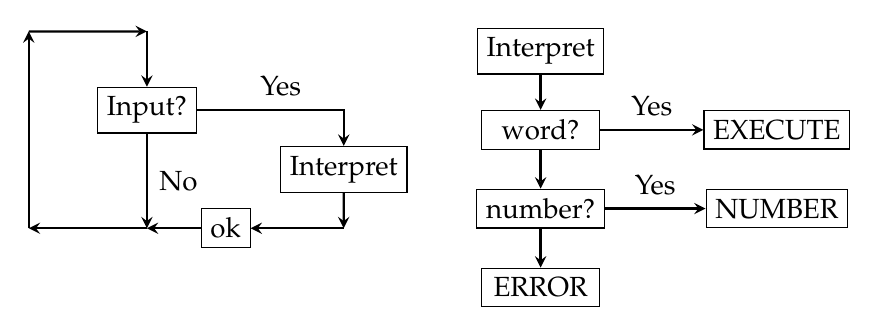
\begin{tikzpicture}[node distance=2cm]
            %Create nodes for left loop
            \node (input_1)     [wordinr1] {Input?}    ;
            \node (interpret_1) [wordinr1, right of = input_1, xshift=0.5cm, yshift=-0.75cm] {Interpret};
            \node (ok)          [wordinr1, below of = input_1, xshift=1.0cm, yshift=0.5cm] {ok};
            \coordinate[below of=input_1, yshift=0.5cm] (cont_1);
            \coordinate[left  of=cont_1,  xshift=0.5cm] (cont_2);
            \coordinate[above of=cont_2, yshift=0.5cm] (cont_3);
            \coordinate[above of=input_1, yshift=-1.0cm] (cont_4);
            \coordinate[below of=input_1, xshift=2.5cm, yshift=0.5cm] (cont_5);
            %Connect left loop
            \draw [arrow] (input_1.south) -- node[xshift=0.40cm] {No} (cont_1.north);
            \draw [arrow] (ok.west)       -- (cont_1.east);
            \draw [arrow] (cont_1.west)   -- (cont_2.east);
            \draw [arrow] (cont_2.north)  -- (cont_3.south);
            \draw [arrow] (cont_3.east)   -- (cont_4.west);
            \draw [arrow] (cont_4.south)  -- (input_1.north);
            %Connect right loop
            \draw [arrow] (input_1.east)  -| node[yshift=0.30cm, xshift=-0.80cm] {Yes} (interpret_1.north) ;
            \draw [arrow] (interpret_1.south) -- (cont_5.north);
            \draw [arrow] (cont_5.west) -- (ok.east) ;
            
            \node (interpret_2) [wordinr2, yshift=0.75cm, xshift=5.0cm]           {Interpret} ;
            \node (word)        [wordinr2, yshift=1.0cm,  below of = interpret_2] {word?}     ;
            \node (number_1)    [wordinr2, yshift=1.0cm,  below of = word, ]      {number?}   ;
            \node (error)       [wordinr2, yshift=1.0cm,  below of = number_1]    {ERROR}     ;
            \node (execute)     [wordinr2, xshift=1.0cm,  right of = word]        {EXECUTE}   ;
            \node (number_2)    [wordinr2, xshift=1.0cm,  right of = number_1]    {NUMBER}    ;
            \draw [arrow] (interpret_2) -- (word);
            \draw [arrow] (word)        -- (number_1);
            \draw [arrow] (number_1)    -- (error);
            \draw [arrow] (word)        -- node[yshift=0.30cm] {Yes} (execute);
            \draw [arrow] (number_1)    -- node[yshift=0.30cm] {Yes} (number_2);
        \end{tikzpicture}
    }
  \caption{\textit{Overview of FORTH outer interpreter}}
  \label{fig:02_01}
\end{figure}

In general, because FORTH is interpretive as well as compiled, the best way to study something new is in front of a computer running FORTH. Therefore we explain with illustrations, expecting the reader to try them out.

In what follows, anything the user types in will be set in \lstinline$Helvetica$, such as \regc{DECIMAL} below.

Machine responses appear in ordinary type.

We now give a trivial illustration:

\begin{lstlisting}
    DECIMAL <cr> ok
\end{lstlisting}

\Note \textbf{\underline{s:}}
\begin{itemize}
  \item \bc{<cr>} means "the user pushes the ENTER or $\Leftarrow$ button".
  \item \bc{ok} is what FORTH says in response to an input line, if nothing has gone wrong.
  \item \regc{DECIMAL} is an instruction to use base 10 arithmetic. FORTH will use any base on tell it, within reason, but usually only \regc{DECIMAL} and \regc{HEX} (hexadecimal) are predefined.
\end{itemize}

When the outer interpreter (see Fig. \ref{fig:02_01}, p. \pageref{fig:02_01}) encounters text with no dictionary entry, it tries to interpret it as a \bc{NUMBER}.

It places the number in a special memory location called "the top of the stack" (TOS)\sepfootnote{02_05}
\begin{lstlisting}
    2 17 +. <cr> 19 ok
\end{lstlisting}

\Note \textbf{\underline{s:}}
\begin{itemize}
  \item FORTH interprets 2 and 17 as numbers, and pushes them onto the stack. "\bc{+}" is a word and so is "\bc{.}" so they are \bc{EXECUTE}d.
  \item \bc{+} adds 2 to 17 and leaves 19 on the stack.
  \item The word \bc{.} (called "emit") removes 19 from the stack and displays it on the screen.
\end{itemize}

We might also have said\sepfootnote{02_06}

\begin{lstlisting}
    HEX 0A 14 * . <cr> C8 ok
\end{lstlisting}

(Do you understand this? Hint: \bc{HEX} stands for "switch to hexadecimal arithmetic")

If the incoming text can neither be located in the dictionary nor interpreted as a number, FORTH issues an error message.


\section{Extending the dictionary}

\TallC{The} compiler is one of FORTH's most endearing features. It is elegant, simple, and mostly written in FORTH. Although the technical details of the FORTH compiler are generally more interesting to systems developers than to scientists, its components can often be used to solve programming problems. When this is the case, we necessarily discuss details of the compiler. In this section we discuss how the compiler extends the dictionary. In \S2\S\S8 below we examine the parts of the compiler in greater detail.

FORTH has special words that allow the creation of new dictionary entries, \ie, new words. The most important are "\bc{:}" ("start a new definition") and "\bc{;}" ("end the new definition").

Consider the phrase

\begin{lstlisting}
    : NEW-WORD WORD1 17 WORDZ . . . WORDn ; ok
\end{lstlisting}

The initial "\bc{:}" is \bc{EXECUTE}d because it is already in the dictionary. Upon execution, "\bc{:}" does the following:

\begin{itemize}
    \item Creates a new dictionary entry, \bc{NEW-WORD}, and switches from \textbf{interpret}- to \textbf{compile} mode.
    \item In compile mode, the interpreter looks up words and --rather than executin them-- installs ointers to their code. If the text is a number (\bc{17} above), FORTH builds the literal number into the dictionary space allotted for \bc{NEW-WORD}.
    \item The action of \bc{NEW-WORD} will be to \bc{EXECUTE} sequentially the previously-defined words \bc{WORD1}, \bc{WORD2}, ...\bc{WORDn}, placing any built-in numbers on the stack as they occur.
    \item The FORTH compiler \bc{EXECUTE}s the last word "\bc{;}" of the definition, by installing code (to return control to the next outer level of the interpreter\sepfootnote{02_07}) then switching back from compile to interpret mode. Most other languages treat tokens like "\bc{;}" as flags (in the input stream) that \textit{trigger} actions, rather than actions in their own right FORTH lets components execute themselves.
\end{itemize}

In FORTH \textit{all} subroutines are words that are invoked when they are named. No explicit CALL or GOSUB statement is required.

The above definition of \textbf{NEW-WORD} is extremely structured compared with FORTRAN or BASIC. Its definition is just a series of subroutine calls.

\TallC{We} now illustrate how to define and use a new word using the previously defined words "\bc{:}"and "\bc{;}". Enter the phrase (this new word \bc{*+} expects 3 numbers, \textit{a}, \textit{b}, and \textit{c} on the stack)

\begin{lstlisting}
    : *+   * + ; ok
\end{lstlisting}

\Note \underline{\textbf{s:}}
\begin{itemize}
    \item \bc{*} multiplies \verb|b| with \verb|c|, leaving \verb|b*c|.
    \item \bc{+} then adds \verb|b*c| to \verb|a|, leaving \verb|a + b*c| behind.
\end{itemize}

Now we actually try out \bc{*+} :

\begin{lstlisting}
    DECIMAL 5 6 7 *+ . 47 ok
\end{lstlisting}

\Note \underline{\textbf{s:}}
\begin{itemize}
    \item The period \bc{.} is not a typo, it EMITs the result.
    \item FORTH's response to \bc{a b c *+ .} is \bc{a + b*c ok}.
\end{itemize}

What if we were to enter \bc{*+} with nothing on the stack? Let's try it and see (\bc{.S} is a word that displays the stack without changing its contents):

\begin{lstlisting}
    .S empty stack ok

    *+ empty stack ok
\end{lstlisting}

\dotrule{1\textwidth}

\underline{\textbf{Exercise:}}

Suppose you entered the input line

\begin{lstlisting}
    HEX 5 6 7 *+ . <cr> xxx ok
\end{lstlisting}

What would you expect the response \textbf{xxx} to be?

\textit{Answer:} \bc{2F}

\dotrule{1\textwidth}

\section{Stacks and reverse Polish notation (RPN)}
\TallC{We} now discuss the stack and the "reverse Polish" or "postfix" arithmetic based on it. (Anyone who has used one of the Hewlett-Packard calculators should already be familiar with the basic concepts.)

A Polish mathematician (J .Lukasewcleia) showed that numerical calculations require an irreducible minimum of elementary operations (fetching and storing numbers as well as addition, subtraction, multiplication and division). The minimum is obtained when the calculation is organized by "stack" arithmetic.

Thus virtually all central processors (CPU's) intended for arithmetic operations are designed around stacks. FORTH makes efficient use of CPU's by reflecting this underlying stack architecture in its syntax, rather than translating algebraic-looking program statements ("infix" notation) into RPN-based machine operations as FORTRAN, BASIC, C and Pascal do.

But what \textit{is} a stack? As the name implies, a stack is the machine analog of a pile of cards with numbers written on them. Numbers are always added to, and removed from, the top of the pile. (That is, a stack resembles a job where layoffs follow seniority: last in, first out.) Thus, the FORTH input line

\begin{lstlisting}
    DECIMAL 2 5 73 -16 ok
\end{lstlisting}

followed by the line

\begin{lstlisting}
    + - * . yyy ok
\end{lstlisting}
leaves the stack in the successive states shown in Table \ref{tab:02_01} below

\begin{table}
    \begin{center}
        \begin{tabular}{|c c c c c c c|}
            \hline
       Cell\# & Initial    & Ops$\rightarrow$ & +       & -          & *       & . \\ 
            \hline
            0 & \lgray -16 & Result        & \Aggray 57 & \dgray -52 & \gray 104 & ... \\ 
            1 & \lgray 73  & $\rightarrow$ & \Aggray 5  & \dgray 2   & ...       & ... \\
            2 & \lgray 5   &               & \Aggray 2  & ...        & ...       & ... \\
            3 & \lgray 2   &               & ...        & ...        & ...       & ... \\
            \hline
        \end{tabular}
    \end{center}
    \caption{\textit{Picture of the stack during operations}}
    \label{tab:02_01}
\end{table}

We usually employ zero-based relative numbering in FORTH data structures --stacks, arrays, tables, \etc-- so TOS ("top of stack") is given relative \#0, NOS ("next on stack") \#1, \etc

The operation "\bc{.}" ("emit") displays -104 to the screen, leaving the stack empty. That is, \bc{yyy} above is \bc{-104}.

\subsection{Manipulating the parameter stack}

\TallC{FORTH} system incorporate (at least) two stacks: the \textbf{parameter stack} which we now discuss, and the \textbf{return stack} which we defer to \S2.3.2.

In order to use a stack-based system, we must be able to put numbers on the stack, remove them, and rearrange their order. FORTH includes standard words for this purpose.

Putting numbers on the stack is easy: one simply types the number (or it appears in the definition of a FORTH word).

To remove a number we have the word \bc{DROP} that drops the number from TOS and moves up all the other numbers.

To exchange the top 2 numbers we have .

\bc{DUP} duplicates the TOS into NOS, pushing down all the other numbers.

\bc{ROT} rotates the top 3 numbers.

\begin{table}
    \begin{center}
        \begin{tabular}{|c c c c c c c|}
            \hline
       \textbf{Cell\#} & Initial    & \textbf{Ops$\rightarrow$} & \textbf{DROP}   & \textbf{SWAP}        & \textbf{ROT}       & \textbf{DUP}\\  
            \hline
            0 & \lgray -16 & \textbf{Result}        & \Aggray 73 & \dgray 73  & \gray 5   & \digray -16 \\ 
            1 & \lgray 73  & \textbf{$\rightarrow$} & \Aggray 5  & \dgray -16 & \gray -16 & \digray -16 \\
            2 & \lgray 5   &               & \Aggray 2  & \dgray 5   & \gray 73  & \digray 73  \\
            3 & \lgray 2   &               & ...        & \dgray 2   & \gray 2   & \digray 5   \\
            4 & \lgray ... &               & ...        & ...        & ...       & \digray 2   \\
            \hline
        \end{tabular}
    \end{center}
    \caption{\textit{Stack manipulation operators}}
    \label{tab:02_02}
\end{table}

These actions are shown on page \pageref{tab:02_02} above in Table \ref{tab:02_02} (we show what each word does to the initial stack).

In addition the words \bc{OVER}, \bc{UNDER}, \bc{PICK} and \bc{ROLL} act as shown in Table \ref{tab:02_03} below (note \bc{PICK} and \bc{ROLL} must be preceded by an integer that says where on the stack an element gets  \bc{PICK}ed or \bc{ROLL}ed).

\begin{table}
    \begin{center}
        \begin{tabular}{|c c c c c c c|}
            \hline
       \textbf{Cell\#} & Initial    & \textbf{Ops$\rightarrow$} & \textbf{OVER}   & \textbf{UNDER}        & \textbf{4 PICK}  & \textbf{4 ROLL}\\ [0.5ex] 
            \hline
            0 & \lgray -16 & \textbf{Result}        & \Aggray 73  & \dgray -16 & \gray 2   & \digray 2   \\ 
            1 & \lgray 73  & \textbf{$\rightarrow$} & \Aggray -16 & \dgray 73  & \gray -16 & \digray -16 \\
            2 & \lgray 5   &               & \Aggray 73  & \dgray -16 & \gray 73  & \digray 73  \\
            3 & \lgray 2   &               & \Aggray 5   & \dgray 5   & \gray 5   & \digray 5   \\
            4 & \lgray ... &               & \Aggray 2   & \dgray 2   & \gray 2   & ...         \\
            \hline
        \end{tabular}
    \end{center}
    \caption{\textit{More stack manipulation operators}}
    \label{tab:02_03}
\end{table}

Clearly, \bc{1 PICK} is the same as \bc{DUP}, \bc{2 PICK} is a synonym for \bc{OVER}, \bc{2 ROLL} means \bc{SWAP}, and \bc{3 ROLL} means \bc{ROT}.

As Brodie has noted (\TF), it is rarely advisable to have aword use a stack so deep that \bc{PICK} or \bc{ROLL} is needed. It is generally better to keep word definitions short, using only a small number of arguments on the stack and consuming them to the extent possible. On the other hand, \bc{ROT} and its opposite, \bc{-ROT}\sepfootnote{02_08}, are often useful.

\subsection{The return stack and Its uses}
\TallC{We} have remarked above in \S2\S\S2 that compilation establishes links from the calling word to the previously- defined word being invoked. Part of the linkage mechanism --during actual execution-- is the \textbf{return stack} (rstack): the address of the next word to be invoked after the currently executing word is placed on the rstack, so that when the current word is done, the system jumps to the next word. Although it might seem logical to call the address on the rstack the \textbf{next} address, it is actually called the \textbf{return} address for historical reasons.

In addition to serving as a reservoir of return addresses (since words can be nested, the return addresses need a stack to be put on) the rstack is where the limits of a \bc{DO ... LOOP} construct are placed\sepfootnote{02_09}.

The user can also store/retrieve to/from the rstack This is an example of using a component for a purpose other than the one it was designed for. Such use is not encouraged by every FORTH text, needless to say, since it introduces the spice of danger. To store to the rstack we say \bc{>R}, and to retrieve we say \bc{R>}. \bc{DUP>R} is a speedup of the phrase \bc{DUP >R}. The words \bc{D>R DR>} , for maving double-length integers, also exist on many systems. The word \bc{R@} copies the top of the rstack to the TOS.

\leftbar[1\linewidth]
\textbf{The danger is this:} anything put on the rstack during a word’s execution must be removed before the word terminates. If the \bc{>R} and the \bc{R>} do not balance, then a \textbf{wrong next address} will be jumped to and \bc{EXECUTE}d. Since this could be the address of data, and since it is being interpreted as machine instructions, the results will be \textbf{always unpredictable}, but seldom amusing.
\endleftbar

\TallC{Why} would we want to use the rstack for storage when we have a perfectly good parameter stack to play with? Sometimes it becomes simply impossible to read code that performs complex gymnastics on the parameter stack, even though FORTH permits such gymnastics.

Consider a problem --say, drawing a line on a bit- mapped graphics output device from (x,y) to (x',y')-- that requires 4 arguments. We have to turn on the appropriate pixels in the memory area representing the display, in the ranges from the origin to the end coordinates of the line. Suppose we want to work with x and y first, but they are 3rd and 4th on the stack. So we have to \bc{ROLL} or \bc{PICK} to get them to TOS where they can be worked with conveniently. We probably need them again, so we use

\begin{lstlisting}
    4PICK 4PICK ( -- x y x' y' x y)
\end{lstlisting}

Now 6 arguments are on the stack! See what I mean? A better way stores temporarily the arguments x’ and y', leaving only 2 on the stack. If we need to duplicate them, we can do it with an already existing word, \bc{DDUP}.

Complex stack manipulations can be avoided by defining \bc{VARIABLE}s --named locations-- to store numbers. Since FORTH, variables are typically \textit{global} --any word can access them-- their use can lead to unfortunate and unexpected interactions among parts of a large program. Variables should be used sparingly.

While FORTH permits us to make variables local to the sub- if routines that use them\sepfootnote{02_10}, for many purposes the rstack can advantageously replace local variables:

\begin{itemize}
    \item The rstack already exists, so it need not be defined anew.
    \item When the numbers placed on it are removed, the rstack shrinks, thereby reclaiming some memory.
\end{itemize}

Suppose, in the previous example, we had put x’ and y’ on the rstack via the phrase

\begin{lstlisting}
    >R >R DDUP .
\end{lstlisting}

Then we could duplicate and access x and y with no trouble.

\leftbar[1\linewidth]
\underline{\textbf{A note of caution}}: since the rstack is a critical component of the execution mechanism, we mess with it at our peril. If we want to use it, we must clean up when we are done, so it is in the same state as when we found it. A word that places a number on the rstack must get it off again --using \bc{R>} or \bc{RDROP}-- before exiting that word\footnotemark. Similarly, since \bc{DO ... LOOP} uses the rstack also, for each \bc{>R} in such a loop (after \bc{DO}) there must be a corresponding \bc{R>} or \bc{RDROP} (before \bc{LOOP} is reached). Otherwise the results will be unpredictable and probably will crash the system.
\endleftbar

\footnotetext{{\textbf{RDROP} is a handy way to exit from a word before reaching the final ";". See \TF.}}

\section{Fetching and storing}

\TallC{Ordinary} (16-bit) numbers are f\textit{etc}hed from memory to the stack by "\bc{@}" ("fetch"), and stored by "\bc{!}" ("store"). The word @ expects an address on the stack and replaces that address by its contents using, \textit{e.g.}, the phrase \bc{X @}. The word "\regc{!}" expects a number (NOS) and an address (TOS) to store it in, and places the number in the memory location referred to by the address, consuming both arguments in the process, as in the phrase \bc{32 X !}

Double length (32-bit) numbers can similarly be f\textit{etc}hed and stored, by \bc{D@} and \bc{DI} . (FORTH systems designed for the newer 32-bit machines sometimes use a 32-bit-wide stack and may not distinguish between single- and double-length integers.)

Positive numbers smaller than 255 can be placed in single bytes of memory using \bc{C@} and \bc{C!}. This is convenient for operations with strings of ASCII text, for example screen, file and keyboard I/O.

In Chapters 3, 4, 5 and 7 we shall extend the lexicon of \bc{@} and \bc{!} words to include floating point and complex numbers.

\section{Arithmetic operations}

\TallC{The} 1979 or 1983 standards, not to mention the forthcoming ANSII standard, require that a conforming FORTH system contain a certain minimum set of predefined words. These consist of arithmetic operators \bc{+ - * / MOD /MOD */} for (usually) 16-bit \textit{signed-integer} (-32767 to +32767) arithmetic, and equivalents for \textit{unsigned} (0 to 65535), double-length and mixed-mode (16- mixed with 32-bit) arithmetic. The list will be found in the glossary accompanying your system, as well as in \SF and \FTR.

\section{Comparing and testlng}

\TallC{In} addition to arithmetic, FORTH lets us compare numbers on the stack, using relational operators \bc{> < =}.These operators work as follows: the phrase

\begin{lstlisting}
    2 3 > <cr> ok
\end{lstlisting}

will leave 0 ("false") on the stack, because 2 (N0S) is not greater
than 3 (TOS). Conversely, the phrase

\begin{lstlisting}
    2 3 < <cr> ok
\end{lstlisting}

will leave -1 ("true") because 2 is less than 3. Relational operators typically consume their arguments and leave a "flag" to show what happened\sepfootnote{02_12}. Those listed so far work with signed 16-bit integers. The operator \bc{U<} tests \textit{unsigned} 16-bit integers (0-65535).

FORTH offers unary relational operators \bc{0= 0>} and \bc{0<} that determine whether the TOS contains a (signed) 16-bit integer that is 0, positive or negative. Most FORTHs offer equivalent relational operators for use with double-length integers.

The relational words are used for branching and control. The usual form is

\begin{lstlisting}
    : MAYBE 0> IF WORDl WORD2 ...
      WORDn THEN ;
\end{lstlisting}

The word \bc{MAYBE} expects a number on the stack, and executes the words between \bc{IF} and \bc{THEN} if the number on the stack is positive, but not otherwise. If the number initially on the stack were negative or zero, \bc{MAYBE} would do nothing.

An alternate form including \bc{ELSE} allows two mutually exclusive actions:

\begin{lstlisting}
    : CHOOSE 0> IF WORD1 . . . WORDn
            ELSE WORDt' . . . WORDn'
            THEN ; (n -- )
\end{lstlisting}

If the number on the stack is positive, \bc{CHOOSE} executes \bc{WORD1 WORD2... WORD}, whereas if the number is negative or 0, \bc{CHOOSE} executes \bc{WORD1'} ... \bc{WORDn'}.

In either example, \bc{THEN} marks the end of the branch, rather than having its usual logical meaning\sepfootnote{02_13}.

\section{Looping and structured programming}

\TallC{FORTH} contains words for setting up loops that can be definite or indefinite:

\begin{lstlisting}
    BEGIN xxx flag UNTIL
\end{lstlisting}

The words represented by \bc{xxx} are executed, leaving the TOS (flag) set to 0 (F) -at which point \bc{UNTIL} leaves the loop - or -1 (T) -at which point \bc{UNTIL} makes the loop repeat from \bc{BEGIN}.

A variant is
\begin{lstlisting}
    BEGIN xxx flag WHILE yyy REPEAT
\end{lstlisting}

Here \bc{xxx} is executed, \bc{WHILE} tests the flag and if it is 0 (F) leaves the loop; whereas if flag is -1 (T) \bc{WHILE} executes \bc{yyy} and \bc{REPEAT} then branches back to \bc{BEGIN}. These forms can be used to set up loops that repeat until some external event (pressing a key at the keyboard, \textit{e.g.}) sets the flag to exit the loop. They can also used to make endless loops (like the outer interpreter of FORTH) by forcing flag to be 0 in a definition like

\begin{lstlisting}
    : ENDLESS BEGIN xxx 0 UNTIL ;
\end{lstlisting}

\TallC{FORTH} also implements indexed loops using the words \bc{DO LOOP +LOOP /LOOP}. These appear within definitions, \textit{e.g.}

\begin{lstlisting}
    : LOOP-EXAMPLE 100 0 DO xxx LOOP ;
\end{lstlisting}

The words \bc{xxx} will be executed 100 times as the lower limit, 0, increases in unit steps to 99. To step by -2's, we use the phrase

\begin{lstlisting}
    -2 + LOOP
\end{lstlisting}

to replace \bc{LOOP}, as in

\begin{lstlisting}
    : DOWN-BY-2's O 100 DO xxx -2 +LOOP ;
\end{lstlisting}

The word \bc{/LOOP} 1s a variant of \bc{+LOOP} for working with unsigned limits\sepfootnote{02_14} and increments (to permit the loop index to go up to 65535 in 16-bit systems).

\section{The pearl of FORTH}

An unusual construct, \bc{CREATE...DOES>}, has been called "the pearl of FORTH" \sepfootnote{02_15}. This is more than poetic license.

\bc{CREATE} is a component of the compiler that makes a new dictionary entry with a given name (the next name in the input stream) and has no other function.

\bc{DOES>} assigns a specific run-time action to a newly \bc{CREATE}d word (we shall see this in \S2\S\S8-3 below).

\subsection{Dummy words}
Sometimes we use \bc{CREATE} to make a dummy entry that we can later assign to some action:
\begin{lstlisting}
    CREATE DUMMY
    CA' * DEFINES DUMMY
\end{lstlisting}

The second line translates as "The code address of \bc{*} defines \bc{DUMMY}". Entry of the above phrase would let \bc{DUMMY} perform the job of \bc{*} just by saying \bc{DUMMY}. That is, FORTH lets us first define a dummy word, and then give it any other word’s meaning \sepfootnote{02_16}.

Here is one use of this power: Suppose we have to define two words that are alike except for some piece in the middle:
\begin{lstlisting}
    : *WORD  WORD1 WORD2 *  WORD3 WORD4 ;
    : */WORD WORD1 WORD2 */ WORD3 WORD4 ;
\end{lstlisting}

we could get away with 1 word, together with \bc{DUMMY} fromabove,

\begin{lstlisting}
    : *_or_*/WORD
        WORD1 WORD2
        DUMMY
        WORD3 WORD4 ;
\end{lstlisting}
by saying
\begin{lstlisting}
    CA' * DefinES DUMMY *_or_*/WORD
\end{lstlisting}
or
\begin{lstlisting}
    CA' */ DefinES DUMMY *_or_*/WORD
\end{lstlisting}

This technique, a rudimentary example of vectoring, saves memory and saves programming time by letting us vary something in the middle of a definition \textit{after the definition has been entered in the dictionary}. However, this technique must be used with caution as it is akin to \textbf{self-modifying} code\sepfootnote{02_17}.

A similar procedure lets a subroutine call itself recursively, an enormous help in coding certain algorithms.

\subsection{Defining "defining" words}

\TallC{The} title of this section is neither a typo nor a stutter: \bc{CREATE} finds its most important use in extending the powerful class of FORTH words called "defining" words. The colon compiler "\bc{:}" is such a word, as are \bc{VARIABLE} and \bc{CONSTANT}. The definition of \bc{VARIABLE} is simple

\begin{lstlisting}
    : VARIABLE CREATE 2 ALLOT ;
\end{lstlisting}

Here is how we use it:
\begin{lstlisting}
    VARIABLE X <cr> ok
\end{lstlisting}

The inner workings of VARIABLE are these:
\begin{itemize}
    \item \bc{CREATE} makes a dictionary entry with the next name in the input stream -- in this case, \bc{X}.
    \item Then the number 2 is placed on the stack, and the word \bc{ALLOT} increments the pointer that represents the current location in the dictionary by 2 bytes.
    \item This leaves a 2-byte vacancy to store the value of the variable (that is, the next dictionary header begins 2 bytes above the end of the one just defined).
\end{itemize}

When the outer interpreter loop encounters a new \bc{VARIABLE}'s name in the input stream, that name’s address is placed on the stack. But this is also the location where the 2 bytes of storage begins. Hence when we type in \bc{X}, the TOS will contain the storage address named \bc{X}.

As noted in \S2.4 above, the phrase \bc{X @} (pronounced "X f\textit{etc}h") places the contents of address \bc{X} on the stack, dropping the address in the process. Conversely, to store a value in the named location \bc{X}, we use \bc{!} ("store"): thus
\begin{lstlisting}
    4 X ! <cr> ok
    X @ . <cr> 4 ok
\end{lstlisting}

Double-length variables are defined \textit{via} \bc{DVARIABLE}, whose definition is

\begin{lstlisting}
    : DVARIABLE CREATE 4 ALLOT ;
\end{lstlisting}

\TallC{FORTH} has a method for defining words initialized to contain specific values: for example, we might want to define the number 17 to be a word. \bc{CREATE} and "\bc{,}" ("comma") let us do this as follows:

\begin{lstlisting}
    17 CREATE SEVENTEEN , <cr> ok
\end{lstlisting}

Now test it \textit{via}

\begin{lstlisting}
    SEVENTEEN @ . <cr> 17 ok
\end{lstlisting}

\leftbar[1\linewidth]
\Note: The word "," ("comma") puts TOS into the next 2 bytes of the dictionary and increments the dictionary pointer by 2.

A word \bc{C}, ("see-comma") puts a byte-value into the next byte of the dictionary and increments the pointer by 1 byte.
\endleftbar

\subsection{Run-time vs. compile-time actions}

\TallC{In} the preceding example, we were able to initialize the variable \bc{SEVENTEEN} to 17 when we \bc{CREATE}d it, but we still have to fetch it to the stack \textit{via} \bc{SEVENTEEN @} whenever we want it. This is not quite what we had in mind: we would like to find 17 in T0S when we say \bc{SEVENTEEN}. The word \bc{DOES>} gives us precisely the tool to do this.

As noted above, the function of \bc{DOES>} is to specify a run-time action for the "child" words of a defining word. Consider the defining word \bc{CONSTANT}, defined in high-level\sepfootnote{02_18} FORTH by

\begin{lstlisting}
    : CONSTANT CREATE , DOES> @ ;
\end{lstlisting}
and used as
\begin{lstlisting}
    53 CONSTANT PRIME ok
\end{lstlisting}

Now test it:
\begin{lstlisting}
    (*\bfseries PRIME*) . <cr> 53 ok
\end{lstlisting}

What happened?
\begin{itemize}
    \item \bc{CREATE} (hidden in \bc{CONSTANT}) made an entry (named \bc{PRIME} , the first word in the input stream following \bc{CONSTANT}). Then "\bc{,}" placed the TOS (the number 53) in the next two bytes of the dictionary.
    \item \bc{DOES>} (inside \bc{CONSTANT}) then appended the actions of all words between it and "\bc{;}" (the end of the definition of \bc{CONSTANT}) to the child word(s) defined by \bc{CONSTANT}.
    \item In this case, the only word between \bc{DOES>} and \bc{;} was \bc{@} , so all FORTH constants defined by \bc{CONSTANT} perform the action of placing their address on the stack (anything made by \bc{CREATE} does this) and fetching the contents of this address.
\end{itemize}

\subsubsection{Klingons}

\TallC{Let} us make a more complex example. Suppose we had previously defined a word \bc{BOX ( n x y -- )} that draws a small square box of n pixels to a side centered at (x, y) on the graphics display. We could use this to indicate the instantaneous location of a moving object -- say a Klingon space-ship in a space-war game.

So we define a defining word that creates (not very realistic looking) space ships as squares n pixels on a side:

\begin{lstlisting}
    : SPACE-SHIP CREATE , DOES>
        @-ROT (--nxy)      BOX ;
    : SIZE ; \ do-nothing word
\end{lstlisting}

Now, the usage would be (\bc{SIZE} is included merely as a reminder of what 5 means -- it has no function other than to make the definition look like an English phrase)

\begin{lstlisting}
    SIZE 5 SPACE-SHIP KLINGON <cr> ok
    71 35 KLINGON <cr> ok
\end{lstlisting}

Of course, \bc{SPACE-SHIP} is a poorly constructed defining word because it does not do what it is intended to do. Its child-word \bc{KLINGON} simply draws itself at (x, y).

What we really want is for \bc{KLINGON} to \textit{undraw} itself from its old location, compute its new position according to a set of rules, and then redraw itself at its new position This sequence of operations would require a definition more like

\begin{lstlisting}
    :OLD.POS@ (adr--adr n x y) DUP @ OVER
      2+ D@ :
    : SPACE-SHIP CREATE , 4 ALLOT DOES>
       OLD.POS@ UNBOX NEW.POS!
       OLD.POS@ BOX DROP ;
\end{lstlisting}

where the needed specialized operation \bc{UNBOX} would be defined previously along with \bc{BOX}.

\subsubsection{Dimensioned data (with intrinsic unlts)}
Here is another example of the power of defining words and of the distinction between compile-time and run-time behaviors.

Physical problems generally work with quantities that have dimensions, usually expressed as mass (M), length (L), and time (T) or products of powers of these. Sometimes there is more than one system of units in common use to describe the same phenomena.

For example, traffic police reporting accidents in the United States or the United Kingdom might use inches, feet, and yards; whereas Continental police would use the metric system. Rather than write different versions of an accident analysis program it is simpler to write one program and make unit conversions part of the grammar. This is easy in FORTH; impossible in FORTRAN, BASIC, Pascal, or C; and possible, but exceedingly cumbersomein Ada\sepfootnote{02_19}.

We simply keep all internal lengths in millimeters, say, and con-
vert as follows\sepfootnote{02_20}:

\begin{lstlisting}
    : INCHES  254 10 */ ;
    : FEET  [ 254 12 * ] LITERAL 10 */ ;
    : YARDS [ 254 36 * ] LITERAL 10 */ ;
    : CENTIMETERS 10 * ;
    : METERS 1000 * ;
\end{lstlisting}

The usage would be
\begin{lstlisting}
    10 FEET . <cr> 3048 ok
\end{lstlisting}

These are more definitions than necessary, of course, and the technique generates unnecessary code. A more compact approach uses a \textit{defining word}, \bc{UNITS}:

\begin{lstlisting}
    : D, SWAP , , ; \ I double-length # in next cells
    : UNITS CREATE D, DOES> D@ */ ;
\end{lstlisting}

Then we could make the table
\begin{lstlisting}
    254  10         UNITS INCHES
    254  12 * 10    UNITS FEET
    254  36 * 10    UNITS YARDS
     10   1         UNITS CENTIMETERS
    1000  1         UNITS METERS
    \ Usage:
    \ 10 FEET . <cr> 3048 ok
    \ 3  METERS . <cr> 3000 ok
    \ ......
    \ (*\etc*).
\end{lstlisting}

This is an improvement, but FORTH lets us do even better: here is a simple extension that allows conversion back to the input units, for use in output:

\begin{lstlisting}
    VARIABLE <AS>                \ new variable
    0 <AS> !                     \ initialize to "F"
    : AS -1 <AS> ! ;             \ set <AS> = "T"
    : UNITS CREATE D, DOES>
       D@                        \ get 2 #s
       <AS> @                    \ get current val.
          IF SWAP THEN           \ flip if "true"
      */   0 <AS> ! ;            \ convert, reset <AS>

    BEHEAD' <AS>          \ make it local for security(*\sepfootnote{02_21}*)
    \ unit definitions remain the same
    \ Usage:
    \ 10 FEET      . <cr> 3048 ok
    \ 3048 AS FEET . <cr> 10 ok
\end{lstlisting}

\subsection{Advanced methods of controlllng the compiler}

\TallC{FORTH} includes a technique for switching from compile mode to interpret mode while compiling or interpreting. This is done using the words \bc{]} and \bc{[} . (Contrary to intuition, \bc{]} turns the compiler on, \bc{[} turns it off.)

One use of \bc{]} and \bc{[} is to create an "action table" that allows us to choose which of several actions we would like to perform\sepfootnote{02_22}.

For example, suppose we have a series of push-buttons numbered 1-6, and a word \bc{WHAT} to read them.

That is, \bc{WHAT} waits for input from a keypad; when button \#3 is pushed, \eg, \bc{WHAT} leaves 3 on the stack.

We would like to use the word \bc{BUTTON} in the following way:

\begin{lstlisting}
    WHAT BUTTON
\end{lstlisting}

\bc{BUTTON} can be defined to choose its action from a table of
actions called \bc{BUTTONS} . We define the words as follows:

\begin{lstlisting}
    CREATE BUTTONS ] RING-BELL OPEN-DOOR
      ENTER LAUGH CRY SELF-DESTRUCT [
    : BUTTON 1- 2* BUTTONS + @ EXECUTE ;
\end{lstlisting}

If, as before, I push \#3, then the action \bc{ENTER} will be executed. Presumably button \#7 is a good one to avoid\sepfootnote{02_23}.

How does this work?
\begin{itemize}
    \item \bc{CREATE BUTTONS} makes a dictionary entry \bc{BUTTONS}.
    \item \bc{]} turns on the compiler: the previously-defined word-names \bc{RING-BELL}, \textit{etc.} are looked up in the dictionary and compiled into the table (as though we had begun with \bc{:}), rather than being executed.
    \item \bc{[} returns to interactive mode (as if it were ;), so that the next colon definition (\bc{BUTTON}) can be processed.
    \item The table \bc{BUTTONS} now contains the code-field addresses (CFA’s) of the desired actions of \bc{BUTTON}.
    \item \bc{BUTTON} first uses 1- to subtract 1 from the button number left on the stack by \bc{WHAT} (so we can use 0-based numbering into the table -- if the first button were \# 0, this would be unneeded).
    \item \bc{2*} then multiplies by 2 to get the offset (from the beginning of \bc{BUTTONS}) of the CFA representing the desired action.
    \item \bc{BUTTONS +} then adds the base address of \bc{BUTTONS} to get the absolute address where the desired CPA is stored.
    \item \bc{@} fetches the CFA for \bc{EXECUTE} to execute.
    \item \bc{EXECUTE} executes the word corresponding to the button pushed. Simple!
\end{itemize}

You may well ask "Why bother with all this indirection, pointers, pointers to pointers, tables of pointers to tables of pointers, and the like?" Why not just have nested \bc{IF...ELSE...THEN} constructs, as in Pascal?

There are three excellent reasons for using pointers:
\begin{itemize}
    \item Nested \bc{IF...THEN}'s uickly become cumbersome and difficult to decipher (\TF). They are also \underline{\textbf{slow}} (see Ch. 11).
    \item Changing pointers is generally much faster than changing other kinds of data -- for example reading in code overlays to accomplish a similar task.
    \item The unlimited depth of indirection possible in FORTH permits arbitrary levels of abstraction. This makes the computer behave more "intelligently" than might be possible with more restrictive languages.
\end{itemize}

A similar facility with pointers gives the C language its abstractive power, and is a major factor in its popularity.

\section{Strings}

\TallC{By} now it should be apparent that FORTH can do anything any other language can do. One feature we need in any sort of programming --scientific or otherwise-- is the ability to handle alphanumeric strings. We frequently want to print messages to the console, or to put captions on figures, even if we have no interest in major text processing.

While every FORTH system must include words to handle strings(see, e.g., \FTR Ch. 9) --the very functioning of the outer interpreter, compiler, \textit{etc.}, demands this-- there is little unanimity in defining extensions. BASIC has particularly good string-handling features, so HS/FORTH and others provide extensions designed to mimic BASIC’s string functions.

Typical FORTH strings are Iimite to 255 characters because they contain a count in their first byte\sepfootnote{02_24}.The word \bc{COUNT}
\begin{lstlisting}
    : COUNT DUP 1+ SWAP C@ ; (adf--nadr+1)
\end{lstlisting}

expects the address of a counted string, and places the count and
the address of the first character of the string on the stack. \bc{TYPE}, a required '79 or '83 word, prints the string to the console.

It is straightforward to employ words that are part of the system (such as \bc{KEY} and \bc{EXPECT}) to define a word like \bc{$"} that takes all characters typed at the keyboard up to a final \bc{"} (close-quote --not a word but a string-terminator), makes a counted string of them, and places the string in a buffer beginning at an address returned by \bc{PAD}\sepfootnote{02_25}.

The word \bc{$.} ("string-emit") could then be defined as
\begin{lstlisting}
    : $. COUNT TYPE ; (adr --)
\end{lstlisting}

and would be used with \bc{$"} like this:
\begin{lstlisting}
    $" The quick brown fox" < cr> ok
    $. The quick brown fox ok
\end{lstlisting}

Since this book in not an attempt to paraphrase \FTR it is strongly recommended that the details of using the system words to devise a string lexicon be studied there.

\leftbar[1\linewidth]
One might contemplate modifying the \FTR lexicon by using a full 16-bit cell for the count. This would permit strings of up to 64k bytes (using unsigned integers\footnotemark), wasting 1 byte of memory per short ( 255 bytes) string. Although few scientific applications need to manipulate such long strings, the program that generated the index to this book needed to read a page at a time, and thus to handle strings about 3-5 kbytes long.
\endleftbar
\footnotetext{\FTR, Ch. 3.}

\section{FORTH programming style}

\TallC{A} FORTH program typically looks like this
\begin{lstlisting}
    \ Example of FORTH program
    :WORD1 ... ;
    :WORD2 OTHER-WORDS ;
    :WORDS YET-OTHER-WORDS ;
       ...
    : LAST-WORD WORDn ...WORD3
       WORD2 WORD1 ;
    LAST-WORD <cr> \ run program
\end{lstlisting}

\leftbar[1\linewidth]
\Note: The word {\textbackslash } means "disregard the rest of this line". It is a convenient method for commenting code.
\endleftbar

In other words, a FORTH program consists of a series of word definitions, culminating in a definition that invokes the whole shebang. This aspect gives FORTH programming a somewhat different flavor from programming in more conventional languages.

Brodie notes in \TF that high-level programming languages are considered good if they require structured, top-down programming, and \textit{wonderful} if they impose \textit{information hiding}. Languages such as FORTRAN, BASIC and assembler that permit direct jumps and do not impose structure, top-down design and data-hiding are considered \textit{primitive} or bad. To what extent does FORTH follow the norms of good or \textit{wonderful} programming practice?

\subsection{Structure}

\TallC{The} philosophy of "structured programming" entered the general consciousness in the early 1970’s. The idea was to make the logic of program control flow immediately apparent, thereby aiding to produce correct and maintainable programs. The language Pascal was invented to impose by fiat the discipline of structure. To this end, direct jumps (GOTOs) were omitted from the language\sepfootnote{02_27}.

FORTH programs are automatically structured because word definitions are nothing but subroutine calls. The language contains no direct jump statements (that is, no GOTO's) so it is \textit{impossible} to write "spaghetti" code.

A second aspect of structure that FORTH imposes (or at least encourages) is \textit{short} definitions. There is little speed penalty incurred in breaking a long procedure into many small ones, unlike more conventional languages. Each of the short words has one entry and one exit point, and does one job. This is the beaux ideal of structured programming!

\subsection{"Top-down" design}

\TallC{Most} authors of "how to program" books recommend designing the entire program from the general to the particular. This is called "top-down" programming, and embodies these steps:

\begin{itemize}
    \item Make an outline, flow chart, data-flow diagram or whatever, taking a broad overview of the whole problem.
    \item Break the problem into small pieces (decompose it).
    \item Then code the individual components.
\end{itemize}

The natural programming mode in FORTH is "bottom-up" rather than "top-down" -- the most general word appears last, whereas the definitions necessarily progress from the primitive to the complex. It is possible -- and sometimes vital -- to invoke a word before it is defined ("forward referencing"\sepfootnote{02_28}). The dictionary and threaded compiler mechanisms make this nontrivial. The naturalness of bottom-up programming encourages a somewhat different approach from more familiar languages:

\begin{itemize}
    \item In FORTH, components are specified roughly, and then 3 they are coded they are immediately tested, debugged, redesigned and improved.
    \item The evolution of the components guides the evolution of the outer levels of the program.
\end{itemize}

We will observe this evolutionary style in later chapters as we design actual programs.

\subsection{Information hiding}

\TallC{Information} (or data) "hiding" is another doctrine of structured programming. It holds that no subroutine should have access to, or be able to alter (corrupt!) data that it does not absolutely require for its own functioning\sepfootnote{02_29}.

Data hiding is used both to prevent unforeseen interactions between pieces of a large program; and to ease designing and debugging a large program. The program is broken into small, manageable chunks ("black boxes") called \textbf{modules} or \textbf{objects} that communicate by sending messages to each other, but are otherwise mutually impenetrable. Information hiding and modularization are now considered so important that special languages --Ada, MODULA-Z, C++, and Object Pascal-- have been devised with it in mind.

To illustrate the problem information hiding is intended to solve, consider a FORTRAN program that calls a subroutine

\begin{lstlisting}
    PROGRAM MAIN
        some lines
    CALL SUB1(arg1, ar92, ... , argn, answer)
        some lines
    END

    SUB1(X1, ... , Xn, Y)
        some lines
        Y = something
    RETURN
    END
\end{lstlisting}

There are two ways to pass the arguments from MAIN to SUB1, and FORTRAN can use both methods.

\begin{itemize}
    \item Copy the arguments from where they are stored in MAIN into locations in the address space of SUBl (set aside for them during compilation). If the STATEMENTS change the values X1,...,Xn during execution of SUBl, the original values in the callin program will not be affected (because they are stored elsew ere and were copied during the CALL).
    \item Let SUBl have the addresses of the arguments where they are stored in MAIN. This method is dangerous because if the arguments are changed during execution of SUBl, they are changed in MAIN and are forever corrupted. If these changes were unintended, they can produce remarkable bugs.
\end{itemize}

Although copying arguments rather than addresses seems safer, sometimes this is impossible either because the increased memory overhead may be infeasible in problems with large amounts of data, or because the extra overhead of subroutine calls may unacceptably slow execution.

What has this to do with FORTH?

\begin{itemize}
    \item FORTH uses linked lists of addresses, compiled into a dictionary to which all words have equal right of access.
    \item Since everything in FORTH is a word --constants, variables, numerical operations, I/O procedures-- it might seem impossible to hide information in the sense described above.
    \item Fortunately, word-names can be erased from the dictionary after their CFAs have been compiled into words that call them. (This erasure is called "beheading".)
    \item Erasing the names of variables arantees they can be neither accessed nor corrupted by unauthorized words (except through a calamity so drea ful the program crashes).
\end{itemize}

\subsection{Documenting and commenting FORTH code}

\TallC{FORTH} is sometimes accused of being a "write-only" language. In other words, some complain that FORTH is cryptic. I feel this is basically a complaint against poor documentation and unhelpful word names, as Brodie and others have noted.

Unreadability is equally a flaw of poorly written FORTRAN, Pascal, C, \textit{et al}.

FORTH offers a programmer who takes the trouble a goodly array of tools for adequately documenting code.

\subsubsection{Parenthesized remarks}
The word ( --a left parenthesis followed by a space-- says "disregard all following text up until the next right parenthesis\sepfootnote{02_30} in the input stream. Thus we can intersperse explanatory remarks within colon definitions. This method was used to comment the Legendre polynomial example program in Ch. 1.

\subsubsection{Stack comments}
A particular form of parenthesized remark describes the effect of a word on the stack (or on the floating point fstack in Ch. 3). For example, the stack-effect comment (stack comment, for short)

\begin{lstlisting}
    ( adr - - n )
\end{lstlisting}

would be appropriate for the word \bc{@} ("fetch"): it says \bc{@} expects to find an address (adr) on the stack, and to leave its contents (n) upon completion.

The corresponding comment for \bc{!} would be
\begin{lstlisting}
    ( n adr --).
\end{lstlisting}

An fstack comment is prefaced by a double colon :: as
\begin{lstlisting}
    (::x -- f[x]).
\end{lstlisting}

Note that to replace parentheses within the comment we use brackets [ ] , since parentheses would be misinterpreted. Since the brackets appear to the right of the word \bc{(} , they cannot be (mis-)interpreted as the FORTH words \bc{]} or \bc{[}.

With some standard conventions for names\sepfootnote{02_31}, and standard abbreviations for different types of numbers, the stack comment may be all the documentation needed, especially for a short word.

\subsubsection{Drop line (\textbackslash)}
The word \textbackslash (back-slash followed by space) has gained favor as a method for including longer comments. It simply means "drop everything in the input stream until the next carriage return". Instructions to the user, clarifications or usage examples are most naturally expressed in an included block of text with each line set off\sepfootnote{02_32} by \textbackslash .

\subsubsection{Self-documenting code}
By eliminating ungrammatical phrases like \regc{CALL} or \regc{GOSUB}, FORTH presents the opportunity --\textit{via} telegraphic names\sepfootnote{02_33} for words-- to make code almost as self-documenting and transparent as a simple English or German sentence. Thus, for example, a robot control program could contain a phrase like

\begin{lstlisting}
    2 TIMES LEFT EYE WINK
\end{lstlisting}

which is clear (although it sounds like a stage direction for Brunhilde to vamp Siegfried). It would even be possible without much difficulty to define the words in the program so that the sequence could be made English-like:

\begin{lstlisting}
    WINK LEFT EYE 2 TIMES .
\end{lstlisting}

\subsection{Safety}

Some high level languages perform automatic bounds checking on arrays, or automatic type checking, thereby lending them a spurious air of reliability. FORTH has almost no error checking
of any sort, especially at run time. Nevertheless FORTH is a remarkably safe language since it fosters fine-grained decomposition into small, simple subroutines. And each subroutine can be checked as soon as it is defined. This combination of simplicity and immediacy can actually produce safer, more predictable code than languages like Ada, that are ostensibly \textit{designed} for safety.
\\

\leftbar[1\linewidth]
Nonetheless, error checking \textbf{--especialiy array bounds-checking--} can be a good idea during debugging. FORTH lets us include checks in an unobtrusive manner, by placing all the safety mechanisms in a word or words that can be "vectored" in or out as desired\footnotemark.
\endleftbar
\footnotetext{See \FTR for a more thorough discussion of vectoring. Brodie, \TF, sugests a nice construct called \bc{DOER...MAKE} that can be used for graceful vectoring.}

        % \include{Chapter-03/03-Floating-Point-Arithmetic}
        % \include{Chapter-04/04-The-80x87-Family}
        % % Chapter 5 -- Scientific Data Structures

\chapter{Scientific Data Structures}
\label{chap:05}
\TallC{Data} structures are the soul of any computer program in any language. Some languages, most notably FORTRAN and BASIC, predefine some data structures but require extensive contortions to define others. This straitjacket approach has virtues as well as defects:

\begin{itemize}
    \item The re-defined structures are what most users need to solve standard problems, so meet 80-90\% of the cases in practice. That is, they are not terribly restrictive.
    \item Because the most-needed structures are predefined and have a standard format, they do not have to be invented each time a program is written. Standardization facilitates the exchange an portability of programs.
    \item Standardized data structures aid program development in discrete modules, permitting sections written by different persons or teams to interface properly with minimal tuning.
\end{itemize}

FORTH pre-defines a minimal set of data structures but allows unlimited definition of new structures. How is this different from Pascal, Ada, or even C? FORTH not only permits extension of the set of data structures, it permits definition of new operators on them. Thus, \eg, FORTH permits simple implementation of complex arithmetic whereas the aforementioned do not.

This chapter\sepfootnote{05_01} suggests protocols for arrays and typed data\sepfootnote{05_02} that will increase the portability of code and encourage the exchange of scientific programs. The keys to this are generic operations that recognize the data type of a scalar or array variable at run-time and act appropriately.

\section{Typed data structures}

One of the virtues of FORTRAN or BASlC is that the programmer does not have to keep track of what type of data he is fetching and storing from memory. In fact the user does not even program such operations explicitly -- the compiler takes care of everything induding the bookkeeping. Mixed-arithmetic expressions like

\begin{lstlisting}
Z = -37.2E-17*CEXP(CMPLX(R**2,W)/32)/DSIN(W)
\end{lstlisting}

place great demands on a compiler. The compiler first tabulates the types of the variables and literals in the expression, and then decide which run-time routines to insert. With two types of integers and four types of floating-point numbers (REAL*4, REAL*8, COMPLEX*8, and COMPLEX*16) a typical binary operator such as exponentiation (**) offers 36 possibilities. No wonder FORTRAN compilers are slow. 

\TallC{FORTH} sacrifices automation opting for a small, fast, flexible compiler. The traditional FORTH style gives each type of data its own operators. However, if a program demands all the standard REAL*4, REAL*S, COMPLEX*8 and COMPLEX*16 data types (not to mention INTEGER*2 and *4), having to remember them all and use them appropriately is a chore. This problem has led me to experiment with generic access operators, \bc{G@} and \bc{G!}. These let FORTH keep track of which words to use in fetching and storing the "scientific" data types to the fstack (which may partly reside on a co-processor like the 80x87 or MC68881 chips). Corresponding generic unary and binary floating point operators \bc{GDUP}, \bc{G*}, \textit{etc}. allow programs themselves to be generic.

\TallC{I }have lately further modified the scheme to permit more complete automation. The kernel of the method is an "intelligent" fstack, or ifstack, that records the type of each number on it. The generic arithmetic operators and library functions decide from the information on the ifstack how to treat their operands.

An ifstack-base protocol for floating point and complex arithmetic has drawbacks and advantages. A major drawback is the run-time overhead in maintaining the ifstack and in choosing the appropriate operator for a given situation. In other words we trade convenience for a non-negligible execution speed penalty. To some extent this can be mitigated by \textit{computing} decisions and by vectoring rather than branching (\textit{i.e.} no Eaker \bc{CASE} statements or \bc{IF ... ELSE ... THEN}s). Moreover, although the definitions are coded in high-level FORTH for portability, the key words should be hand-assembled for the target machine. Finally, my high-level ifstack manager has plenty of error checking that could be dispensed with when speed is an issue.

The chief advantages of the ifstack are:
\begin{itemize}
    \item Unlike FORTRAN, this scheme permits generic routines that will accept several types of input. Hence, \eg, a matrix inversion routine will happily invert REAL*4, REAL*8, COMPLEX, and DCOMPLEX matrices.
    \item A FORTRAN $\rightarrow$ FORTH translator\sepfootnote{05_03} becomes simple with generic operators.
    \item The ifstack permits recursive programming \textit{a la} LISP.
\end{itemize}

\subsection{Type descriptors}
\TallC{To} decide at run-time which \regc{@} or \regc{!} to use for a particular datum, FORTH needs to know what type of datum it is. The scheme described here wastes a little memory by attaching to each variable a label that tells \bc{G@} and \bc{G!} how to get hold of it.

Here is how we label types:
\begin{lstlisting}
    \ Data type identifiers
    0 CONSTANT REAL*4   \  4 bytes long
    1 CONSTANT REAL*8   \  8 bytes long
    2 CONSTANT COMPLEX  \  8 bytes long
    3 CONSTANT DCOMPLEX \ 16 bytes long

    \ a simple version of #BYTES
    CREATE #bytes 4 C, 8 C, 8 C, 16 C,
    : #BYTES (type -- #bytes) #bytes + C@ ;
\end{lstlisting}

\subsection{Typed scalars}
\label{sec:Typed_scalars}

\TallC{We} want the machine to remember for us the data-specific fetches and stores to the co-processor. To accomplish this, the typed variable has to place its address and type on the stack. Thus we need a data structure that we might visualize diagramatically in Fig. \ref{fig:05_01} below (a cell $\mathbf{\big |}$ {\colorbox{gray}{\color{gray}X}} \space {\colorbox{gray}{\color{gray}X}} $\mathbf{\big |}$ represents 2 bytes): 
% Fig. 5-1 Memory structure a! a typed scalar
\begin{figure}
    \center
    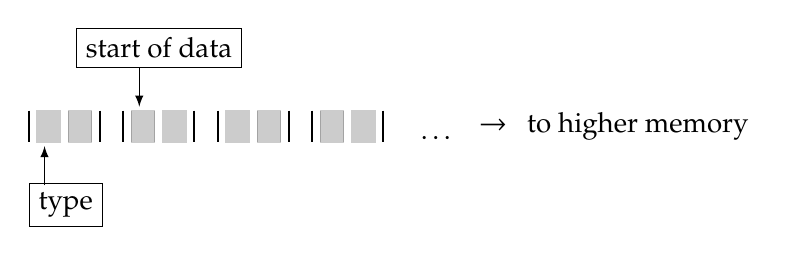
\begin{tikzpicture}
        \foreach \n in {0,...,3}
        {
            \draw [xshift=1.2*\n cm,thick] (0,.4cm)--(0,-.0cm);
            \draw [xshift=1.2*\n cm,fill, opacity=0.2] (+.1,0.4) rectangle (+.4,-.0) {};
            \draw [xshift=1.2*\n cm,fill, opacity=0.2] (+.5,0.4) rectangle (+.8,-.0) {};
            \draw [xshift=1.2*\n cm,thick] (.9,.4cm)--(0.9,-.0cm);
            \coordinate (C\n) at (1.2*\n cm, .2);
        }
        \node[right=1.6cm of C3, anchor=north] (N0) {$\dots$};
        \node[right=2cm of C3] (N1) {$\rightarrow$};
        \node[right=0 of N1] (N2) {to higher memory};
        \node[draw, below= of C0.west,anchor=west] (N3) {type};
        \node[draw, above=1.2cm of C1.west,anchor=west] at (0.6,0) (N4) {start of data};
        \draw[-latex] ($(N4)+(-0.25,-0.25)$) -- ++(0,-.5);
        \draw[-latex] ($(N3.west)+(0.2,0.25)$)  -- ++(0,.5) ;
    \end{tikzpicture}  
    \caption{\textit{Memory structure of a typed scalar}}
    \label{fig:05_01}
\end{figure}
 
We implement a scalar through the defining word

\begin{lstlisting}
    : SCALAR ( type -- )
       CREATE DUP , #BYTES ALLOT
       DOES> DUP@ SWAP 2+ SWAP ; ( -- adr t )
\end{lstlisting}

The word \bc{SCALAR} is used as
\begin{lstlisting}
REAL*4   SCALAR X
REAL*8   SCALAR XX
COMPLEX  SCALAR Z
DCOMPLEX SCALAR ZZ
  etc.
\end{lstlisting}

\subsection{Defining several scalars at once}
\TallC{One} aspect of the FORTH method of handling variables, that seems strange to programmers familiar with Pascal, BASIC, or FORTRAN, is that \bc{VARIABLE}, \bc{CONSTANT} or a new defining word like \bc{SCALAR} need to be repeated for each one defined, as above. That is, such defining words generally do not accept name-lists.

This idiosyncracy can be traced to FORTH's abhorrence of variables:
\begin{itemize}
    \item Easily read (and maintained) FORTH code consists of short definitions with few (generally $\leq$ 4) numbers on the stack. Such programs have small use for variables, especially since the top of the return stack can serve as a local variable.
    \item In FORTH as in BASIC, variables tend to be global and hence corruptible. The variables in a large program can have unmnemonic names or names that do not express their meaning simply because we run out of names.
    \item Experienced FORTH programmers tend to reserve named variables for such special purposes as vectoring execution.
    \item The standard FORTH kernel therefore discourages named variables by making them as tedious as possible.
\end{itemize}

Most objections to variables can be resolved by making them local. Local variables are relatively easy to define in FORTH: a straightforward but cumbersome method for making "headerless" words is given in Kelly's and Spies's book\sepfootnote{05_04}.

HS/FORTH\sepfootnote{05_05} provides beheading in a particularly simple form: \bc{BEHEAD' NAME}, or \bc{BEHEAD" NAME1 NAME2}.

Used after \bc{NAME} has been invoked in the words that need to reference it, \bc{BEHEAD'} removes \bc{NAME}'s dictionary entry leaving pointers and code fields intact and recovering the unused dictionary space. The more powerful word \bc{BEHEAD"} does the same for the range of dictionary entries \bc{NAME1 ... NAME2}, inclusive.

Beheading variable or constant names makes them local to the definitions that use them; they cannot be further accessed --or corrupted-- by later definitions. (Pountain\sepfootnote{05_06} has given yet another method for making variables local, using a syntax derived from "object-oriented" languages such as SMALLTALK.)

Variables are essential for scientific programming. Since we must often have more than two variables, it is silly to repeat \bc{SCALAR}. A simple way to allow \bc{SCALAR} to use a list is

\begin{lstlisting}
    :SCALARS ( n -- )
      SWAP 0 DO DUP SCALAR LOOP DROP ;
    \ Examples:
    \ 2 REAL*4  SCALARS  A  B
    \ 5 COMPLEX SCALARS XA XB XC XD XE
\end{lstlisting}

I find the use of \bc{SCALARS} with modifiers and lists more convenient and readable than many repetitions of \bc{SCALAR}. Its resemblance to FORTRAN (thereby helping me live with my FORTRAN-inspired habits) is pure coincidence. Although possible to use a terminator (",\eg) rather than a count (to define the variable list) I feel it is desirable for the programmer to know how many variable names he has supplied, hence the counted version.

\subsection{Generic access}
\TallC{A} major theme of FORTH is to replace decisions by calculation henever possible\sepfootnote{05_07}. This philosophy usually pays dividends in execution speed and brevity of code.

But there is an even more important reason to avoid \bc{IF ... THEN} decisions, especially when working with modern microprocessors. CPUs like 80x86 and MC680x0 achieve their speed in part by pre-fetching instructions and storing them in a queue in high speed on-chip cache memory. A conditional-branch machine instruction (the crux of \bc{IF ... THEN}) empties the queue whenever the branch is taken. Branches should be avoided because they slow execution far more than one might expect based on their clock-counts alone.

To replace decisions, we use the standard FORTH technique of the execution array (analogous to the familiar assembly language jump table). This lets us compute from the type descriptor which fetch or store to use.

\TallC{We} now define \bc{G@} and \bc{G!} as execution arrays using\sepfootnote{05_08} anexecution-array-defining word \bc{G:}

\begin{lstlisting}
    : G: CREATE ]
       DOES> OVER + + @ EXECUTE ; ( t -- )
    G: G@ R32@ R64@ X@ DX@ ;
    G: G! R32! R64! X! DX! ;
\end{lstlisting}

assembled from components of the FORTH compiler. That is, the ordinary colon \bc{:} might have the high-level definition (shorn of error detection)

\begin{lstlisting}
    : : CREATE ] DOES> @ EXECUTE ;
\end{lstlisting}

\bc{CREATE} makes the new dictionary entry, and \bc{]} switches to
compile mode. \bc{DOES>} specifies the run-time action (recall any word created by \bc{CREATE} leaves its parameter field address
\textbf{-pfa-} on the stack at run-time, \textit{prior} to the actions following \bc{DOES>}). In the case of \bc{:} the run-time action is to fetch the pfa of the new word and execute it. At run-time, words defined using \bc{G:} add twice the type descriptor to the pfa (to get the offset into the array) then fetch the desired address and \bc{EXECUTE} it.

Microprocessors like the MC680x0 and 80386 that can address large, level memories require no further elaboration for \bc{G@} and \bc{G!}. However, if large arrays are to be addressed within the segmented memory addressing protocol of the 8086/80286 chips, we would have to define \bc{G@} and \bc{G!} to use the "far" forms of addressing words\sepfootnote{05_09}. For example, in HS/FORTH such words as \bc{R32@L} expect a segment paragraph number and offset (32 bits total) as the complete address of the variable being fetched to the 87stack. In that case we modify the definition of \bc{SCALAR} to include the segment paragraph number (seg) in the definition (\bc{LISTS} is nonstandard - it is HS/FORTH's name for the portion of the dictionary containing the word headers)

\begin{lstlisting}
    : SCALAR ( type -- )
    CREATE DUP ,        \ make header ,type
    #BYTES ALLOT        \ reserve space
    DOES>  >R
    [ LISTS @ ] LITERAL ( -- seg)
    R@ 2+               ( -- seg off)
    R> @ ;              ( -- seg off type)
    \ Ex: REAL*4 SCALAR X
\end{lstlisting}

\subsection{The intelligent floating point stack (ifstack)}
\TallC{The} \textbf{ifstack} is a more complex data structure than either a simple fstack or the parameter/retum stacks. When a typed datum is placed on the ifstack its type must be placed there also.

But the typed data have varying lengths, from 4 to 16 bytes. We can deal with this two different ways: either \bc{ALLOT} enough memory to hold a stack of the longest type, making each position on the ifstack 18 bytes wide (to hold datum plus type); or manage the ifstack as a modified heap, with the address of a given datum being computable from the ifstack-pointer and the data type.

The 18-byte wide ifstack wastes memory, but is easy to program. (In retrospect, this is exactly the method I used to program adaptive numerical quadrature\sepfootnote{05_10}.) After several false attempts I settled on the fixed-width ifstack. High level FORTH code for this variant is given below.
\begin{multicols}{2}
\begin{lstlisting}[basicstyle=\small,]
\ TYPED DATA STACK MANAGER
TASK FSTACKS
FIND CP@ 0=
?( FLOAD COMPLEX.FTH )

\ define data-type tokens
0 CONSTANT REAL*4
1 CONSTANT REAL*8
2 CONSTANT COMPLEX
3 CONSTANT DCOMPLEX

CREATE #bytes 4 C, 8 C, 16 C,
: #BYTES #bytes + C@ ; 
( type -- length in bytes )

\define scalar and scalars
: SCALAR        ( type -- ) 
    CREATE DUP , #BYTES ALLOT 
    DOES> DUP@ SWAP 2+ SWAP ;

( -- seg off type )
\ say: REAL*4 SCALAR X
: SCALARS ( n type -- )
    SWAP 0 DO DUP SCALAR LOOP
    DROP ;
\ say: 4 DCOMPLEX SCALARS XA XB XC XD

\ definitions for the parallel stack
\ of types and data 
\ Brodle, TF (Brady, NY, 1984) p. 207.

CREATE FSTACK 20 18 * 2+ ALLOT
\ 2 tos-pointer, 20 18-byte cells
: FS.INT FSTACK 0! ;
: EMPTY         ( -- seg off )
    [ LISTS @ ] LITERAL
    FSTACK DUP@ 18 * 2+ + ;
: >FS ( seg off type -- ) \ say: X >FS
    >R >EMPTY ( -- seg off seg' off )
    R@ OVER ! \ store type on ifstack

FS> ( seg off type -- ) \ say: X FS>
FSTACK 1-!              \ dec ifstack ptr
>R >EMPTY               ( -- seg off seg' off' )
DUP@ R@ =               \ srce.type = dest.type ? 
IF 2+ DSWAP             ( -- seg' off' sef off )
R> #BYTES               ( -- seg' off' sef off n )
CMOVEL                  \ move data from ifstack
ELSE RDROP CR 
    ." ATTEMPT TO STORE TO
    WRONG DATA TYPE" ABORT
THEN ;

\ execution-array defining word
\ HS/FORTH has the faster
\ CASE:...;CASE pair for the same job

: G: CREATE ] DOES> OVER + +
    @EXECUTE ; ( t -- )

G: G@ R32@L R64@L X@L DX@L ;
G: G! R32!L R64!L X!L DX!L ;
\ move data from ifstack to/from FPU
: FS>F ( -- t 87: -- x )
    FSTACK 1-!  \ dec ifstack ptr
    >EMPTY      ( -- seg off )
    DUP@ >R 2+
    R@ ( sef off' type )
    G@ R> ;
\ move data from ifstack to 87stack, leave type

:F>FS (t-- 87:x--)
    >R >EMPTY   ( -- sef off )
    R@ OVER !
    2+ R> ;     ( -- sef off' type)
\end{lstlisting}
\end{multicols}
 
The stack comments and comments should make the preceding code self-explanatory.

\subsection{Unary and binary generic operators}
\label{chap:05_02_06}
\TallC{We} want to define generic unary and binary operators whose run-time action selects the desired operation using information contained in the ifstack. A unary operator such as \bc{FNEGATE} or \bc{FEXP} expects one argument and leaves one result. With a floating-point coprocessor (FPU) the only distinction is between real or complex. This distinction is contained in the second bit of the type descriptor, which we exhibit in Table \ref{tbl:05_01} on page \pageref{tbl:05_01}, in binary notation.

Real and complex can then be distinguished \textit{via} the code fragment

\quad 2 AND ( type - - 0 = real$\mid$ 2 = complex )

% Table 5-1
\begin{table}{H!}
    \centering
    \caption{\textit{Bit-patterns of data type descriptors}}
        \bigskip
    \label{tbl:05_01}
    \setlength{\tabcolsep}{30pt}
        \begin{tabular}{|lll|}
            \hline
            & &\\
            \textbf{Type} & \textbf{BINARY} & \textbf{representation} \\
            & &\\
            REAL*4     &  00000000 & 00000000 \\
            & &\\
            REAL*8     &  00000000 & 00000001 \\
            & &\\
            COMPLEX    &  00000000 & 00000010 \\
            & &\\
            DCOMPLEX   &  00000000 & 00000011 \\
            & &\\
            \hline 
        \end{tabular}
\end{table}

Since most unary operators produce results of the same type as their argument, we write a defining word for \textit{generic} unary operators:

\begin{lstlisting}
: GU: CREATE ] DOES>    ( -- pfa )
    FS>F ( -- pfa t )   \ get data
    UNDER 2 AND +       ( -- t adr )
    @ EXECUTE           \ do it
    F>FS ;              \ return ans.
\end{lstlisting}

When we use \bc{GU:} in the form
\begin{lstlisting}
    GU: GNEGATE FNEGATE XNEGATE ;
\end{lstlisting}

\bc{CREATE} produces a dictionary entry for \bc{GNEGATE; ]} turns on the compiler so the previously defined words \bc{FNEGATE} and \bc{XNEGATE} have their addresses compiled into \bc{GNEGATE}'s parameter field; and \bc{DOES>} attaches the run-time code. The run-time code converts the real/complex bit into an offset, 0 or 2 which is added to the address of the daughter word to get the address where the pointer to the actual code is stored. This pointer is fetched and \bc{EXECUTE}d.

A few unary operators like \bc{XABS} (complex absolute value) return real values from complex arguments. If we want to use \bc{GU:} to define, say, \bc{GABS}, we must remember to redefine \bc{XABS} so it zeros the second bit of the type descriptor left on the stack, before returning its result to the ifstack. This is just a \bc{1 AND} so is fast.

% fig. 5-2 
\begin{figure}
    \center
    \newcolumntype{x}[1]{>{\let\newline\\\arraybackslash\hspace{0pt}}p{#1}}
    \setlength{\extrarowheight}{0.1cm}
    \begin{tabular}{|llm{7cm}|}
        \hline
        TYPE\textsubscript{ab} & & \\
        & &
        \begin{tabular}{ x{0.8cm}x{0.8cm} x{0.8cm} x{0.8cm} x{0.8cm} }
            \textsubscript{\space \space b}&&&&\\
            %\textsuperscript{b}&&&&\\
            \diaghead(-3,2){\hskip \hsize} a & R & D & X & DX  \\
            \cline{2-5}
            \multicolumn{1}{ x{0.8cm}|}{R  }&  R & R  & X & X  \\
            \multicolumn{1}{ x{0.8cm}|}{D  }&  R & D  & X & DX \\
            \multicolumn{1}{ x{0.8cm}|}{X  }&  X & X  & X & X  \\
            \multicolumn{1}{ x{0.8cm}|}{DX }&  X & DX & X & DX 
        \end{tabular}
        \\
        & & \\
        \hline
    \end{tabular}
    \caption{\textit{Types resulting from 2-argument operators}}
    \label{fig:F05_02}
\end{figure}

A binary operator (one that takes two arguments) expects its arguments \textit{and} their types on the ifstack. There is no distinction between single- and double-precision arithmetic on most numeric coprocessors. However, the result must leave the proper type-label on the stack. Here is what we want to happen, illustrated in Fig. \ref{fig:F05_02} as a matrix \regc{TYPE(arga, argb))}

\leftbar[1\linewidth]
Note: this protocol avoids misleading precision for the results of computations. It seems more scientific than FORTRAN's "convert intermediate results to the precision of the highest-precision operand" protocol.
\endleftbar

If we think of the indices and entries in Fig. 5-2 as numbers 0, 1, 2, 3 (so we can use them as indices into a table) rather than as letters, a simple algorithm emerges: the first bit of the result is the logical-AND of the first bits of the two operands, and the second bit of the result is the logical-OR of their second bits. Although we would program this in assembler for speed, the high-level definition is

\begin{lstlisting}
: NEW.TYPE  ( a b -- a2 + b2 + a1b1 )
    DDUP        ( -- a b a b        )
    AND         ( -- a b ab         )
    1 AND       ( -- a b [ab]1      )
    -ROT OR     ( -- [ab]1 a+b      )
    2AND        ( -- [ab]1 [a+b]2   )
    + ;         ( -- a2 + b2 + a1b1 )
\end{lstlisting}

Since only logical operations are used, \bc{NEW.TYPE} is faster than table lookup or branching. Note that in programming this key word we have obeyed the central FORTH precept: "Keep it simple!" by choosing a data structure (the numeric type tokens 0-3) that is easily manipulated.

We will also need a way to select the appropriate operator from a jump table of addresses. Given that the precision (internal) is irrelevant, again all that matters is whether the number is real or complex, \ie \,the second bits of the numbers. The first operation must then be to divide by 2 (right-shift by one bit). We then have the matrix of Fig. \ref{fig:05_03} below
% Fig. 5-3 
\begin{figure}[H]
    \center
    \begin{tabular}{|lll|}
        \hline
        && \\
        && \\
        \begin{tabular}{ccc}
            & 0 & 1 \\
            \cline{2-3}
            \multicolumn{1}{c|}{0  }&  RR & RX \\
            \multicolumn{1}{c|}{1  }&  XR & XX \\
        \end{tabular}
        %& $\rightarrow $ &
        & $ \xrightarrow{\hspace*{1cm}} $ &
        \begin{tabular}{ccc}
            & 0 & 1 \\
            \cline{2-3}
            \multicolumn{1}{c|}{0  }&  0 & 1 \\
            \multicolumn{1}{c|}{1  }&  2 & 3 \\
        \end{tabular}
        \\
        &&\\
        &&\\
        \hline
    \end{tabular}
    \caption{\textit{Operator selection matrix}}
    \label{fig:05_03}
\end{figure}
where RR stands for real-real, \textit{etc.} The numerical elements are generated as \regc{2*J+I}. This leads to the word

\begin{lstlisting}
    : WHICH.0P ( a b -- c )
        2/ SWAP 2 AND + ;
\end{lstlisting}

Thus we come to the binary generic-operator defining word
\begin{lstlisting}
    : GB: CREATE ] DOES>        ( -- pfa )
        FS>F FS>F               ( -- pdf t0 t1 )
        NEW.TYPE UNDER          ( -- t' pfa t' )
        WHICH.OP 2* +           \ make result-type
            @ EXECUTE           \ select binop
        F>FS ;                  \ save result
    \say: GB: G*   F*  F*X  X*F  X* ;
\end{lstlisting}

The generic multiply \bc{G*}, \eg, picks out, at run-time, which of four routines to use. By using only logical or shift operations we have made even the high-level definitions fairly quick in comparison with the times of floating point operations.

The only instance where one might forego the overhead penalty paid for the convenience of generic coding would be in nested inner loops, such as occur in matrix operations. Here it might pay to code four inner loops, one for each type, and then access them generically, \eg

\begin{lstlisting}
    : RLOOP      ... real words ...     ;
    : DRLOOP     ... dreal words ...    ;
    : XLOOP      ... complex words ...  ;
    : DXLOOP     ... dcomplex words ... ;
    G: GLOOP  RLOOP DRLOOP XLOOP DXLOOP ;
\end{lstlisting}

\section{Arrays of typed data}

\TallC{Numerical} arrays represent a frequently encountered characteristic feature of scientific programming. Arrays \textit{per se} are hardly foreign to FORTH. Arrays of typed data are novel, however, and therefore worth elaborating. Following Brodie's advice(\TF, p. 48ff) we first specify the "user interface" (matrix notation) and then proceed to implementation.

\subsection{Improved (FORTRAN-like) array notation}
\TallC{Something} like V(15) --the 15'th element of V-- is the commonest notation for array elements in high-level languages because lineprinters and terminals do not easily recognize subscripts. In FORTH, the most natural notation would be postfix (RPN), \bc{15 V} --but this is both hard to read and unintuitive\sepfootnote{05_11}. That is, \bc{15 V} does not say, immediately and unambiguously, "I am the 15th element of the array V !"

FORTH's idiosyncrasies forbid saying V(15) because the parser recognizes V(15) as a single word\sepfootnote{05_12}. Since we want the 15 to be parsed, we would have to modify the FORTRAN-ish notation to $\mathbf V\;\bullet(\;\bullet15)$ or $\mathbf V(\;\bullet15\;\bullet)$, where $\mathbf\bullet$ stands for a blank space (ASCII 32). Unfortunately, "(" is a reserved word. While we might place the matrix definitions in a separate vocabulary --which would let us redefine anything we want-- "(" is too useful as a comment delineator to dispense with.

\TallC{This} leaves the second possibility, where "(" becomes part of the array name, \bc{V(}. To make $\mathbf V(\;\bullet15\;\bullet)$ work,")" must become an operator --unless we want to leave postfix notation entirely, with all the complication \textit{that} would entail\sepfootnote{05_13}. Since ")" is not a reserved word, nothing in principle prevents defining it as an operator. However, such usage would conflict with comments.

The square braces, [ ], are commonly used in matrix notation; however both are reserved FORTH words, \ie\; forbidden. This leaves the curly braces \{ \}, which are unused by FORTH.

Of the two possible forms, $\mathbf V\;\bullet\{\;\bullet15\}$ or $\mathbf V\{\;\bullet15\;\bullet\}$, the latter has the advantage that the opening brace, \bc{\{}, is only part of the name, but reminds us that the name \bc{V\{} \textit{is} an array, exactly as names ending with \bc{\$} are strings, \etc The notation suggests a further mnemonic refinement, namely to place \bc{\{\{} and \bc{\}\}} at the ends of 2-dimensional arrays, as in $\mathbf{M\{\{\bullet \;3 \bullet 5 \;\bullet \}\}}$.

How will this notation operate? Clearly, to place the (generalized) address of the n'th element (of a 1-dimensional array) on the stack we would say

\begin{align*}
    V\{\bullet \;n \;\bullet\}
\end{align*}

whereas

\begin{align*}
    M\{\{ \bullet \;m \bullet n \;\bullet\}\}
\end{align*}

should analogously place the address of the m,n'th element of a 2-dimensional array on the stack.

\subsection{Large matrices}
\TallC{The} defining word \bc{SCALAR} given in \S\ref{sec:Typed_scalars} above allots space in the dictionary --for most FORTHs, code + data must fit here-- or in the LISTS segment of HS/FORTH (part of the dictionary). This is OK for variables, but not for arrays, since even a modest matrix would exhaust the ( $\leq$64 Kbyte) LISTS segment.

A \bc{REAL*4} matrix uses 4 bytes per ellement. The largest such array that can be stored in a 65,536 (\ie, $2^{16}$) -byte segment is 128x128. This is the largest array that can be addressed with unsigned 16-bit numbers. On the other hand, a filled IBM PC/XT clone has 64 Kbytes of memory under MS-DOS. Even a generous F0RTH kernel (plus DOS) takes up less than 150 K; hence 450 K is available to hold large arrays. Up to 8 Mbytes can be added as EMS storage, assuming a suitable memory management scheme\sepfootnote{05_14}. That is, in principle one could tackle matrix problem of order 350x350. What about speed? The dominant term is solving linear equations by --say-- Gaussian elimination with partial pivoting is
\[
T = \frac{1}{3} mn^{3}
\]
where m is the time for 1 multiply and 1 add, and n is the order of the matrix. We should also include the fetch + store time, since the bus bandwidth is as much a limiting factor as the FPU arithmetic speed. For the 8086/8087 the time $m$ is of order 400 clock cycles. Thus the asymptotic execution time on a 10 MHz machine should be of order 10 minutes for n = 350.

On the 80386/80387 combination running at 25 MHz, the execution time for the same problem should be only 2.3 minutes or so. Thus it would be practical (\ie, execution time $\cong$ 1 hour) on such machines, even without special equipment such as the IIT 80c387, or an array co-processor, or a faster procedure such as Strassen's algorithm (see Ch. 4 \S8), to tackle $10^{3} \times 10^{3}$ dense matrix problems.

The crucial question therefore, is memory. The Intel machines were designed around a segmented memory architecture. That is, to avoid having to use (expensive) 32-bit address registers, the 8086/80286 chips were designed to use 16-bit registers. However, these chips have more than 16 external address lines -- 20 for the 8086, 24 for the 80286. Thus the absolute address is compounded of two numbers: a \textbf{segment descriptor} and an \textbf{offset}, which must be present in appropriate registers. The segment descriptor is the \textbf{absolute address} of a l6-byte \textbf{paragraph}, divided by 16. The offset is any (unsigned) integer from 0 to $2^{16}-1 = 65,535$ that can fit in a 16-bit register.

The chips contain 4 segment registers: SS (stack segment), CS (code segment), DS (data segment) and ES (extra segment). Five registers, BP, SP, SI, DI, and BX, can be used for offsets, although they are not entirely interchangeable (some have specific functions in some of the more complex machine instructions, such as string operations). Manifestly, since the 8086 can address

\quad$2^{20} = 1,048,576 \textrm{ bytes ("1 megabyte")}$,

the largest segment number is $2^{14}-1 = 16,383$.

A typical (segmented) address is expressed in Intel assembly code
as

\begin{lstlisting}
    CS: [BX + SI + 0008]
\end{lstlisting}

which translates in words to "add the offset in BX to that in SI and then add 8 to get the total offset; take the segment descriptor in CS, multiply by 16 and add to produce the absolute address\erratumAdd{forgotten word}{"}.

\subsection{Using high memory}
\TallC{HS/FORTH} permits accessing all the memory in a PC/AT (up
to 1 megabyte) in the following manner:
\begin{itemize}
    \item Define a named segment of length 1 byte: this marks the beginning of available memory.
    \item Then tell both FORTH and DOS how much memory you want.
\end{itemize} 

As might be expected, HS/FORTH defines non-standard words (coded as DOS function calls) to use the various DOS service routines that allocate memory, \textit{etc}.\sepfootnote{05_15}

\begin{lstlisting}
    MEMORY 4+ @ S->D
    DCONSTANT MEM.START \ beg. of free memory
    40.960 DCONSTANT MAX.PARS
        \ 40960 = 655360 /16
    : TOTAL.PARS MAX.PARS MEM.START D- ;
        \ # pars of memory available
    1 SEGMENT SUPERSEG
        \ define named segment 1 byte long
    TOTAL.PARS DROP FREE-SIZE
        \ tell DOS and HS/FORTH about it
\end{lstlisting}

Having allocated the memory, how can we address it efficiently? We would like the simplicity of double-length integer arithmetic for computing an (absolute) array address, as in

\begin{lstlisting}
    abs.adr(A_{ij}) = abs.adr(A_{00}) + (row.length*I+J) *#BYTES
\end{lstlisting}

However, although the absolute address referenced by a segment and offset is unique, \ie the absolute address in bytes is

\begin{lstlisting}
    aba.adr = 16*segment + offset ,
\end{lstlisting}

the reverse translation, of an absolute address (in bytes) to the segment + offset notation expected by 80x86 processors is \textit{not} unique. This naturally poses a problem when the processor tries to prevent segments from overlapping (protected mode). In such cases, the only answer is a memory management scheme that computes segments and offsets (by brute force) in a non-overlapping fashion. For example, we might define large arrays such that each row has its own segment paragraph.

The 80386 CPU has a third mode that permits direct 32-bit addressing of 4 gigabytes (albeit few computer users have quite this much fast memory available). A scheme for addressing large amounts of RAM in 80386 machines (without leaving MS-DOS) has been discussed in \textit{Dr Dobb's Journal}\sepfootnote{05_16}.

For 8086 PC's and/or real-mode programming on 80286 + machines, we can merely ignore whether segments overlap. Oddly, standard assembly programming books\sepfootnote{05_17} omit this way of addressing segmented memory.

The 8086 permits 32-bit addressing as long as we translate 32-bit addresses to the segment + offset notation expected by the 80x86 processors in real mode. A word that performs this conversion is \bc{SEG.OFF}, defined as

\begin{lstlisting}
    : >SEG.OFF          ( d -- seg off )
        OVER 15 AND     (   --   d off )
        -ROT D16/ DROP  (   -- off seg )
        SWAP ;
\end{lstlisting}

The 32-bit address is placed on the stack as a double-length integer, with the low-order (\ie\ offset part) above the segment part. The phrase \bc{OVER 15 AND} saves bits 0-3 (of the 32-bit address); \bc{-ROT D/16 DROP} then shifts the (32-bit) address right 4 bits and drops the least-significant part, to produce the offset. This conversion method produces offsets in the range 00-0F (hex), that clearly have nothing to do with the original offsets (that led to the 32-bit absolute address \textit{via} 16*seg + off ).

\subsection{A general typed-array definition}
\TallC{For} the new syntax to work the word \bc{\}} must compute the addresses of the n'th element of \bc{V\{} from the information on the stack, and \bc{\}\}} must do the same for \bc{M\{\{}. In order to encompass matrices of typed data we specify that the results of the phrases \bc{V\{ n \}}and \bc{M\{\{ m n \}\}} be to leave the generalized address on the parameter stack, \ie to leave the stack picture \regc{( -- seg off type)}, exactly as with \bc{SCALAR}s.

Before we can define \bc{\}}, however, we must specify the data: structure it operates on, \ie\ the array header.

Once again we begin with the user interface. We can opt for maximum generality or maximum simplicity. My first attempt fell into the first category, permitting the user to define a named segment of given length and to define an array in that segment. Lately I realized this generality accomplishes little, so have abandoned it. All arrays will be defined in the heap, named \bc{SUPERSEG} as above. To define a length-50 \bc{1ARRAY} of 4-byte number we will say

\begin{lstlisting}
    50 LONG REAL*4 1ARRAY V{
\end{lstlisting}

Now, before we work out the mechanics of \bc{1ARRAY}, we imagine that an array will be stored as in Fig. \ref{fig:05_04} below:

The proposed data structure consists of an 8-byte header (the \textbf{array descriptor}) in the dictionary (\regc{LISTS} in HS/FORTH), with the \textbf{body} of the array stored elsewhere. The array descriptor points to the absolute address of the array data (body).
% Fig. 5-4 
\begin{figure}
    \center
    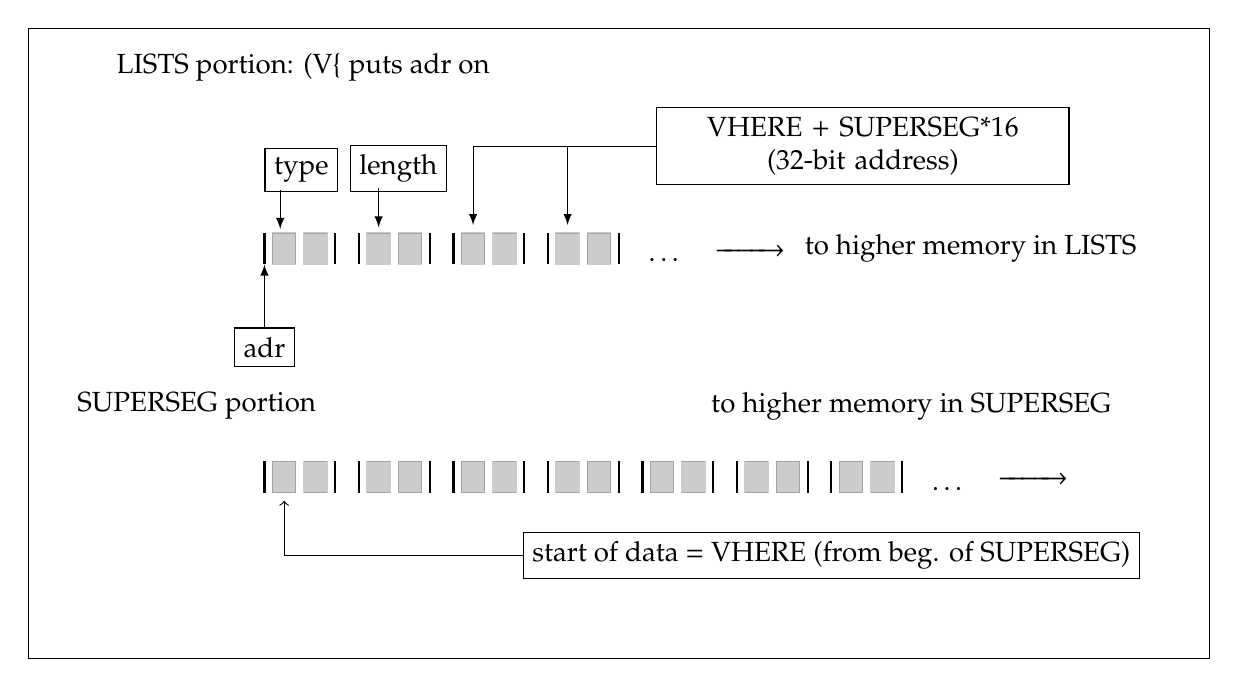
\begin{tikzpicture}
        \draw (-3,-5) rectangle (12,3.0);
        \node[align=left, anchor=west] at (-2,2.5) {LISTS portion: (V\{ puts adr on};
        \node[align=left, anchor=west] at (-2.5,-1.8) {SUPERSEG portion};
        \foreach \n in {0,...,3}
        {
            \draw [xshift=1.2*\n cm,thick] (0,.4cm)--(0,-.0cm);
            \draw [xshift=1.2*\n cm,fill, opacity=0.2] (+.1,0.4) rectangle (+.4,-.0) {};
            \draw [xshift=1.2*\n cm,fill, opacity=0.2] (+.5,0.4) rectangle (+.8,-.0) {};
            \draw [xshift=1.2*\n cm,thick] (.9,.4cm)--(0.9,-.0cm);
            \coordinate (C\n) at (1.2*\n cm, .2);
            \coordinate (CB\n) at (1.2*\n cm, 0);
            \coordinate (CT\n) at (1.2*\n cm, 0.4);
            \coordinate (FT\n) at (1.2*\n +0.25, 0.5);
            \coordinate (ST\n) at (1.2*\n +0.5, 0.5);
        }
        \node[right=1.5cm of C3, anchor=north] (N0) {$\dots$};
        \node[right=2cm of C3] (N1) {$\xrightarrow{\hspace*{0.7cm}}$};
        \node[right=0 of N1] (N2) {to higher memory in LISTS};
        \node[draw, above= of C0.west,anchor=west] (N3) {type};
        \node[draw, above= of ST2] at (1.7,-0.08) (N4) {length};
        \node[draw, below= of C0.west] (N5) {adr};
        \node[align=center, draw, text width=5cm] at (7.6,1.5) (N6) {VHERE + SUPERSEG*16\\(32-bit address)};
        \draw[-latex] ($(N4)+(-0.25,-0.25)$) -- ++(0,-.5);
        \draw[-latex] ($(N3.west)+(0.2,-0.25)$)  -- ++(0,-.5) ;
        \draw[-latex] (N5.north)  -| (CB0) ;
        \draw[-latex] (N6.west)  -| (FT3) ;
        \draw[-latex] (N6.west)  -| (FT2) ;

        \foreach \n in {0,...,6}
        {
            \draw [yshift=-2.9cm, xshift=1.2*\n cm,thick] (0,.4cm)--(0,-.0cm);
            \draw [yshift=-2.9cm, xshift=1.2*\n cm,fill, opacity=0.2] (+.1,0.4) rectangle (+.4,-.0) {};
            \draw [yshift=-2.9cm, xshift=1.2*\n cm,fill, opacity=0.2] (+.5,0.4) rectangle (+.8,-.0) {};
            \draw [yshift=-2.9cm, xshift=1.2*\n cm,thick] (.9,.4cm)--(0.9,-.0cm);
            \coordinate (C\n) at (1.2*\n, -2.9+0.2);
            \coordinate (FB\n) at (1.2*\n +0.25, -2.9 -0.1);
            \coordinate (st\n) at (1.2*\n +0.75, -2.9 +0.5);
        }
        \node[right=1.5cm of C6, anchor=north] (n0) {$\dots$};
        \node[right=2cm of C6] (n1) {$\xrightarrow{\hspace*{0.7cm}}$};
        \node[draw, below=0.7cm of C6] (n3) {start of data = VHERE (from beg. of SUPERSEG)};
        \draw[->] (n3.west) -| (FB0);
        \node[above=0.6cm of st4, anchor=west] (n2) {to higher memory in SUPERSEG};
    \end{tikzpicture} 
    \label{fig:05_04}
    \caption{\textit{Structure of a 1-dimenslonal array in \regc{SUPERSEG}}}
\end{figure}

The array-defining word \bc{1ARRAY} must perform the following
tasks:

\begin{itemize}
    \item place the length and type of the data in the first two cells (4 bytes) of the array descriptor.
    \item place the 32-bit address (start of data) in the next two cells (4 bytes) of the array descriptor.
    \item allot the necessary storage in \bc{SUPERSEG}.
    \item at run-time, place the generalized address, length and type on the parameter stack.
\end{itemize}

The start of data is handled by \bc{VHERE}, a word that puts the next vacant (32-bit) address in \bc{SUPERSEG} on TOS.

We define \bc{VALLOT} to keep track of the storage used by arrays. \bc{VALLOT} increments the pointer in \bc{VHERE} (and aborts with a warning if the segment length is exceeded).

We first define some auxiliary words:
\begin{lstlisting}
    MEMORY 4 + @
    S-> D DCONSTANT MEM.START
        \ beg. of free memory
    40.960 DCONSTANT MAX.PARS \ 40960 = 655360/16
    : TOTAL.PARS MAX.PARS   MEM.START D- ;
        \ # pars avail. mem.
    1 SEGMENT SUPERSEG        \ named seg. 1 byte long
    TOTAL.PARS DROP
        FREE-SIZE             \ tell DOS and HS/FORTH

    DVARIABLE VHERE>
    : INIT.VHERE> 0.0 VHERE> D! ;
    INIT.VHERE>
    : VHERE ( -- d.offset ) VHERE> D@ ;
    : D4/   D2/ D2/ ;
    : D16/  D4/ D4/ ;

    : TOO-BIG? VHERE >SEG.OFF
        0 AND TOTAL.PARS D>
        ABORT" INSUFFICIENT ROOM IN SUPERSEG" ;
        \ check whether new value of VHERE> passes end
        \ of SUPERSEG

    : VALLOT ( d.#bytes -- )
        VHERE  D+ DDUP TOO.BIG?
        VHERE> D! ;

    \ Array-defining words
    \ Ex: 50 LONG REAL*4 1ARRAY V{
    \ V{            (   -- adr )
    \ V{ 17 } >FS   (:: -- V[17])

    : LONG DUP ;
    FIND D, 0= ?( :D, SWAP , , ; )
        \ conditionally compile D,
    :1ARRAY ( I I t -- )
        CREATE UNDER D,  \ t,I into 1st 4 bytes { -- I t )
        SUPERSEG @ 16 M* \ start of SUPERSEG
        VHERE D+ D,      \ abs. address -> next 4 bytes
        #BYTES M*        ( I t -- #bytes to allot)
        VALLOT ;         \ allot space in the segment
    \ run-time action: ( -- adr )
\end{lstlisting}

We also need some words to go with \bc{1ARRAY}:
\begin{lstlisting}
    : } (adr n -- seg.off[n] t )
        SWAP DUP@ R > \ type -> rstack
        4+  D@
        ROT R@ #BYTES M*
        D+ >SEG.OFF R > ; ( -- seg.off[n] t )
\end{lstlisting}

Finally, here is a useful diagnostic word

\begin{lstlisting}
    :7TYPE ( t-- ) \ it's ok for this to be slow!
        DUP 0 = IF DROP ." REAL*4"   EXIT THEN
        DUP 1 = IF DROP ." REAL*8"   EXIT THEN
        DUP 2 = IF DROP ." COMPLEX"  EXIT THEN
        DUP 3 = IF DROP ." DCOMPLEX" EXIT THEN
        ." NOT A DEfiNED DATA TYPE" ABORT ;
\end{lstlisting}

\subsection{2ARRAY and \}\} }
\TallC{We} now want to define arrays of higher dimensionality. For example, to define a 2-dimensional array we might say

\begin{lstlisting}
    90 LONG BY 90 WIDE COMPLEX 2ARRAY XA{{
\end{lstlisting}

This leads to the definitions
\begin{lstlisting}
    : BY ; \a do-nothing word for style
    : WIDE * ; (I w -- I*w)
    : 2ARRAY   (I*w t -- ) 1ARRAY ;
\end{lstlisting}

Now let us define \bc{\}\}} to fetch the double-indexed address:

\begin{lstlisting}
    : }} ( adr m n -- a[m*I+n] t)
        >R OVER 2+ @ ( -- adr m I*w)
        * R> + } ;
\end{lstlisting}

By correct factoring (putting some of the work into \bc{WIDE}) we achieved an easy definition of \bc{2ARRAY}. Careful factoring also let
us define \}\} in terms of \}.

\section{Tuning for speed}

\TallC{Some} of the words in our typed-data/matrix lexicons should be optimized or redefined in machine code. Accessing matrix elements imposes a non-trivial overhead on matrix operations. We can reduce the execution time with inline code, either in the traditional FORTH manner \textit{via} selected assembler definitions, or with a recursive-descent optimizer such as HS/FORTH's\sepfootnote{05_18}.

Experience teaches that optimization is most fruitful (most bang for the buck) applied to entire inner loops and other selected areas of code, rather than to access words \textit{per se}. By hand-coding the innermost loop in matrix inversion and FFT routines, one achieves programs that run in (asymptotically) minimum time on the 8086/8087 chip set.

\TallC{Significant} speed increases in data access could perhaps be obtained with multiple code field (MCF) words, as described by Shaw\sepfootnote{05_19}, and as implemented by HS/FORTH in the words \bc{VAR}, \bc{AT}, \bc{IS}, and variants thereof. The disadvantage of MCF style is that compile-time binding, while faster in execution, loses the flexibility of run-time binding. That is, data types would --as with FORTRAN-- be specified at compile-time, and lexicons would be recompiled to run with specific types. Run-time binding as described in this Chapter produces \textit{generic} words that can handle all four standard scientific data types, a major advantage over MCF.
\\
\leftbar[1\linewidth]
FORTH data structures, especially as defined in this Chapter, do little-- or no bounds checking, hence do not prevent accidentally overwriting key parts of the operating system.

The new fetch and store words were defined in high-level FORTH for safety. Adding bounds-checking to arrays, at least during the debug cycle, is \underline{strongly recommended} to avoid crashing, or even damaging, the system.
\endleftbar
        % % Chapter 6 -- Programming Examples

\chapter{Programming Examples}

\TallC{This} chapter illustrates how we may apply the floating point extensions of FORTH, developed in preceding chapters, to some standard problems in numerical analysis.

\section{Infinite series}
\TallC{Frequently} we must evaluate a function defined by an infinite sum

\begin{align}
    f(x) = \sum_{n=0}^{\infty}c_{n}x^{n}
    \label{eq:06_01}
\end{align}

where $x$ is a real number and $c_n$ is an infinite sequence of coefficients. The extensive mathematical theory\sepfootnote{06_01} of such functions can be summarized as follows: the series of terms only have meaning if --for fixed $x$-- the sequence of partial sums

\begin{align}
    f_{N}(x) = \sum_{n=0}^{N-1}c_{n}x^{x}
\end{align}

has a definite limit.

\subsection{Examples of Infinite series}
\TallC{Perhaps} the formal definitions will seem clearer after some concrete examples. We now examine some divergent and convergent series.

\subsubsection{Divergent examples}
What does it mean to say a series diverges? Consider the series whose terms are all 1's (that is, $c_n = 1, x = 1$):

\begin{align}
    1 + 1 + 1 + 1 + ...
\end{align}

The partial sum $f_N$ is just $N$, and therefore increases without limit as more terms are added. The series \textit{diverges}.

A harder case is the series whose terms are alternately 1's and -1's:

\begin{align}
    1 - 1 + 1 - 1 + 1 - ...
\end{align}

Depending on how the terms are grouped together, the partial
sums can have any value. Certainly the partial sums do not settle
down to any definite value. The series \textit{diverges}.

Yet a third case is the harmonic series

\begin{align}
    f_{N} = 1 + \frac{1}{2} + \frac{1}{3} + \frac{1}{4} + ... + \frac{1}{N}
\end{align}

It can be shown that for large $N$, $f_{N}$ is approximately $log_{e}(N)$, so the harmonic series \textit{diverges}.

\subsubsection{A convergent example}
Are there ever mes of infinite series that \textit{do} mean something? Obviously, or there could hardly be a theory of them! An example\sepfootnote{06_02} is $c_{n}=1, x = \frac{1}{2}$. Here the partial sums
\begin{equation}
\begin{aligned}
f_{0} &= 1                               \\
f_{1} &= 1 + \frac{1}{2}                 \\
f_{2} &= 1 + \frac{1}{2} + \frac{1}{4}   \\
...&.....................                \\
\lim_{N\to\infty} f_{N} &\equiv \lim_{N\to\infty} \frac{1-(\frac{1}{2})^{N}}{1-\frac{1}{2}} = 2
    \label{eq:06_06}
\end{aligned}
\end{equation}
\textit{do} have a definite limit, so the series converges.

\subsection{Numerical examples of convergent series}
\TallC{How} do we tell whether a series has converged? As a practice matter, we keep adding terms to the partial sum until it no longer changes, within the desired precision. Sometimes this can involve a great many terms, even when the series converges. There exists an extensive mathematical literature on testing for the convergence of an infinite series. Mathematicians have also developed many tricks for accelerating the convergence of slowly converging series\sepfootnote{06_03}. Consulting the literature in difficult cases is strongly recommended -- it can save time galore!

As an heuristic exercise, let us write some simple programs to evaluate partial sums and see how convergence works.

First we sum the terms $2^{-n}$ from Eq. \ref{eq:06_06}. The flow diagram is shown in Fig. \ref{fig:06_01} below.

%\tikzstyle{line} = [draw, -latex']
\tikzset{%
  do path picture/.style={%
    path picture={%
      \pgfpointdiff{\pgfpointanchor{path picture bounding box}{south west}}%
        {\pgfpointanchor{path picture bounding box}{north east}}%
      \pgfgetlastxy\x\y%
      \tikzset{x=\x/2,y=\y/2}%
      #1
    }
  },
  cross/.style={do path picture={    
    \draw [draw, -latex', cap=round] (-1,-1) -- (1,1) (-1,1) -- (1,-1);
  }},
  dot/.style={do path picture={    
    \draw [fill]  circle [radius=1]; 
  }}
}
\begin{figure}
% Fig. 6-1 
    \begin{tikzpicture}[minimum size=0.75cm]
        \draw (8,0.5) -- (-4, 0.5) -| (-4,-10) |- (8,-10);
        \node (start) {};
        \node [circle, draw, cross, below=0.5cm of start] (cross) {};
        \node [right=of cross, xshift=-0.5cm] (cyc) {BEGIN} ;
        \node [above =1.0cm of cyc.west,anchor=west] {SET UP: \space N=0 \space SUM=1};
        \node [below=1.5cm of cyc.west, anchor=west, align=left, text width=6cm, xshift=-0.5cm] {?CONTINUE ( 10 or more terms? )\\WHILE} ;
        \node [below= of cross] (cond) {};
        \node [circle, draw, cross, below= of cond] (cross2) {};
        \node [circle, draw, dot, below=1.6cm of cross2] (dot1)  {};
        \node [circle, draw, dot, below= of dot1] (dot2)  {};
        \node [left=of cond] (NO) {};
        \node [draw, fill, opacity=0.2, below= of NO, text width=1.2cm]  (ext) {};
        \draw [->] (start) -- (cross);
        \draw [->] (cross) -- (cond.mid);
        \draw [->] (cond.mid) -- (cross2);
        \draw [->] (cross2) -- (dot1);
        \draw [->] (dot1) -- (dot2);
        \draw [->] (cond.mid) -- (NO.mid);
        \draw [->] (NO.mid) -- (ext);
        \node [right=of dot1, align=left, xshift=-0.5cm] {LOOP} ;
        \node [right=of dot2, align=left, xshift=-0.5cm] {REPEAT} ;

        \node [right= of cross2, align=left, xshift=-0.5cm] (lp0) {10 \space 0 \space DO} ;
        \node [below=.5cm of lp0.mid,anchor=west, align=left, xshift=-0.3cm] (lp1) {$2^{-n-1}=2^{-n}/2$} ;
        \node [below=.5cm of lp1.west,anchor=west, align=left] (lp2) {SUM = SUM + $2^{-n-1}$} ;
        \node [below=.5cm of lp2.west,anchor=west, align=left] (lp3) {n = n + 1} ;
        \node [left=.1cm of cond.south, align=left] (TYES) {YES} ;
        \node [left=.1cm of NO.south, align=left] (TNO) {NO} ;
        \node [below=-0.1cm of ext.south, align=left] (TEXIT) {Exit} ;
    \end{tikzpicture}
    \caption{\textit{Computing 2 the hard way}}
    \label{fig:06_01}
\end{figure}

The corresponding program is

\begin{lstlisting}
    15 #PLACES !            \ set F. to 15 digits
    : NEXT.TERM
        ( n -- n+1 :: sum 2^-n -- sum' 2^-n-1 )
        F2/ FUNDER F+ FSWAP 1+ ;
    : SET.UP FINIT F=1 F=1 0 ;
    : EXHIBIT CR DUP ." n = " .
        2 SPACES
        FOVER ." sum = " F. ;
    : ?CONTINUE  CR ." Another 10 terms?" ?YN ;
    \ ?YN expects a "y" or "n" from the keyboard and
    \ leaves -1 ("true") if "y" is pressed, 0 if "n"
    : SUM SETUP
        BEGIN EXHIBIT ?CONTINUE
        WHILE 10 0 DO NEXT.TERM LOOP
        REPEAT ;
\end{lstlisting}

This is what a run looks like:

\begin{lstlisting}
    FLOAD TEST.SUM Loading TEST.SUM ok
    SUM
    n = 0  sum = 1.00000000000000
    Another 10 terms? Y
    n = 10 sum = 1.919902343750000
    Another 10 terms? Y
    n = 20 sum = 1.99999904632568
    Another 10 terms? Y
    n = 30 sum = 1.99999999906867
    Another 10 terms? Y
    n = 40 sum = 1.99999999999909
    Another 10 terms? N ok
\end{lstlisting}

The partial sums converge rapidly to 2 (which, as we saw in \S \ref{sec:01_01_02} above, is the exact sum).

For a second example, let us sum a standard infinite series representation for $\pi/4$: We note that the function $\tan^{-1}(x)$(that is, arctan(x) ) has the infinite series representation\sepfootnote{06_04}

\begin{align}
    \tan^{-1}(x) = x - \frac{x^{3}}{3} + \frac{x^{5}}{5} - \frac{x^{7}}{7} ...
    \label{eq:06_07}
\end{align}

Since a 45$^{\circ}$ right triangle has equal height and base, the tangent of 45$^{\circ}$ is 1 (side opposite over side adjacent). That is\sepfootnote{06_05},
\begin{align}
    \frac{\pi}{4} \equiv \tan^{-1}(1) = 1 - \frac{1}{3} + \frac{1}{5} - \frac{1}{7} + \frac{1}{9}...
    \label{eq:06_08}
\end{align}

Actually the series Eq. \ref{eq:06_08} is slowly converging and therefore a poor way to compute $\pi$\sepfootnote{06_06}. But anyway, let us proceed. The flow diagram is now that of Fig. \ref{fig:06_02} below.

% Fig. 6-2 
\begin{figure}
    \begin{tikzpicture}[minimum size=0.5cm]
        \draw (-2, 0.5) rectangle (10,-7);
        \node (start) {};
        \node [circle, draw, cross, below=0.5cm of start] (cross) {};
        \node [below=0.5cm of cross] (cond) {};
        \node [circle, draw, dot, below right= 4.5cm and 2cm of cross] (dot1)  {};
        \node [left=of cond] (NO) {};
        \node [draw, fill, opacity=0.2, below= 1.5cm of NO, text width=1.2cm,xshift=.8cm]  (ext) {};
        \draw [->] (start.mid) -- (cross);
        \draw [->] (cross) -- (cond.mid) -- ++(-.75, -0.75) -- (ext);
        \draw [->] (cond.mid) -| (dot1);
        \node [right=of dot1, align=left, xshift=-0.8cm, yshift=0.25cm] {REPEAT} ;

        \node [below=-0.1cm of ext.south, align=left] (TEXIT) {Exit} ;
        \node [right=of cross, xshift= 1.5cm] (cyc) {BEGIN} ;
        \node [above =1.0cm of cyc.west,anchor=west] {SETUP: flag=1 n=1 sum=0 ( -\phantom{}- 1 n :: -\phantom{}-0)};
        \node [below=1.3cm of cyc.west, anchor=west, align=left, text width=6.5cm, xshift= 0.5cm] (blob) {
            EXHIBIT \hspace{0.6cm} \textbackslash \space display n, sum \\
            ?CONTINUE  \space \space \space WHILE \\
                \leavevmode    \\
            DUP S-\textgreater F  \space 1/F  \space   ( -\phantom{}- f n :: -\phantom{}- sum 1/n ) \\
            SWAP FDUP FSIGN \textbackslash \space transfer sign\\
        };
        \node [below=1.7cm of blob.west, anchor=west, align=left, text width=7cm, xshift= -0.2cm] {
            F+  
            \hspace{3.2cm}
            \textbackslash  \space sum = sum +\\ 
            term\\
            NEGATE  \hspace{2.0cm}  \textbackslash  \space flip sign of f
        };
    \end{tikzpicture}
    \caption{\textit{Computing $\pi/4$ by the infinite series for $\tan^{-1}(1)$}}
    \label{fig:06_02}
\end{figure}


The corresponding program is
\begin{lstlisting}
    15 #PIACES ! \ set F. to 15 digits
    : NEXT.TERM ( f 2n+1 -- f' 2n+3 :: sum -- sum' )
        DUP S->F 1/F SWAP DUP FSIGN F+
        NEGATE SWAP 2+ ;
    : SETUP FINIT F=0 1 1 ;
    : EXHIBIT CR DUP
        ." n = " . 2 SPACES
        FDUP F2* F2* ." 4*sum = " F. ;
    : ?CONTINUE ." Another term?" ?YN ;

    : PI/4 SET.UP
        BEGIN EXHIBIT
        ?CONTINUE
        WHILE NEXT.TERM REPEAT ;
\end{lstlisting}

Now we run the program\sepfootnote{06_07}:

\begin{lstlisting}
    FLOAD PIBY4 Loading PIBY4 ok
    PI/4
\end{lstlisting}
\begin{multicols}{2}
\begin{lstlisting}[basicstyle=\tiny,]
n = 1  4*num = 0.00000000000000 Another term? Y
n = 3  4*num = 4.00000000000000 Another term? Y
n = 5  4*num = 2.66666666666666 Another term? Y
n = 7  4*num = 3.66666666666666 Another term? Y
n = 9  4*num = 2.89523809523809 Another term? Y
n = 11 4*num = 3.33968253968253 Another term? Y
n = 13 4*num = 2.97604617604617 Another term? Y
n = 15 4*num = 3.28373848373848 Another term? Y
n = 17 4*num = 3.01707181707181 Another term? Y
n = 19 4*num = 3.25236593471887 Another term? Y
n = 21 4*num = 3.04183961892940 Another term? Y
n = 23 4*num = 3.23231580940559 Another term? Y

n = 25 4*num = 3.05840276592733 Another term? Y
n = 27 4*num = 3.21840276592733 Another term? Y
n = 29 4*num = 3.07025461777918 Another term? Y
n = 31 4*num = 3.20818565226194 Another term? Y
n = 33 4*num = 3.07915339419742 Another term? Y
n = 35 4*num = 3.20036551540954 Another term? Y
n = 37 4*num = 3.08607980112383 Another term? Y
n = 39 4*num = 3.19418790923194 Another term? Y
n = 41 4*num = 3.09162380666783 Another term? Y
n = 43 4*num = 3.18918478227759 Another term? Y
n = 45 4*num = 3.09616152646364 Another term? Y
n = 47 4*num = 3.18505041535253 Another term? N ok
\end{lstlisting}
\end{multicols}

The first thing we notice is that the numbers seem to be converging to \textit{something}; however, unlike the previous series, the differences between successive partial sums are fairly large.

An infinite series of terms that alternate in sign and decrease in magnitude is guaranteed to converge\sepfootnote{06_08}. The error (that is, the difference between a partial sum and the limit) is of the order of the first neglected term and has the same sign. We see that for this case, the error in computing $\pi$ is of order $2/n$, where $n$ is the number of terms in the sum. To get $\pi$ to 3 significant figures, therefore, we need about 1000 terms! This is why the series representation for $4\tan^{-1}{(1)}$ is not a very good way to calculate $\pi$. A better way uses \eg,
\begin{align*}
    \pi = 16\tan^{-1}\left ( \frac{1}{5}\right ) - 4\tan^{-1}\left(\frac{1}{239}\right) ,
\end{align*}
which converges much faster\sepfootnote{06_09}.

\subsection{The infinite sum program}
\TallC{Evaluating} a function from its infinite series representation Eq. \ref{eq:06_01} provides an illustration both of indefinite loops and of tests of floating point numbers. We anticipate a program structure something like this:

\begin{lstlisting}
    BEGIN
      Calculate next term
      Not converged?
    WHILE
      Update:
        Add next term to sum
        increment n
    REPEAT
\end{lstlisting}

To actually write the program, we begin at the end, by specifying how we want to invoke the function.

Functions in the standard FORTH library (Ch. 3\S\ref{sec:03_03}) typically expect a single real number on the fstack replacing it with the function: $x \rightarrow f(x)$. Since the sum is infinite, we supply the coeifcients $c_n$ as a function of $n$ rather than as an array. For any given $c_n=f(n)$, it is easy enough to write a FORTH word that evaluates it and leaves the result on the appropriate stack (87stack, fstack, ifstack). For example, to evaluate the exponential \textit{via} the power series

\begin{align}
e^x = 1 + \frac{x^1}{1!} + \frac{x^2}{2!} + \frac{x^3}{3!} + ...
\end{align}

we would define the word NEXT.TERM as

\begin{lstlisting}
    : NEXT.TERM ( 87: term x n -- term*x/[n+1] x n+1 )
        F=1 F+ \ n-> n+1
        FROT FOVER F/ ( 87: -- x n+1 term/[n+1])
        FROT FUNDER F* F-ROT ;
\end{lstlisting}

\subsubsection{Function calls In FORTRAN}
However, FORTRAN (as well as languages that emulate it) achieves readability by passing arguments to functions in a list. In fact, function names can also be passed in the argument list. Thus, \eg, a general FORTRAN program to evaluate a function by summing an infinite series could be written

\begin{lstlisting}
    REAL FUNCTION XINFSUM(X, E, C)
C
C   EVALUATE INFINITE POWER SERIES
C
    EXIERNAL C
    REAL X, E, C
    SUM  = 0
    TERM = 1
    N = 1
1   SUM  = SUM + TERM
    TERM = TERM*X*C(N)
    N = N + 1
    IF (TERM .LE. E) RETURN
    GOTO 1
    END
\end{lstlisting}

where the program to evaluate the exponential would be

\begin{lstlisting}
REAL FUNCTION EXP(x)
EXTERNAL XINFSUM, COEFEXP
REAL C0, XINFSUM
COMMON /CBLK/C0
C0 = 1
EXP = XINFSUM(X, 1.E-7, C0EFEXP)
RETURN
END
\end{lstlisting}

given the coefficient function

\begin{lstlisting}
REAL FUNCTION OOEFEXP(N)
COMMON /CBLK/C0
C0 = C0/N
COEFEXP = C0
RETURN
END
\end{lstlisting}

\subsubsection{A function protocol for FORTH}\label{chap:06_03_02}

We would like to extend to FORTH FORTRAN's ability to write a generic series summation function, passing the variable and the name of the coefficient function as arguments. In other words, we now face the task of devising the function protocol we plan to use throughout the rest of the book and in our future programming -- a heavy responsibility since we do not know what form these future programs will take. \textbf{For once we must engage in top-dawn programming!}

We want our protocol to have several features:
\begin{itemize}
    \item It must be \textbf{telegraphic}, \ie\ it must immediately suggest what it is doing -- a matter of choosing good names.
    \item It must be \textbf{simple} to implement and easy to remember -- the advantages of using it must not be outweighed by complexity.
    \item It must be \textbf{fast} -- a major drawback to FORTRAN's way of doing things is the overhead in function calls.
    \item It must be \textbf{portable} -- it cannot depend on specific details of the FORTH implementation or the machine it is running on.
\end{itemize}

It is simpler to thread this particular maze in reverse: begin with where we want to end up, and determine what steps got us there. We suppose we have defined a generic power series summation function, using the ifstack defined in Ch. 5\S\ref{sec:05_02_05}:
\begin{lstlisting}
    : SUMPOWERS       ( 87: err -- :: x -- sum )
    E G!              \ store error
    FS>F DUP F>FS     \ get type of x
        DUP G=1       \ x**0
    G=0 0 DUP         ( -- n=0 :: -- x 1 0 )
    adr.c EXECUTE G+  ( -- 0   :: -- x 1 c[0] )
    BEGIN 1+          ( -- n   :: -- x x**n-1 sum )
    FS>F GOVER G*
        ( -- n 87: -- sum :: -- x x**n)
    DUP adr.c EXECUTE
        ( -- n :: -- x x**n )
    3 GPICK G* F>FS
        ( -- n :: -- x x**n term sum )
    ENUF? NOT WHILE
        G+
    REPEAT G+ CLEANUP ;
\end{lstlisting}

The words \bc{E}, \bc{ENUF?} and \bc{CLEANUP} have straightforward definitions with obvious meanings; \bc{adr.c} has not been defined because we have yet to figure out what it will do.

Manifestly, \bc{adr.c} must place the execution address ("code-field address" -- \textbf{cfa}) on the stack for \bc{EXECUTE} to find. There are several ways to accomplish this. Clearly, we want to keep the variable that holds the cfa local, so it will not get confused with another function's cfa. While it is straightforward to define a variable and then make it headerless --hence local-- (\textit{via} \bc{BEHEAD"}, \eg) we would prefer to avoid defining a variable at all. Here is a perfect opportunity to use the \textbf{return stack} (rstack).

We imagine that \bc{SUM.POWERS} expects the cfa of the function $c_n$ on the stack. Then the first thing \bc{SUM.POWERS} must do is stash the cfa somewhere convenient but local. One such place is the stack itself. Even easier, since \bc{SUM.POWERS} does not use the rstack explicitly (\eg in a \bc{DO ... LOOP}), is to let the first step in \bc{SUM.POWERS} be \bc{>$R}. Then the code for \bc{adr.c} would be merely \bc{R@}. The final word, after invoking \bc{CLEAN.UP} (that drops unwanted items from the various stacks), then must be \bc{RDROP} (for systems without it, \bc{: RDROP R$>$ DROP ;} ).

The revised version of \bc{SUM.POWERS} is then
\begin{lstlisting}
: SUM.POWERS    ( adr.c -- 87: err -- :: x -- sum )
    > R             \ adr.c -> rstack
    E G!            \ store error
    FS>F  DUP F>FS  \ get x's type
          DUP G=1   \ x**0
    G=0 0 DUP       ( -- n=0 :: -- x 1 0 )
    R@ EXECUTE G+   ( -- 0   :: -- x 1 c[0] )
    BEGIN 1+        ( -- n   :: -- x x**n-1 sum )
       FS>F GOVER G*   ( -- n 87: -- sum :: -- x x**r )
       DUP R@ EXECUTE  ( -- n:: -- x x**n c[n] )
       3 GPICK G* F>FS ( -- n:: -- x x**n term sum )
       GOVER
    ENUF? NOT   WHILE G+ REPEAT
    G+ CLEAN.UP RDROP ;
\end{lstlisting}

The full program to evaluate the exponential by summing power series would then have the form shown below:

\begin{multicols}{2}
\begin{lstlisting}[basicstyle=\scriptsize,]
\ evaluate exponential by summing series
REAL*4 SCALAR E
: ENUF? (::term--) (--F)
    GABS FS>F EG@ F> ;
: CLEAN.UP ( n -- ::x x**n sum -- sum )
    DROP FS >F
    GDROP GDROP F>FS ;
\ definition of SUM.POWERS from above
BEHEAD" E CLEAN.UP \ hide these def'ns
REAL*8 SCALAR c F=1 c G!
: COEEEXP (n--) (:: -- c[n] )
    DUP 1 < =
    IF F=1 c G! F=1 DROP
    ELSE c G@ S->F
        F* FDUP c G! 1/F
    THEN REAL*4 F>FS ;
BEHEAD' c \ hide this variahie
: USE( [COMPILE] ' CFA LITERAL ;
    IMMEDIATE
\ this means "use address of"
\ --crucial def'n of function lexicon
:E**X (::x--e**x) %1.E-8
            \ error on 87stack
    USE( COEFF.EXP
            \ adr.c on stack
    SUMPOWERS ;
\end{lstlisting}
\end{multicols}

\section{Transcendental equations}

\TallC{A transcendental} equation has the form
\begin{equation}
f(x) = 0,
    \label{eq:06_10}
\end{equation}
where $f(x)$ is a transcendental function rather than, say, a polynomial or ratio of polynomials\sepfootnote{06_10} (\textbf{rational} function).

There are several standard methods for finding a (or possibly, \textit{the}) value of x that satisfies this equation, i.e. a root of Eq. \ref{eq:06_10} (which might have many or no roots). To guarantee that we find a root we must know an interval of the x-axis that it certainly will be found in. Two methods that can be applied under these circumstances are \textbf{binomial} search and \textbf{regula falsi}.

\subsection{Binary search}

\TallC{Let} us look first at binomial search, since its algorithm is easy to understand. We know some interval, $x_L \leq x \leq x_R$, contains a root because $f(x)$ changes sign when $x$ goes from $x_L \rightarrow x_R$. In pseudocode (and FORTH flow chart) the binomial search algorithm is shown in Fig. \ref{fig:06_03} on page \pageref{fig:06_03}.

The method begins with upper and lower bounds on x that capture the root. Next we look at $f(x_{AV})$ halfway between $x_L$ and $x_R$. If $f=f(x_{AV})$ has the same sign as $f_L = f(x_L)$, the new left end of the interval becomes $x_{AV}$. If the signs are opposite, $x_{AV}$ becomes the new right end of the interval. The algorithm is done when left and right ends agree within some predetermined accuracy.

Binary search has the following virtues: the time it takes to achieve a given accuraqr is predictable, and it is guaranteed to find a captured root. Creating a FORTH program from the pseudocode skeleton of Fig. \ref{fig:06_03} is left as an exercise.
%  Fig. 6-3 
\begin{figure}
    \begin{tikzpicture}[minimum size=0.5cm]
        \draw (-2.8, 0.15) rectangle (9,-8.8);
        \node (start) {};
        \node [circle, draw, cross, below= of start] (cross) {};
        \node [below=0.8 of cross] (cond) {};
        \node [below=1.6cm of cond] (cond2) {};
        \node [draw, below right=0.2cm of cond2, text width=1.5cm, align=center] (NO) {NO\\$x_R=x$\\$f_R=f$};
        \node [draw, below left=0.2cm of cond2, text width=1.5cm, align=center] (YES) {YES\\$x_L=x$\\$f_L=f$};
        \node [circle, draw, dot, below=2.8cm  of cond2] (dot1)  {};
        \node [draw, fill, opacity=0.2, below left= of cond, text width=0.6cm, minimum height= 0.25cm, xshift=-0.4cm]  (ext) {};
        \draw [->] (start.mid) -- (cross);
        \draw [->] (cross) -- (cond.mid);
        \draw [->] (cond.mid) -| (ext);
        \draw [->] (cond.mid) -| (cond2.mid);
        \draw [->] (cond2.mid) -| (YES);
        \draw [->] (cond.mid) -| (cond2.mid);
        \draw [->] (cond2.mid) -| (NO);
        \draw [->] (YES.south) -- ++(0,-0.5cm);
        \draw [->] (YES.south) |- ++(0,-0.5cm) -| (dot1);
        \draw [->] (NO.south) -- ++(0,-0.5cm);
        \draw [->] (NO.south)  |- ++(0,-0.5cm) -| (dot1);
        \node [below=-0.1cm of ext.south, align=left] (TEXIT) {Exit} ;
        \node [right=of cross, xshift= 1.5cm] (cyc) {BEGIN} ;
        \node [above =1.0cm of cyc.west,anchor=west, align=left, text width=6.5cm] {
            INITIALIZE\\
            $\mathrm{f_L=f(x_L) \quad f_R=f(x_R)}$};
        \node [below=0.5 of cyc.west, anchor=west, align=left, xshift= 0.5cm] (body) {$\mathrm{\left | x_L - x_R \right |} > error?$ };
        \node [below= of cyc.west, anchor=west, align=left] (while) {WHILE};
        \node [below= of while.west, anchor=west, align=left] (eq3) {$x=\frac{1}{2}\left (x_L + x_R \right )\,,\;f=f(x)$};
        \node [below= of eq3.west, anchor=west, align=left] (eq3) {sign(f) = sign(fL)?};
        \node [below=0.8cm of eq3.west, anchor=west, align=left, xshift= -0.2cm] (eq4) { IF   \hspace{1.2cm} $\mathrm{x_L=x \quad f_L=f}$};
        \node [below=0.8cm of eq4.west, anchor=west, align=left] (eq5) { ELSE \hspace{0.6cm} $\mathrm{x_R=x \quad f_R=f}$};
        \node [below=0.8cm of eq5.west, anchor=west, align=left] (eq6) { THEN };
        \node [below=1.3cm of eq6.west, anchor=west, align=left] (eq7) { REPEAT };
    \end{tikzpicture}
    \caption{\textit{Binary search algorithm for roots of f(x)}}
    \label{fig:06_03}
\end{figure}

\subsection{Regula falsi}

\TallC{Now we} look at \textit{regula falsi}, Latin for "rule of false approach" Here the basic premise is:

\begin{itemize}
    \item Assume the root lies in the interval $(x_L, x_R)$, and plot a straight line between the points $(x_L, f_L)$ and $(x_R, f_R)$.

    \item This line must intersect the x-axis somewhere in the interval, and we take that point, call It $x'$, as our next guess.

    \item If $x'$ is to the left of the root, adjust the interval accordingly, an the same if $x'$ is to the right of the root.
\end{itemize}

As Fig. \ref{fig:06_04} on page \pageref{fig:06_04} shows, the straight line is supposed
approximate the curve $f(x)$. The new guess may be much closer to the root than is the midpoint of the interval (which was the next guess in binomial search).

%  Fig. 6-4 
\begin{figure}
    \center
    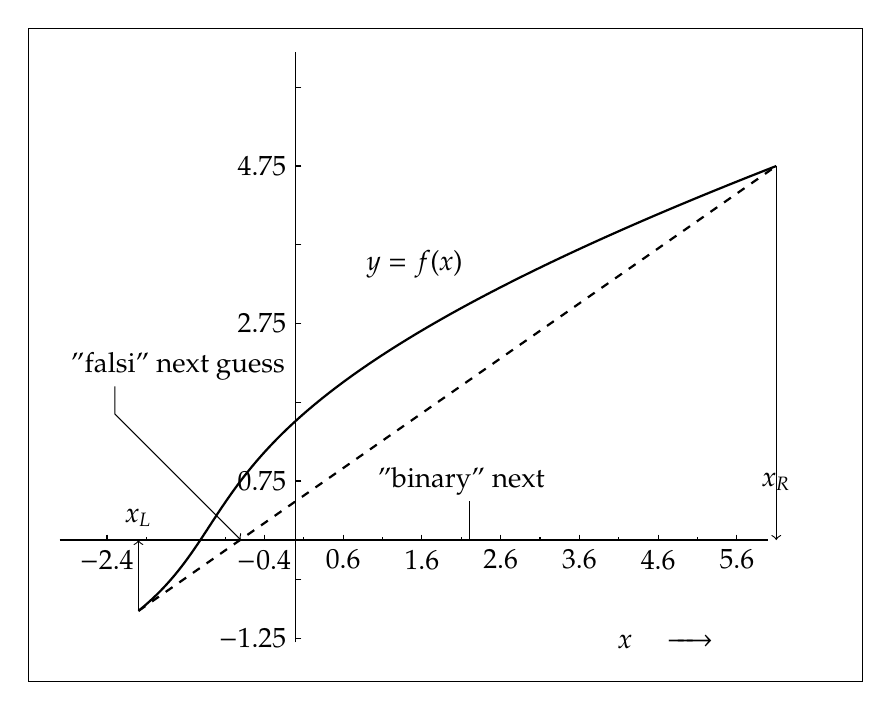
\begin{tikzpicture}
        \draw (-3.4, -1.8) rectangle (7.2,6.5);
        \coordinate (O) at (0,0);
        \draw (-3,0) -- (6,0);
        \draw (0,-1.3) -- (0,6.2);
        \foreach \x in {-2.4,-0.4,0.6,1.6,2.6,3.6,4.6,5.6}
            \draw (\x cm,2pt) -- (\x cm,-0pt) node[anchor=north] {$\x$};
        \foreach \x in {-1.9,...,5.1}
            \draw (\x cm,1pt) -- (\x cm,-0pt);
        \foreach \y in {-1.25,-0.5,0.75,1.75,2.75,3.75,4.75,5.75}
            \draw (2pt,\y cm) -- (0pt,\y cm);
        \foreach \y in {-1.25,0.75,2.75,4.75}
            \node[anchor=east] at (0pt,\y cm) {$\y$};

        \draw (2.2,0) -- ++(0,0.5);
        \node  at (2.1,0.75) {"binary" next};

        %\path[name path=x] (0.3,0.5) -- (6.7,4.7);
        %\path[name path=y] plot[smooth] coordinates {(-0.3,2) (2,1.5) (4,2.8) (6,5)};
        \coordinate (A) at (-2.0, -0.9);
        \coordinate (AB) at (-0.4,+0.4);
        \coordinate (BB) at (-1.6,1.75);
        \coordinate (B) at (-1.4,0);
        \coordinate (C) at (0, 1.75);
        \coordinate (F) at (6.1, 4.75);
        \draw[thick] (A) .. controls (AB) and (BB) .. (F); 
        \node at (1.5,3.5) {$y=f(x)$};
        \draw [thick,dashed] (A) -- (F);
        \coordinate (yaxis) at (0,6);
        \coordinate (xaxis) at (6,0);
        \draw [->] (F) -| (xaxis -| F) node[above, yshift=0.5cm] {$x_R$};
        \draw [->] (A) -| (xaxis -| A) node[above, yshift=0.05cm] {$x_L$};
        \node at (-1.5, 2.2) (fa) {"falsi" next guess};
        \draw [->] ($(fa)+(-0.8,-0.25)$) -- ++(0,-.35cm) -- (-0.7,0);
        \node at (4.7, -1.25) (xarr) {$x\quad \xrightarrow{\hspace*{0.4cm}}$};
        % debug and helpers
        \iffalse
        \draw [blue, very thick] (A) circle (0.1);
        \draw [green, very thick] (BB) circle (0.1) node[anchor=north] {BB};
        \draw [green, very thick] (AB) circle (0.1) node[anchor=north] {AB};
        \draw [blue, very thick] (B) circle (0.1);
        \draw [blue, very thick] (C) circle (0.1);
        \draw [blue, very thick] (F) circle (0.1);
        \draw [red](-0.8,0) -- ++(0,0.5);
        \draw [xshift= 0.1cm, step=0.25,blue, very thick, opacity=0.2] (-2.5,-1.5) grid (6.5,6.5);
        \fi
    \end{tikzpicture}
    \caption{\textit{Graphical illustration of regula falsi}}
    \label{fig:06_04}
\end{figure}

A straight line in the $x-y$ plane has the analytic form
\begin{equation}
    y = ax + b
    \label{eq:06_11}
\end{equation}
where a and b are constants. The intercept of the straight line with the x-axis is gotten by setting y = 0 and solving for x:

\begin{equation}
x\,' = \frac{-b}{a}
\end{equation}

To determine a and b we use the two equations

\begin{equation}
\begin{aligned}
f_L = ax_L + b\\
f_R = ax_R + b
\end{aligned}
\end{equation}

giving

\begin{equation}
    a = \frac{1}{2}\left [f_L + f_R - \frac{f_R - f_L}{x_R - x_L} \big (x_L + x_R \big )\right ]
\end{equation}

and thus

\begin{equation}
x' = \frac{f_Rx_L - f_Lx_R}{f_R - f_L}
\end{equation}

A FORTH flow diagram for this algorithm appears in Fig.\ref{fig:06_05}
%  Fig. 6-5 
\begin{figure}
    \begin{tikzpicture}[minimum size=0.5cm]
        \draw (-2.8, 0.20) rectangle (8,-8.8);
        \node (start) {};
        \node [circle, draw, cross, below= of start] (cross) {};
        \node [below=0.8 of cross] (cond) {};
        \node [below=0.8cm of cond] (cond2) {};
        \node [draw, below right=0.2cm of cond2, text width=1.5cm, align=center] (NO) {NO\\ $\mathrm{x_R=x'}$\\ $\mathrm{f_R=f}$\\ };
        \node [draw, below left=0.2cm of cond2, text width=1.5cm, align=center] (YES) {YES\\ $\mathrm{x_L=x'}$\\ $\mathrm{f_L=f}$\\ };
        \node [draw, below=2.5cm  of cond2] (equ1)  {$\mathrm{x_{old}=x'}$};
        \node [circle, draw, dot, below=0.5cm  of equ1] (dot1)  {};
        \node [below left=0.5cm of cond, minimum height= 0.25cm, xshift=-0.4cm, fill=gray!20]  (ext) {\textbf{DONE}};
        \draw  (start.mid) -- (cross);
        \draw  (cross) -- (cond.mid);
        \draw [->] (cond.mid) -| (ext);
        \draw  (cond.mid) -| (cond2.mid);
        \draw [->] (cond2.mid) -| (YES);
        \draw [->] (cond2.mid) -| (NO);
        \draw [->] (YES.south) -- ++(0,-0.5cm);
        \draw [->] (YES.south) |- ++(0,-0.5cm) -| (equ1);
        \draw [->] (NO.south) -- ++(0,-0.5cm);
        \draw [->] (NO.south)  |- ++(0,-0.5cm) -| (equ1);
        \draw [->] (equ1) -- (dot1);
        \node [right=of cross, xshift= 1.5cm] (cyc) {BEGIN calculate $x'$} ;
        \node [above =0.9cm of cyc.west,anchor=west, align=left, text width=6.5cm] {
            INITIALIZE\\
            $\mathrm{f_L=f(x_L) \quad f_R=f(x_R)}$\\
            $\mathrm{x_{old}=x_L}$};
        \node [below=0.6 of cyc.west, anchor=west, align=left, xshift= 0.5cm] (body) {$\mathrm{\left | {x}' - x_{old} \right |} > error$};
        \node [below=0.1cm of body, anchor=west, align=left, xshift=-2.0cm] {?};
        \node [below=1.4cm of cyc.west, anchor=west, align=left] (while) {WHILE};
        \node [below=0.5cm of while.west, anchor=west, align=left] (eq2) {$\widehat{f}=f({x}')$};
        \node [below=0.5cm of eq2.west, anchor=west, align=left] (eq3) {$sign(\widehat{f}\;) = sign(f_L)$ ?};
        \node [below=0.8cm of eq3.west, anchor=west, align=left, xshift= -0.2cm, yshift=0.25cm] (eq4) { IF   \hspace{1.2cm} $\mathrm{x_L=x \quad f_L=f}$};
        \node [below=0.8cm of eq4.west, anchor=west, align=left] (eq5) { ELSE \hspace{0.5cm} $\mathrm{x_R=x \quad f_R=f}$};
        \node [below=0.8cm of eq5.west, anchor=west, align=left] (eq6) { THEN };
        \node [right=2.0cm of dot1] (eq7) { REPEAT };

    \end{tikzpicture}
    \caption{\textit{Regula falsi algorithm for roots of f(x)}}
    \label{fig:06_05}
\end{figure}


The corresponding program is shown on page 132.

Here is an example of the program in action:

\begin{lstlisting}
    FINIT 6 #PLACE ! ok \ set display to 6 digits
    \ Example: f(x) = exp(-x) - x
    : FNA FDUP FNEGATE FEXP FR- ;
    \ Cleariy, the root lies between 0 and 3. (Why?)

    USE( FNA % 0. % .3 % 1.E-6 )FALSI
    \ st(4) st(3) st(2)  x'      x'-xold
    ?????? ?????? ?????? .759452 -.291530
    ?????? ?????? ?????? .588025 -.0326025
    ?????? ?????? ?????? .569459 -.00362847
    ?????? ?????? ?????? .567400 -.000403560
    ?????? ?????? ?????? .567171 -.0000448740
    ?????? ?????? ?????? .567146 -.0000050002
    ?????? ?????? ?????? .567143 -.0000005544 ok
\end{lstlisting}

The display was generated by the word \textbf{.FS} --placed in the definition of \bc{APART?} for debugging -- we show the top 5 of the eight 80x87 registers. The ?????? means the contents of that register are not a properly defined fp number, either because of a mistake or because nothing was stored in them after \bc{FINIT}. Here, since the program is obviously working, the latter explanation is the correct one.

\section{Ordinary differential equations}
\TallC{We} wish to solve the first-order general differential equation

\begin{equation}
    \dot{x} \equiv \frac{dx}{dt} = f(x,t)
    \label{eq:06_16} 
\end{equation}

In general we can only solve Eq.\ref{eq:06_16} approximately, starting from the value of x -- call it $x_0$ -- at some initial time $t_0$, then advancing the time by small increments $dt = h$, using the differential equation itself to give us $x(t+h)$ given $x(t)$.

For example, we could expand in Taylor's series\sepfootnote{06_11}

\begin{equation}
    x(t+h) = x(t) + h\dot{x}(t) + \frac{h^2}{2}\ddot{x}(t) + ...
    \label{eq:06_17} 
\end{equation}

\begin{lstlisting}
    \ USE( Fname % a % b % err )FALSI
    ( 87:--root )
    \ Fname is the name of a FORTH function

    \ function notation
    : USE( [COMPILE] ' CFA LITERAL ;
           IMMEDIATE

    6 REAL*4 SCALARS ERR XL XR YL YR OLDX

    0 VAR f1 \ a place to store cfa
    : SAME.SIGN? (87:xy -- -- f)
        F* F0> ;

    :INITIALIZE ( cfa -- 87: a b e -- )
        IS f1   \ store cfa
        XDUP    \ interval has root?
        SAME.SIGN?
        ABORT" Even number of roots!!!"
        XR G! XL G!
        XL G@ f1 EXECUTE YL G!
        XR G@ f1 EXECUTE YR G!
        F=0 OLDX G! ;

    : X' XL G@ FR G@ ( 87: -- x')
        FUNDER F*    ( 87: -- yR xL*yR)
        XR G@ YL G@
        FUNDER F* ( 87: -- yR xL*yR xL xR*yL )
        FROT   F- ( 87: -- yR yL xR*yL-xL*yR)
        F-ROT  F- F/ ;

    : APART? ( 87: x' -- x' -- f )
        FDUP OLDX G@ F-
        .FS FABS ERR G@ F> ;

    : REVISE ( 87: x' -- )
        FDUP f1 EXECUTE ( 87: -- x' y')
        FDUP YL G@
        SAME.SIGN? FOVER
        ( --f 87: -- x'y' x')
        IF      XL G! YL G!
        ELSE    XR G! YR G! THEN
        OLDX G! ; ( -- 87: -- )

    : )FALSI ( cfa-- 87: a b e -- root ) INITIALIZE
\end{lstlisting}

and keep only the lowest order terms:

\begin{equation}
x(t+h) \approx x(t) + hf(x(t), t).
    \label{eq:06_18} 
\end{equation}

\subsection{Runge-Kutta method}

One standard class of methods that had fallen into disfavor by now are popular again, are the Runge-Kutta algorithms\sepfootnote{06_12}. The algorithms can be classified according to order n (that is, if $h$ the step size, the error at each step will be $O(h^n)$. The second order Runge-Kutta algorithm is $(x' \equiv x(t+h) , x \equiv x(t) )$

\begin{equation}
\begin{aligned}
    k &= hf(x,t) \\
    x' &= x + \frac{1}{2}\big(k + hf(x+k, t+h)\big) + O(h^3).
    \label{eq:06_19} 
\end{aligned}
\end{equation}

How does this work? Clearly,

\begin{equation}
\begin{aligned}
    k + hf(x+k,t+h) & \approx hf(x,t) + hf(x,t) + h^2\frac{\partial f}{\partial t} + hk \frac{\partial f}{\partial x} \\
    & \equiv 2h\dot{x}(t) + h^2\ddot{x}(t) + O(h^3)
    \label{eq:06_20} 
\end{aligned}
\end{equation}

Substituting \ref{eq:06_19} in \ref{eq:06_20} we now find

\begin{equation*}
    x' = x(t+h) = x(t) + h\dot(t) + \frac{h^2}{2}\ddot{x}(t) ;
\end{equation*}
that is, the Runge-Kutta $x'$ agrees with the Taylor's series expansion \ref{eq:06_17}, to $O(h^3)$.

The flow chart of second-order Runge-Kutta is shown in Fig. \ref{fig:06_06} below. We express the algorithm in FORTH as shown in Fig. \ref{fig:06_07} on page \pageref{fig:06_07} below.

% Fig. 6-6 
\begin{figure}
    \center
    \begin{tikzpicture}[minimum size=0.5cm]
        \draw (-3.0, 0.5) rectangle (6.5,-4.0);
        \node (start) {};
        \node [circle, cross, draw, below=0.6cm of start] (crc) {};
        \node [circle, draw, dot, below=1.5cm of crc] (dot1)  {};
        \draw [->] (start.mid) -- (crc);
        \draw [->] (crc) -- (dot1);
        \node [right=of start.west] (txtstart) {)RUNGE} ;
        \node [below=0.4cm of txtstart.west, anchor=west, xshift= 0.5cm] (cyc) {INITIALIZE:\space get h, tf, t0, x0} ;
        \node [right= of crc.west, anchor=west, align=left] (while) {BEGIN DISPLAY};
        \node [below=0.40cm of while.west, anchor=west, align=left, xshift=0.25cm] (bdy) {DONE? NOT};
        \node [below=0.8cm of while.west, anchor=west, align=left] (w2) {WHILE};
        \node [below=1.2cm of while.west, anchor=west, align=left, xshift=0.25cm] (eq3) {STEP};
        \node [below=1.6cm of while.west, anchor=west, align=left] (rpt) { REPEAT };
    \end{tikzpicture}
    \caption{\textit{2nd-order Runge-Kutta for dx/dt = f(x,t)}}
    \label{fig:06_06}
\end{figure}

% Fig. 6-7.
\begin{figure}
    \tiny
    \begin{tcolorbox} [sidebyside, colback=white, sharp corners, enhanced, segmentation style=solid]
    % first column
    \begin{lstlisting}
\ STRAIGHT 2ND ORDER RUNGE-KUTTA
\ SOLUTION OF FIRST-ORDER DIFEQ
\ dx/dt = f(x,t)

\ See Abramowitz & Stegun, HMF 25.5.6

\ Usege:
\ USE( FNB % x0 % t0 % tf % h )RUNGE
\
\ FNB (:[t]-- 87:x--f[x,t]) evaluates f(x.t)
\ x0 = starting value of dep. variable
\ t0 = initial time
\ tf = end time
\ h = step.size
\
\ k = hf(x,t), x' = x + (k +hf(x+k,t+h))/2

6 REAL*4 SCALARS T T' H X TMAX K
0 VAR f1 \ to hold cfa
: USE( [COMPILE]' CFA LITERAL;
       IMMEDIATE
: INITIALIZE (:cfa-- 87: x0 t0 tf h -- )
    IS f1 H G! TMAX G! T G! X G! ;
    \end{lstlisting}
\tcblower
    %second column
    \begin{lstlisting}
\ These words increment x & t.
: inc.T     T G@ H G@ F+ T' G! ;
: inc.X     X G@
     T  f1 EXECUTE (87:--f[x,t])
     H  G@ F*      (87:--k=hf[x,t])
     FDUP K G!    \ save k
     X  G@ F+      (87:-- x+k)
     T' G@ T G!
     T  f1 EXECUTE (87:--f[x+k,t+h])
     H  G@ F*
     K  G@ F+ F2/
                   (87:--[k+i[x+k,t+h] ]/2)
     X  G@ F+ X G! ;

: DONE? TG@ TMAXG@ F>) ; (:--f)

0 VAR exact            \ cfa
: DISPLAY   exact EXECUTE
    XG@  T  G@ CR F. F. F. ;
\ emit "t x exact"

: )RUNGE      (:cfa-- 87: x0 t0 tf h -- )
        BEGIN DISPLAY
                DONE? NOT
    \end{lstlisting}
    \end{tcolorbox}
    \caption{\textit{Explicit 2nd-order Runge-Kutta solver}}
    \label{fig:06_07}
\end{figure}

As an example of second-order Runge-Kutta in action, let us solve numerically the equation ,

\begin{equation}
    \dot{x} = t^2 e^{-x}
    \label{eq:06_21} 
\end{equation}

with the initial condition x(t = 0) = 0 , whose exact solution is

\begin{equation}
    x(t) =log_e(1 +\frac{1}{3}t^3).
    \label{eq:06_22} 
\end{equation}

% Fig. 6-8 
\begin{figure}
    \centering
    \begin{tabular}{l|l}
        \begin{tabular}{ccc}
            \multicolumn{1}{c}{t} &  \multicolumn{1}{c}{x}  & \multicolumn{1}{c}{$x_{ex}$}\\
                .0000  & .0000  & .0000   \\
                .10000 & .00050 & .00033  \\
                .20000 & .00300 & .00266  \\
                .30000 & .00946 & .00896  \\
                .40000 & .02177 & .02111  \\
                .50000 & .04164 & .04082  \\
                .60000 & .07049 & .06953  \\
                .70000 & .10934 & .10825  \\
                .80000 & .15875 & .15757  \\
                .90000 & .21877 & .21752  \\
                1.0000 & .28896 & .28768  \\
                1.1000 & .36846 & .36718  \\
                1.2000 & .45612 & .45489  \\
                1.3000 & .55063 & .54946  \\
                1.4000 & .65061 & .64954  \\
                1.5000 & .75473 & .75377  \\
                1.6000 & .86175 & .86091  \\
                1.7000 & .97061 & .96989  \\
                1.8000 & 1.0803 & 1.0797  \\
                1.9000 & 1.1902 & 1.1897  \\
                2.0000 & 1.2996 & 1.2992  \\
                2.1000 & 1.4080 & 1.4078  \\
                2.2000 & 1.5151 & 1.5149  \\
                2.2999 & 1.6206 & 1.6205  \\
                2.3999 & 1.7242 & 1.7241  \\
                2.4999 & 1.8258 & 1.8258  \\
            \end{tabular}
&
        \begin{tabular}{ccc}
            \multicolumn{1}{c}{t} &  \multicolumn{1}{c}{x}  & \multicolumn{1}{c}{$x_{ex}$}\\
            2.5999 & 1.9254 & 1.9255 \\ 
            2.6999 & 2.0228 & 2.0230 \\ 
            2.7999 & 2.1181 & 2.1183 \\ 
            2.8999 & 2.2113 & 2.2115 \\ 
            2.9999 & 2.3023 & 2.3025 \\ 
            3.0999 & 2.3912 & 2.3915 \\ 
            3.1999 & 2.4781 & 2.4784 \\ 
            3.2999 & 2.5630 & 2.5633 \\ 
            3.3999 & 2.6459 & 2.6462 \\ 
            3.4999 & 2.7270 & 2.7273 \\ 
            3.5999 & 2.8061 & 2.8065 \\ 
            3.6999 & 2.8836 & 2.8839 \\ 
            3.7999 & 2.9592 & 2.9596 \\ 
            3.8999 & 3.0333 & 3.0336 \\ 
            3.9999 & 3.1057 & 3.1060 \\ 
            4.0999 & 3.1766 & 3.1769 \\ 
            4.1999 & 3.2460 & 3.2463 \\ 
            4.2999 & 3.3139 & 3.3142 \\ 
            4.3999 & 3.3804 & 3.3808 \\ 
            4.4999 & 3.4456 & 3.4460 \\ 
            4.5999 & 3.5095 & 3.5099 \\ 
            4.6999 & 3.5722 & 3.5725 \\ 
            4.7999 & 3.6336 & 3.6339 \\ 
            4.8999 & 3.6939 & 3.6942 \\ 
            4.9999 & 3.7531 & 3.7534 \\ 
            5.0999 & 3.8111 & 3.8114 \\ 
        \end{tabular}
        \\
\end{tabular}
    \caption{\textit{Second order Runge-Kutta -- results}}
    \label{fig:06_08}
\end{figure}

Thus define

\begin{lstlisting}
    : FNB (:[T]-- 87: x--f[x,t])
        FNEGATE FEXP G@ F**2 F*
    : EXACT T G@ FDUP FDUP F* F* (87:--t^3)
        3 S->F F/ F=1 F+ FLN ;
\end{lstlisting}

and say

\begin{lstlisting}
    USE( EXACT IS exact ok
    USE( FNB % 0. % 0. % 5. % 0.1 )RUNGE
\end{lstlisting}

The resulting output is shown in Fig. \ref{fig:06_08} above.

\subsection{An implicit Runge-Kutta formula}
\TallC{A variation} on straight Runge-Kutta is a so-called \textbf{implicit} algorithm\sepfootnote{06_13}.For example, in the second-order formulae given above, suppose $x + k$ were replaced by $x'$:

\begin{equation}
\begin{aligned}
    k &= hf(x,t)\\
    x' &= x + \frac{1}{2}\big(k + hf(x',t+h)\big) + O(h^3)
    \label{eq:06_23} 
\end{aligned}
\end{equation}

and the resulting (transcendental) equation solved for x' by --say-- \textit{regula falsi}. Since we have already written a \textit{regula falsi} program, we can apply it here to get the algorithm shown diagrammatically in Fig. \ref{fig:06_09} below. We program it\sepfootnote{06_14} as shown in Fig. \ref{fig:06_10} on page \pageref{fig:06_10} below.

% Fig. 6-9 
\begin{figure}
    \begin{tikzpicture}[minimum size=0.5cm]
        \draw (-1.5, 0.5) rectangle (9,-4.0);
        \node (start) {};
        \node [circle, draw, below= of start] (crc) {};
        \node [circle, draw, dot, below=1.5cm of crc] (dot1)  {};
        \draw [->] (start.mid) -- (crc);
        \draw [->] (crc) -- (dot1);
        \node [right=of start.west] (txtstart) {)RUNGE} ;
        \node [below=0.25cm of txtstart, anchor=west, xshift=-0.5cm] (cyc) {INITIALIZE:\space get h, tf, t0, x0} ;
        \node [right= of crc.west, anchor=west, align=left] (while) {BEGIN DISPLAY};
        \node [below=0.40cm of while.west, anchor=west, align=left, xshift=0.25cm] (bdy) {DONE? NOT};
        \node [below=0.8cm of while.west, anchor=west, align=left] (w2) {WHILE};
        \node [below=1.2cm of while.west, anchor=west, align=left, xshift=0.25cm] (eq3) {k=hf(x,t)};
        \node [below=0.40cm of eq3.west, anchor=west, align=left, xshift=0.15cm] (eq4) {SOLVE: \space x' = x + k/2 + hf(x',t+h)/2};
        \node [right= of dot1.west, anchor=west, align=left] (rpt) { REPEAT };
    \end{tikzpicture}
    \caption{\textit{2nd-order \underline{implicit} Runge-Kutta for dx/dt = f(x,t)}}
    \label{fig:06_09}
\end{figure}

Now we consider the same example as previously:

\begin{lstlisting}
    : FNB (:[T]-- 87:x--f[x,t])
        FNEGATE FEXP G@ F**2 F' ;
    : EXACT T G@ FDUP FDUP F* F* (87: -- t^3)
        F=3 F/ F=1 F+ FLN ;
\end{lstlisting}

and say
\begin{lstlisting}
    USE( EXACT IS exact ok
    USE( FNB % 0. % 0. % 5. % 0.1 )RUNGE ok
\end{lstlisting}

% Fig. 6-10.
\begin{figure}
    \tiny
    \begin{tcolorbox} [sidebyside, colback=white, sharp corners, enhanced, segmentation style=solid]
    % first column
    \begin{lstlisting}
FIND )FALSI 0= ?( FLOAD FALSI.FTH )
7REAL*4 SCALARS T T' H X X' TMAX K
0 VAR f1    \ to hold cfa of f(xt)
: INITIALIZE IS f1
        H G! TMAX G! T G! X G! ;

\ These words Increment x & t.
: inc.T T G@ H G@ F+ T' G! ;
: k     X G@
    T f1 EXECUTE   ( 87:--f[x,t])
    H G@ F* K G! ; ( 87:--k=hf(x,t)

: X" ( 87:x'--g[x'])
    T f1 EXECUTE   ( 87:--f[x',t+h])
    H G@ F* K G@ F+ F2/
     ( 87:--[k+f[x+k,t+h] ]/2)
    \end{lstlisting}
\tcblower
    %second column
    \begin{lstlisting}
    X G@ F+ ;
% 3. FCONSTANT F=3
: INTERVAL X G@ FDUP
       K G@ F=3 F* F+ ;

: X' USE( X" INTERVAL % 1.E-6
       )FALSI ;
: inc.X k X' X G! T' G@ T G! ;
: DONE? T G@ TMAX G@ F> ;
      (:--f)
0 VAR exact         \ cfa
: DISPLAY    exact EXECUTE
    X G@ T G@ CR F. F. F. ;
\ emit "t x exact"
: )RUNGE (:cfa--87:x0 t0 tf h -- )
    BEGIN DISPLAY
    \end{lstlisting}
    \end{tcolorbox}
    \caption{\textit{Implicit 2nd-order Runge-Kutta program}}
    \label{fig:06_10}
\end{figure}

The resulting output is shown in Fig. \ref{fig:06_11} on page \pageref{fig:06_11}.

Clearly the implicit form is more accurate; whether the putative gain in stability justifies solving a transcendental equation is unclear, however.

% Fig. 6-11 
\begin{figure}
    %\tiny
    \centering
    \begin{tabular}{l|l}
        \begin{tabular}{ccc}
            \multicolumn{1}{c}{t} & 
            \multicolumn{1}{c}{x} & 
            \multicolumn{1}{c}{$x_{ex}$}\\
            .00000 & .00000 & .00000 \\
            .10000 & .00050 & .00033 \\
            .20000 & .00299 & .00266 \\
            .30000 & .00945 & .00896 \\
            .40000 & .02173 & .02111 \\
            .50000 & .04155 & .04082 \\
            .60000 & .07032 & .06953 \\
            .70000 & .10906 & .10825 \\
            .80000 & .15834 & .15757 \\
            .90000 & .21822 & .21752 \\
            1.0000 & .28825 & .28768 \\
            1.1000 & .36762 & .36718 \\
            1.2000 & .45518 & .45489 \\
            1.3000 & .54962 & .54946 \\
            1.4000 & .64958 & .64954 \\
            1.5000 & .75370 & .75377 \\
            1.6000 & .86077 & .86091 \\
            1.7000 & .96969 & .96989 \\
            1.8000 & 1.0795 & 1.0797 \\
            1.9000 & 1.1895 & 1.1897 \\
            2.0000 & 1.2990 & 1.2992 \\
            2.1000 & 1.4075 & 1.4078 \\
            2.2000 & 1.5147 & 1.5149 \\
            2.2999 & 1.6202 & 1.6205 \\
            2.3999 & 1.7239 & 1.7241 \\
            2.4999 & 1.8256 & 1.8258 \\
        \end{tabular}
        &
        \begin{tabular}{ccc}
            \multicolumn{1}{c}{t} &  \multicolumn{1}{c}{x}  & \multicolumn{1}{c}{$x_{ex}$}\\
            2.5999 & 1.9253 & 1.9255 \\
            2.6999 & 2.0228 & 2.0230 \\
            2.7999 & 2.1181 & 2.1183 \\
            2.8999 & 2.2113 & 2.2115 \\
            2.9999 & 2.3024 & 2.3025 \\
            3.0999 & 2.3914 & 2.3915 \\
            3.1999 & 2.4783 & 2.4784 \\
            3.2999 & 2.5632 & 2.5633 \\
            3.3999 & 2.6461 & 2.6462 \\
            3.4999 & 2.7272 & 2.7273 \\
            3.5999 & 2.8064 & 2.8065 \\
            3.6999 & 2.8838 & 2.8839 \\
            3.7999 & 2.9595 & 2.9596 \\
            3.8999 & 3.0336 & 3.0336 \\
            3.9999 & 3.1060 & 3.1060 \\
            4.0999 & 3.1769 & 3.1769 \\
            4.1999 & 3.2463 & 3.2463 \\
            4.2999 & 3.3142 & 3.3142 \\
            4.3999 & 3.3808 & 3.3808 \\
            4.4999 & 3.4460 & 3.4460 \\
            4.5999 & 3.5099 & 3.5099 \\
            4.6999 & 3.5725 & 3.5725 \\
            4.7999 & 3.6340 & 3.6339 \\
            4.8999 & 3.6942 & 3.6942 \\
            4.9999 & 3.7534 & 3.7534 \\
            5.0999 & 3.8114 & 3.8114 \\
        \end{tabular}
        \\
    \end{tabular}
    \caption{\textit{Second order \underline{implicit} Runge-Kutta -- results}}
    \label{fig:06_11}
\end{figure}

Let us now compare the two algorithms for functions f(x,t) that lead to singular solutions. This time we consider the equation

\begin{equation}
\dot{x} = t^2e^x
\end{equation}

whose exact solution is

\begin{equation}
x(t) = -log_e(1-\frac{1}{3}t^3).
\label{eq:06_25}
\end{equation}

Manifestly, \ref{eq:06_25} blows up at $t = 3^\frac{1}{3}=1.442...$ We expect the behavior to become apparent in the numerical solution. So we say

\begin{lstlisting}
    : FNB FEXP G@ F**2 F* ;
        ([t] -- 87: x -- f[x,t])

    : EXACT F=1 T G@    (87:--t^3)
        FDUP FDUP F* F* F=3 F/ F+ FLN ;
\end{lstlisting}

and say again
\begin{lstlisting}
    USE( EXACT IS exact ok
    USE( FNB % 0. %0 % 5. % 0.1 )RUNGE ok
\end{lstlisting}

The results of doing this with straight-, and then implicit Runge-Kutta are displayed in Fig. \ref{fig:06_12} (p. \pageref{fig:06_12}) and \ref{fig:06_13} (p. \pageref{fig:06_13}), respectively. We only show the second half of the interval (near the singular point) in either case.

The straight Runge-Kutta algorithm, without the fancy implicit solution for $x(t +h)$, appears more accurate near the singularity, although both methods are acceptably accurate. Does this mean implicit Runge-Kutta is no good? No!

The implicit scheme lost accuracy through roundoff: the arithmetic was insufficiently precise. To take advantage of the method's power, we must increase the precision beyond one part in $10^{6}$. This requires changing all scalars to 64-bit precision (\regc{REAL*8}) rather than 32-bit as we have done here. The generic fetch/store techniques developed in Chapter 5 and used here, permit this change with a minimum of fuss. We leave this as an exercise.

% Fig. 6-12 
\begin{figure}
    %\tiny
    \centering
    \begin{tabular}{l|l}
        \begin{tabular}{ccc}
            \multicolumn{1}{c}{t} &  \multicolumn{1}{c}{x}  & \multicolumn{1}{c}{$x_{ex}$}\\
            .71999 & .13287 & .13286 \\  
            .72999 & .13889 & .13888 \\  
            .73999 & .14512 & .14511 \\  
            .74999 & .15156 & .15154 \\  
            .75999 & .15821 & .15820 \\  
            .76999 & .16509 & .16508 \\  
            .77999 & .17220 & .17219 \\  
            .78999 & .17955 & .17954 \\  
            .79999 & .18714 & .18713 \\  
            .80999 & .19499 & .19497 \\  
            .81999 & .20309 & .20308 \\  
            .82999 & .21147 & .21145 \\  
            .83999 & .22012 & .22010 \\  
            .84999 & .22906 & .22904 \\  
            .85999 & .23829 & .23828 \\  
            .86939 & .24783 & .24782 \\  
            .87999 & .25769 & .25767 \\  
            .88999 & .26788 & .26786 \\  
            .89999 & .27841 & .27839 \\  
            .90999 & .28928 & .28926 \\  
            .91999 & .30053 & .30051 \\  
            .92999 & .31215 & .31213 \\  
            .93999 & .32417 & .32415 \\  
            .94999 & .33660 & .33657 \\  
            .95999 & .34945 & .34943 \\  
            .96999 & .36274 & .36272 \\  
            .97999 & .37650 & .37648 \\  
            .98999 & .39074 & .39072 \\  
            .99999 & .40548 & .40546 \\  
            1.0099 & .42075 & .42073 \\  
            1.0199 & .43656 & .43654 \\  
            1.0299 & .45295 & .45293 \\  
            1.0399 & .46995 & .46993 \\  
            1.0499 & .48757 & .48755 \\  
            1.0599 & .50586 & .50584 \\  
            1.0699 & .52485 & .52483 \\  
            1.0799 & .54458 & .54456 \\ 
        \end{tabular}
        &
        \begin{tabular}{ccc}
            \multicolumn{1}{c}{t} &  \multicolumn{1}{c}{x}  & \multicolumn{1}{c}{$x_{ex}$}\\
            1.0899 & .56508 & .56506 \\
            1.0999 & .58640 & .58638 \\
            1.1099 & .60860 & .60857 \\
            1.1199 & .63171 & .63169 \\
            1.1299 & .65580 & .65578 \\
            1.1399 & .68093 & .68091 \\
            1.1499 & .70718 & .70715 \\
            1.1599 & .73461 & .73458 \\
            1.1699 & .76331 & .76329 \\
            1.1799 & .79337 & .79335 \\
            1.1899 & .82491 & .82489 \\
            1.1999 & .85803 & .85801 \\
            1.2099 & .89287 & .89286 \\
            1.2199 & .92959 & .92958 \\
            1.2299 & .96834 & .96834 \\
            1.2399 & 1.0093 & 1.0093 \\
            1.2499 & 1.0527 & 1.0527 \\
            1.2599 & 1.0989 & 1.0989 \\
            1.2699 & 1.1481 & 1.1482 \\
            1.2799 & 1.2007 & 1.2008 \\
            1.2899 & 1.2571 & 1.2572 \\
            1.2999 & 1.3179 & 1.3180 \\
            1.3099 & 1.3836 & 1.3837 \\
            1.3199 & 1.4550 & 1.4552 \\
            1.3299 & 1.5332 & 1.5334 \\
            1.3399 & 1.6193 & 1.6196 \\
            1.3499 & 1.7151 & 1.7154 \\
            1.3599 & 1.8226 & 1.8231 \\
            1.3699 & 1.9449 & 1.9457 \\
            1.3799 & 2.0865 & 2.0876 \\
            1.3899 & 2.2539 & 2.2557 \\
            1.3999 & 2.4581 & 2.4611 \\
            1.4099 & 2.7187 & 2.7242 \\
            1.4199 & 3.0760 & 3.0884 \\
            1.4299 & 3.6376 & 3.6782 \\
            1.4399 & 4.8831 & 5.3657 \\
            & & \\
        \end{tabular}
        \\
    \end{tabular}
    \caption{\textit{Straight Runge-Kulta for singular case}}
    \label{fig:06_12}
\end{figure}

% Fig. 6-13 
\begin{figure}
    %\tiny
    \centering
    \begin{tabular}{l|l}
        \begin{tabular}{ccc}
            t &  x  & $x_{ex}$ \\
            .71999 & .13288 & .13286 \\
            .72999 & .13890 & .13888 \\
            .73999 & .14513 & .14511 \\
            .74999 & .15156 & .15154 \\
            .75999 & .15822 & .15820 \\
            .76999 & .16510 & .16508 \\
            .77999 & .17221 & .17219 \\
            .78999 & .17956 & .17954 \\
            .79999 & .18715 & .18713 \\
            .80999 & .19500 & .19497 \\
            .81999 & .20310 & .20308 \\
            .82999 & .21148 & .21145 \\
            .83999 & .22013 & .22010 \\
            .84999 & .22907 & .22904 \\
            .85999 & .23831 & .23828 \\
            .86999 & .24785 & .24782 \\
            .87999 & .25771 & .25767 \\
            .88999 & .26789 & .26786 \\
            .89999 & .27842 & .27839 \\
            .90999 & .28930 & .28926 \\
            .91999 & .30055 & .30051 \\
            .92999 & .31217 & .31213 \\
            .93999 & .32419 & .32415 \\
            .94999 & .33662 & .33657 \\
            .95999 & .34947 & .34943 \\
            .96999 & .36277 & .36272 \\
            .97999 & .37653 & .37648 \\
            .98999 & .39077 & .39072 \\
            .99999 & .40551 & .40546 \\
            1.0099 & .42078 & .42073 \\
            1.0199 & .43660 & .43654 \\
            1.0299 & .45300 & .45293 \\
            1.0399 & .46999 & .46993 \\
            1.0499 & .48762 & .48755 \\
            1.0599 & .50592 & .50584 \\
            1.0699 & .52491 & .52483 \\
        \end{tabular}
        &
        \begin{tabular}{ccc}
            t &  x  & $x_{ex}$ \\
            1.0799 & .54464 & .54456 \\
            1.0899 & .56515 & .56506 \\
            1.0999 & .58648 & .58638 \\
            1.1099 & .60868 & .60857 \\
            1.1199 & .63180 & .63169 \\
            1.1299 & .65590 & .65578 \\
            1.1399 & .68104 & .68091 \\
            1.1409 & .70729 & .70715 \\
            1.1599 & .73473 & .73458 \\
            1.1699 & .76346 & .76329 \\
            1.1799 & .79353 & .79335 \\
            1.1899 & .82508 & .82489 \\
            1.1999 & .85822 & .85801 \\
            1.2099 & .89309 & .89286 \\
            1.2199 & .92983 & .92958 \\
            1.2299 & .96861 & .96834 \\
            1.2399 & 1.0096 & 1.0093 \\
            1.2499 & 1.0531 & 1.0527 \\
            1.2599 & 1.0993 & 1.0989 \\
            1.2699 & 1.1486 & 1.1482 \\
            1.2799 & 1.2013 & 1.2008 \\
            1.2899 & 1.2578 & 1.2572 \\
            1.2999 & 1.3186 & 1.3180 \\
            1.3099 & 1.3845 & 1.3837 \\
            1.3199 & 1.4561 & 1.4552 \\
            1.3299 & 1.5345 & 1.5334 \\
            1.3399 & 1.6209 & 1.6196 \\
            1.3499 & 1.7171 & 1.7154 \\
            1.3599 & 1.8252 & 1.8231 \\
            1.3699 & 1.9485 & 1.9457 \\
            1.3799 & 2.0914 & 2.0876 \\
            1.3899 & 2.2612 & 2.2557 \\
            1.3999 & 2.4698 & 2.4611 \\
            1.4099 & 2.7395 & 2.7242 \\
            1.4199 & 3.1222 & 3.0884 \\
            1.4299 & 3.8149 & 3.6782 \\
        \end{tabular}
        \\
    \end{tabular}
    \caption{\textit{Implicit Runge-Kutta for singular case }}
    \label{fig:06_13}
\end{figure}
        % % Chapter 7 -- Complex arithmetic in FORTH

\chapter{Complex arithmetic in FORTH}

\TallC{One} of the most crucial features of FORTRAN for scientific computation is the ease with which it embeds complex arithmetic into formulae. No other compiled language has this feature\sepfootnote{07_01}. From time to time someone gets a bright idea, and adds complex arithmetic to Pascal \textit{via} subroutines (since Pascal functions can return only a single number, and complex functions must return two numbers)\sepfootnote{07_02} . The same problem would afflict C and the new structured BASICs.

Recently, a mechanism for adding complex arithmetic to Pascal by defining a stack and using postfix notation has been proposed\sepfootnote{07_03}. Does this sound at all familiar?

This chapter deals with complex arithmetic and its implementation in FORTH. We do not consider complex numbers whose real and imaginary parts are integers, since these are virtually useless in scientific computing. Therefore we perform complex arithmetic solely in single- or double-precision floating point format. We begin with a brief review of the complex number system.

\section{The complex number system}
\TallC{The} algebraic equation

\begin{equation}
  x^2 - 1 = 0
\end{equation}

has 2 roots, $\pm1$, in the standard number system (real numbers). But the (otherwise quite similar) equation

\begin{equation}
  x^2 + 1 = 0
\end{equation}

has \textbf{no} roots. That is, there is no ordinary number which, when squared, gives a negative result. Eighteenth century mathematicians misliked a state of affairs wherein some polynomial equations of n'th degree had n roots, whereas others had n-2, n-4, \etc This seemed disorderly and unpredictable. How much simpler life would be if every polynomial of n'th order could \textbf{always} be factored into n primitives of the form ($x_n$ are \textbf{roots})

\begin{equation}
  \begin{aligned}
    a_0 & + a_1x + a_2x^2 + \ldots + a_nx^n \\
    & \equiv a_n(x-x_1)(x-x_2) \ldots (x-x_n)
  \end{aligned}
\end{equation}

\subsection{Cartesian representation of complex numbers}
\TallC{In} order that every polynomial have n roots it was necessary to extend the idea of \textbf{number} to include objects of the form

\begin{equation}
  z = x\ 1 + y\text{ i}
\end{equation}

where $i$ is ---\,by definition\,--- a ``number'' whose square is $-1$; 1 is a ``number'' whose square is $+1$, and $x$ and $y$ are ordinary numbers. Conventionally, $x$ is called the \textbf{real part} of $z$, and $y$ the \textbf{imaginary part}:

\begin{equation}
  x = \text{Re$(z)$ , $y =$ Im$(z)$.}
\end{equation}

Thus the solutions of the polynomial equation

\begin{equation}
  z^2 + 1 = 0
\end{equation}

are

\begin{equation}
  z = 01 \pm 1\text{i}
\end{equation}

(that is, $x = 0, y = \pm1$).

To reassure readers who find uncomfortable the notion of a "number" \textbf{i} $= \sqrt{-1}$ whose square is negative, it is possible to find a $2\times2$ \textbf{matrix representation} for \textbf{1} (unit matrix) and \textbf{i}:

\begin{equation}
  1 =
  \begin{pmatrix}
    1 & 0 \\ 0 & 1
  \end{pmatrix}
  \; , \; i =
  \begin{pmatrix}
    0 & 1 \\ -1 & 0
  \end{pmatrix}
\end{equation}

It is easy to verify that\,---\,in the sense of matrix multiplication\,---

\begin{equation}
  \text{i $\times$ i $= -1$, $1 \times$ i $=$ i $\times 1$, and $1 \times 1 = 1$.}
\end{equation}

These are just the usual multiplication rules for complex numbers. Note that $x$ 1 and $y$ i then mean multiplication of a matrix by a scalar:

\begin{equation*}
  \begin{aligned}
    x\ 1 \equiv
    \begin{pmatrix}
      x & 0 \\ 0 & x
    \end{pmatrix}
    \ ,\ y \text{ i} \equiv
    \begin{pmatrix}
      0 & y \\ -y & 0
    \end{pmatrix}\\
    z = x + iy \equiv
    \begin{pmatrix}
      x & y \\ -y & x
    \end{pmatrix}
  \end{aligned}
\end{equation*}

\TallC{The} complex numbers obey all the algebraic rules of ordinary arithmetic\,---\,commutative and associative laws of multiplication and addition. They are \textbf{complete} in the sense that when we multiply or add two complex numbers we get a \textbf{complex} number, not some other kind of number:

\begin{equation}
  \begin{aligned}
    (a + ib)\ (x + iy) = (ax - by)\ +\ i(ay + bx) \\
    (a + ib)\ (x + iy) = (ax - by)\ +\ i(ay + bx)
  \end{aligned}
\end{equation}

For every complex number, $z = x + iy$ there is a corresponding \textbf{complex conjugate} complex number,

\begin{equation}
  z^* = x - iy.
\end{equation}

Each non-zero complex number $z$ has a \textbf{multiplicative inverse} $1/z\ldots$ To see this, multiply numerator and denominator of $1/z$ by the complex conjugate Eq. 11, and note that

\begin{equation*}
  zz^* \equiv z^*z = x^2 + y^2
\end{equation*}

is a non-zero \textbf{real} number. We can therefore calculate its inverse by ordinary division, and (scalar-) multiply $z^*$ by the result:

\begin{equation}
  \frac{1}{z_2} \equiv \frac{z_2^*}{z_2z_2^*} \equiv \left(\frac{x_2}{x_2^2 + y_2^2} - i \frac{y_2}{x_2^2 + y_2^2}\right).
\end{equation}

To \textbf{divide} one complex number $z_1$ by another, $z_2$, invert $z_2$ and multiply: $z_1/z_2 \equiv z_1 \times (1/z_2)$, \ie

\begin{equation}
  \frac{z_1}{z_2} \equiv \big(x_1 + iy_1\big) \times \left(\frac{x_2}{x{^2}{_2} + y{^2}{_2}} - i \frac{y_2}{x_2^2 + y_2^2}\right)
\end{equation}

(Numbers that satisfy the addition, multiplication and closure properties of real or complex numbers are said to form a \textbf{field}.)

It is easy to prove that even when the coefficients of an n'th degree polynomial are \textbf{complex}, it has n roots that can be represented as complex numbers.

Complex numbers can be used to represent points in the $x$-$y$ plane with $y$ plotted vertically and $x$ horizontally\sepfootnote{07_04}. ( Sometimes this graphical representation is called an \textbf{Argand plot} or \textbf{Argand diagram}. The $x$-$y$ plane is then called the \textbf{Argand plane}.)

\begin{figure}
    \center
    TODO figure 7.1
    \caption{\textit{Representing a complex number as a point in the Argand plane, in Cartesian and polar coordinates}}
    \label{fig:07_01}
\end{figure}

\subsection{Polar representation of complex numbers}

The complex number $z = x + iy$ is said (remember the Argand plane) to be represented in \textbf{Cartesian} form (after Ren\'e Descartes, the inventor of analytic geometry, \ie the idea of graphing equations). However, it is equally valid to use the relationship (\textbf{Euler’s theorem})

\begin{equation}
  e^{i\theta} \equiv \cos \theta + i \sin \theta
\end{equation}

to write the \textbf{polar representation} of $z$,

\begin{equation}
  z = re^{i\theta}\ ,\ r \geq 0.
\end{equation}

Clearly, since $z^* \equiv r\ e^{-i\theta}$, we have

\begin{equation}
  r = \sqrt{zz^*} = \big(x^2 + y^2\big)^\frac{1}{2}
\end{equation}

and\sepfootnote{07_05}

\begin{equation}
  \theta = tan^{-1}(y/x).
\end{equation}

Note that $\theta$, sometimes called Arg($z$), is defined only up to multiples of $2\pi$\,---\,that is, adding $2\pi$ to an angle changes neither \textit{sine} nor \textit{cosine} because of their periodicity. The relations between $(x,y)$ and $(r,\theta)$ are illustrated in Fig. 7-1 above:

\section{Load, store, manipulate fstack}
\TallC{We} now define FORTH words to perform complex arithmetic. All complex operations will be prefixed by the letter X\sepfootnote{07_06}. We assume all complex operations are performed on the FPU for speed, hence we shall give 87stack diagrams.

In 87stack (or fstack) diagrams 2 stands for complex number, x for real part, and y for imaginary part. Where useful, the 87stack diagrams show the operations decomposed into real and imaginary parts. By convention the imaginary part is higher on the fstack than the real part.

By now most FORTH code should be self-explanatory. Many words have been coded in high-level FORTH because the overhead of threading is negligible compared with the time spent executing.

With by-now obvious meanings we have

\begin{lstlisting}
    \ -- single & double-precision complex fetch and store.
    : X@    DUP R32@ 4+ R32@ ; ( adr-- 87:--z )
    : X!    DUP 4+ R32! R32! ; ( adr-- 87:z-- )
    CODE    8+ BX 08 IW ADD. END-CODE
    : DX@   DUP R64@ 8+ R64@ ; ( adr-- 87:--z )
    : DX!   DUP 8+ R64! R64! ; ( adr-- 87:z-- )
    \ -- and complex fetch and store.

    \ fstack manipulation
    :REAL   FDROP ;      ( 87:z--x )
    :IMAG   FPLUCK ;     ( 87:z--y )
    :CONJG  FNEGATE ;    ( 87:xy--x,-y )

    :XDROP FDROP FDROP ; ( 87:z-- )
    :XSWAP F4R F4R ;     ( 87:z1 z2--z2 z1 )
    :XDUP FOVER FOVER ;  ( 87:z--z z )
\end{lstlisting}

\section{Arithmetic operations}
\TallC{The} standard complex operations should be virtually self-explanatory. For efficiency we define multiplication and division of a complex number by a scalar, as well as complex $\times$ complex and complex/complex.

\begin{lstlisting}
    :CMPLX F=0 ;     ( 87: x--x 0 )
    : X+ FROT F+  F-ROT F+ FSWAP ;
    : X- FROT FR- F-ROT F- FSWAP ;
    : XOVER FSP F3P; ( 87:z1 z2--z1 z2 z1 )
    : X*F            ( 87:x y a -- ax ay )
        FUNDER F*    ( 87:--a x bx )
        F-ROT  F* FSWAP ;
    : F*X FROT X*F ; ( 87:x a b--ax bx )
    \ CODE X*F 2FMUL'. 1FMULP. END-CODE
    : X*I FNEGATE FSWAP ;
    : X/F 1/F X*F ;
\end{lstlisting}

The critical operation of complex $\times$ complex can be defined in high level FORTH for portability:

\begin{lstlisting}
  : X*              ( 87:z1 z2--z1*z2 )
    XOVER X*I FROT  ( 87:--a b x -b a y )
    X*F             ( 87:--a b x -by ay )
    F3X FSWAP       ( 87:--a ay x b -by )
    F4X FSWAP       ( 87:-- -by ay x a b )
    F*X             ( 87:-- -by ay xa xb )
    X+ ;
\end{lstlisting}

Actually, complex multiplication is sufficiently involved to be worth defining in code. Here is a code definition for the 80x87 family of FPUs. The equivalent for the Motorola 68881/2 family is virtually identical, allowing for minor differences in Intel and Motorola assembler mnemonics, as well as for the fact that the 68881/2 has registers but no stack.

\begin{lstlisting}
  \ operation     87stack contents
  CODE X*       \ x      y  a  b
    3 FLD.      \ x      y  a  b x
    2 FMUL.     \ x      y  a  b xa
    4 FXCH.     \ xa     y  a  b x
    1 FMUL.     \ xa     y  a  b xb
    1 FXCH.     \ xa     y  a xb  b
    3 FMUL.     \ xa     y  a bx yb
    4 FSUBRP.   \ xa-yb  y  a bx
    2 FXCH.     \ xa-yb bx  a y
    1 FMULP.    \ xa-yb bx ay
    1 FADDP.    \ xa-yb bx+ay
  ENDCODE ( x y a b -- xa-yb xb+ya )
\end{lstlisting}

\TallC{Once} we have multiplication, division is easy:

\begin{lstlisting}
    : XMODSQ            ( 87:x y--x**2+y**2 )
        F**2 FSWAP F**2 F+ ;
    : 1/X CONJG XDUP XMODSQ
        FDUP F0= ABORT" Can't divide by 0" X/F ;
    :X/ 1/X X* ;        ( 87:z1 z2--z1/z2 )
\end{lstlisting}

With the preceding discussion and referring to Fig. 7-1 at page 147 the FORTH words to accomplish Cartesian-polar transformation and \textit{vice versa} should also be fairly transparent\sepfootnote{07_07}:

\begin{lstlisting}
    : ARG FSWAP FPATAN ; ( 87:x y--atan[y/x] )
    SYNONYM FATAN2 ARG
    \ FORTRAN defines FATAN2 so we do also.

    :XABS                ( 87:z--|z| )
        XMODSQ FSQRT ;

    : >POLAR             ( 87:x y--r $\theta$[radians] )
        XDUP XABS F-ROT ARG ;
    :POLAR>              ( 87:r $\theta$[radians]--x y )
        FSINCOS FROT X*F ;
\end{lstlisting}

\section{Roots of complex numbers}
\TallC{The} n'th root of a complex number $z$ is that complex number, $z^{1/n}$, whose n'th power is the original number. That is, as for real numbers,

\begin{equation}
  \left(z^{1/n}\right)^n \equiv z
\end{equation}

It might seem almost trivial to define the n’th root of a complex number in polar representation:

\begin{equation}
  z = r\ e^{i\theta}
\end{equation}

hence

\begin{equation}
  z^{1/n} = r^{1/n} e^{i\theta/n}
  \label{eq:07_20}
\end{equation}

Certainly we know what we mean by the n‘th root of a positive real number, and from Euler’s theorem we know how to evaluate

\begin{equation}
  e^{i\theta/n} \equiv \cos\frac{\theta}{n} + i \sin\frac{\theta}{n}
\end{equation}

However, we can also think of the n'th root as a solution of the polynomial equation in the variable $w$

\begin{equation}
  w^n - z = 0.
  \label{eq:07_22}
\end{equation}

The \textbf{fundamental theorem of algebra} proves that a polynomial of n'th degree has exactly n roots; this implies there are n distinct values of $w$ that satisfy Eq. \ref{eq:07_22}; \ie, there are n distinct roots of $z$. How can we generate them? Let us call the root shown above (in Eq. \ref{eq:07_20})

\begin{equation*}
  w_0 = r^{1/n} e^{i\theta/n}
\end{equation*}

Then we can multiply $w_0$ by a factor

\begin{equation}
  Z_k = e^{2\pi ik/n}, k = 0, 1, \ldots, n-1
\end{equation}

to obtain n different numbers,

\begin{equation*}
  w_k = w_0Z_k\ , k=0,\ \ldots,\ n-1
\end{equation*}

the n'th power of each of which is $z$. Clearly, if k increases past n-1, the numbers $w_k$ simply repeat\sepfootnote{07_08}. Since it is neither possible, nor desirable for a complex function to return all n roots of $z$, we choose the \textbf{principal} one, $w_0$. All complex root-finding functions should obey this convention. In general the simplest algorithm to calculate the n’th root of a positive real number is

\begin{equation}
  r^{1/n} = e^{ln(r)/n}.
\end{equation}

Then to complete the job of evaluating $w_o$ we would need to calculate a sine and a cosine. Thus, 3 divisions, 2 multiplications and 4 transcendental function calls are generally needed to evaluate the n'th root of a complex number.

However, for square roots (n = 2) there is a much more efficient method based on ordinary square roots, which we shall now describe.

\subsection{Complex square roots}

Our phase convention means the phase $\theta$ of the square root of $z$ must lie between 0 and $\pi$, since that of $z$ lies between 0 and $2\pi$.

The algorithm can be understood using the half-angle formulae for sines and cosines (we used these to develop the trigonometric functions in Ch. 4.6):

\begin{equation}
  \begin{aligned}
    \cos\left(\frac{\theta}{2}\right) = \left(\frac{1+\cos\theta}{2}\right)^\frac{1}{2} \\
    \sin\left(\frac{\theta}{2}\right) = \left(\frac{1-\cos\theta}{2}\right)^\frac{1}{2}
  \end{aligned}
\end{equation}

Now we use the fact that if $z = x + iy$, and if $w = a + ib$ is its square root, then their polar representations are

\begin{equation}
  \begin{aligned}
    \begin{pmatrix}
      x \\
      y
    \end{pmatrix}
    =
    \begin{pmatrix}
      r \cos \theta \\
      r \sin \theta
    \end{pmatrix}
    \\
    \begin{pmatrix}
      a \\
      b
    \end{pmatrix}
    =
    \begin{pmatrix}
      \sqrt{r}\; \cos(\theta/2) \\
      \sqrt{r}\; \sin(\theta/2)
    \end{pmatrix}
  \end{aligned}
\end{equation}

Therefore the principal root is

\begin{equation}
  \begin{aligned}
  a = sgn(y) \left[\frac{1}{2}(r + x) \right] ^\frac{1}{2} ,\\
  b = \left[\frac{1}{2}(r - x) \right]^\frac{1}{2} .
  \end{aligned}
\end{equation}

That is, as we can easily see from the Argand diagram, Fig. 7-2 below, if Im($z$) is negative, then Re($w$) will be negative, and \textit{vice versa}.

\begin{figure}
    \center
    TODO figure 7.2
    \caption{\textit{Complex number with negative imaginary part, and its principal square root}}
    \label{fig:07_02}
\end{figure}

\subsection{The complex square root program}
\TallC{We} now translate these equations into high-level FORTH with comments:

\begin{lstlisting}
  : XSORT               ( 87:z --z**1/2 )
    FSWAP XDUP XABS     ( 87:  --y x r )
    FDUP F0=            \ retun 0 if |z| = 0
    IF FDROP XDROP X=0 EXIT THEN
    XDUP F+             ( 87:  --y x r r+x )
    F2X  F-             ( 87:  --y r+x r-x )
    F2/  FSORT          ( 87:  --y r+x b )
    F2X                 ( 87:  --b r+x )
    F0<                 \ get sign of Im(z)
    F2/  FSQRT      ( --f 87:  --b |a| )
    IF FNEGATE THEN \ fix sign of Re(z**1/2)
    FSWAP ;
\end{lstlisting}

We test to make sure $\lvert z \rvert > 0$, since we do not want the possibility that $\lvert z \rvert - x$ or $\lvert z \rvert + x$ works out to be negative (albeit small) through roundoff, thereby generating an error in the square root routine.

\section{Complex exponentials and trigonometric functions}
\TallC{Complex} exponentials and trigonometric functions are nearly self-explanatory. They are based on \textbf{Euler's theorem},

\begin{equation*}
  e^{i\theta} = \cos\theta + i \sin\theta
\end{equation*}

Thus,

\begin{equation}
  e^z \equiv e^{x + iy} \equiv e^x e^{iy} = e^x\big(\cos y + i \sin y\big)
\end{equation}

Similarly,

\begin{equation}
  \cos z = \frac{1}{2 }\left(e^{ix-y} + e^{y - ix}\right)
\end{equation}

\begin{equation}
  \sin z = \frac{1}{2i}\left(e^{ix-y} - e^{y - ix}\right)
\end{equation}

Hence the code for the complex trigonometric functions is

\begin{lstlisting}
  : FSINCOS        ( 87:x--cos[x] sin[x] )
    F2/  FTAN    ( 87:--a=tan[x/2] )
    FDUP F**2    ( 87:--a a**2 )
    F=1 XDUP F+  ( 87:--a a**2 1 1+a**2 )
    F2X F-       ( 87:--a 1+a**2 1-a**2 )
    FOVER F/     ( 87:--a 1+a**2 cos[x] )
    F-ROT F/ F2* ( 87:x--cos[x] sin[x] )
  ; \ note FSINCOS ts mlcrocoded on the 80387

  :XEXP    ( 87:x y--e**x*cos[y] e**x*sin[y] )
    FSINCOS FROT FEXP X*F ;

  : X2/ F2/ FSWAP F2/ FSWAP ;

  : XSIN   ( 87:x y--sin[x]cosh[y] cos[x]sinh[y] )
    FNEGATE FEXP FSWAP FSINCOS F*X
    XDUP 1/X X- X2/ ;

  : XCOS   ( 87:x y--cos[x]cosh[y] -sin[x]sinh[y] )
    FNEGATE FEXP FSWAP FSINCOS F*X
    XDUP 1/X X+ X2/ ;
\end{lstlisting}

\section{Logarithms}
\TallC{The} logarithm of a complex number must be defined by the polar representation of the number. Thus, using the fact that

\begin{equation}
  \log_c(ab) = \log_c(a) + \log_c(b) ,
\end{equation}

and that

\begin{equation}
  \log_c(z) = z ,
\end{equation}

we find it consistent to \textbf{define} the complex logarithm as

\begin{equation}
  \log_c(z) = \log_c\big(r\;e^{i\theta}\big) \equiv \log_c(r) + i\theta.
\end{equation}

Thus,

\begin{lstlisting}
  :XLOG (87:x y--ln[r] atan[y/x] )
    >POLAR FSWAP FLN FSWAP ;
\end{lstlisting}

This completes our dissertation on complex arithmetic.

        % % Chapter 8 -- More Programming Examples

\chapter{More Programming Examples}\label{chap:08}

\TallC{In} this chapter we apply some of the FORTH tools we have been developing (complex arithmetic, typed data) to two standard problems in numerical analysis: numerical integration of a function over a definite interval; determining the function of a given form that most closely fits a set of data.

\section{Numerical Integration}
We begin by defining the definite integral of a function $f(x)$. Then we discuss some methods for (numerically) approximating the integral. This process is called \textbf{numerical integration} or \textbf{numerical quadrature}. Finally, we write some FORTH programs based on the various methods we describe.

\subsection{The Integral of a function}
The definite integral $\int_{a}^{b}f(x) dx$ is the area between the graph of the function and the x-axis as shown below in

\begin{equation} \label{fig:08_01}
x=5
\end{equation}

Fig. \ref{fig:08_01}: \textit{The integral of a function is the area under the curve.}

We estimate the integral by breaking up the area into narrow rectangles of width $w$ that approximate the height of the curve at that point and then adding the areas of the rectangles\sepfootnote{08_01}. For rectangles of non-zero width the method gives an approximation. If we calculate with rectangles that consistently protrude above the curve (assume for simplicity the curve lies above the x-axis), and with rectangles that consistently lie below the curve, we capture the exact area between two approximations. We say that we have \textbf{bounded} the integral above and below. In mathematical language,

\begin{equation}
    \begin{split}
    w \sum_{n=0}^{(b-a/w)} & \min[f(a+nw),f(a+nw+w)] \\
    & \leq \int_{a}^{b}f(x) dx \\
    & \leq w \sum_{n=0}^{(b-a)/w} \max[f(a+nw),f(a+nw+w)]
    \end{split}
\end{equation}

It is easy to see that each rectangle in the upper bound is about $w\lvert f'(x)\rvert$ too high\sepfootnote{08_02} on the average, hence overestimates the area by about $\frac{1}{2}w^2\lvert f'(x)\rvert$. There are $(b-a)/w$ such rectangles, so if $\lvert f'(x)\rvert$ remains finite over the interval $[a, b]$ the total discrepancy will be smaller than

\begin{equation*}
\frac{1}{2}w(b-a) \max_{a\leq x \leq b} \lvert f'(x)\rvert.
\end{equation*}

Similarly, the lower bound will be low by about the same amount. This means that if we halve $w$ (by taking twice as many points), the accuracy of the approximation will double. The mathematical definition of $\int_{a}^{b} f(x) dx$ is the number we get by taking the limit as the width $w$ of the rectangles becomes arbitrarily small. We know that such a limit exists because the actual area has been captured between lower and upper bounds that shrink together as we take more points.

\subsection{The fundamental theorem of calculus}
\TallC{Suppose} we think of $\int_{a}^{b}f(x) dx$ as a function --call it $F(b)$-- of the upper limit, $b$. What would happen if we compared the area $F(b)$ with the area $F(b + \Delta b)$: We see that the difference between the two is (for small $\Delta b$)

\begin{equation}
\Delta F(b) = F(b+\Delta b) - F(b) \approx f(b)\Delta b + O((\Delta b)^2) 
\end{equation}

so that

\begin{equation}
F'(b) = \lim_{\Delta b \to 0} \frac{1}{\Delta b} \left(\int_{a}^{b+\Delta b} dx - \int_{a}^{b}f(x) dx \right) \label{eq:08_03}
\end{equation}

Equation \ref{eq:08_03} is a fancy way to say that integration and differentiation are \textbf{inverse operations} in the same sense as multiplication and division, or addition and subtraction.

This fact lets us calculate a definite integral using the differential equation routine developed in Chapter 6. We can express the problem in the following form:

Solve the differential equation

\begin{equation}
\frac{dF}{dx} = f(x)
\end{equation}

from $x = a$ to $x = b$, subject to the initial condition

\begin{equation*}
F(a) = 0.
\end{equation*}

The desired integral is $F(b)$.

The chief disadvantage of using a differential equation solver to evaluate a definite integral is that it gives us no \textbf{error criterion}. We would have to solve the problem at least twice, with two different step sizes, to be sure the result is sufficxently precise\sepfootnote{08_03}.

\subsection{Monte-Carlo method}
\TallC{The} area under $f(x)$ is exactly equal to the average height $\bar{f}$ of $f(x)$ on the interval $[a, b]$, times the length, $b-a$, of the interval\sepfootnote{08_04}. How can we estimate $\bar{f}$? One method is to sample $f(x)$ at random, choosing $N$ points in $[a,b]$ with a random number generator. Then

\begin{equation}\label{eq:08_05}
\bar{f} \approx \frac{1}{N} \sum_{n=1}^{N} f(x_n)
\end{equation}

and
\begin{equation}
\int_{a}^{b} f(x) dx \approx (b-a)\bar{f}
\end{equation}

This random-sampling method is called the \textbf{Monte-Carlo} method (because of the element of chance).

\subsubsection{Uncertainty of the Monte-Carlo method}
The statistical notion of \textbf{variance} lets us estimate the accuracy of the Monte-Carlo method: The variance in $f(x)$ is

\begin{equation}
    \begin{split}
    \text{Var}(f) &= \int_{-\infty}^{+\infty} \rho(f) \left(f- \bar{f}\right)^2 df \\
    & \approx \frac{1}{N} \sum_{n=1}^{N} \left(f(x_n) - \bar{f}\right)^2
    \end{split}
\end{equation}

(here $\rho(f)df$ is the probability of measuring a value of $f$ between $f$ and $f + df$).

Statistical theory says the variance in estimating $\bar{f}$ by random sampling is

\begin{equation}
\text{Var}(\bar{f}) = \frac{1}{N} \text{Var}(f)
\end{equation}

\ie, the more points we take, the better estimate of $\bar{f}$ we obtain. Hence the uncertainty in the integral will be of order

\begin{equation}
\Delta \left(\int_{a}^{b}f(x)dx\right) \approx \frac{(b-a)\sqrt{\text{Var}(f)}}{\sqrt{N}}
\end{equation}

and is therefore guaranteed to decrease as $\frac{1}{\sqrt{N}}$.

It is easy to see that the Monte-Carlo method converges slowly.

Since the error decreases only as $\frac{1}{\sqrt{N}}$, whereas even so crude a rule as adding up rectangles (as in \S1\S\S1) has an error term that decreases as $1/N$, what is Monte-Carlo good for?

Monte-Carlo methods come into their own for multidimensional integrals, where they are much faster than multiple one-dimensional integration subroutines based on deterministic rules.

\subsubsection{A slmple Monte-Carlo program}\label{chap:08_01_03_02}
Following the function protocol and naming convention developed in Ch. \ref{06_03_02} 6 \S1\S\S3.2, we invoke the integration routine \textit{via}

\begin{lstlisting}
    USE( F.name % L.lim % U.lim % err )MONTE
\end{lstlisting}

We pass \bc{)MONTE} the name \bc{F.name} of the function $f(x)$, the limits of integration, and the absolute precision of the answer. The answer should be left on the ifstack. \bc{L.lim}, \bc{U.lim}, and \bc{err} stand for explicit floating point numbers that are placed on the 87stack by \bc{\%}\sepfootnote{08_05}. The word \bc{\%} appears explicitly because in a larger program --of which \bc{)MONTE} could be but a portion-- we might want to specify the parameters as numbers already on the 87stack. Since this is intended to be an illustrative program we keep the fstack simple by defining \bc{SCALAR}s to put the limits and precision into.

\begin{lstlisting}
    3 REAL*4 SCALARS A B-A E
\end{lstlisting}

The word \bc{INITIALIZE} will be responsible for storing these numbers.

The program uses one of the pseudo-random number generators (\textbf{prng}'s) from Ch. \ref{chap:03_05}. We need a word to transform prn's --uniformly distributed on the interval (0,1)-- to prn's on the interval (A, B):

\begin{lstlisting}
    : NEW.X RANDOM B-A G@ F* A G@ F+ ;
\end{lstlisting}

The program is described by the simple flow diagram of Fig. \label{fig:08_02} \ref{fig:08_02} below:

\begin{lstlisting}
Diagram yo:
    INITIALIZE
    BEGIN
        (B-A)*sigma > E ?
    WHILE
        New.x f(x)
        N = N + 1
        \bar{f} Var(f)
    REPEAT
        I = (B-A)*<f>
\end{lstlisting}

Fig. \ref{fig:08_02} \textit{Flow diagram of Monte Carlo Integration}

From the flow diagram we see we have to recompute $\bar{f}$ and $Var(\bar{f})$ at each step. From Eq. \ref{eq:08_05} we see that

\begin{equation*}
\bar{f}_{N+1} = \bar{f}_N + \frac{f(x_{N+1} - \bar{f}_{N}}{N + 1}
\end{equation*}

and

\begin{equation*}
Var_{N+1} = Var_{N} + \frac{(f_{N+1}-\bar{f}_{N})(f_{N+1} - \bar{f}_{N+1})-Var_{N}}{N+1}
\end{equation*}

Writing the program is almost automatic:

\begin{lstlisting}
    : USE( [COMPILE] ' CFA LITERAL ; IMMEDIATE
    3 REAL*4 SCALARS Av.F old.Av.F Var.F

    : DoAverage             ( n-- n+1 87:f--f )
        Av.F G@ dd.Av.F G!  \ save old.Av
        FDUP 1+             (--n+1 87:--f f)
        old.Av.F G@         ( 87:--f f old.Av.F )
        FUNDER F-
        DUP S->F F/ F+      ( 87:--f Av.F )
        Av.F G! ;           \ put away \ cont'd below
\end{lstlisting}

\begin{multicols}{2}
    \begin{lstlisting}[basicstyle=\scriptsize,]
: Do.Variance       (n--n 87:f-- )
  FDUP old.Av.F G (87:f f old.Av )
   FUNDER F- FSWAP
   Av.F G@ F- F*
   (87:[f-old.Av]*[f-Av] )
   Var.F G@ FUNDER F-
   DUP S->F F/ F+      (87:--Var )
   Var.F G! ;

:INITIALIZE (:adr-- 87: a b e -- )
    IS adr.f
    E G!
    FOVER F- B-A G! A G!
    FINIT
    F=0 Var.F    G!
    F=0 Av.F     G!
    F=0 old.Av.F G!
    0 5 0 DO    \ exercise 5 times
        NEW.X adr.f EXECUTE
        Do.Average Do.Variance
    LOOP ;

: NotConverged? Var.F G@ FSORT
    B-A G@ F* E G@ F> ;
: DEBUG DUP
    10 MOD              \ every 10 steps
  0= IF CR DUP.
            Av.F  G@ F.
           Var.F  G@ F. THEN ;

: )MONTE
    INITIALIZE
    BEGIN DEBUG NotConverged?
    WHILE NEW.X adr.f EXECUTE
        Do.Average Do.Variance
    REPEAT
    DROP Av.F G@ B-A G@ F* ;
  \end{lstlisting}
\end{multicols}

The word \bc{DEBUG} is included to produce useful output every 10 points as an aid to testing. The final version of the program need not include \bc{DEBUG}, of course. Also it would presumably be prudent to \bc{BEHEAD} all the internal variables.

The chief virtue of the program we have just written is that it is easily generalized to an arbitrary number of dimensions. The generalization is left as an exercise.

\subsection{Adaptlve methods}
\TallC{Obviously}, to minimize the execution time of an integration subroutine requires that we minimize the number of times the function $f(x)$ has to be evaluated. There are two aspects to this:

\begin{itemize}
    \item First, we must evaluate $f(x)$ only once at each point $x$ in the interval.
    \item Second, we evaluate $f(x)$ more densely where it varies rapidly than where it varies slowly. Algorithms that can do this are called \textbf{adaptive}.
\end{itemize}

To apply adaptive methods to Monte Carlo integration, we need an algorithm that biases the sampling method so more points are chosen where the function varies rapidly. Techniques for doing this are known generically as \textbf{stratified sampling}\sepfootnote{08_06}. The difficulty of automating stratified sampling for general functions puts adaptive Monte Carlo techniques beyond the scope of this book.

However, adaptive methods can be applied quite easily to deterministic quadrature formulae such as the \textbf{trapezoidal rule} or \textbf{Simpson’s rule}. Adaptive quadrature is both interesting in its own right and illustrates a new class of programming techniques, so we pursue it in some detail.

\subsection{Adaptive integration on the real line}
\TallC{We} are now going to write an adaptive program to integrate an arbitrary function $f(x)$, specified at run-time, over an arbitrary interval of the $x$-axis, with an absolute precision specified in advance. We write the integral as a function of several arguments, once again to be invoked following Ch. \ref{chap:06_03_02}:

\begin{lstlisting}
    USE( F.name % L.lim % U.lim % err )INTEGRAL
\end{lstlisting}

Now, how do we ensure that the routine takes a lot of points when the function $f(x)$ is rapidly varying, but few when $f(x)$ is smooth? The simplest method uses \textbf{recursion}\sepfootnote{08_07}.

\subsubsection{Digression on recursive algorithms}
\TallC{We} have so far not discussed recursion, wherein a program calls itself directly or indirectly (by calling a second routine that then calls the first).

Since there is no way to know \textit{a priori} how many times a program will call itself, memory allocation for the arguments must be dynamic. That is, a recursive routine places its arguments on a stack so each invocation of the program can find them. This is the method employed in recursive compiled languages such as Pascal, C, or modern BASIC. Recursion is of course natural in FORTH since stacks are intrinsic to the language.

\TallC{We} illustrate with the problem of finding the greatest common divisor (gcd) of two integers. Euclid\sepfootnote{08_08} devised a rapid algorithm for finding the gcd\sepfootnote{08_09} which can be expressed symbolically as

\begin{equation}
    \text{gcd(}v, u \text{)} =
    \begin{cases}
        u, & v= 0 \\
        \text{gcd(}v, u\ mod\ v\text{)} & else
    \end{cases}
\end{equation}
    
That is, the problem of finding the gcd of $u$ and $v$ can be replaced by the problem of finding the gcd of two much smaller numbers. A FORTH word that does this is\sepfootnote{08_10}

\begin{lstlisting}
: GCD           ( u v--gcd )
    ?DUP 0 >    \ stopping criterion
    IF UNDER MOD RECURSE THEN ;
\end{lstlisting}

Here is a sample of \bc{GCD} in action, using \bc{TRACE}\sepfootnote{08_11} to exhibit the rstack (in hex) and stack (in decimal):

\begin{lstlisting}
784 48 TRACE GCD
                            (*\underline{rstack}*)       (*\underline{stack}*)
: GCD                                   784 48
    DUP                                 784 48  48
    0=                                  784 48  0
    0BRANCH< 8 >0                       784 48
    UNDER                               48  784 48
    MOD                                 48  16
    : GCD                               48  16
      DUP                   4B76        48  16  16
      0=                    4B76        48  16  0
      0BRANCH< 8 >0         4B76        48  16
      UNDER                 4B76        16  48  16
        MOD                 4B76        16  0
        : GCD               4B76        16  0
          DUP               4B76 4B76   16  0   0
          0=                4B76 4B76   16  0   65535
          0BRANCH<8>-1    4B76 4B76   16  0
          DROP              4B76 4B76   16
        EXIT                4B76        16
    EXIT                                16
\end{lstlisting}

Note how \bc{GCD} successively calls itself, placing the same address (displayed in hexadecimal notation) on the rstack, until the stopping criterion is satisfied.

Recursion can get into difficulties by exhausting the stack or rstack. Since the stack in \bc{GCD} never contains more than three numbers, only the rstack must be worried about in this example.

\TallC{Recursive} programming possesses an undeserved reputation for slow execution, compared with nonrecursive equivalent programs\sepfootnote{08_12}. Compiled languages that permit recursion --\eg, BASIC, C, Pascal-- generally waste time passing arguments to subroutines, \ie recursive routines in these languages are slowed by parasitic calling overhead. FORTH does not suffer from this speed penalty, since it uses the stack directly.

Nevertheless, not all algorithms should be formulated recursively. A disastrous example is the Fibonacci sequence

\begin{equation}
F_0 = 0, F_1 = 1, F_n = F_{n-1} + F_{n-2}
\end{equation}

expressed recursively in FORTH as
\begin{lstlisting}
    : FIB                   ( :n--F[n] )
        DUP 0> NOT
        IF DROP 0 EXIT THEN
        DUP 1 = 
        IF DROP 1 EXIT THEN \ n > 1
        1- DUP 1-           ( -- n-1 n-2 )
        RECURSE SWAP        ( -- F[n-2] n-1 )
        RECURSE + ;
\end{lstlisting}

This program is vastly slower than the nonrecursive version below, that uses an explicit \bc{DO} loop:
\begin{lstlisting}
    : FIB                   ( :n--F[n] )
        0 1 ROT             ( :0 1 n )
        DUP 0> NOT
        IF DDROP EXIT THEN
        DUP 1 =
        IF DROP PLUCK EXIT THEN
        1 DO UNDER + LOOP PLUCK ;
\end{lstlisting}
Why was recursion so bad for Fibonacci numbers? Suppose the running time for $F_n$ is $T_n$; then we have

\begin{equation}
T_{n} \approx T_{n-1} + T_{n-2} + \tau
\end{equation}

where $\tau$ is the integer addition time. The solution of Eq. 12 is

\begin{equation}
T_{n} = \tau\left[\left(\frac{1+\sqrt{5}}{2}\right)^n - 1\right]
\end{equation}

That is, the execution time increases \textbf{exponentially} with the size of the problem. The reason for this is simple: recursion managed to replace the original problem by two of nearly the same size, \ie\ recursion nearly \textbf{doubled} the work at each step!

\TallC{The} preceding analysis of why recursion was bad suggests how recursion can be helpful: we should apply it whenever a given: problem can be replaced by --say-- two problems of \textbf{half} the original size, that can be recombined in n or fewer operations. An example is \textbf{mergesort}, where we divide the list to be sorted into two roughly equal lists, sort each and then merge them:

\begin{verbatim}
    subroutine sort(list[0,n])
        partition(list, list1, list2)
        sort(list1)
        sort(list2)
        merge(list1, list2, list)
    end
\end{verbatim}

In such cases the running time is

\begin{equation}
T_{n} \approx T_{n/2} + T_{n/2} + n = 2T_{n/2} + n
\end{equation}

for which the solution is

\begin{equation}
T_{n} \approx n log_2 (n)
\end{equation}

(In fact, the running time for \textit{mergesort} is comparable with the fastest sorting algorithms.) Algorithms that subdivide problems in this way are said to be of \textbf{divide and conquer} type.

\TallC{Adaptive} integration can be expressed as a divide and conquer algorithm, hence recursion can simplify the program. In pseudocode (actually QuickBasic\textsuperscript{\textregistered}) we have the program shown
below.

\begin{verbatim}
    function simpson(f, a, b)
        c = (a + b)/2
        simpson = (f(a) + f(b) + 4*f(c)) * (b - a) /6
    end function

    function integral(f, a, b, error)
        c = (a + b)/2
        old.int = simpson(f, a, b)
        new.int = simpson(f, a, c) + simpson(f, c, b)
        if abs(old.int - new.int) < error then
            integral = (16*new.int - oid.int) /15
        else
            integral = integral(f, a, c, error/2) +
                       integral(f, c, b. error/2)
        end if
    end function
\end{verbatim}

Clearly, there is no obligation to use Simpson's rule on the sub-intervals: any favorite algorithm will do.

To translate the above into FORTH, we decompose into smaller parts. The name of the function representing the integrand (actually its execution address or \textbf{cfa}) is placed on the stack by \bc{USE(}, as in Ch. \ref{chap:08_01_03_02} 8 \S\ 1.3.2 above. Thence it can be saved in a local variable --either on the rstack or in a \bc{VAR} or \bc{VARIABLE} that can be \bc{BEHEAD}ed-- so the corresponding phrases

\begin{lstlisting}
    R@   EXECUTE  \rstack
    name EXECUTE  \VAR
    name EXECUTE@ \VARIABLE
\end{lstlisting}

evaluate the integrand. Clearly the limits and error (or \textbf{tolerance}) must be placed on a stack of some sort, so the function can call itself. One simple possibility is to put the arguments on the 87stack itself. (Of course we then need a software fstack manager to extend the limited 87stack into memory, as discussed in Ch. 4 \S\ 7.) Alternatively, we could use the intelligent fstack (ifstack) discussed in Ch. 5 \S\ 2.5. We thus imagine the fstack to be as deep as necessary.

The program then takes the form\sepfootnote{08_13} shown on p. 171 below.

Note that in going from the pseudocode to FORTH we replaced \bc{)INTEGRAL} by \bc{RECURSE} inside the word \bc{)INTEGRAL}. The need for this arises from an ideosyncrasy of FORTH: normally words do not refer to themselves, hence a word being defined is hidden from the dictionary search mechanism (compiler) until the final \bc{;} is reached. The word \bc{RECURSE} unhides the current name, and compiles its \textbf{cfa} in the proper spot\sepfootnote{08_14}.

\begin{multicols}{2}
    \tiny
    \begin{lstlisting}
: USE( [COMPILE] ' CFA LITERAL ;
    IMMEDIATE

: f(x) ( :cfa--cfa ) DUP EXECUTE ;

: )integral (f:a b-- I )
    \ uses trapezoidal rule
    XDUP FR- F2/    ( 87:--a b [b-a]/2 )
    F-ROT f(x) FSWAP f(x) F+ F* ;

: )Richardson   \ R-extrap. for trap. rule
    3 S->F F/ F+ ;  ( 87:I' I--I'' )

DVARIABLE ERR   \ place to store err
CREAT OLD.I  10 ALLOT
                \ place to store I[a,b]

: )INTEGRAL   ( :adr-- 87:a b err--I )
    ERR R32!
    XDUP )integral ( 87:--a b I )
    OLD.I R80!
    XDUP F+ F2/    ( 87:--a b c=[a+b]/2 )
    FUNDER FSWAP   ( 87:--a c c b )
    XDUP )integral ( 87:--a c c b I1 )
    F4P F4P        ( 87:--a c c b I1 a c )
    )integral F+   ( 87:--a c c b I1+I2 )
    FDUP OLD.I R80@ F<
    IF )Richardson
        FPLUCK FPLUCK FPLUCK FPLUCK
    ELSE FDROP FDROP ( 87:--a c c b )
        ERR R32@ F2/
        F-ROT F2P    ( 87:--a c err/2 c b err/2 )
        RECURSE      ( 87:--a c err/2 I[c,b] )
        F3R F3R F3R RECURSE F+
    THEN DROP ;
    \end{lstlisting}
\end{multicols}

\subsubsection{Disadvantages of recursion in adaptive integration}
\TallC{The} main advantage of the recursive adaptive integration algorithm is its ease of programming. As we shall see, the recursive program is much shorter than the non-recursive one. For any reasonable integrand, the fstack (or ifstack) depth grows only as the square of the logarithm of the finest subdivision, hence never gets too large.

However, recursion has several disadvantages when applied to numerical quadrature:

\begin{itemize}
    \item The recursive program evaluates the function more times than necessary.
    \item It would be hard to nest the function \bc{)INTEGRAL} for multi-dimensional integrals.
\end{itemize}

Several solutions to these problems suggest themselves:
\begin{itemize}
    \item The best, as we shall see, is to eliminate recursion from the algorithm.
    \item We can reduce the number of function evaluations with a more precise quadrature formula on the sub-intervals.
    \item We can use "open" formulas like Gauss-Legendre, that omit the endpoints (see Appendix 8.1).
\end{itemize}

\subsubsection{Adaptive integration without recursion}
\TallC{The} chief reason to write a non-recursive program is to avoid any repeated evaluation of the integrand. That is, the optimum is not only the smallest number of points $x_n$ in (A, B] consistent with the desired precision, but to evaluate $f(x)$ once only at each $x_n$. This will be worthwhile when the integrand $f(x)$ is costly to evaluate.

To minimize evaluations of $f(x)$, we shall have to save values $f(x_n)$ that can be re-used as we subdivide the intervals.

The best place to store the $f(x_n)$’s is some kind of stack or array. Moreover, to make sure that a value of $f(x)$ computed at one mesh size is usable at all smaller meshes, we must subdivide into two equal sub-intervals; and the points $x_n$ must be equally spaced and include the end-points. Gaussian quadrature is thus out of the question since it invariably (because of the non-uniform spacings of the points) demands that previously computed $f(x_n)$'s are thrown away because they cannot be re-used.

The simplest quadrature formula that satisfies these criteria is the \textbf{trapezoidal rule} (see Appendix 8.2). This is the formula used in the following program.

To clarify what we are going to do, let us visualize the interval of integration, and mark the mesh points (where we evaluate $f(x)$ with \bc{+}:

Step 1: N=1

We now save (temporarily) $I_0$ and divide the interval in two, computing $I_{0}'$ and $I_1$, on the halves, as shown. This will be one fundamental operation in the algorithm.

Step 2: N = N + 1 = 2

We next compare $I'_0 + I_1$ with $I'_0$, The results can be expressed as a branch in a flow diagram, shown below.

Yes I No
Accumulate: Subdivide right-most
Move everything down

Fig. 8-3 \bc{SUBDIVIDE} \textit{branch in adaptive integration}

If the two integrals disagree, we subdivide again, as in Step 3 and
Step 4 below:

Step3: N=N+1=3

Step 4: N=N+1=4

Now suppose the last two sub-integrals $(I_3 + I'_2)$ in Step 4 agreed with their predecessor $(I_2)$; we then accumulate the part computed so far, and begin again with the (leftward) remainder of the interval, as in Step 5:
Step 5:

The flow diagram of the algorithm now looks like Fig. 8-4 below:

Fig. 8-4 \textit{Non-recursive adaptive quadrature}

and the resulting FORTH program is\sepfootnote{08_15}:

\begin{multicols}{2}
    \tiny
    \begin{lstlisting}
\ COPYRIGHT 1991 JUUAN V. NOBLE
TASK IN1EGRAL
FIND CP@L 0= ? ( FLOAD COMPLEX )
\ define data-type tokens if not already
FIND REAL*4 0= ?(((
    0 CONSTANT REAL*4
    1 CONSTANT REAL*8
    2 CONSTANT COMPLEX
    3 CONSTANT DCOMPLEX )))

FIND 1ARRAY 0= ?( FLOAD MATRIX.HSF )
\ function usage
: USE( [OOMPILE] ' CFA ; IMMEDIATE

\ BEHEADing starts here
0 VAR N

: inc.N N 1 + IS N ;
: dec.N N 2 - IS N ;

0 VAR type

\ define "stack"
20 LONG REAL*8   1ARRAY X{
20 LONG REAL*4   1ARRAY E{
20 LONG DCOMPLEX 1ARRAY F{
20 LONG DCOMPLEX 1ARRAY I{

2 DCOMPIEXSCALARS old.I final.I
: )imegral ( n-- ) \ trapezoidal rule
    X{ OVER    } G@L
    X{ OVER 1- } G@L
    F- F2/
    F{ OVER    } G@L
    F{ OVER 1- } G@L
    type2 AND
    IF   X+ FROT X*F
    ELSE F+ F* THEN
    I{ SWAP 1- } G!L ;
0 VAR f.name
: f(x) fname EXECUTE ;

: INITIALIZE
    IS type   \ store type
    type F{ !
    type I{ ! \ set types for function
    type ' old.I   !
    type ' final.I ! \ and integral(s)
    type 1 AND X{  !
            \ set type for indep. var.
    E{ 0 } G!L \ store error
    X{ 1 } G!L \ store B
    X{ 0 } G!L \ store A
    IS f.name  \ ! cfa of f(x)
    X{ 0 } G@L f(x) F{ 0 } G!L
    X{ 1 } G@L f(x) F{  1} G!L
    1 IS N
    N )integral
    type 2 AND IF F=0 THEN
    F=0 final.I G!L
    FINIT ;

: E/2 E{ N 1- } G@L F2/ E{ N 1- } G!L ;

: }move.down     ( adr n--)
    } \#BYTES >R ( --seg off )
    DDUP R@ +
                 ( --s.seg S.off d.seg d.off )
    R> CMOVEL ;

: MOVEDOWN
    E{ N 1- }move.down
    X{ N    }move.down
    F{ N    }mova.dcmn ;

: new.X ( 87:--x' )
    X{ N } G@L  X{ N 1- } G@L
    F+ F2/ FDUP X{ N    } G!L ;

\ cont'd. ...

\ INTEGRAL cont'd
: GF.   1 > IF FSWAP E. THEN E. ;
: F@.   DUP>R G@L R> GF. ;
: .STACKS CR ." N"
     8 CTAB  ." X"
    19 CTAB  ." Re[F(X)]"
    31 CTAB  ." Im[F(X)]"
    45 CTAB  ." Re[I]"
    57 CTAB  ." Im[I]"
    71 CTAB  ." E"
    N 2 + 0 DO CR I .
         3 CTAB X{ I } F@
        16 CTAB F{ I } F@
        42 CTAB I{ I } F@
        65 CTAB E{ I } F@
    LOOP
    CR 5 SPACES ." old.I ="     old.I F@.
       5 SPACES ." final.I =" final.I F@. CR ;
CASE: <DEBUG> NEXT .STACKS ;CASE
0 VAR (DEBUG)
: DEBUG-ON  1 IS (DEBUG) 5 #PLACES
: DEBUG-OFF 0 IS (DEBUG) 7 #PLACES
: DEBUG (DEBUG) <DEBUG> ;

: SUBDIVIDE
    N 19 > ABORT" Too many subdivisions!"
    E/2 MOVE.DOWN
    I{ N 1- } DROP old.I #BYTES CMOVEL
        new.X f(x) F{ N } G!L
    N )integral N 1 + )integral ;

: CONVERGED? ( 87:--I[N]+I'[N-1]-I[N-1]:--f )
    I{ N } G@L I{ N 1- } G@L old.I G@L
    type 2 AND
    IF   CP- CP+ CPDUP CPABS
    ELSE  F-  F+  FDUP  FABS
    THEN
    E{ N 1- } G@L F2* F< ;

CASE: g*6 CP*F F* ;CASE
4 S->F 3 S->F F/ FCONSTANT F=4/3

: INTERPOLATE ( 87:I[N]=I'[N-1]-I[N-1]-- )
    F=4/3 type 2/ g*f
    old.I G@L final.I G@L
    type 2 AND
    IF   CP+ CP+
    ELSE  F+  F+ THEN
    final.I G!L ;
\ BEHEADing ends here

: )INTEGRAL ( 97:A B ERR--I[A,B] )
    INITIALIZE
    BEGIN N 0>
    WHILE   SUBDIVIDE   DEBUG
        CONVERGED?     inc.N
        IF INTERPOLATE dec.N
        ELSE type 2 AND
            IF   FDROP
            THEN FDROP
        THEN
    REPEAT final.I G@L ;
BEHEAD" N INTERPOLATE   \ optional
\ USE( F.name % A % B % E type )INTEGRAL
    \end{lstlisting}
\end{multicols}

The nonrecursive program obviously requires \textit{much} more code than the recursive version. This is the chief disadvantage of a nonrecursive method\sepfootnote{08_16}.

\subsubsection{Example of )INTEGRAL IN USE}
\TallC{The} debugging code ("\bc{DEBUG-ON}") lets us track the execution of the program by exhibiting the simulated stacks. Here is an example, $\int_{1}^{2} dx \sqrt{x}$:
\begin{lstlisting}
USE( FSQRT % 1. % 2. % 1.E-3 REAL*4 )INTEGRAL E.
\end{lstlisting}

\begin{figure}
    \scriptsize
    {\setlength{\tabcolsep}{.4em}
    \begin{tabular}{l|l}
        \begin{tabular}{lllll}
\multicolumn{1}{l}{N} & \multicolumn{1}{c}{X} &
\multicolumn{1}{c}{F} & \multicolumn{1}{c}{I} &
\multicolumn{1}{c}{E} \\
0 & 1.0000E+00 & 1.0000E+00 & 5.5618E-01 & 5.0000E-04 \\
1 & 1.5000E+00 & 1.2247E+00 & 6.5973E-01 & 5.0000E-04 \\
2 & 2.0000E+00 & 1.4142E+00 & 1.4983E-01 & 1.2500E-04 \\
\multicolumn{2}{l}{old.I = 1.2071E+00}   &
\multicolumn{2}{l}{final.I = 0.0000E+00} & \\
\\
0 & 1.0000E+00 & 1.0000E+00 & 5.5618E-01 & 5.0000E-04 \\
1 & 1.5000E+00 & 1.2247E+00 & 3.1845E-01 & 2.5000E-04 \\
2 & 1.7500E+00 & 1.3228E+00 & 3.4213E-01 & 2.5000E-04 \\
3 & 2.0000E+00 & 1.4142E+00 & 1.7396E-01 & 1.2500E-04 \\
\multicolumn{2}{c}{old.I = 6.5973E-01}   &
\multicolumn{2}{c}{final.I = 0.0000E+00} & \\
\\
0 & 1.0000E+00 & 1.0000E+00 & 5.5618E-01 & 5.0000E-04 \\
1 & 1.5000E+00 & 1.2247E+00 & 3.1845E-01 & 2.5000E-04 \\
2 & 1.7500E+00 & 1.3228E+00 & 1.6826E-01 & 1.2500E-04 \\
3 & 1.8750E+00 & 1.3693E+00 & 1.7396E-01 & 1.2500E-04 \\
4 & 2.0000E+00 & 1.4142E+00 & 0.0000E+00 & 0.0000E+04 \\
\multicolumn{2}{c}{old.I = 3.4213E-01}   &
\multicolumn{2}{c}{final.I = 0.0000E+00} \\
\\
0 & 1.0000E+00 & 1.0000E+00 & 5.5618E-01 & 5.0000E-04 \\
1 & 1.5000E+00 & 1.2247E+00 & 1.5621E-01 & 1.2500E-04 \\
2 & 1.6250E+00 & 1.2747E+00 & 1.6235E-01 & 1.2500E-04 \\
3 & 1.7500E+00 & 1.3228E+00 & 1.7396E-01 & 1.2500E-04 \\
\multicolumn{2}{c}{old.I = 3.1845E-01}   &
\multicolumn{2}{c}{final.I = 3.4226E+00} \\
        \end{tabular}
      &
        \begin{tabular}{ccccc}
\multicolumn{1}{c}{N} & \multicolumn{1}{c}{X} &
\multicolumn{1}{c}{F} & \multicolumn{1}{c}{I} &
\multicolumn{1}{c}{E} \\
0 & 1.0000E+00 & 1.0000E+00 & 2.6475E-01 & 2.5000E-04 \\
1 & 1.2500E+00 & 1.1180E+00 & 2.9284E-01 & 2.5000E-04 \\
2 & 1.5000E+00 & 1.2247E+00 & 1.6235E-01 & 1.2500E-04 \\
\multicolumn{2}{c}{old.I = 5.5618E-01}   &
\multicolumn{2}{c}{final.I = 6.6087E+00} \\
\\
0 & 1.0000E+00 & 1.0000E+00 & 2.6475E-01 & 2.5000E-04 \\
1 & 1.2500E+00 & 1.1180E+00 & 1.4316E-01 & 1.2500E-04 \\
2 & 1.3750E+00 & 1.1726E+00 & 1.4983E-01 & 1.2500E-04 \\
3 & 1.5000E+00 & 1.2247E+00 & 1.7396E-01 & 1.2500E-04 \\
\multicolumn{2}{c}{old.I = 2.9284E-01}   &
\multicolumn{2}{c}{final.I = 6.6067E+00} \\
\\
0 & 1.0000E+00 & 1.0000E+00 & 1.2879E-01 & 1.2500E-04 \\
1 & 1.1250E+00 & 1.0606E+00 & 1.3616E-01 & 1.2500E-04 \\
2 & 1.2500E+00 & 1.1180E+00 & 1.4983E-01 & 1.2500E-04 \\
\multicolumn{2}{c}{old.I = 2.6475E-01}   &
\multicolumn{2}{c}{final.I = 9.5392E-01} \\
1.2189E+00
\\ \\ \\ \\ \\ \\ \\ \\
        \end{tabular}
    \end{tabular}}
\end{figure}

\begin{equation*}
\int_{1}^{2}dx\sqrt{x} = \frac{2}{3} \left( 2^{3/2} - 1 \right)
\end{equation*}

Notice that, although $\sqrt{x}$ is perfectly finite at $x = 0$, its first derivative is not. This is not a problem in the above case, because the lower limit is 1.0.

It is an instructive exercise to run the above example with the limits (0.0, 1.0). The adaptive routine spends many iterations: approaching $x = 0$ (25 in the range [0., 0.0625] \textit{vs.} 25 in the range: [0.0625, 1.0] ). This is a concrete example of how an adaptive routine will unerringly locate the (integrable) singularities of at function by spending lots of time near them. The best answer to this problem is to separate out the bad parts of a function by hand, if possible, and integrate them by some other algorithm that take the singularities into account. By the same token, one shoul always integrate \textit{up to}, but not \textit{through}, a discontinuity in $f(x)$.

\subsection{Adaptive integration in the Argand plane}
\TallC{We} often want to evaluate the complex integral

\begin{equation}
I = \oint_{\Gamma}f(z)dz
\end{equation}

where $\Gamma$ is a \textbf{contour} (simple, closed, piecewise tinuous curve) in the complex $z$-plane, and $f(z)$ is an \textbf{analytic}\sepfootnote{08_17} function of $z$.

The easiest way to evaluate 16 is to parameterize $z$ as a function of a real variable $t$; as $t$ runs from A to B, $z(t)$ traces out the contour. For example, the parameterization

\begin{equation}
z(t) = z_0 + R cos(t) + iR sin(t) ,\ 0 \leq t \leq 2\pi
\end{equation}

traces out a (closed) circle of radius R centered at $z = z_0$.

We assume that the derivative $\dot{z}(t)\equiv \frac{dz}{dt}$ can be defined; then the integral 16 can be re-written as one over a real interval, with a complex integrand:

\begin{equation}
I = \int_{A}^{B} \dot{z}(t)f\left( z(t) \right) dt
\end{equation}

Now our previously defined adaptive function \bc{)INTEGRAL} can be applied directly, with \bc{F.name} the name of a \textit{complex} funcan

\begin{equation}
g(t) = \dot{z}(t)f\left( z(t) \right),
\end{equation}

of the \textit{real} variable $t$.

Here is an example of complex integration: we integrate the function $f(z) = e^{1/z}$ around the unit circle in the counter-clock-wise (positive) direction.

The calculus of residues (Cauchy's theorem) gives

\begin{equation}
\oint_{ \vert z \vert =1} dz e^{1/z} = 2\pi i
\end{equation}

We parameterize the unit circle as $z(t) = cos(2\pi t) + i sin(2\pi t)$, hence $\dot{z}(t) = 2\pi iz(t)$, and we might as well evaluate

\begin{equation}
\int_{0}^{1} dt z(t) e^{1/z(t)} \equiv 1.
\end{equation}

For reasons of space, we exhibit only the first and last few iterationst

\begin{lstlisting}
    FIND FSINCOS 0= ?( FLOAD TRIG )
    : Z(T) F=PI F* F2 FSINCOS ;
    : XEXP FSINCOS FROT FEXP X*F ;
        ( 87:x y--e^x cos[y] e^x sin[y] )
    : G(T) Z(T) XDUP 1/X XEXP X* ;
    DEBUG_ON
    USE( G(T) % 0 % 1 % 1.E-2 COMPLEX )INTEGRAL X.
\end{lstlisting}

\begin{figure}
    \tiny
    \setlength{\tabcolsep}{.2em}
    \begin{tabular}{l|l}

        \begin{tabular}{cccllll}
            \multicolumn{1}{c}{N}        & \multicolumn{1}{c}{X} &           \multicolumn{1}{c}{Re[F(X)]} & \multicolumn{1}{l}{Im[F(X)]} & 
            \multicolumn{1}{l}{Re[I]}    & \multicolumn{1}{l}{Im[I]} &
            \multicolumn{1}{c}{E} \\
            0 & 0.0000 & 2.7182  &  0.0000 & .58760 & 0.0000 & .0049999 \\
            1 & .50000 & -.36787 & -0.0000 & .58760 & 0.0000 & .0049999 \\
            2 & 1.0000 & 2.7182  &  0.0000 & .00000 & .00000 & .0000000 \\
            \multicolumn{3}{l}{old.I = 2.7182 0.0000} & &
            \multicolumn{3}{r}{final.I = 0.0000 0.0000} \\
        \\
            \multicolumn{1}{c}{N}        & \multicolumn{1}{c}{X} &           \multicolumn{1}{c}{Re[F(X)]} & \multicolumn{1}{l}{Im[F(X)]} & 
            \multicolumn{1}{l}{Re[I]}    & \multicolumn{1}{l}{Im[I]} &
            \multicolumn{1}{c}{E} \\
            0 & 0.0000 & 2.7182  &  0.0000 & .58760 & 0.0000   & .0049999 \\
            1 & .50000 & -.36787 & -0.0000 & .59198 & -.067537 & .0024999 \\
            2 & .75000 & .84147  & -.54030 & .44496 & -.067537 & .0024999 \\
            3 & 1.0000 & 2.7182  &  0.0000 & .00000 & .00000   & .0000000 \\
            \multicolumn{3}{l}{old.I = .58760 0.0000} & &
            \multicolumn{3}{r}{final.I = 0.0000 0.0000} \\
        \\
            \multicolumn{1}{c}{N}        & \multicolumn{1}{c}{X} &           \multicolumn{1}{c}{Re[F(X)]} & \multicolumn{1}{l}{Im[F(X)]} & 
            \multicolumn{1}{l}{Re[I]}    & \multicolumn{1}{l}{Im[I]} &
            \multicolumn{1}{c}{E} \\
            0 & 0.0000 & 2.7182  &  0.0000 & .58760  & 0.0000   & .0049999 \\
            1 & .50000 & -.36787 & -0.0000 & .059198 & -.067537 & .0024999 \\
            2 & .75000 & .84147  & -.54030 & .17896  & -.043682 & .0012499 \\
            3 & .87500 & .20219  & -.15862 & .29626  & -.009914 & .0012499 \\
            4 & 1.0000 & 2.7182  & 0.0000  & .00000  &  .000000 & .0000000 \\
            \multicolumn{3}{l}{old.I = .44496 -.06537} & &
            \multicolumn{3}{r}{final.I = 0.0000 0.0000} \\
        \\
            \multicolumn{1}{c}{N}        & \multicolumn{1}{c}{X} &           \multicolumn{1}{c}{Re[F(X)]} & \multicolumn{1}{l}{Im[F(X)]} & 
            \multicolumn{1}{l}{Re[I]}    & \multicolumn{1}{l}{Im[I]} &
            \multicolumn{1}{c}{E} \\
            0 & 0.0000 & 2.7182  &  0.0000  & .58760  & 0.0000   & .0049999 \\
            1 & .50000 & -.36787 & -0.0000  & .059198 & -.067537 & .0024999 \\
            2 & .75000 & .84147  & -.54030  & .17896  & -.043682 & .0012499 \\
            3 & .87500 & 2.0219  & -.15862  & .14190  & -.005745 & .00062499 \\
            4 & .93750 & 2.5189  & -.025229 & .16366  & -.000788 & .00062499 \\
            5 & 1.0000 & 2.7182  & 0.0000   & .000000 &  .000000 & .00000000 \\
            \multicolumn{3}{l}{old.I = .29626 -.0099138} & &
            \multicolumn{3}{r}{final.I = 0.0000 0.0000} \\
        \end{tabular}
      &
        \begin{tabular}{cccllll}
            \multicolumn{1}{c}{N}        & \multicolumn{1}{c}{X} &           \multicolumn{1}{c}{Re[F(X)]} & \multicolumn{1}{l}{Im[F(X)]} & 
            \multicolumn{1}{l}{Re[I]}    & \multicolumn{1}{l}{Im[I]} &
            \multicolumn{1}{c}{E} \\
            0 & 0.0000 & 2.7182  &  0.0000   & .58760  & 0.0000    & .0049999 \\
            1 & .50000 & -.36787 & -0.0000   & .059198 & -.067537  & .00249999 \\
            2 & .75000 &  .84147 & -.54030   & .17896  & -.043682  & .0012499 \\
            3 & .87500 & 2.0219  & -.15862   & .14190  & -.005745  & .00062499 \\
            4 & .93750 & 2.5189  & -.025229  & .081022 & -.0004467 & .00031249 \\
            5 & .96875 & 2.6665  & -.0033577 & .08414  & -.0000525 & .00031249 \\
            6 & 1.0000 & 2.7182  & 0.0000    & .000000 &  .000000  & .000000000 \\
            \multicolumn{3}{l}{old.I = .16366 -.00078842} & &
            \multicolumn{3}{r}{final.I = 0.0000 0.0000} \\
        \\
            \multicolumn{1}{c}{N}        & \multicolumn{1}{c}{X} &           \multicolumn{1}{c}{Re[F(X)]} & \multicolumn{1}{l}{Im[F(X)]} & 
            \multicolumn{1}{l}{Re[I]}    & \multicolumn{1}{l}{Im[I]} &
            \multicolumn{1}{c}{E} \\
            0 & 0.0000 & 2.7182  &  0.0000    & .58760  & 0.0000    & .0049999 \\
            1 & .50000 & -.36787 & -0.0000    & .059198 & -.067537  & .0024999 \\
            2 & .75000 &  .84147 &  -.54030   & .14896  & -.043682  & .0012499 \\
            3 & .87500 & 2.0219  &  -.15862   & .14190  & -.0057453 & .00062499 \\
            4 & .93750 & 2.5189  &  -.025229  & .08102  & -.0004467 & .00031249 \\
            5 & .96875 & 2.6665  &  -.0033577 & .04197  & -.0000296 & .00015624 \\
            6 & .98437 & 2.7052  &  -.000426  & .042371 & -.0000033 & .00015624 \\
            7 & 1.0000 & 2.7182  &  0.0000    & 0.0000  & 0.0000    & 0.0000 \\
            \multicolumn{3}{l}{old.I = .084137 -.000052465} & &
            \multicolumn{3}{r}{final.I = 0.0000 0.0000}     \\
        \\
            \multicolumn{1}{c}{N}        & \multicolumn{1}{c}{X} &           \multicolumn{1}{c}{Re[F(X)]} & \multicolumn{1}{l}{Im[F(X)]} & 
            \multicolumn{1}{l}{Re[I]}    & \multicolumn{1}{l}{Im[I]} &
            \multicolumn{1}{c}{E} \\
            0 & 0.0000 & 2.7182  &  0.0000   & .58760  & 0.0000    & .0049999 \\
            1 & .50000 & -.36787 & -0.0000   & .059198 & -.067537  & .0024999 \\
            2 & .75000 &  .84147 &  -.54030  & .14896  & -.043682  & .0012499 \\
            3 & .87500 & 2.0219  &  -.15862  & .14190  & -.005745  & .00062499 \\
            4 & .93750 & 2.5189  &  -.025229 & .040020 & -.0002833 & .00015624 \\
            5 & .95312 & 2.6036  &  -.011038 & .041173 & -.0001125 & .00015624 \\
            6 & .96875 & 2.6665  &  -.003358 & .042371 & -.0000033 & .00015624 \\
            \multicolumn{3}{l}{old.I = .081022 -.00044667} & &
            \multicolumn{3}{r}{final.I = .084404 -.000026372} \\
        \end{tabular}
    \end{tabular}
\end{figure}

\begin{figure}
    \tiny
    \setlength{\tabcolsep}{.2em}
    \begin{tabular}{l|l}

        \begin{tabular}{cccllll}
            \multicolumn{1}{c}{N}        & \multicolumn{1}{c}{X} &           \multicolumn{1}{c}{Re[F(X)]} & \multicolumn{1}{l}{Im[F(X)]} & 
            \multicolumn{1}{l}{Re[I]}    & \multicolumn{1}{l}{Im[I]} &
            \multicolumn{1}{c}{E} \\
            0 & 0.0000 & & & & & \\
            \multicolumn{3}{l}{old.I = 2.7182 0.0000} & &
            \multicolumn{3}{r}{final.I = 0.0000 0.0000} \\
        \\
            \multicolumn{1}{c}{N}        & \multicolumn{1}{c}{X} &           \multicolumn{1}{c}{Re[F(X)]} & \multicolumn{1}{l}{Im[F(X)]} & 
            \multicolumn{1}{l}{Re[I]}    & \multicolumn{1}{l}{Im[I]} &
            \multicolumn{1}{c}{E} \\
            0 & 0.0000 & & & & & \\
            \multicolumn{3}{l}{old.I = .58760 0.0000} & &
            \multicolumn{3}{r}{final.I = 0.0000 0.0000} \\
        \\
            \multicolumn{1}{c}{N}        & \multicolumn{1}{c}{X} &           \multicolumn{1}{c}{Re[F(X)]} & \multicolumn{1}{l}{Im[F(X)]} & 
            \multicolumn{1}{l}{Re[I]}    & \multicolumn{1}{l}{Im[I]} &
            \multicolumn{1}{c}{E} \\
            0 & 0.0000 & & & & & \\
            \multicolumn{3}{l}{old.I = .44496 -.06537} & &
            \multicolumn{3}{r}{final.I = 0.0000 0.0000} \\
        \\
            \multicolumn{1}{c}{N}        & \multicolumn{1}{c}{X} &           \multicolumn{1}{c}{Re[F(X)]} & \multicolumn{1}{l}{Im[F(X)]} & 
            \multicolumn{1}{l}{Re[I]}    & \multicolumn{1}{l}{Im[I]} &
            \multicolumn{1}{c}{E} \\
            0 & 0.0000 & & & & & \\
            \multicolumn{3}{l}{old.I = .29626 -.0099138} & &
            \multicolumn{3}{r}{final.I = 0.0000 0.0000} \\
        \\
            \multicolumn{1}{c}{N}        & \multicolumn{1}{c}{X} &           \multicolumn{1}{c}{Re[F(X)]} & \multicolumn{1}{l}{Im[F(X)]} & 
            \multicolumn{1}{l}{Re[I]}    & \multicolumn{1}{l}{Im[I]} &
            \multicolumn{1}{c}{E} \\
            0 & 0.0000 & & & & & \\
            \multicolumn{3}{l}{old.I = .29626 -.0099138} & &
            \multicolumn{3}{r}{final.I = 0.0000 0.0000} \\
        \end{tabular}
      &
        \begin{tabular}{cccllll}
            \multicolumn{1}{c}{N}        & \multicolumn{1}{c}{X} &           \multicolumn{1}{c}{Re[F(X)]} & \multicolumn{1}{l}{Im[F(X)]} & 
            \multicolumn{1}{l}{Re[I]}    & \multicolumn{1}{l}{Im[I]} &
            \multicolumn{1}{c}{E} \\
            0 & 0.0000 & & & & & \\ 
            \multicolumn{3}{l}{old.I = .16366 -.00078842} & &
            \multicolumn{3}{r}{final.I = 0.0000 0.0000} \\
        \\
            \multicolumn{1}{c}{N}        & \multicolumn{1}{c}{X} &           \multicolumn{1}{c}{Re[F(X)]} & \multicolumn{1}{l}{Im[F(X)]} & 
            \multicolumn{1}{l}{Re[I]}    & \multicolumn{1}{l}{Im[I]} &
            \multicolumn{1}{c}{E} \\
            0 & 0.0000 & & & & & \\ 
            \multicolumn{3}{l}{old.I = .084137 -.000052465} & &
            \multicolumn{3}{r}{final.I = 0.0000 0.0000}     \\
        \\
            \multicolumn{1}{c}{N}        & \multicolumn{1}{c}{X} &           \multicolumn{1}{c}{Re[F(X)]} & \multicolumn{1}{l}{Im[F(X)]} & 
            \multicolumn{1}{l}{Re[I]}    & \multicolumn{1}{l}{Im[I]} &
            \multicolumn{1}{c}{E} \\
            0 & 0.0000 & & & & & \\
            \multicolumn{3}{l}{old.I = .081022 -.00044667} & &
            \multicolumn{3}{r}{final.I = .084404 -.000026372} \\
        \\
            \multicolumn{1}{c}{N}        & \multicolumn{1}{c}{X} &           \multicolumn{1}{c}{Re[F(X)]} & \multicolumn{1}{l}{Im[F(X)]} & 
            \multicolumn{1}{l}{Re[I]}    & \multicolumn{1}{l}{Im[I]} &
            \multicolumn{1}{c}{E} \\
            0 & 0.0000 & & & & & \\
            \multicolumn{3}{l}{old.I = .081022 -.00044667} & &
            \multicolumn{3}{r}{final.I = .084404 -.000026372} \\
        \end{tabular}
    \end{tabular}
\end{figure}

box this in yo!
Note:
    answer = 1

\section{Fitting functions to data}
\TallC{One} of the, most important applications of numerical analysis is the representation of numerical data in functional form. This includes fitting, smoothing, filtering, interpolating, \etc

A typical example is the problem of table lookup: a program requires values of some mathematical function --sin(x), say-- for arbitrary values of $x$. The function is moderately or extremely time-consuming to compute directly. According to the Intel timings for the 80x87 chip, this operation should take about 8 times longer than a floating point multiply. In some real-time applcations this may be too slow.

There are several ways to speed up the computation of a function. They are all based on compact representations of the funtion --either in tabular form or as coefficients of functions that are faster to evaluate. For example, we might represent sin(x) by a simple polynomial\sepfootnote{08_18}

\begin{equation}
sin(x) \approx x \left( 0.994108 - 0.147207x\right),
\end{equation}

accurate to better than 1\% over the range $-\frac{\pi}{2}\leq x \leq \frac{\pi}{2}$, that requires but 3 multiplications and an addition to evaluate. This would be twice as fast as calculating sin(x) on the 80x87 chip\sepfootnote{08_19}.

\TallC{To} achieve substantially greater speed requires table look-up. To locate data in an ordered table, we might employ binary search: that is, look at the $x$-value halfway down the table and see if the desired value is greater or less than that. On the average,$log_{2}(N)$ comparisons are required, where $N$ is the length of the table. For a table with 1\% precision, we might need 128 entries, \ie seven comparisons.

Binary search is unacceptably slow --is there a faster method? In fact, assuming an ordered table of equally-spaced abscissae the fastest way to locate the desired $x$-value is \textbf{hashing}, a method for \textit{computing} the address rather than finding it using comparisons. Suppose, as before, we need 1\% accuracy, \ie\ a 128-point table with $x$ in the range $[0,\pi/2]$. To look up a value, we multiply $x$ by $256/\pi \cong 81.5$, truncate to an integer and quadruple it to get a (4-byte) floating point address. These operations --including fetch to the 87stack-- take about 1.5-2 fp multiply times, hence the speedup is 4-fold.

The speedup factor does not seem like much, especially for a
function such as sin(x) that is built into the fast co-processor. However, if we were speaking of a function that is considerably slower to evaluate (for example one requiring evaluation of an integral or solution of a differential equation) hashed table lookup with interpolation can be several orders of magnitude faster than direct evaluation.

\TallC{We} now consider how to represent data by mathematical functions. This can be useful in several contexts:

\begin{itemize}
    \item The theoretical form of the function, but with unknown parameters, may be known. One might like to \textit{determine} the parameters from the data. For example, one mi t have a lot of data on pendulums: their periods, masses, imensions, \etc The period of a pendulum is given, theoretically, by
    
    \begin{equation}
    \tau = \frac{2\pi L}{g}^{1/2} f\left(\frac{L}{r},\frac{m_{\text{bob}}}{m_{\text{string}}},\mathellipsis\right)
    \end{equation}
    where L is the length of the string, g the acceleration of gravity, and $f$ is some function of ratios of typical lengths, masses, and other factors in the problem. In order to determine g accurately, one generally fits a function of all the measured factors, and tries to minirmze its deviation from the measured periods. That is, one might try
    
    \begin{equation}
    \tau_{n} = \left(\frac{2\pi L_{n}}{g}\right)^{1/2} \left[ 1 + \alpha \frac{r_{n}}{L_{n}} + \beta\left(\frac{m_{bob}}{m_{string}}\right)_{n} + \mathellipsis\right]
    \end{equation}
    for the n'th set of observations, with g, $\alpha$, $\beta$, $\mathellipsis$ the unknown parameters to be determined.
    
    \item Sometimes one knows that a phenomenon is basically smoothly varying; so that the wiggles and deviations in observations are noise or otherwise umnteresting. How can we filter out the noise without losing the significant part of the data? Several methods have been developed for this purpose, based on the same principle: the data are represente as a sum of functions from a \textbf{complete} set of functions, with unknown coefficients. That is, if $\varphi_{m}(x)$ are the functions, we say ($y_n$ are the data)

    \begin{equation}\label{eq:08_25}
    y_n = \sum_{m=0}^{\infty}c_{m}\varphi_{m}(x_{n})
    \end{equation}

    Such representations are theoretically possible under general conditions. Then to filter we keep on] a finite sum, retaining the first N (usually simplest and smoothest) functions from the set. An example of a complete set is \textbf{monomials}, $\varphi_{m}(x) = x^{m}$. Another is \textbf{sinusoidal (trigonometric) functions},
    \begin{equation*}
        \sin(2\pi mx), \cos(2\pi mx), 0 \leq x \leq 1,
    \end{equation*}
    
    used in Fourier-series representation. \textbf{Gram polynomials}, discussed below, comprise a third useful complete set.
\end{itemize}

\TallC{The} representation in Eq. \ref{eq:08_25} is called \textbf{linear} because the unknown coefficients $c_{m}$ appear to their first power. Thus, if all the data were to double, we see immediately that the $c_{m}$'s would have to be multiplied by the same factor, 2. Sometimes, as in the example of the measurement of g above, the unknown parameters appear in more complicated fashion. The problem of fitting with these more general functional forms is called \textbf{nonlinear} for obvious reasons. The \textbf{simplex algorithm} of Ch. \ref{chap:08_02_03} below is an example of a nonlinear fitting procedure.

We are now going to write programs to fit both linear and non-linear functions to data. The first and conceptually simplest of these is the \textbf{Fourier transform}, namely representing a function as a sum of sines and cosines.

\subsection{Fast Fourier transform}
\TallC{What} is a Fourier transform? Suppose we have a function that is \textbf{periodic} on the interval $0 \leq x \leq 2\pi$:

\begin{equation*}
f(x + 2\pi) = f(x) ;
\end{equation*}

Then under fairly general conditions the function can be expressed in the form

\begin{equation}\label{eq:08_26}
f(x) = a_{0} + \sum_{n=1}^{\infty} (a_{n} \cos(nx) + b_{n} \sin(nx))
\end{equation}

Another way to write Eq. \ref{eq:08_26} is

\begin{equation}\label{eq:08_27}
f(x) = \sum_{-\infty}^{+\infty} c_{n}e^{inx}.
\end{equation}

In either way of writing, the $c_{n}$ are called \textbf{Fourier coefficients} of the function $f(x)$. Looking, \eg\ at Eq. \ref{eq:08_27}, we see that the \textbf{orthogonality} of the sinusoidal functions leads to the expression

\begin{equation}\label{eq:08_28}
c_{n} = \frac{1}{2\pi}\int_{0}^{2\pi}f(x)e^{-inx}dx
\end{equation}

Evaluating Eq. \ref{eq:08_28} numerically requires --for given n-- at least 2n pomts\sepfootnote{08_20} Naively, for each $n = 0$ to N-1 we have to do a sum

\begin{equation*}
c_{n} \approx \sum_{k=1}^{2N}f_{k}e^{-2\pi inx}dx .
\end{equation*}

which means carrying out $2N^2$ complex multiplications.

The \textbf{fast Fourier transform (FFT)} was discovered by Runge and K\"{o}nig, rediscovered by Danielzslon and Lanaos and \textit{\underline{re}}-rediscovered by Cooley and Tukey\sepfootnote{08_21}. The FFT algorithm can be expressed as three steps:

\begin{itemize}
    \item Discretize the interval, \ie\ evaluate f($x$) only for
    \begin{equation*}
        x_{k} = 2\pi \frac{k}{N} , 0 \leq x \leq N-1.
    \end{equation*}
    Call $f(x_k) \equiv f_k$.
    \item   Express the Fourier coefficients as
    \begin{equation}\label{eq:08_29}
        c_{n} = \sum_{k=0}^{N-1}f_{k}e^{-2\pi ink/N} .
    \end{equation}
    \item With $w_{n} = e^{-2\pi inx/N}$, Eq. \ref{eq:08_29} is an N-1’st degree polynomial in $w_{n}$. We evaluate the polynomial using a fast algorithm.
\end{itemize}

To evaluate rapidly the polynomial

\begin{equation*}
c_{n} = P_{n}(w_{n}) \equiv \sum_{k=0}^{N-1}f_{k}(w_{n})^k
\end{equation*}

we divide it into two polynomials of order N/Z, dividing each of those in two, \etc\ This procedure is efficient only for $N=2^v$, with $v$ an integer, so this is the case we attack.

How does dividing a polynomial in two help us? If we segregate the odd from the even powers, we have, symbolically,

\begin{equation}\label{eq:08_30}
P_{N}(w) = E_{N/2}(w^{2}) + w O_{N/2}(w^2).
\end{equation}

Suppose the time to evaluate $P_N(w)$ is $T_{N}$. Then clearly,

\begin{equation}\label{eq:08_31}
T_{N} = \lambda + 2T_{N/2}
\end{equation}

where $\lambda$ is the time to segregate the coefficients into odd and even, plus the time for 2 multiplications and a division. The solution of Eq. \ref{eq:08_31} is $\lambda(N-1)$. That is, it takes $O(N)$ time to evaluate a polynomial.

However, the discreteness of the Fourier transform helps us here. The reason is this: to evaluate the transform, we have to evaluate $P_{N}(w_{n})$ for $N$ values of $w_{n}$. But $w_{n}^{2}$ takes on only $N/2$ values as n takes on N values. Thus to evaluate the Fourier transform for all N values of n, we can evaluate the two polynomials of order $N/2$ for half as many points.

Suppose we evaluated the polynomials the old-fashioned way: it would take $2(N/2)\equiv N$ multiplications to do both, but we need do this only $N/2$ times, and $N$ more (to combine them) so we have $N^{2}/2+N$ rather than $N^{2}$. We have gained a factor 2. Obviously it pays to repeat the procedure, dividing each of the sub-polynomials in two again, until only monomials are left.

Symbolically, the number of multiplications needed to evaluate, a polynomial for N (discrete) values of $w$ is

\begin{equation}
\tau_{N} = N\lambda + 2\tau_{N/2}
\end{equation}

whose solution is

\begin{equation}
\tau_{N} = \lambda N \log_{2}(N).
\end{equation}

Although the FFT algorithm can be programmed recursively, it almost never is. To see why, imagine how the coefficients would be re-shuffled by Eq. \ref{eq:08_30}: we work out the case for 16 coefficients, exhibiting them in Table 8-1 below, writing only the indices:

Table \ref{table:08_01} Bit-reversal for re-ordering discrete data

\begin{figure}
    \setlength{\tabcolsep}{1em}
    \begin{tabular}{llllll}
        \multicolumn{1}{c}{Start}  &
        \multicolumn{1}{c}{Step 1} &
        \multicolumn{1}{c}{Step 2} &
        \multicolumn{1}{c}{Step 3} & 
        \multicolumn{1}{c}{Bin\textsubscript{0}}  &
        \multicolumn{1}{c}{Bin\textsubscript{3}} \\
        0  &      0  &    0  &    0  &    0000 & 0000 \\
        1  &      2  &    4  &    8  &    0001 & 1000 \\
        2  &      4  &    8  &    4  &    0010 & 0100 \\
        3  &      6  &    12 &    12 &    0011 & 1100 \\
        4  &      8  &    2  &    2  &    0100 & 0010 \\
        5  &      10 &    6  &    10 &    0101 & 1010 \\
        6  &      12 &    10 &    6  &    0110 & 0110 \\
        7  &      14 &    14 &    14 &    0111 & 1110 \\
        0  &      1  &    1  &    1  &    1000 & 0001 \\
        9  &      3  &    5  &    9  &    1001 & 1001 \\
        10 &      5  &    9  &    5  &    1010 & 0101 \\
        11 &      7  &    13 &    13 &    1011 & 1101 \\
        12 &      9  &    3  &    3  &    1100 & 0011 \\
        13 &      11 &    7  &    11 &    1101 & 1011 \\
        14 &      13 &    11 &    7  &    1110 & 0111 \\
        15 &      15 &    15 &    15 &    1111 & 1111
    \end{tabular}
    \label{table:08_01}
\end{figure}

The crucial columns are "Start" and "Step 3". Unfortunately, they are written in decimal notation, which conceals a fact that becomes glaringly obvious in binary notation. So we re-write them in binary in the columns Bin\textsubscript{0} and Bin\textsubscript{3}, --and see that the final order can be obtained from the initial order simply by reversing the order of the bits, from left to right!

\TallC{A standard} FORTRAN program for complex FFT is shown below. We shall simply translate the FORTRAN into FORTH as expeditiously as possible, using some of FORTH's simplifications.

\TallC{One} such improvement is a word to reverse the bits in a given integer. Note how clumsily this was done in the FORTRAN program. Since practically every microprocessor permits right-shifting a register one bit at a time and feeding the overflow into another register from the right, \bc{B.R} can be programmed easily in machine code for speed. Our fast bit-reversal procedure \bc{B.R} may be represented pictorially as in Fig. 8-5 below.

\begin{multicols}{2}
    \tiny
    \begin{verbatim}
  SUBROUTINE FOUR1(DATA, NN, ISIGN)
C
C  from Press, et al., Numerical Recipes, ibid., p. 394
C   
C  ISIGN DETERMINES WHETHER THE FFT
C  IS FORWARD OR BOCKWARD
C
C  DATA IS THE (COMPLEX) ARRAY OF DISCRETE INPUT 
  COMPLEX W, WP, TEMP, DATA(N)
  REAL*8 THETA
  J=0
  DO 11 I=0,N-1       \ begin bit.reversal
    IF (J.GT.I) THEN
      TEMP= DATA(J)
      DATA(J)=DATA(I)
      DATA(I)=TEMP
    ENDIF
    M=N/2
1     IF ((M.GE.1).AND.(J.GT.M)) THEN
      J=J-M
      M=M/2
      GO TO 1
    ENDIF
    J = J + M
11  CONTINUE              \ end bit.reversal
      MMAX=1              \ begin Danielson-Lancszos section
2     IF (N.GT.MMAX) THEN
           ISTEP=2*MMAX   \ executed lg(N) times
                          \ init trig recurrence
    THETA=3.14159265358979D0/(ISING*MMAX)
    W4=CEXP(THETA)
    W =DCMPLX(1.D0,0.D0)
    DO 13 M=1,MMAX,2      \ outer loop
      DO 12 I = M,N,ISTEP \ inner loop
        J = I+MMAX        \ total = N times
        TEMP = DATA(J)*W
        DATA(J) = DATA(I)-TEMP
        DATA(I) = DATA(I)+TEMP
12      CONTINUE              \ end inner loop
C
      W=W*WP                  \ trig recurrence
C
13  CONTINUE                  \ end outer loop
    MMAX=ISTEP
    GO TO 2
  ENDIF
  RETURN
    \end{verbatim}
\end{multicols}

Fig. 8-5 \textit{Pictorial representation of bit-reversal}

Bit-reversal can be accomplished in high-level FORTH \textit{via}

\begin{lstlisting}
    : B.R       ( n--n' )   \ reverse order of bits
        0 SWAP  ( -- 0 n )  \ set up stack
        N.BITS 0 DO
            DUP 1 AND       \ pick out 1's bit
            ROT 2* +        \ left-shift 1, add 1's bit
            SWAP 2/         \ right-shift n
        LOOP DROP ;
\end{lstlisting}

\leftbar[1\linewidth]
Note: \bc{N.BITS} is a \bc{VAR}, previously set to $v = \log_{2}(N)$
\endleftbar

We will use \bc{B.R} to re-order the actual data array (even though this is slightly more time-consuming than setting up a list of scrambled pointers, leaving the data alone). We forego indirection for two reasons: first, we have to divide by N (N steps) when inverse-transforming, so we might as well combine this with bit-reversal; second, there are N steps in rearranging and dividing by N the input vector, whereas the FFT itself takes $N\log_{2}(N)$ steps, \ie the execution time for the preliminary N steps is unimportant.

Now, how do we go about evaluating the sub-polynomials to get the answer? First, let us write the polynomials (for our case N = 16) corresponding to taking the (bit-reversed) addresses off the stack in succession, as in Fig. 8-6 below.

Fig. 8-6 \textit{The order of evaluating a 16 pt. FFT}

We see that $w_{n}^{8}$ (for N=16) has only two possible values, $\pm1$. Thus we must evaluate not $16\times8$ terms like $f_{i} + w^{8}f_{i+8}$, but only $16\times2$. Similarly, we do not need to evaluate $16\times4$ terms of form $f_{i} + w^{4}f_{i+4}$f, but only $4\times4$, since there are only 4 possible values of $w^{4}$. Thus the total number of multiplications is

\begin{align*}
    2\times8 + 4\times4 + 8\times2 + 16\times1 = 64 \equiv 16\log_{2}16,
\end{align*}

as advertised. This is far fewer than $16\times16=256$, and the ratio improves with N -- for example a 1024 point FFT is 100 times faster than a slow FT.

We list the FFT program on page 191 below. Since \bc{\}FFT} transforms a one-dimensional array we retain the curly braces notation introduced in Ch. 5. We want to say something like

\begin{lstlisting}
    V{ n.pts FORWARD }FFT
\end{lstlisting}

where \bc{V\{} is the name of the (complex) array to be transformed, \bc{n.pts} (a power of 2) is the size of the array, and the flag-setting words \bc{FORWARD} or \bc{INVERSE} determine whether we are taking a FFT or inverting one.

\TallC{Now} we test the program. Table 8-2 on page 192 contains the weekly stock prices of IBM stock, for the year 1983 (the 52 values have been made complex numbers by adding $0i$, and the table padded out to 64 entries (the nearest power of 2) with complex zeros)\sepfootnote{08_22}. The first two entries (2,64) are the type and length of the file. (The file reads from left to right.)

We FFl‘ Table 8- 2 using the phrase \bc{IBM\{ 64 DIRECT \}FFT}. The power spectrum of the resulting FFT (Table 8-3) is shown in Fig. 8-7 on page 192 below.

\begin{lstlisting}
\ Complex Fast Fourier Transform
\ Usage: Vector.name{ N FORWARD ( INVERSE ) }FFT

TASK FFT
FIND  C+        0= ?( FLOAD COMPLEX )
FIND  1ARRAY    0= ?( FLOAD MATRIX.HSF )
FIND  FILL      0= ?( FLOAD FILEIO.FTH )
FIND  TRIG      0= ?( FLOAD TRIG )
\ if not there
DECIMAL
\ = = = = = = = = = = = = = = = = = = = = = = = = = =
\ auxiliary words
  CODE  SHR  BX 1 SHR.  END-CODE
  : LG2 ( n -- lg2[n]) 0 SWAP ( -- 0 n)  SHR
    BEGIN   ?DUP 0>
    WHILE   SHR   SWAP 1+  SWAP  REPEAT  ;

0 VAR DIRECTION?
: FORWARD   0 IS DIRECTION? ;
: INVERSE  -1 IS DIRECTION? ;

    0 VAR N.BITS            \ some VARs
    0 VAR N
    0 VAR MMAX
    0 VAR f{

: C/N    N S->F  C/F  ;
: NORMALIZE    DIRECTION?
    IF   C/N  CPSWAP  C/N   CPSWAP   THEN ;
\ end auxiliary words ;
\ = = = = = = = = = = = = = = = = = = = = = = = = = =
\ key bit-reveral routine!
0 VAR I.R
: B.R  ( n -- n')             \ reverses order of bits
     0  SWAP   ( -- 0 n )     \ set up stack
     N.BITS 0 DO  DUP  1 AND  \ pick out 1's bit
            ROT  2* +     \ double sum and add 1's bit
            SWAP  2/      \ n -> n/2
     LOOP  DROP ;

: BIT.REVERSE  0 IS I.R
     N 0  DO   I B.R   IS  I.R
       I.R  I  < NOT   ( I.R >=I ?)
       IF  f{ I.R } G@L  f{ I }  G@L  NORMALIZE
           f{ I.R } G!L  f{ I }  G!L  THEN
     LOOP ;
\ end bit-reversal (N times)

\ = = = = = = = = = = = = = = = = = = = = = = = = = =
                                    \ main algorithm
CODE C-+   2 FLD.   1 FXCH.  3 FSUBR".
    1 FADDP.  1 FXCH. 3 FLD.
    1 FXCH.  4 FSUBR".  1 FADDP.  1 FXCH.  END-CODE
    ( 87: w z -- w-z  w+z)

: THETA   F=PI  MMAX  S->F  F/  DIRECTION? FSIGN ;

CREATE  WP  16  ALLOT OKLW
: INIT.TRIG   FINIT  THETA  EXP(I*PHI)  WP  DCP!  C=1 ;

: NEW.W   ( 87: w -- w')  WP DCP@ C* ;

0 VAR ISTEP

: DO.INNER.LOOP
    DO  MMAX I +  IS I.R
        CPDUP  f{ I.R } G@L  C*   f{ I } G@L
        CPSWAP  C-+ f{ I } G!L  f{ I.R } G!L
    ISTEP +LOOP ;

: }FFT ( adr n -- ) IS N IS f{
    1 IS MMAX
    N LG2 IS N.BITS
    FINIT
    BIT.REVERSE
    BEGIN
      N MMAX >
    WHILE
      INIT.TRIG  MMAX  2* IS ISTEP
      MMAX 0 DO
        N I  DO.INNER.LOOP   NEW.W
      LOOP
      ISTEP IS MMAX
    REPEAT  CPDROP  ;

: POWER  0 DO  f{ I } G@L  CABS  CR  I .  F.  LOOP ;
\ power spectrum of FFT            \ end of fft code
\ = = = = = = = = = = = = = = = = = = = = = = = = = =
                                   \ an example
64 LONG COMPLEX 1ARRAY A{
: INIT.A  A{ $" IBM.EX" OPEN-INPUT FILL CLOSE-INPUT  ;
INIT.A
A{ 64 DIRECT }FFT
                                   \ end of example
\ = = = = = = = = = = = = = = = = = = = = = = = = = =
\end{lstlisting}

\TallC{How} do we know the FFT program actually worked? The simplest method is to inverse-transform the transform, and compare with the input file. The FFT and inverse FFT are given, respectively, in Tables 8-3 and 8-4 on page 193 below. Within roundoff error, Table 8-4 agrees with Table 8-2 on page 192.

Table 8-2 \textit{Weekly IBM common stock prices, 1983}
\begin{figure}
    \setlength{\tabcolsep}{1em}
    \begin{tabular}{rlrlrlrl}
             2 & 64  &        &     &        &     &        &     \\
         96.63 & 0.0 &  99.13 & 0.0 &  94.63 & 0.0 &  97.38 & 0.0 \\
         97.38 & 0.0 &  96.38 & 0.0 &  98.63 & 0.0 & 100.38 & 0.0 \\
        102.25 & 0.0 & 100.75 & 0.0 &  99.88 & 0.0 & 102.13 & 0.0 \\
        101.63 & 0.0 & 103.88 & 0.0 & 110.13 & 0.0 & 117.25 & 0.0 \\
        117.00 & 0.0 & 117.63 & 0.0 & 116.50 & 0.0 & 110.63 & 0.0 \\
        113.00 & 0.0 & 114.00 & 0.0 & 114.25 & 0.0 & 121.13 & 0.0 \\
        123.00 & 0.0 & 121.00 & 0.0 & 121.50 & 0.0 & 120.13 & 0.0 \\
        124.38 & 0.0 & 120.38 & 0.0 & 119.75 & 0.0 & 118.50 & 0.0 \\
        122.50 & 0.0 & 117.83 & 0.0 & 119.75 & 0.0 & 122.25 & 0.0 \\
        123.13 & 0.0 & 126.63 & 0.0 & 126.88 & 0.0 & 132.25 & 0.0 \\
        131.75 & 0.0 & 127.00 & 0.0 & 128.00 & 0.0 & 122.25 & 0.0 \\
        126.88 & 0.0 & 123.50 & 0.0 & 121.00 & 0.0 & 117.88 & 0.0 \\
        122.25 & 0.0 & 120.88 & 0.0 & 123.63 & 0.0 & 122.00 & 0.0 \\
           0.0 & 0.0 &    0.0 & 0.0 &    0.0 & 0.0 &    0.0 & 0.0 \\
           0.0 & 0.0 &    0.0 & 0.0 &    0.0 & 0.0 &    0.0 & 0.0 \\
           0.0 & 0.0 &    0.0 & 0.0 &    0.0 & 0.0 &    0.0 & 0.0
    \end{tabular}
    \label{table:08_02}
\end{figure}

Fig. 8-7 \textit{Power spectrum of FFT of 1983 IBM prices (from Table 63)}

Table 8-3 \textit{FFT of IBM weekly stock prices, 1983}
\begin{figure}
    \setlength{\tabcolsep}{1em}
    \begin{tabular}{lrrlrr}
         0 &  5989.4599 &  0.0000000 & 32 &  3.1601562 &  0.0000000 \\ 
         1 & -1356.9239 &  562.94860 & 33 &  13.450067 &  44.866729 \\
         2 & -374.28417 &  956.64282 & 34 &  89.175987 &  32.346035 \\
         3 &  305.66314 &  634.45819 & 35 &  99.756584 & -25.042837 \\
         4 &  327.40542 &  177.60118 & 36 &  39.756885 & -83.410888 \\
         5 &  125.21042 & -8.0063304 & 37 & -30.826173 & -14.841442 \\
         6 & -178.28504 &  39.630813 & 38 &  19.293210 &  29.322504 \\
         7 & -90.525482 &  226.27159 & 39 &  86.785362 &  22.908525 \\
         8 &  150.24264 &  260.91506 & 40 &  107.71731 & -34.415077 \\
         9 &  191.18481 &  128.15400 & 41 &  44.172229 & -110.77391 \\
        10 &  80.279541 & -33.341926 & 42 & -11.327768 & -52.313049 \\
        11 & -49.475231 & -5.4212093 & 43 &  1.8497861 &  37.864341 \\
        12 & -49.510669 &  147.45129 & 44 &  87.868354 &  24.258874 \\
        13 &  84.502433 &  165.21282 & 45 &  119.02930 & -71.422492 \\
        14 &  146.10401 &  64.187637 & 46 &  68.084251 & -117.80709 \\
        15 &  69.775169 & -29.838697 & 47 & -27.548482 & -81.061904 \\
        
        16 &  7.2500000 & -15.170043 & 48 &  7.2500000 &  15.170043 \\
        17 & -27.548482 &  81.061904 & 49 &  69.775169 &  29.838697 \\
        18 &  68.084251 &  117.80709 & 50 &  146.10401 & -64.187637 \\
        19 &  119.02930 &  71.422492 & 51 &  84.502433 & -165.21282 \\
        20 &  87.868354 & -24.258874 & 52 & -49.510669 & -147.45129 \\
        21 &  1.8497861 & -37.864341 & 53 & -49.475231 &  5.4212093 \\
        22 & -11.327768 &  52.313049 & 54 &  80.279541 &  33.341926 \\
        23 &  44.172229 &  110.77391 & 55 &  191.18481 & -128.15400 \\
        24 &  107.71731 &  34.415077 & 56 &  150.24264 & -260.91406 \\
        25 &  86.785362 & -22.908525 & 57 & -90.525482 & -226.27159 \\
        26 &  19.293210 & -29.322504 & 58 & -178.28504 & -39.630813 \\
        27 & -30.826173 &  14.841442 & 59 &  125.21042 &  8.0063304 \\
        28 &  39.756885 &  83.410888 & 60 &  327.40542 & -177.60118 \\
        29 &  99.756584 &  25.042837 & 61 &  305.66314 & -634.45819 \\
        30 &  89.175987 & -32.346035 & 62 & -374.28417 & -956.64282 \\
        31 &  13.450067 & -44.866729 & 63 & -1356.9239 & -562.94860 \\
    \end{tabular}
    \label{table:08_03}
\end{figure}

Table 8-4 \textit{Reconstructed IBM prices (inverse FFT)}
\begin{figure}
    \setlength{\tabcolsep}{1em}
    \begin{tabular}{lrrlrr}
         0 &  96.630 &  0.0000     & 32 &  122.50 &  0.0000     \\
         1 &  99.129 &  .000000705 & 33 &  117.82 & -.000000245 \\
         2 &  94.629 &  .000000023 & 34 &  119.75 &  .000000148 \\
         3 &  97.379 &  .000000227 & 35 &  122.24 & -.000000379 \\
         4 &  97.380 &  .000000385 & 36 &  123.13 & -.000000385 \\
         5 &  96.397 & -.000000362 & 37 &  126.62 &  .000000796 \\
         6 &  98.630 &  .000001697 & 38 &  126.88 & -.000000851 \\
         7 &  100.38 &  .000002158 & 39 &  132.25 & -.000001661 \\
         8 &  102.25 & -.000000000 & 40 &  131.75 & -.000000000 \\
         9 &  100.75 &  .000000799 & 41 &  127.00 & -.000000373 \\
        10 &  99.880 & -.000000271 & 42 &  128.00 &  .000000401 \\
        11 &  102.12 & -.000000078 & 43 &  122.24 & -.000001011 \\
        12 &  101.62 &  .000000316 & 44 &  126.87 & -.000000316 \\
        13 &  103.88 & -.000000043 & 45 &  123.50 &  .000000390 \\
        14 &  110.13 & -.000001615 & 46 &  121.00 &  .000001937 \\
        15 &  117.25 & -.000002237 & 47 &  117.87 &  .000001164 \\
        
        16 &  117.00 & -.000000000 & 48 &  122.25     &  .000000000 \\
        17 &  117.62 & -.000000518 & 49 &  120.87     &  .000000132 \\
        18 &  116.50 & -.000000119 & 50 &  123.63     & -.000000052 \\
        19 &  110.62 &  .000001375 & 51 &  121.99     & -.000000944 \\
        20 &  113.00 &  .000001076 & 52 &  .000012664 & -.000001076 \\
        21 &  114.00 &  .000000975 & 53 & -.000001277 & -.000001434 \\
        22 &  114.25 &  .000000378 & 54 & -.000003880 & -.000001224 \\
        23 &  121.12 &  .000000317 & 55 & -.000005683 & -.000000815 \\
        24 &  123.00 &  .000000000 & 56 & -.000001602 & -.000000000 \\
        25 &  121.00 &  .000001130 & 57 & -.000002995 & -.000001630 \\
        26 &  121.50 & -.000001469 & 58 & -.000010348 &  .000001339 \\
        27 &  120.12 &  .000002522 & 59 & -.000005928 & -.000001711 \\
        28 &  124.37 &  .000000027 & 60 & -.000003016 & -.000000027 \\
        29 &  120.38 &  .000001261 & 61 & -.000002253 & -.000001583 \\
        30 &  119.75 & -.000000618 & 62 & -.000003121 &  .000000295 \\
        31 &  118.49 &  .000000573 & 63 & -.000003713 &  .000000500
    \end{tabular}
    \label{table:08_04}
\end{figure}

\subsection{Gram polynomials}
\TallC{Gram} polynomials are useful in fitting data by the linear least-squares method. The usual method is based on the following question: What is the "best" polynomial,

\begin{equation}
P_N(x) = \sum_{n=0}^N \gamma_n x^n
\end{equation}

(of order N) that I can use to fit some set of M pairs of data points,

\begin{equation}
    \left \{
      \begin{tabular}{c}
      $x_{k}$ \\
      $f_{k}$
      \end{tabular}
    \right \}
    , k=0,1, ... , M-1
\end{equation}

(with M > N) where f(x) is measured at M distinct values of the independent variable x ?

The usual answer, found by Gauss, is to minimize the \textbf{squares} of the \textbf{deviations} (at the points $x_k$) of the fitting function $P_N(x)$ from the data --possibly weighted by the uncertainties of the data That is, we want to minimize the \textbf{statistic}

\begin{equation}
\chi^2 = \sum_{k=0}^{M-1} \left( f_k - \sum_{n=0}^{N} \gamma_n x_{k}^n \right) \frac{1}{\sigma_{k}^{2}}
\end{equation}

with repect to the $N + 1$ parameters $\gamma_{n}$.

From the differential calculus we know that a function's first derivative vanishes at a minimum, hence we differentiate $\chi^{2}$ with respect to each $\gamma_{n}$ independently, and set the results equal to zero. This yields $N + 1$ linear equations in N + 1 unknowns:

\begin{equation}
\sum_{m} A_{nm} \gamma_{m} = \beta_{n}, n = 0, 1, ... , N
\end{equation}

where (the symbol $\triangleq$ means “is defined by”)

\begin{equation}
A_{nm} \triangleq \sum{k=0}^{M-1}(x_{k})^{n+m} \frac{1}{\sigma_{k}^{2}}
\end{equation}

and

\begin{equation}
\beta_{nm} \triangleq \sum_{k=0}^{M-1}x_{k}^{n}f_{k}\frac{1}{\sigma_{k}^{2}}
\end{equation}

In Chapter 9 we develop methods for solving linear equations. Unfortunately, they cannot be applied to Eq. 36 for $N \geq 9$ cause the matrix $A_{nm}$ approximates a Hilbert matrix,

\begin{equation}
H_{nm} = \frac{const.}{n+m+1} ,
\end{equation}

a particularly virulent example of an exponentially \textbf{ill-conditioned matrix}. That is, the round off error in solving 36 grows exponentially with $N$, and is generally unacceptable We can avoid roundolf problems by expanding in polynomials rather than monomials:

\begin{equation}\label{eq:08_38}
\chi^{2} = \sum_{k=0}^{M-1} (f_{k} - \sum_{n=0}^{N} \gamma_{n}p_{n}(x_{k}) )^2 \frac{1}{\sigma_{k}^{2}} .
\end{equation}

The matrix then becomes

\begin{subequations}
    \begin{equation}
    A_{nm} = \sum_{k=0}^{M-1} p_{n}(x_{k})p_{m}(x_{k}) \frac{1}{\sigma_{k}^{2}}
    \end{equation}
and the inhomogeneous term is now
    \begin{equation}
    \beta_{n} = \sum_{k=0}^{M-1} p_{n}(x_{k})f_{k} \frac{1}{\sigma_{k}^{2}}
    \end{equation}
    \label{eq:08_39a}
\end{subequations}

\TallC{Is} there any choice of the polynomials $p_{n}(x)$ that will eliminate roundoff? The best kinds of linear equations are those with nearly diagonal matrices. We note the sum in Eq. \ref{eq:08_39a} is nearly an integral, if M is large. If we choose the polynomials so they are \textbf{orthogonal} with respect to the weight function

\begin{equation*}
w(x) = \frac{1}{\sigma_{k}^{2}} \theta(x_{k} - x ) \theta(x - x_{k-1}),
\end{equation*}

where

\begin{equation*}
\theta(x) =
    \begin{cases}
        0, x < 0 \\
        1, x \geq 0
    \end{cases}
\end{equation*}

then $A_{nm}$, will be nearly diagonal, and well-conditioned.

\TallC{Orthogonal} polynomials play an important role in numerical analysis and applied mathematics. They satisfy \textbf{orthogonality relations}\sepfootnote{08_23} of the form

\begin{equation}\label{eq:08_40}
\int_{A}^{B} dx w(x)p_{n}(x)p_{m}(x) = \delta_{nm} \equiv 
    \begin{cases}
        1, m   = n \\
        0, m \ne n 
    \end{cases}
\end{equation}

where the \textbf{weight function} $w(x)$ is positive.

For a given $w(x)$ and interval $[A,B]$, we can construct orthogonal polynomials using the \textbf{Gram-Schmidt orthogonalization} process.

Denote the integral in Eq. \ref{eq:08_40} by $(p_{n}, p_{m})$ to save having to writing it many times. We start with


  \begin{align*}
p_{-1} & = 0, \\
p_{0}(x) & = (\int_{A}^{B}dx w(x))^{-1/2} = \text{const.} ,
  \end{align*}

and assume the polynomials satisfy the 2-term upward recursion relation

\begin{equation}
p_{n+1}(x) = (a_{n} + xb_{n} ) p_{n}(x) + c_{n}p_{n-1}
\end{equation}

Now apply Eq. 41: assume we have calculated $p_{n}$ and $p_{n-1}$ and want to calculate $p_{n+1}$. Clearly, the orthogonality property gives

\begin{equation}
(p_{n+1},p_{n}) = (p_{n+1},p_{n-1}) = (p_{n},p_{n-1}) = 0,
\end{equation}

and the assumed normalization gives
\begin{equation}
(p_{n},p_{n}) = 1.
\end{equation}

These relations yields two equations for the three unknowns, $a_{n}$, $b_{n}$, and $c_{n}$:

\begin{align*}
a_{n} + b_{n} (p_n, xp_{n})   & = 0 \\
c_{n} + b_{n} (p_n, xp_{n-1}) & = 0
\end{align*}

We express $a_{n}$ and $c_{n}$, in terms of $b_{n}$, to get

\begin{equation}
p_{n+1}(x) = b_{n} \left[ (x - (p_{n}, xp_{n})) p_{n}(x) - (p_{n} , x p_{n-1})p_{n-1}(x) \right]
\end{equation}

We determine the remaining parameter $b_{n}$ by again using the normalization condition:

\begin{equation*}
(p_{n+1} , p_{n+1}) = 1
\end{equation*}

In practice, we pretend $b_{n}=1$ and evaluate Eq. 42; then we calculate

\begin{equation}
b_{n} = ( \bar{p}_{n+1}, \bar{p}_{n})^{-1/2},
\end{equation}

multiply the (un-normalized) $\bar{p}_{n+1}$ by $b_{n}$, and continue.

The process of successive orthogonalization guarantees that $p_{n}$ is orthogonal to all polynomials of lesser degree in the set. Why is this so? By construction, $p_{n+1} \perp p_{n}$ and $p_{n+1}$. Is it $\perp p_{n-2}$? We need to ask whether

\begin{equation*}
(p_{n}, (x-a_{n})p_{n-2}) = 0.
\end{equation*}

But we know that any polynomial of degree N-l can be expressed as a linear combination of independent polynomials of degrees $0, 1, ... , N-1$. Thus

\begin{equation}\label{eq:08_44}
(x - a_{n}) p_{n-2} \equiv \sum_{k=0}^{n-1} \mu_{k} p_{k}(x)
\end{equation}

and (by hypothesis) $p_{n} \perp$ every term of the rhs of Eq. \ref{eq:08_44}, hence it follows (by mathematical induction) that

\begin{equation}
p_{n+1} \perp \{ p_{n-2} , p_{n-3} , ... \}.
\end{equation}

Let us illustrate the process for Legendre polynomials, defined by weight $w(x) = 1$, interval $[-1,1]$:

\begin{align*}
p_{0} & = (\frac{1}{2})^{1/2} , \\
p_{1} & = (\frac{3}{2})^{1/2} x , \\
p_{2} & = (\frac{5}{2})^{1/2} (\frac{3}{2}x^{2} - \frac{1}{2}) ,
\end{align*}

These are in fact the first three (normalized) Legendre polynomials, as any standard reference will confirm.

\TallC{Now} we can discuss Gram polynomials. While orthogonal polynomials are usually defined with respect to an \textbf{integral} as in Eq. 40, we might also define orthogonality in terms of a \textbf{sum}, as in Eq. 39a. That is, suppose we define the polynomials such that

\begin{equation}\label{eq:08_45}
\sum_{k=0}^{M-1}p_{n}(x_{k})p_{m}(x_{k})\frac{1}{\delta_{k}^{2}} \equiv \delta_{nm} =
    \begin{cases}
        1, m   = n \\
        0, m \ne n 
    \end{cases}
\end{equation}

Then we can construct the Gram polynomials, calculating the
coefficients by the algebraic steps of the Gram-Schmidt process, except now we evaluate sums rather than integrals. Since $p_{n}(x)$ satisfies \ref{eq:08_45} by construction, the coefficients $\gamma_{n}$, in our fitting polynomial are simply

\begin{equation}
\gamma_{n} = \sum_{k=0}^{M-1} p_{n}(x_{k})f_{k}\frac{1}{\delta_{k}^{2}} ;
\end{equation}

they can be evaluated without solving any coupled linear equations, ill-conditioned or otherwise. Roundoff error thus becomes irrelevant.

The algorithm for fitting data with Gram polynomials may in expressed in flow-diagram form:

*** Diagram ***
neodhpomt...x.¢mw. 1.1/0.3.
DOn-ttoN-t (outerloop)
Construct an , cn :
DO k=o to M1 (inner loop)
pn+t(xlr) = (XI: " 8n)Pn(Xu) - crpn-1(Xtr)

sum = sum + (p0,,(x.)) 2w.

Com = an + ft Pn+1(Xk) Wk
LOOP (and inner loop)
cn+1 = cn+1 /sum

DO k =0 to M-1 (normalize)
’ Pn+1(xk) = pn+1(xk)/ mm
LOOP

LOOP
*** Diagram ***

Fig. 8-5 \textit{Construction of Gram polynomials}

The required storage is 5 vectors of length M to hold $x_{k}$, $p_{n}(x_{k})$, $f_{k}$, and $w_{k} \equiv 1\/\sigma_{k}^{2}$. We also need to store the coefficients $a_{n}$, $c_{n}$, and the normalizations $b_{n}$ --that is, 3 vectors of length $N<<M$-- in case they should be needed to interpolate. The time involved is approximately 7M multiplications and additions for each n, giving 7NM. Since N can be no greater than M-l (M data determine at most a polynomial of degree M-l), the maximum possible running time is $7M^{2}$, which is much less than the time to solve M linear equations.

In practice, we would never wish to fit a polynomial of order comparable to the number of data, since this would include the noise as well as the significant information.

We therefore calculate a statistic called $\chi^{2}$/(textit{degrce of freedom})\sepfootnote{08_24} With M data points and an N'th order polynomial, there are M-N-l degrees of freedom. That is, we evaluate Eq. \ref{eq:08_38} for fixed N, and divide by M-N-l. We then increase N by l and do it again The value of N to stop at is the one where

\begin{equation*}
\delta_{M,N}^{2} = \frac{\chi_{M,N}^{2}}{M-N-1}
\end{equation*}

stops decreasing (with N) and begins to increase.

The best thing about the $\chi_{M,N}^{2}$ statistic is we can increase N without having to do any extra work:

\begin{equation}\label{eq:08_47}
    \begin{split}
        \chi_{M,N}^{2} &= \sum_{k=0}^{M-1} (f_{k} - \sum_{n} \gamma_{n}p_{n}(x_{k}))^2 w_{k} \\
        &\equiv \sum_{k=0}^{M-1} (f_{k})^{2} - \sum_{n-0}^{N} (\gamma_{n})^2
    \end{split}
\end{equation}

The first term after $\equiv$ E in Eq. \ref{eq:08_47} is independent of N, and the second term is computed as we go. Thus we could turn the outer loop (over N) into a \bc{BEGIN ... WHILE ... REPEAT} loop, in which N is incremented as long as $\sigma_{M,N}^{2}$ is larger than $\sigma_{M,N+1}^{2}$. (Incidentally, Eq. \ref{eq:08_47} guarantees that as we increase N the fitted curve deviates less and less, on the average, from the measured points. When $N = M-1$, in fact, the curve goes through the points. But as explained above, this is a meaningless fit, since all data contain measurement errors. A fitted curve that passes closer than $\sigma_{k}$ to more than about $\frac{1}{3}$ of the points is suspect.)

The code for Gram polynomials is relatively easy to write using the techniques developed in Ch. 5. The program is displayed in full in Appendix 8.4.

\subsection{Simplex algorithm}\label{chap:08_02_03}
\TallC{Sometimes} we must fit data by a function that depends on parameters in a \textbf{nonlinear} manner. An example is

\begin{equation}\label{eq:08_48}
f_{k} \approx \frac{F}{1+e^{a(x_{k}-X)}}
\end{equation}

Although the dependence on the parameter F is linear, that on the parameters a and X is decidedly nonlinear.

One way to handle a problem like fitting Eq. \ref{eq:08_48} might be to transform the data, to make the dependence on the parameters linear. In some cases this is possible, but in \ref{eq:08_48} no transformation will render linear the dependence on all three parameters at once.

\TallC{Thus} we are frequently confronted with having to minimize numerically a complicated function of several parameters. Let us denote these by $\theta_{0}, \theta_{1}, ... , \theta{N-1}$, and denote their possible range of variation by \textbf{R}. Then we want to find those values of $\{ \theta \} \subset$ \textbf{R} that minimize a positive function:

\begin{equation}
\chi^{2} (\bar{\theta}_{0}, \bar{\theta}_{1}, ... , \bar{\theta}{N-1}) = min_{\{ \theta \} \subset R} \chi^{2} (\theta_{0}, \theta_{1}, ... , \theta{N-1})
\end{equation}

One way to accomplish the minimization is via calculus, using a method known as \textbf{steepest descents}. The idea is to differentiate the function $\chi^{2}$ with respect to each $\theta_{k}$ and to set the resulting N equations equal to zero, solving for the N $\theta$'s. This is generally a pretty tall order, hence various approximate, iterative techniques have been developed. The simplest just steps along in $\theta$-space, along the direction of the local downhill gradient $-\nabla\chi^{2}$, until a minimum is found. Then a new gradient is computed, and a new minimum sought\sepfootnote{08_25}.

Aside fromthe labor of computing $-\nabla\chi^{2}$, steepest descents has two main drawbacks: first, it only guarantees to find \underline{\textit{a}} minimum, not necessarily \underline{\textit{the}} minimum -- if a function has several local minima, steepest descents will not necessarily find the smallest. Worse, consider a function that has a minimum in the form of a steep-sided gulley that winds slowly downhill to a declivity -- somewhat like a meandering river's channel. Steepest descents will then spend all its time bouncing up and down the banks of the gulley, rather than proceeding along its bottom, since the steepest gradient is always nearly perpendicular to the line of the channel.

Sometimes the function $\chi_{2}$ is so complex that its gradient is too expensive to compute. Can we find a minimum \textit{without} evaluating partial derivatives? A standard way to do this is called the \textbf{simplex method}. The idea is to construct a \textbf{simplex} -- a set of N + 1 distinct and \textbf{non-degenerate} vertices in the N-dimensional $\theta$-space ("non-degenerate" means the geometrical object, formed by connecting the N + 1 vertices with straight lines, has non-zero N-dimensional volume; for example, if N=2, the simplex is a triangle.)

We evaluate the function to be minimized at each of the vertices, and sort the table of vertices by the size of $\chi^{2}$ at each vertex, the best (smallest $\chi^{2}$) on top, the worst at the bottom. The simplex algorithm then chooses a new point in $\theta$-space by the a strategy, expressed as the flow diagram, Fig. 8-8 on page 203 below, that in action somewhat resembles the behavior of an amoeba seeking its food. The key word \bc{)MINIMIZE} that implements the complex decision tree in Fig. 8-8 (given here in pseudocode) is

\begin{lstlisting}
: )MINIMIZE (n.iter -- 87: rel.error -- )
    INITIALIZE
    BEGIN done? NOT N N.max < AND .
    WHILE
        REFLECT r> =best?
        IF r> =2worst?
            IF r<worst? IF STORE.X THEN
                HALVE r<worst?
                IF STORE.X ELSE SHRINK THEN
            ELSE STORE.X THEN
        ELSE DOUBLE r> =best?
        IF STORE.XP ELSE STORE.X THEN
        THEN
        N 1+ IS N SORT
    REPEAT ;
\end{lstlisting}

used in the format

\begin{lstlisting}
    USE( tnarne 20 96 1.6-4 )MINIMIZE
\end{lstlisting}

Fleshing out the details is a --by now-- familiar process, so we leave the program \textit{per se} to Appendix 8.5. We also include there a FORTRAN subroutine for the simplex algorithm, taken from

\begin{lstlisting}

Fig. 8-8 \textit{Flow dlagram of the slmplex algorithm}
\end{lstlisting}

\textit{Numerical Recipes}\sepfootnote{08_26}, as an example of just how indecipherable traditional languages can be.

\section{Appendices}

\subsection{Gaussian quadrature}

\TallC{Gaussian} quadrature formulae are based on the following idea: if we let the points $\xi_{n}$ and weights $w_{n}$ be 2N free parameters ($n$ runs from 1 to N), what values of them most accurately represent an integral by the formula

\begin{equation}\label{eq:08_50}
I = \int_{A}^{B} dx \sigma(x)f(x) \approx \sum_{n=1}^{N} w_{n}f(\xi_{n} ?
\end{equation})

In Eq. \ref{eq:08_50} $\sigma(x)$ is a (known) positive function and $f(x)$ is the function we want to integrate. This problem can actually be solved, and leads to tables of points $\xi_n$ and weight coefficients $w_{n}$ specific to a particular interval [A,B] and weight function $\sigma(x)$. \textbf{Gauss-Legendre} integration pertains to [-1,+1] and $\sigma(x) = 1$. (Note any interval can be transformed into [-1, + 1].)

The interval $[0, \infty)$ and $\sigma(x) = e^{x}$ leads to \textbf{Gauss-Laguerre} formulae, whereas the interval $(-\infty, +\infty)$ and $\sigma(x) = e^{-x^{2}}$ leads to \textbf{Gauss-Hermite} formulae.

Finally, we note that the more common integration formulae such as Simpson’s rule or the trapezoidal rule can be derived on the same basis as the Gauss methods, except that the points are specified in advance to be equally spaced and to include the end-points of the interval. Only the weights $w_{n}$ can be determined as free fitting parameters that give the best approximation to the integral.

For given N Gaussian formulae can be more accurate than equally-spaced rules, as they have twice as many parameters to play with.

Some FORTH words for 5-point Gauss-Legendre integration:

\begin{lstlisting}
% 0.906179845938664     FCONSTANT   x2
% 0.538469310105683     FCONSTANT   x1
% 0.588888888888889     FCONSTANT   w0
% 0.478628670499366     FCONSTANT   w1
% 0.236926885056189     FCONSTANT   w2

: scale ( 87: A B -- [A+B]/2 [B-A]/2 )
    FOVER F- F2/ FUNDER F+ ;
: rescale ( 87: a b x -- a+b*x ) F* F+ ;
: F3R+ ( 87: a b c x -- a+x b c ) F3R F+ F-ROT ;

: }integral ( 87: A B -- I )
    scale ( 87: A B -- [A+B]/2 [B-A]/2 )
    FOVER F(X) w0 F* F-ROT ( 87: -- I a b )
    XDUP x1 rescale F(X) w1 F* F3R+
    XDUP x1 FNEGATE rescale
    F(X) w1 F* F3R+
    XDUP x2 rescale F(X) w2 F* F3R+
    XDUP x2 FNEGATE rescale
    F(X) w2 F* F3R+
\end{lstlisting}

\subsection{The trapezoidal rule}

\TallC{Recall} (Ch. 8, \S1.1) how we approximated the area under a curve by capturing it between rectangles consistently higher-- and lower than the curve; and calculating the areas of the two sets of rectangles. In practice we use a better approximation: we average the rectangular upper and lower bounds. The errors tend to
cancel, resulting in\sepfootnote{08_27}

\begin{equation}
  \begin{split}
    \frac{w}{2} \sum_{n=0}^{(B-A)/w} \left( f(A+nw) + f(A+nw+w)\right) \\
    & \approx \int_{A}^{B} dx f(x) + \frac{1}{12} \left( \frac{(B-A)}{w} \right) w^{3} \text{max}_{A<x<B} \vert f''(x) \vert
  \end{split}
\end{equation}

Now the error is much smaller\sepfootnote{08_28} --of order $w^{2}$-- so if we double the number of points, we ecrease the error four-fold. Yet this so-called \textbf{trapezoidal rule} requires no more effort (in terms of the number of function evaluations) than the rectangle rule.


\subsection{Richardson extrapolation}
\TallC{In the program} \bc{)INTEGRAL} in Ch.8 \S1\S\S5.3 the word \bc{INTERPOLATE} performs Richardson extrapolation for the trapezoidal rule. The idea is this. If we use a given rule, accurate to order $w^{n}$, to calculate the integral on an interval [a,b], then presumably the error of using the formula on each half of the interval and adding the results, will be smaller by $2^{-n}$. For the trapezoidal rule, $n = 2$, hence we expect the error from summing two half-intervals to be $4\times$ smaller than that from the whole interval.

Thus, we can write $(I_{0} = \int_{a}^{b} , I_{0}' = \int_{a}^{(a+b)/2}, I_{1} = \int_{(a+b)/2}^{b})$

\begin{subequations}
    \begin{equation}\label{eq:08_52a}
        I_{0} = I_{\text{exact}} + R
    \end{equation}
    \begin{equation}\label{eq:08_52b}
        I_{0}' + I_{1} = I_{\text{exact}} + \frac{R}{4}
    \end{equation}
\end{subequations}

Equation \ref{eq:08_52b} is only an approximation because the R that appears in it is not exactly the same as R in Eq. \ref{eq:08_52a}. We will pretend the two R’s are equal, however, and eliminate R from the two equations (8.52a,b) ending with an expression for $I_{\text{exact}}$:

\begin{equation}\label{eq:08_53}
    I_{\text{exact}} \approx \frac{4}{3}(I_{0}' + I_{1} - I_{0})
\end{equation}

Equation \ref{eq:08_53} is exactly what appears in \bc{INTERPOLATE}.


\subsection{Linear least-squares: Gram polynomials}
Here is a FORTH program for implementing the algorithm
I derived in \S2\S\S2 above.

\begin{lstlisting}
TASK GRAM1

\         CODEed words to simplify fstack management
\ ---------------------------------------------------------------
CODE G(N+1)  4 FMUL.  FCHS.  2 FLD.  6 FSUB.
    2 FMUL.  1 FADDP.
    DX DS MOV.  DS POP.   R64  DS: [BX] FST.
    DS DX MOV.  BX POP.   END-CODE
( seg off -- 87: s a b w x g[n] g[n-1] -- s a b w x g[n] g[n+1] )

CODE  B(N+1)  2 FXCH.  2 FMUL.  3 FMUL.
    1 FXCH.  1 FMUL. DX DS MOV. DS POP.
    R64  DS: [BX]  FADD.  DS: [BX] FSTP.
    DS DX MOV.  BX POP.  END-CODE
( seg off --)
(87: s a b w x g[n] g[n+1] -- s a b w g[n+1] w x g[n+1] )

CODE  A(N+1)  1 FMUL.  DX DS MOV.  DS POP.
    R64  DS: [BX] FADD.
    DS: [BX] FSTP.    DS DX MOV.  BX POP.  END-CODE
( seg off -- 87: s a b w g[n+1] wxg[n+1] -- s a b w g[n+1] )

CODE C(N+1)  1 FXCH. 2 FMUL".  2 FMUL.
    2 FXCH.  1 FMULP.
    DX DS MOV.  DS POP.
    R64  DS: [BX] FADD.  DS: [BX] FSTP.
    DS DX MOV.  BX POP.  3 FADDP.  END-CODE
( seg off -- 87: s a b w g[n+1] f -- s=s+wg[n+1]**2  a  b )

\------------------------------------Gram polynomial coding
REAL*8 SCALAR  DELTA
0 VAR Nmax
\ Usage:      A{ B{ C{ G{{ Nmax }FIT

: FIRST.AB's   F=0 a{ 0 } G!    F=0 b{ 0 } G!  ;

: INIT.DELTA   ( 87: -- g{{ 1 I }} )    F=0  F=0
    M 0 DO  w{ I 0} G@  y{ I 0} G@   F**2  FOVER  F* 
    ( 87:s s' -- s s' w w*f^2)
    FROT  F+   F-ROT  F+  FSWAP
    ( 87:-- s=s+w  s'=s'+wf^2 )
    LOOP    DELTA G!  FSQRT  1/F  ;

: FIRST.G's  ( 87: g{{ 1 I }} -- g{{ 1 I }} ) 
     M 0 DO  F=0  g{{ 0 I }} G!  FDUP  g{{ 1 I }} G!  LOOP  ;

: SECOND.AB's   ( 87: g{{ 1 I }} -- g{{ 1 I }} )
     F=0 b{ 1 0}  G!   FDUP  F**2
     F=0  M 0 DO  w{ I 0} G@ x{ I 0} G@  F*  F+  LOOP  
     F*  a{ 1 0} G! ;

: FIRST.&.SECOND.C's  ( 87: g{{ 1 I }} -- )
     F=0 c{ 0 0} G!  F=0
     M 0 DO  w{ I 0} G@  y{ I 0} G@  F*  F+   LOOP
     F*  c{ 1 0} G! ;

: INITIALIZE   FINIT   IS Nmax  IS g{{  IS c{ IS b{  IS a{
     FIRST.AB's   INIT.DELTA   FIRST.G's  SECOND.AB's
     FIRST.&.SECOND.C's  ;

0 VAR N    0 VAR N+1
: inc.N    N+1  DUP  IS N   1+  IS N+1 ;
: DISPOSE  R  DDUP  R@ G@ R ;
: inc.OFF  #BYTES DROP + ;
: ZERO.L   DDUP  F=0 R64!L ;

: START.Next.G
( -- [c{n+1}] [a{n+1}] [b{n+1}] 87: -- s=0 a{n} b{n} )
        FINIT   F=0   c{ N+1 0} DROP ZERO.L
        a{ N 0} DISPOSE   inc.OFF  ZERO.L
        b{ N 0} DISPOSE   inc.OFF  ZERO.L  ;

: SET.FSTACK  w{ I' 0} G@  x{ I' 0} G@ g{{ N I' }} G@
    g{{ N 1-I' }} G@ ;

: }@*!  ( adr n -- 87:x -- x)  FDUP  0}  DISPOSE  F*  G! ;

: NORMALIZE    ( 87: sum -- )  
      1/F  a{ N+1 }@*!   FSQRT
      b{ N+1 }@*!   c{ N+1 }@*!
      M 0 DO  FDUP  g{{ N+1 I }}  DISPOSE   F*  G!  LOOP
      FDROP  ;

CODE 6DUP  OPT" 6 PICK  6 PICK  6 PICK
                6 PICK  6 PICK  6 PICK " END-CODE
CODE 6DROP OPT" DDROP DDROP DDROP " END-CODE

: Next.G   START.Next.G 
    M 0 DO  6DUP    SET.FSTACK
        g{{ N+1 I }} DROP   G(N+1)   B(N+1)   A(N+1)
        y{ I 0} G@   C(N+1)
    LOOP    6DROP   FDROP FDROP   NORMALIZE  ;

: New.DELTA   ( :: -- old.delta new.delta)
      DELTA G@  FDUP   c{ N 0} G@  F**2  F-   FDUP
      DELTA G! ;

: NOT.ENUF.G's?   New.DELTA    M N+1 -   S->F
    FDUP  F=1 F- 
    ( CR  .FS  ."  NEXT ITERATION?" ?YN  0= IF ABORT THEN )
        ( :: -- d d' m-n-1  m-n-2 )  
        FROT  F\   F-ROT   F/   ( :: -- d'/[m-n-2]  d/[m-n-1] )
        FOVER  F0 IF  F ELSE  FDROP FDROP 0 THEN  ;

: }FIT  ( X{ Y{ S{ Nmax A{ B{ C{ G{{ -- )
        INITIALIZE    1 IS N   2 IS N+1
        BEGIN      NOT.ENUF.G's?     N Nmax  AND 
        WHILE      Next.G   inc.N
        REPEAT  FINIT ;
\----------------------------------------------- end of code ;

: RECONSTRUCT  M 0  DO  CR  x{ I 0} G@ F.  y{ I 0} G@ F. 
        F=0  N+1 1+  1  DO 
            c{ I 0} G@  g{{ I J }} G@  F* F+ 
            LOOP   F. 
        LOOP ;
\end{lstlisting}

\subsection{Non-linear least squares: simplex method}
\TallC{A FORTRAN} program for the simplex method is given below page 209. The FORTH version, as discussed in \S2\S\S3 given on pages 210 and 211.

\begin{lstlisting}
   SUBROUTINE AMOEBA(P,Y,MP,NP,NDIM,FTOL,FUNK,ITER)
   PARAMETER (NMAX=20,ALPHA=1.0,
C     BETA=0.5,GAMMA=2.0,ITMAX=500)
   DIMENSION P(MP,NP),Y(MP),PR(NMAX),PRR(NMAX),PBAR(NMAX)
   MPTS=NDIM + 1
   ITER=0
1  ILO=1
   IF(Y(1).GT.5(2))THEN
    IHI=1
    INHI=2
   ELSE
    IHI=2
    INHI=1
   ENDIF
   DO 11 I=1,MPTS
    IF(Y(I).LT.Y(ILO)) ILO=I
    IF(Y(I).GT.Y(IHI)) THEN
     INHI=IHI
     IHI=I
    ELSE IF(Y(I).GT.Y(INHI)) THEN
     IF(I.NE.IHI) INHI=I
    ENDIF
11 CONTINUE
   RTOL=2.*ABS(Y(IHI).Y(ILO))/(ABS(Y(IHI))+ ABS(Y(ILO)))
   IF(RTOL.LT.FTOL)rETURN
   IF(ITER.EQ.ITMAX)PAUSE "Amoeba exceeding maximum iterations.'
   ITER=ITER + 1
   DO 12 J=1,NDIM
    PBAR(J)=0.
12 CONTINUE
   DO 14 I=1,MPTS
    IF(I.NE.IHI)THEN
     DO 13 J=1,NDIM
      PBAR(J)=PBAR(J) + P(I,J)
13    CONTINUE
   ENDIF
14 CONTINUE
   DO 15 J=1,NDIM
    PBAR(J)=PBAR(J)/NDIM
    PR(J)=(1.+ALPHA)*PBAR(J)-ALPHA*P(IHI,J)
15  CONTINUE
   YPR=FUNK(PR)
   IF(YPR.LE.Y(ILO))THEN
     DO 16 J=1,NDIM
      PRR(J)=GAMMA*PR(J) + (1.-GAMMA)*PBAR(J)
16    CONTINUE
    YPRR=FUNK(PRR)
    IF(YPRR.LT.Y(ILO))THEN
     DO 17 J=1,NDIM
      P(IHI,J)=PRR(J)
17    CONTINUE
     Y(IHI)=YPRR
    ELSE
     DO 18 J=1,NDIM
      P(IHI,J)=PR(J)
18    CONTINUE
       Y(IHI)=YPRR
    ENDIF
   ELSE IF(YPR.GEY(INHI))THEN
    IF(YPR.LT.Y(IHI))THEN
     DO 19 J=1,NDIM
      P(IHI,J)=PR(J)
19    CONTINUE
       Y(IHI)=YPR
    ENDIF
    DO 21 J=1,NDIM
     PRR(J)=BETA*P(IHI,J)+(1.-BETA)*PBAR(J)
21   CONTINUE
    YPRR=FUNK(PRR)
    IF(YPRR.LT.Y(IHI))THEN
     DO 22 J=1,NDIM
      P(IHI,J)=PRR(J)
22    CONTINUE
     Y(IHI)=YPRR
    ELSE
     DO 24 I=1,MPTS
      IF(I.NE.ILO)THEN
       DO 23 J=1,NDIM
        PR(J)=0.5*(P(I,J)+P(ILO,J))
        P(I,J)=PR(J)
23      CONTINUE
       Y(I)=FUNK(PR)
      ENDIF
24    CONTINUE
    ENDIF
   ELSE
    DO 25 J=1,NDIM
     P(IHI,J)=PR(J)
25   CONTINUE
    Y(IHI)=YPRR
   ENDIF
   GO TO 1
   END
\end{lstlisting}

\begin{lstlisting}
\ FUNCTION MINIMIZATION BY THE SIMPLEX METHOD
\ VERSION OF 20:51:19 4/30/1991

TASK AMOEBA

\ ----------------------- FUNCTION NOTATION
    VARIABLE <F>
    : USE( [COMPILE] ' CFA <F> I ;
    : F(X) EXECUTE@ ;
    BEHEAD' <F>
\ -------------------- END FUNCTION NOTATION

\ -------------------------- DATA STRUCTURES
3 VAR Ndim
0 VAR N
0 VAR N.max

CREATE SIMPLEX{{ Ndim 4 ( bytes ) * Ndim 1+ ( # points )
    * ALLOT
CREATE F{ Ndim 1+ 4 ( bytes ) * ALLOT \ residuals
CREATE index Ndim 1+ 2* ALLOT \ array for scrambled indices

: >index ( i - i') 2* index + @ ;
DVARIABLE Residual
DVARIABLE Residual'
DVARIABLE Epsilon
CREATE X{   Ndim 4 ( bytes ) * ALLOT \ trial point
CREATE XP{  Ndim 4 ( bytes ) * ALLOT \ 2nd trial point
CREATE Y{   Ndim 4 ( bytes ) * ALLOT \ geocenter

: }  ( adr n - adr + 4n ) 4 * + ; \ part of array notation
: }} ( adr m n - adr + [m*Ndim + n]*4 ) SWAP Ndim * + } ;
\ ---------------------- END DATA STRUCTURES
\ ----------------------------- ACTION WORDS
: RESIDUALS
    Ndim 1+ 0 DO SIMPLEX{{ I 0 }} F(X) F(I) R32!
    LOOP ;
: <index> Ndim 1+ 0 DO I index I 2* + ! LOOP ; \ fill index

: ORDER     <index>
    Ndim 1+ DO F{ I >index } R32@
    I 1+ BEGIN Ndim 1+ OVER
    WHILE F{ OVER >index } R32@ FOVER FOVER F>
        IF FSWAP
            I >index OVER >index
            index I 2* + ! index 3 PICK 2* + !
         THEN FDROP 1+
      REPEAT FDROP FDROP
    LOOP ;
CENTER ( - ) FINIT Ndim S-F     ( 87: - Ndim )
    Ndim 0 DO F=0   \ loop over components
        Ndim 0 DO   \ average over vectors
        
           SIMPLEX{{ I index J }} R32@ F+
        LOOP FOVER F/

        Y{ I } R32! \ put away
    LOOP FDROP ;
\ note: Worst.Point is SIMPLEX{{ Ndim index J }}
\ -- excluded!

: DONE!     CR ." We're finished." ;
: TOO.MANY  CR ." Too many iterations." ;

: V.MOVE ( src.adr dest.adr - ) \ move vector
    Ndim 0 DO OVER I } OVER I } 2 MOVE
  LOOP DDROP ;
: STORE ( adr1 adr2 -- ) 0 }
    SIMPLEX{{ nDIM INDEX 0 }} V.MOVE
    F{ Ndim index } 2 MOVE ;
: STORE.X   Residual   X{ STORE ;
: STORE.XP  Residual' XP{ STORE ;

: New.F X{ F(X) Residual R32! ;
: EXTRUDE   ( 87: scale.factor -- )
\ extend pseudopod
    Ndim 0 DO DUP I } R32@   ( 87: -- s.f x )
    Y{I} R32@ FUNDER F-  ( 87: -- s.f y x-y )
    FROT FUNDER F* ( 87: -- y s.f [x-y]*s.f )
    FROT F+        ( 87: -- s.f y+[x-y]*s.f )
    X{ I } R32!
    LOOP DROP FDROP New.F ;

: F=1/2 F=1 FNEGATE F=1 FSCALE FPLUCK ;
: F=2   F=1 FDUP FSCALE FPLUCK ;

\ --------------------- DEBUGGING CODE
0 VAR DBG
: DEBUG-ON  -1 IS DBG ;
: DEBUG-OFF  0 IS DBG ;

: .V 3 SPACES Ndim 0 DO DUP I } R32@ F.
    LOOP DROP ;
: .M ( -- )
    Ndim 1+ 0 DO DBG CR
    IF I . 2 SPACES THEN
    SIMPLEX{{ I index 0 }} .V
    DBG IF CR X{ .V Residual R32@ F. THEN ;

: .F Ndim 1+ 0 DO CR F{ I index } R32@ F.
    LOOP ;
\ ----------------- END DEBUGGING CODE
: REFLECT CENTER
    F=1 FNEGATE \ scale.factor = -1
    SIMPLEX{{ Ndim index 0 }} \ worst pt.
    EXTRUDE     \ calculate x, f(x)
    DBG IF CR ." REFLECTING" THEN .M ;

\ AMOEBA, CONT'D

: DOUBLE Residual Residual' 2 MOVE
    \ save residual
    X{ XP{ V.MOVE             \ save point
    FINIT F=2 FNEGATE ( ? )   \ scale.factor = -2
    SIMPLEX{{ Ndim index 0 }} \ worst pt.
    EXTRUDE                   \ calculate x, f(x)
    DBG IF CR ." DOUBLING" THEN .M ;

: HALVE FINIT F=1/2           \ scale factor = 0.5
    SIMPLEX{{ Ndim index 0 }} \ worst pt.
    EXTRUDE                   \ calculate x, f(x)
    DBG IF CR ." HALVING" THEN .M ;

: SHRINK    SIMPLEX{{ 0 >index 0 }} \ best pt.
    Y{ V.MOVE                 \ save IT
    Ndim 1+ 1 DO              \ by vector
      Ndim 0 DO               \ by component
        SIMPLEX{{ J >index I }} DUP
        R32@ Y{ I } R32@ FUNDER F-
        F=1/2 F* F+ R32!
      LOOP
    LOOP RESIDUALS ORDER
    DBG IF CR ." SHRINKING" THEN .M ;
\ ------------------------- END ACTION WORDS
\ ------------------------------- TEST WORDS
: (test) FINIT Residual R32@
    F{ SWAP >index } R32@ F> NOT ;
: r>=best? 0   (test) ;

: r<worst?   Ndim    (test) NOT ;
: r>=2worst? Ndim 1- (test)     ;

: done? F{ Ndim index } R32@
    F{ 0 index } R32@
    FOVER FOVER F- F2*
    F-ROT F+ F/ FABS Epsilon R32@ F> ;
\ ----------------------------END TEST WORDS

: }MINIMIZE ( n.iter -- 87: error -- )
    IS N.max Epsilon R32! 0 is N \ initialize
    RESIDUALS           \ compute residuals
    ORDER               \ locate best, 2worst, worst
    BEGIN               \ start iteration
        done? NOT N N.max < AND
    WHILE
      REFLECT r>=best?
      IF r>=2worst?
        IF r<worst? IF STORE.X THEN
            HALVE r<worst?
            IF STORE.X ELSE SHRINK THEN
        ELSE STORE.X THEN
      ELSE DOUBLE
        r>=best?
        IF STORE.XP ELSE STORE.X THEN
      THEN
      N 1+ IS N ORDER
    REPEAT DONE! ;

\ --------------------- EXAMPLE FUNCTIONS
: F1    ( adr -- 87: F ) DUP 0 } R32@ FDUP F**2
                  DUP 1 } R32@ F**2 F2* F+
                      2 } R32@ F**2 F2* F2* F+
        36 S-F F- F**2 F2/ FSWAP 6 S-F F* F- ;
\ f1 = .5 * (x*x + 2*y*y + 4*z*z - 36) ^2 - 6*x

: F2    ( adr -- 87: F ) DUP DUP 0 }
      R32@ FDUP F**2 1 } R32@ F**2
        F2* F+ 36 S-F F- F**2 F2/ FSWAP 6 S-F F* F-
        DUP 1 } R32@ 0 } R32@ F/ FATAN F2* FCOS
    F**2 F* ;
\ f2 = [(x^2 2*y^2 - 36)^2 - 6*x] * cos(2*atan(y/x))^2
\ Usage:    USE( MYFUNC 10 1.E-3 )MINIMIZE
FLOATS
 5. SIMPLEX{{ 0 0 }} R32!    5.  SIMPLEX{{ 1 0 }} R32!
-3. SIMPLEX{{ 0 1 }} R32!    3.  SIMPLEX{{ 1 1 }} R32!
 7. SIMPLEX{{ 0 2 }} R32!   -1.5 SIMPLEX{{ 1 2 }} R32!

-10. SIMPLEX{{ 2 0 }} R32!   5.  SIMPLEX{{ 3 0 }} R32!
  1. SIMPLEX{{ 2 1 }} R32!   3.  SIMPLEX{{ 3 1 }} R32!
  3. SIMPLEX{{ 2 2 }} R32!   3.  SIMPLEX{{ 3 2 }} R32!
\end{lstlisting}
        % \include{Chapter-09/09-Linear-Algebra}
        % \include{Chapter-10/10-Strings-and-IO-in-FORTH}
         % Chapter 11 -- Symbolic Programming

\chapter{Symbolic Programming}
\TallC{All} symbolic programming is based on \textbf{rules} --- a set of generalized instructions that tells the computer how to transform one set of \textbf{tokens} into another. An assembler, \textit{e.g.}, inputs a series of machine instructions in mnemonic form and outputs a series of numbers that represent the actual machine instructions in executable form. A FORTH compiler translates a definition into a series of addresses of previously defined objects. Even higher on the scale of complexity, a FORTRAN compiler inputs high-level language constructs formed according to a certain \textbf{grammar} and outputs an executable program in another language such as assembler, machine code or C.

What do rules have to do with scientific problem-solving? The crucial element in the rule-based style of programming is the ability to specify general \textbf{patterns} or even classes of patterns so the computer can recognize them in the input and take appropriate action.

For example, in a modern high-energy physics experiment the rate at which events (data) impinge on detectors might be $10^{7}$ discrete events per second. Since each event might be represented by 5-10 numbers, the storage requirements for recording the results of a search for some rare process, lasting 3-6 months of running time, might be $10^16$ bytes, or $10^7$ high-capacity disk drives! Clearly, so much storage is out of the question and most of the incoming data must be discarded. That is, such experiments demand extremely fast filtering methods that can determine - in 10-20$\mu$sec - whether a given event is interesting. The criteria for "interesting" may be quite general and may need to be changed during the running of the experiment. In a word, they must be specified by some form of pattern recognition program rather than hard-wired.

Another area where pattern recognition helps the scientist is computer algebra. Closely related is the ability to translate mathematical formulae into machine code. So far we have stressed a FORTH programming style natural to that language, namely postfix notation, augmenting it primarily for readability or abstracting power. It cannot be denied, however, that sometimes it is useful simply to be able to write down a mathematical formula and have it translated automatically into executable form. This chapter develops the tools for symbolic programming and illustrates their use with a typical algebra program and a simple FORmula TRANslator.

\section{Rules}
Before we can specify rules we need a language to express them in. We need to be able to describe the \textbf{grammar} of the rules in some way. The standard notation states rules as \textbf{regular expressions\sepfootnote{11_01}}. The following rules describing some parts of FORTRAN illustrate how this works.

\begin{verbatim}
\ Rules for FORTRAN

\ NOTATION:
\ |         -> "or"
\ ^         -> "unlimited repetitions"
\ ^n        -> "0-n repetitions"
\ Q         -> "empty set"
\ &         -> + | -
\ %         -> * | /
\ <d>       -> "digit"

\ NUMBERS:
\ <int>     -> {-|Q} {<d> <d> ^8}
\ <exp't>   -> {dDeE} {&|Q}{<d> <d> ^2} | Q
\ <fp\#>    -> {-|Q}{ <d> | Q} . <d> ^ <exp't>

\ FORMULAS:
\ <assign>  -> <subj> = <expression>
\ <id>      -> <letter> {<letter>|<d>}^6
\ <subject> -> <id> {<idlist> | Q}
\ <idlist>  -> ( <id> {, <id> } ^)
\ <arglist> -> ( <expr'n> {, <expr'n>}^)
\ <func>    -> <id> <arglist>
\ <expr'n>  -> <terrn> | <terrn> & <expr'n>
\ <terrn>   -> <fctr> | <fctr> % <trm> | <fctr>**<fctr>
\ <factor>  -> <id> | <tp#> |(<expr'n> )| (tum)

\end{verbatim}

We use angular brackets "<", ">" to set off "parts of speech" being defined, and arrows "->" to denote "is defined by". Other notational conventions, such as "|" to stand for "or", are listed in the "NOTATION" section of the rules list, mainly for mnemonic reasons. A statement such as

\begin{verbatim}
\ <int>     -> {-|Q}<d><d>^8
\end{verbatim}

therefore means "an integer is defined by an optional leading minus sign, followed by 1 digit which is in turn followed by as many as 8 more digits". Similarly, the phrase

\begin{verbatim}
\ <assign>  -> <subj> = <expression>
\end{verbatim}

means “an assignment statement consists of a subject --a symbol that can be translated into an address in memory-- followed by an equals sign, followed by an expression". Literal symbols -- parentheses, decimal points, commas-- are shown in \textbf{bold} type.

Note that some of these definitions are \textbf{recursive}. A statement such as

\begin{verbatim}
\ <expr'n>  -> <term> | <term> & <expr'n>
\end{verbatim}

seems to be defined in terms of itself. So it is a good bet the program that recognizes and translates a FORTRAN expression will be recursive, even if not explicitly so.

\section{Tools}
\TallC{In} order to apply a rule stated as a regular expression, we need to be able to recognize a given pattern. That is, given a string, we need -say- to be able to state whether it is a foating point number or something else. We want to step through the string, one character at a time, following the rule

\begin{verbatim}
\ <fp#>     -> {-|Q}{{d . | .d | d} d ^ exp't
\end{verbatim}

This pattern begins with a minus or nothing, followed by a digit and a decimal point or a decimal point and a digit or a digit with no decimal point, followed by zero or more digits, then an exponent.

\subsection{Pattern recognizers}
\TallC{One} often sees pattern recognizers expressed as complex logic trees, \textit{i.e.} as sequences of nested conditionals, as in Fig. \ref{fig:11_01} on page \pageref{fig:11_01} below. As we see, the tree is already five levels deep, even though we have concealed the decisions pertaining to the exponent part of the number in a word \textbf{exponent?}. When programmed in the standard procedural fashion with \bc{IF...ELSE...THEN} statements, the program becomes too long

\begin{figure}
    \caption{Fig. 11-1 \textit{Logic tree for <floating point \#>}}
    \label{fig:11_01}
\end{figure}

and too complex either for easy comprehension or for easy maintainance\sepfootnote{11_02}.

It has been known for many years that a better way to apply general rules - \textit{e.g.}, to detemiine whether a given string conforms to the rules for "foating point number" --- uses \textbf{finite state machines} (FSMs -we define them in \ref{chap:11_02_02} below). Here is an example, written in standard FORTH:

\begin{lstlisting}
    \ determine whether the string at Sadr is a fp#
    :skip-   ( adr -- adr' ) DUP C@ ASCII- = - ;
    :skip_dp ( adr -- adr' ) DUP C@ ASCII. = - ;
    \ NOTE: these "hacks" assume "true" = -1.
    :digit?  ( char -- f ) ASCII 9 ASCII 0 WITHIN ;
    : skip_dig ( adr2 adr1 -- adr2 adr1')
        BEGIN   DDUP > OVER C@ digit? AND
        WHILE     1+  REPEAT ;   \... cont'd below
    :dDeE?   ( char -- f) 95 AND \->uppercase
        DUP ASCII D = SWAP ASCII E = OR ;

    : skip_exponent ... ; \ this definition shown below

    :fp#?    ( $adr -- f )
        DUP 0 OVER COUNT + C! \ add terminator
        DUP C@ 1+ OVER C!     \ count = count+1
        COUNT OVER + 1- SWAP  ( -- $end $beg )
        skip- skip_dig skip_dp skip_dig
        skip_exponent
        UNDER =          \ $beg' = $end?
        SWAP C@ 0= AND ; \ char[$beg']=terminal?
\end{lstlisting}

The program works like this:

\begin{itemize}
    \item Append a unique terminal character to the string.
    \item If the first character is "-" advance the pointer 1 byte, otherwise advance 0 bytes.
    \item Skip over any digits until a non-digit is found.
    \item If that character is a decimal point skip over it.
    \item Skip any digits following the decimal point.
    \item A foating point number terminates with an exponent formed according to the appropriate rule (p. 261). \bc{skip_exponent} advances the pointer through this (sub)string, or else halts at the first character that fails to fit the rule.
    \item Does the initial pointer (\$beg') now point to the calculated end of the string (\$end)? And is the last character ( char[\$beg'] ) the unique terminal? If so, report "true", else report "false".
\end{itemize}

We deferred the definition of \bc{skip_exponent}. Using conditionals it could look like

\begin{lstlisting}
    : skip_exponent ( adr -- adr' )
        DUP C@ dDeE?    IF 1+ ELSE EXIT THEN
        skip- skip+
        DUP C@ digit?   IF 1+ ELSE EXIT THEN
        DUP C@ digit?   IF 1+ ELSE EXIT THEN
        DUP C@ digit?   IF 1+ ELSE EXIT THEN ;
\end{lstlisting}

which,as we see in Fig. \ref{fig:11_02} below, has nearly as convoluted a logic tree as Fig. \ref{fig:11_01} on page \pageref{fig:11_01} above.

\subsection{finite state machines}\label{chap:11_02_02}

Just as we needed a FSM to achieve a graceful definition of \bc{fp\#?}, we might try to define \bc{skip_exponent} as a state machine also. This means it is time to define what we mean by finite state machines. (We restrict attention to \textbf{deterministic} FSMs.) A \textbf{finite state machine\sepfootnote{11_03}\sepfootnote{11_04}} is a program (originally it was a hard-wired switching circuit\sepfootnote{11_05}) that takes a set of discrete, mutually exclusive

\begin{figure}
    \caption{Fig. 11-2 \textit{Logic tree for <exponent>}}
    \label{fig:11_02}
\end{figure}

inputs and also maintains a \textbf{state variable} that tracks the history of the machine's inputs. According to which state the machine is in, a given input will produce different results. The FSM program is most easily expressed in tabular form, as in Table \ref{table:11_01}, which we interpret as follows:

\begin{itemize}
    \item each major column heading is an input.
    \item the inputs must be \textbf{mutually exclusive} and \textbf{exhaustive}; to exhaust all possibilities we include "other".
    \item each row represents the current state of the machine.
    \item each cell contains an action, followed by a state-transition.
\end{itemize}


\begin{table}[h!]
    \caption{Example of finite state machine arrow ( $\rightarrow$ ) means 'next state'}
    \begin{center}
        \begin{tabular}{|lllllllll|}
            \hline
\underline{Input:} & \underline{other} & & \underline{dDeE} & & \underline{+/-} & & \underline{digit} &    \\
        State      &     & $\rightarrow$ &    & $\rightarrow$ &   & $\rightarrow$ &        & $\rightarrow$ \\
      $\downarrow$ &                   & &                  & &                 & &                   &    \\
            0      & \lgray{Next}  & 5  & 1+           & 1  & \Aggray{Error}& 5   & \lgray{Next}  & 5      \\ &&&&&&&& \\
            1      & \lgray{Next}  & 5  & \lgray{Next} & 5  & 1+            & 2   & 1+    & 3              \\ &&&&&&&& \\
            2      & \lgray{Next}  & 5  & \lgray{Next} & 5  & \lgray{Next}  & 5   & 1+    & 3              \\ &&&&&&&& \\
            3      & \lgray{Next}  & 5  & \lgray{Next} & 5  & \lgray{Next}  & 5   & 1+    & 4              \\ &&&&&&&& \\
            4      & \lgray{Next}  & 5  & \lgray{Next} & 5  & \lgray{Next}  & 5   & 1+    & 5              \\ &&&&&&&& \\
            \hline
        \end{tabular}
    \end{center}
    \label{table:11_01}
\end{table}

\TallC{The} tabular representation of a FSM is much clearer than the logic diagram, Fig. \ref{fig:11_02}. Since the inputs must be \textbf{mutually exclusive}\sepfootnote{11_06} and \textbf{exhaustive}\sepfootnote{11_07}, there are \textit{never} conditions that cannot be fulfilled -that is, leading to "dead" code- as frequently happens with logic trees (owing to human frailty). This means the chance of introducing bugs is reduced by FSMs in tabular form.

FORTRAN, BASIC or Assembler can implement FSMs with computed GOTOs. In BASIC, \eg,

\begin{verbatim}
    DEF SUB FSM (c$, adress%)
    k% =0         ' convert input to column #
    C$=UCASE (c$)
    IF C$="D" OR C$="E" THEN k%=1
    IF C$="+" OR C$="-" THEN k%=2
    IF ASC(C$) >= 48 AND ASC(C$) <=57 THEN k%=3
    ' cont'd
\end{verbatim}


\begin{tabular}{ll}
\verb!      ' begin FSM proper!                                  & \\
\verb!    ON state\% *3 + k\% GOTO!                              & \\
\verb!      (0,1,2,3,4,5,6,7,8,9,10,11,12,13,14,15,16,17,18,19)! & \\
\verb!    0: state\%=5!               & \rdelim\}{4}{*}[' row 1]   \\
\verb!    1: adress\% = adress\% +1 : state\% = 1!               & \\
\verb!    2: CALL Error: state\% = 5!                            & \\
\verb!    3: state\%=5!                                          & \\
\verb!    4: state\%=5!               & \rdelim\}{4}{*}[' row 2]   \\
\verb!    5: state\%=5!                                          & \\
\verb!    6: adress\% = adress\% +1 : state\% = 2!               & \\
\verb!    7: adress\% = adress\% +1 : state\% = 3!               & \\
\verb!       ...... etc. ......!                                 & \\
\verb!    16:state\%=5!               & \rdelim\}{3}{*}[' row 4]   \\
\verb!    ...... etc.......!                                     & \\
\verb!    19:adress\% = adress\% +1 : state\% = 5!               & \\
\verb!    END SUB!                                               & 
\end{tabular}


The advantage of FSM construction using computed GOTOs is simplicity; its disadvantage is the linear format of the program that hides the structure represented by the state table, 11-1. CASE statements -as in C, Pascal or QuickBASIC- are no clearer. We can use a state table for documentation, but the subroutine takes more-or-less the above form.

\subsection{FSMs In FORTH}
\TallC{In} the preceding FORTH example we \textit{synthesized} the FSM from \bc{BEGIN} \bc{...} \bc{WHILE} \bc{...} \bc{REPEAT} loops. FORTH's lack of line-labels and GOTOs (jumps) imposed this method, producing code as untransparent as the BASIC version. The Eaker CASE statement can streamline the program,

\begin{lstlisting}
    CASE: ADVANCE? NEXT 1+ ;CASE
    : 1digit DUP C@ digit? ABS ADVANCE? ;
    : skip_exponent (adr -- adr')
        DUP C@ dDeE? IF 1+ ELSE EXIT THEN
        skip- skip+
        1digit 1digit 1digit ;
\end{lstlisting}

(three of four \bc{IF...ELSE...THEN}s have been factored out and disguised as \bc{CASE:} \bc{...} \bc{;CASE} ), but this does not much improve clarity. We still need the state transition table to understand the program.

Various authors have tried to improve FSMs in FORTH using what amount to line-labels and GOTOs\sepfootnote{11_08}\sepfootnote{11_09}\sepfootnote{11_10}. The resulting code is \textit{less} elegant than the BASIC version shown above.

\TallC{Whenever} we reach a dead end, it is helpful to return to the starting point, restate the problem and re-examine our basic assumptions One fact our preceding false starts make abundantly clear is that nowhere have we used the power of FORTH. Rather, our attempts merely imitated traditional languages in FORTH.

But FORTH is an endlessly protean language that lends itself to \textit{any} programming style. Ideally FORTH relies on names so cunningly chosen that programs become self-documenting-- readable at a glance.

Since state tables clearly document FSMs, it eventually occurred to me to let FORTH compile the state table --representing an FSM-- directly to that FSM!

\TallC{Compilation}implies a \textbf{compiling word}; after some experimentation\sepfootnote{11_11} I settled on the following usage\sepfootnote{11_12}:

\begin{figure}[H]
    \begin{tabular}{|c|}
        \hline
        \begin{lstlisting}
    4 WIDE   FSM:   (exporters)
    \ Input: | other    | dDeE      | +/-       | digit  |
    \ state: - - - - - - - - - - - - - - - - - - - - - - -
     (0)     NEXT   >5    1+   >1   Error  >5   NEXT   >5
     (1)     NEXT   >5  NEXT   >5     1+   >2     1+   >3
     (2)     NEXT   >5  NEXT   >5   NEXT   >5     1+   >3
     (3)     NEXT   >5  NEXT   >5   NEXT   >5     1+   >4
     (4)     NEXT   >5  NEXT   >5   NEXT   >5     1+   >5 ;
        \end{lstlisting} \\
        \hline
    \end{tabular}
    \caption{Fig. 11-3 \textit{Form of a FORTH finite state machine}}
    \label{fig:11_03}
\end{figure}

The new defining word \bc{FSM:} has a colon ":" in its name remind us of its function. Its children clearly must "know" how many columns they have. The word \bc{WIDE} reminds us the newly created FSMs incorporate their own widths.

The column labels and table headers are merely commenst for following the state labels "$\textbackslash$" ; the state labels " \bc{( 0 )} ", " \bc{( 1 )} ", \etc are also comments, delineated with parentheses. Their only purpose is readability.

The actions -- \bc{NEXT, Error, 1+} -- in Fig. \ref{fig:11_03} are obvious: they; are simply previously-defined words. But what about the state: transitions " \bc{>1} ", " \bc{>2} ", ... ? The easiest, most mnemonic and natural way to handle state transitions defines them as \bc{CONSTANT}s

\begin{lstlisting}
    0 CONSTANT >0
    1 CONSTANT >1
    2 CONSTANT >2
      ... etc. ...
\end{lstlisting}

which are also actions to be compiled into the FSM. This follows the general FORTH principle that words should execute themselves\sepfootnote{11_13}.

\TallC{In} Chapter \ref{chap:05_02_06} we used components of the compiler, particularly the \bc{IMMEDIATE} word \bc{]} ("switch to compile mode"), to create self-acting jump tables. We apply the same method here: The defining word \bc{FSM:} will \bc{CREATE} a new dictionary entry, build in its width (number of columns) using " \bc{,} ", and then compile in the actions and state transitions as cfa’s of the appropriate words.

The runtime code installed by \bc{DOES>} provides a mechanism for finding the addresses of action and state transition corresponding to the appropriate input and current \textbf{state} (that is, in the cell of interest). Then the runtime code updates the \textbf{state}.

To allow* nesting of FSMs (\ie, compiling one into another), we incorporate the state variable for each child FSM within its data structure. This technique, using one extra memory cell per FSM, protects the \textbf{state} from accidental interactions, since if \textbf{state} has no name it cannot be invoked inadvertamly.

The FORTH code that does all this is
\begin{lstlisting}
    : WIDE 0 ;
    : FSM:      ( width 0 -- ) CREATE , , ]
        DOES>   ( col# -- )
            UNDER D@        ( -- adr col# width state )
            * + 1+ 4*       ( -- adr offset )
            OVER+           ( -- adr adr' )
            DUP@ SWAP 2+    ( -- adr [adr'] adr'+2 )
            ROT ! @EXECUTE   ;

    0 CONSTANT >0
    1 CONSTANT >1
    2 CONSTANT >2
    ... etc. ...
\end{lstlisting}

\TallC{We} are now in a position to use the code for \bc{(exponent)} (defined in Fig. \ref{fig:11_03} on page \pageref{fig:11_03} above) to define the key word \bc{skip_exponent} appearing in \bc{fp\#?}. The result is

\begin{lstlisting}
    : skip_exponent     ( adr -- adr' )
    ' (exponent) 0!     \ initialize state
    BEGIN   DUP C@ DUP  (  -- adr char )
        dDeE? ABS OVER  \ input -> col#
        +/-?    2 AND + SWAP
        digit?  3 AND + ( -- adr col# )
    ' (exponent) @      \ get state
    5 <                 \ not done?
    WHILE (exponent) REPEAT ;
\end{lstlisting}

\subsection{Automatic conversion tables}
\TallC{Our} preceding example used logic to \textbf{compute} (\textit{not} decide!) the conversion of input condition to a column number, \textit{via}

\begin{lstlisting}
    ( -- char) dDeE?  ABS OVER
               +/-?   2 AND + SWAP
               digit? 3 AND + ( -- col#)
\end{lstlisting}

When the input condition is a character, it is usually both faster and clearer to translate to a column number using a lookup table rather than tests and logic. That is, we can trade increased memory usage for speed. If a program needs many different pattern recognizers, it is worth generating their lookup tables via a defining word rather than crafting each by hand.

\begin{lstlisting}
    : TABLE:            ( -- #bytes )
        CREATE HERE     ( -- #bytes tab[0] )
        OVER ALLOT      \ allot #bytes in dictionary
        SWAP 0 FILL     \ initialize to all 0's
        DOES> + C@ ;   ( n tab[0] -- [tab[n]] )

    : install ( col# adr char.n char.1 -- ) \ fast fill
        SWAP 1+ SWAP
        DO DDUP I+ C! LOOP DDROP ;
\end{lstlisting}

Here is how we define a new lookup table:

\begin{lstlisting}
    128 TABLE: [exp]        \ define 128-byte table
    \ modify certain chars
    \ Note: all unmodified chars return col# 0

    1 ASCII d '[exp] + C!            \ col# 1
    1 ASCII D '[exp] + C!
    1 ASCII e '[exp] + C!
    1 ASCII E '[exp] + C!
    
    2 ASCII + '[exp] + C!            \ col# 2
    2 ASCII - '[exp] + C!

    3 '[exp] ASCII 9 ASCII 0 install \ col# 3
\end{lstlisting}

With the lookup table \bc{[exp]}, \bc{skip_exponent} becomes faster and more graceful,

\begin{lstlisting}
    : skip_exponent ( adr -- adr' )
        1 (exponent) 0!             \ state = 0
        BEGIN DUP C@                ( -- adr char )
            [exp]                   ( -- adr col# )
            ' (exponent) @          ( -- adr col# state )
            5 <                     \ not done?
        WHILE (exponent) REPEAT     ;
\end{lstlisting}

at a cost of 128 bytes of dictionary space. If dictionary space becomes tight, it would be perfeme simple to export the lookup tables to their own segment. in the same way we did with generic arrays in Chapter \ref{chap:05}.

\section{Computer algebra}
\TallC{One} of the most revolutionary recent developments in scientific  programming is the ability to do algebra on the computer. Programs like REDUCE, SCHOONSCIP, MACSYMA, DERIVE, and MATHEMATICA can automate tedious algebraic manipulations that might take hours or years by hand, in the process reducing the likelihood of error\sepfootnote{11_14}. The study of symbolic manipulation has led to rich new areas of pure mathematics\sepfootnote{11_15}. Here we illustrate our new tool (for compiling finite state automata) with a rule-based recursive program to solve a problem that does not need much formal mathematical background. The resulting program executes far more rapidly on a PC than REDUCE, \eg, on a large mainframe.

\subsection{Stating the problem}
\TallC{Dirac} $\gamma$-matrices are $4 \times 4$ traceless, complex matrices defined by a set of (anti)commutation relations\sepfootnote{11_16}. These are

\begin{equation} \label{eq:11_01}
\gamma^{\mu}\gamma^{v} + \gamma^{v}\gamma^{\mu} = 2 \eta^{\mu v}, \mu, v = 0,..., 3
\end{equation}

where $\eta^{\mu v}$ is a matrix-valued tensor,

\begin{equation}\label{eq:11_02}
    \eta^{\mu v} =
    \bordermatrix{
        \mu \textbackslash v & 0 &  1 &  2 &  3 \cr
        0 & I &  0 &  0 &  0 \cr
        1 & 0 & -I &  0 &  0 \cr
        2 & 0 &  0 & -I &  0 \cr
        3 & 0 &  0 &  0 & -I \cr
        }
\end{equation}

The \textbf{trace} of a matrix is defined to be the sum of its diagonal elements,

\begin{equation}\label{eq:11_03}
 Tr(\tr{A})\hat{=}\sum_{k=1}^{N}\tr{A}_{kk} .
\end{equation}

Clearly, traces obey the \textbf{distributive law}


\begin{subequations}\label{eq:11_04}
    \begin{equation}\label{eq:11_04_a}
        Tr(\tr{A} + \tr{B}) \equiv \Tr{A} + \Tr{B}
    \end{equation}
        as well as a kind of \textbf{commutative law},
    \begin{equation}\label{eq:11_04_b}
        Tr(\tr{A} \tr{B}) \equiv Tr(\tr{B} \tr{A}).
    \end{equation}
\end{subequations}

From Eq. \eqref{eq:11_01}, \eqref{eq:11_02}, and \eqref{eq:11_04_a},b we find

\begin{align}\label{eq:11_05}
    & Tr(\tr{A} \tr{B}) \equiv \frac{1}{2} \left[ Tr(\tr{A} \tr{B}) + Tr(\tr{B} \tr{A}) \right] = \frac{1}{2} Tr(\tr{A} \tr{B} + \tr{B} \tr{A}) \nonumber \\
    & = \frac{1}{2} 2 A \cdot B \Tr{I} \equiv 4 A \cdot B
\end{align}

where the ordinary vectors $A^{\mu}$ and $B^{v}$ form the (Lorentz-in-variant) "dot product"

\begin{equation}\label{eq:11_06}
A \cdot B \equiv A^{0} \cdot B^{0} - A^{1} \cdot B^{1} - A^{2} \cdot B^{2} - A^{3} \cdot B^{3}
\end{equation}

The trace of 4 gamma matrices can be obtained, analogous to Eq. \eqref{eq:11_05}, by repeated application of the algebraic laws 1-4:

\begin{align}\label{eq:11_07}
Tr(\tr{A}\tr{B}\tr{C}\tr{D}) & = 2A\cdot B Tr(\tr{C}\tr{D}) - Tr(\tr{B}\tr{A}\tr{C}\tr{D}) \nonumber \\
& \equiv 2 A\cdot B Tr(\tr{C}\tr{D}) - Tr(\tr{A}\tr{B}\tr{C}\tr{D}) \\
& \equiv 4 \left(A\cdot B C \cdot D - A\cdot C B\cdot D + A\cdot D B \cdot C \right) \nonumber 
\end{align}

We include Eq. \eqref{eq:11_07} for testing purposes. The factors of 4 in Eq. \eqref{eq:11_05} and \eqref{eq:11_07} do nothing useful, so we might as well suppress them in the, interest of a simpler program.

\subsection{The rules}
\TallC{We} apply formal rules analogous to those used in parsing a language\sepfootnote{11_17}. The rules for traces are:

\begin{verbatim}
\ Gemma Matrix Algebra Rules:

\ a              ->     string of booth <= 3
\ /              ->     delineator for factors
\ <factor>       ->     a/
\ product/       ->     e/b/c/d/
\ Tr( a/b/prod/) ->     a.b ( tr( prod/) ) - tr( a/prod/b'/ )
\ b'             ->     mark b as permuted
\ Tr( a/)        ->     0 ( a single factor is traceless)
\end{verbatim}

Repeated (adjacent) factors can be combined to produce a multiplicative constant:

\begin{align}\label{eq:11_08}
    \tr{B}\tr{B} \equiv B \cdot B ;
\end{align}

recognizing such factors can shorten the final expressions significantly, hence the rule

\begin{verbatim}
\ Tr( a/a/prod/) ->     a.a ( Tr( prod/) ).
\end{verbatim}

In the same category, when two vectors are orthogonal, $A\cdot B = 0$, another simplification occurs,

\begin{verbatim}
\ PERP A B       ->     A.B = 0.
\ Tr(A/B/prod/)  ->     -Tr( A/prod/B'/)
\end{verbatim}

The ability to recognize orthogonal vectors lets us (correctly)
include the trace of a product times the special matrix\sepfootnote{11_18}

\begin{equation}\label{eq:11_09}
    \gamma^{5} = i \gamma^{0} \gamma^{2} \gamma^{3} \gamma^{4} =
    \begin{pmatrix}
        0 &  0 &  1 &  0 \\
        0 &  0 &  0 &  1 \\
        1 &  0 &  0 &  0 \\
        0 &  1 &  0 &  0 
    \end{pmatrix}
\end{equation}

that anticommutes with all four of the $\gamma^{\mu}$:

\begin{equation}\label{eq:11_09}
    \gamma^{5}\gamma^{\mu} + \gamma^{\mu}\gamma^{5} = 0, \mu = 0,...,3 . \nonumber
\end{equation}

The fully antisymmetric tensor $\varepsilon_{v\mu\kappa\lambda} -\varepsilon_{v\mu\kappa\lambda}$, \etc, lets* us write

\begin{equation}\label{eq:11_10}
\gamma^{5}\tr{A}\tr{B}\tr{C} \equiv i \varepsilon_{v\mu\kappa\lambda} A^{\mu}B^{v}C^{\kappa}\gamma^{\lambda}, i = \sqrt{-1}  .
\end{equation}

A complete gamma matrix package includes rules for traces containing $\gamma^{5}$:

\begin{verbatim}
\ Trg5( a/b/c/d/x/) ->  i Tr( ^/d/x/)
\ ^.d               ->  [a,b,c,d] (antisymmetric product)
\ Note: ^.a = ^.b= ^.c = 0
\end{verbatim}

Since $\gamma$-matrices often appear in expressions like $(\tr{A} + m_{A}I)$, it will also be convenient to include the additional rules

\begin{Verbatim}[commandchars=\\\{\}]
\ *A/            ->     [A/ + m\textsubscript{A}]
\ Tr(*A/X/)      ->     m[A](Tr(x/) ) + Tr(x/ A/)
\end{Verbatim}

\subsection{The program}
\TallC{We} program from the bottom up, testing, adding, and modifying as we go. Begin with the user interface; we would like to say

\begin{lstlisting}
    TR( A/B/C/D/)
\end{lstlisting}

to obtain the output:

\begin{lstlisting}
    = A.BC.D-A.CB.D + A.DB.C ok
\end{lstlisting}

Evidently our program will input a string terminated by a right parenthesis "\bc{)}", \ie, the right parsnthesis tells it to stop inputting This can be done with the word\sepfootnote{11_19}

\begin{lstlisting}
    : get$ ASCII) TEXT PAD X$ $! ;
\end{lstlisting}

Since the rules are inherently recursive, we push the input string onto a \textbf{stack} before operations commence. What stack? Clearly we need a stack that can hold strings of "arbitrary" length. The strings cannot be \textit{too} long because the number of terms of output, hence the operating time, grows with the number of factors N, in fact, like $\left(\frac{1}{2}N)\right)$\bc{!}.

The pseudocode for the last word of the definition is clearly something like

\begin{lstlisting}
    : TR(   )get$   \ get a $ -terminated with ")"
            setup   \ push  $ on $stack
            parse ;
\end{lstlisting}

The real work is done by \bc{parse}, whose pseudocode is shown below in Fig. \ref{fig:11_04}; note how recursion simplifies the problem of matching left and right parentheses in the output.

Next we define the underlying data structures. Recursion demands a \textbf{stack} to hold strings in various stages of decomposition and permutation. Since the number of terms grows very rapidly with the number of factors, it will turn out that taking the trace of as many as 20 distinct factors is a matter of some weeks on -say- a 25 Mhz 80386 PC; that is, 14 or 16 factors are the largest practicable number. So if we make provision for expressions 20 factors long, that should be large enough for practical purposes\sepfootnote{11_20}.

\begin{figure}
    \caption{Fig. 11-4 \textit{Pseudocode/flow diagram for "parse"}}
    \label{fig:11_04}
\end{figure}

How deep an the \$stack get? The algorithm expressed by the rule

\begin{verbatim}
\ Tr( a/b/prod/) -> a.b ( Tr( prod/) ) - Tr( a/prod/b'/)
\end{verbatim}

suggests that for an expression of length n=2k, the maximum depth will be k + 1. Thus we should plan for a stack depth of at least 11, perhaps 12 for safety. Assuming factor-names up to three characters long, and strings of up to 20 names, we need $\approx$60 characters per string. My first impulse was to create a dynamic \textbf{\$stack} that could accomodate strings of variable length, meaning that some 330 bytes of storage would be needed, at the cost of some complexity in keeping track of the addresses. This is a big improvement on 720 bytes needed for a 60-wide fixed-width stack, of course. However, the convenience of a fixed-width \$stack led me ultimately to set up a table (array) of 20 names, whose indices would act as tokens; that is, the strings that actually go on the \$stack would be tokenized. The memory cost of the table together with a 12-deep, fixed-width \$stack is thus only 80 + 242 = 322 bytes.

Since the tokens are 1-byte integers smaller than 32, their 5th, 6th, and 7th bits can serve as flags to indicate their properties. For example, we need to indicate whether a factor was "starred", \ie. whether it represents $(\tr{A} + m_{A}I)$ or $\tr{A}$ , according to the rule

\begin{verbatim}
\ *A/            ->     (A/ + m[A)).
\end{verbatim}

Again, we need to be able to indicate a "prime", showing that a factor has been permuted following the rule

\begin{verbatim}
\ Tr( a/b/prod/) ->     a.b ( tr( prod/) ) - tr( a/prod/b'/)
\end{verbatim}

Thus we set bit 7 (\bc{128 OR}) to indicate "star", and bit 6 (\bc{64 OR}) to indicate "prime".

We still need to indicate the leading sign. My first impulse was to use bit 5, but I realized the first factor is never permuted, hence, its 6th bit is available to signify the sign. It is toggled by the phrase \bc{64 XOR}. (In the \$stack pictures appearing in the Figures we indicate toggling by a leading "\bc{\~}".)

Programming these aspects is fairly trivial so we need not dwell on it. The entire program appears on pages 279 and 280 above.

Now we test the program:

\begin{lstlisting}
    TR( A/B/C/D/E/F/) =
    A.B(C.D(E.F)-C.E(D.F) + C.F(D.E))
   -A.C(D.E(B.F)-D.F(B.E) + B.D(E.F))
   +A.D(E.F(B.C)-B.E(C.F) + C.E(B.F))
   -A.E(B.F(C.D)-C.F(B.D) + D.F(B.C))
   +A.F(B.C(D.E)-B.D(C.E) + B.E(C.D)) ok
\end{lstlisting}

\TallC{Clearly} the concept works. Our next task is to incorporate branches to take care of "starred", as well as identical and/or orthogonal adjacent factors. The possible responses to the different cases are presented in decision-table form in Table \ref{table:11_02}:

To avoid excessively convoluted logic we eschew nested branching constructs. A finite state machine would be ideal for clarity; however, as Table \ref{table:11_02} makes clear, the logic is not really that of a FSM, besides which, the FSM compiler described above would

\begin{verbatim}

Input:    & a/b/x/   & *a/b/x/ & a/*b/x/ & a/a/x/ & a/b/x/,a.b=0

Resulting & ~a/x/b'/ & a/b/x/  & a/b/x/  & ...    & ...

$stack: XI b/XI a/x/ x/ "' a/x/b’l

Action(s): & a.b       & m[a]      & m[b]      & a.a       & RECURSE

           & (RECURSE) & (RECURSE) & (RECURSE) & (RECURSE) &

           & RECURSE   & RECURSE   & RECURSE

Note: characters shown in light typeface are \bc{EMIT}ed.
\end{verbatim}

have to be modified to keep its state variable on the stack, since otherwise it could not support recursion. The resulting pseudocode program is shown in Fig. \ref{fig:11_05}. Implementing the code is now straightforward, so we omit the details, such as how to define \bc{PERP} to appropriately mark the symbols. The simplest method is a linked list or table of some sort, that is filled by \bc{PERP} and consulted by the test word \bc{perps?}.

\TallC{How} might we implement a leading factor of $\gamma^{5}$? While there is no difficulty in taking traces of the form

\begin{equation}
Tr( \gamma^{5} \tr{A} \tr{B} \tr{C} \tr{D} ...) \equiv Tr(\varepsilon_{v\mu\kappa\lambda} A^{\mu} B^{v} C^{\kappa} \gamma^{\lambda} \tr{D} ...),
\end{equation}

expressions with $\gamma^{5}$ between "starred" factors are more difficult. However, the permutation properties of traces let us write, \eg,

\begin{align}
& Tr( (\tr{A} + m_{A})(\tr{B} + m_{B})\gamma^{5} \tr{C}(\tr{D} + m_{D})\tr{E} ... ) \\
\equiv & Tr(\gamma^{5}\tr{C}(\tr{D} + m_{D})\tr{E} ... (\tr{A} + m_{A})(\tr{B} + m_{B}) ,
\end{align}

so the key issue becomes decomposing leading starred factors, saving the pieces on the \$stack until at least three distinct unstarred factors are adjacent on the left. Replace these by a special 

token which stands for "\bc{^}" as shown on page \pageref{page:11_276}. This token is a marked orthogonal to all three of the vectors it represents, at the time it is inserted.

To avoid further extending \bc{parse}, probably the best scheme is to define a distinct word, \bc{Trg5(}, that uses the components of \bc{parse} to perform the above preliminary steps. Then \bc{Trg5(} will invoke \bc{parse} to do the rest of its work.

The only other significant task is to extend the output routine to

\begin{enumerate}
\item[a)] recognize the special "\bc{^}" token; and
\item[b)] replace dot products like "\bc{^.d}" by \bc{[a,b,c,d]}.
\end{enumerate}


\leftbar[1\linewidth]
A final remark: one or another form of vectoring can simplify \bc{parse} (relative to Fig. \ref{fig:11_05}) by hiding the recursion within words that execute the branches. We have avoided this method here because it conceals the algorithm, a distinct pedagogical disadvantage.
\endleftbar

\section{FORmula TRANslator}
\TallC{That} prehistoric language FORTRAN -despite its manifold deficiencies relative to FORTH - contains a useful and widely imitated invention that helps maintain its popularity despite competition from more modern languages: This is the FORmula TRANslator from which the name FORTRAN derives.

FORTH's lack of FORmula TRANslator is keenly felt. Years of scientific FORTH programming have not entirely eliminated my habit of first writing a pseudo-FORTRAN version of a new algorithm before reexpressing it in FORTH. Sometimes I will even write a test program in QuickBASIC$^{\copyright}$ before re-coding it in FORTH for speed and power, just to avoid worry about getting the arithmetic expressions correct.

\subsection{Rules of FORTRAN}
\TallC{A} FORmula TRANslator provides a nice illustration of rule-based programming. To maintain portability, we employ the standard FORTH kernel, omitting special HS/FORTH words as well as CODE words.

In principle we could provide a true compiler that translates formulae to machine code (or anyway, to assembler). But unless we use p-code or some such artifice\sepfootnote{11_21} we would lose all hope of portability. Thus, we take instead the simpler course of translating FORTRAN formulae to FORTH according to the rules

\begin{verbatim}
\ NUMBERS:
\ <int>          ->     {-| Q} {digit digit^8}
\ <exp't>        ->     {dDeE} {& | Q} {digit digit^2}| 0}
\ <fp#>          ->     {-| Q} {dig | Q} . dig^ <exp't>

\ FORMULAS:
\ <assignment>   ->     <subject> = <expression>
\ <id>           ->     letter {letter|digit}^6
\ <subject>      ->     <id>{<idlist> | Q}
\ <idlist>       ->     ( <id> {, <id> }^)
\ <arglist>      ->     ( <expr'n> {, <expr’n> }^)
\ <function>     ->     <id> <arglist>
\ <expression>   ->     <terrn> | < term> & <expr'n>
\ <term>         ->     <factor> | <factor> % <term>
\ <factor>       ->     <id> | <fp#> | ( <expr'n> ) |
                 ->     <factor> ** <factor>
\end{verbatim}

Clearly, the FORTH FORmula TRANslator could become the kernel of a more complete FORTRAN->FORTH filter by adding to the above rules for formulae the following rules for loops and conditionals:

\begin{verbatim}
\ DO LOOPS:
\ <label>        -> <integer>
\ <lim>          -> { <integer> | <id> }
\ <step>         -> {, <lim> | Q }
\ <do>           -> DO <label> <id> = <lim>, <lim> <step>

\ BRANCHING STRUCTURES:
\ <logical expr> -> <factor > .op. < factor >
\ <il0>          -> IF( <logical expr> ) <assignment>
\ <if1 >         -> IF( <logical expr> )THEN
\                       { <statement> }^
\                   END IF
\
\ <if2>          -> IF( <logical expr> )THEN
\                       { <statement> }^
\                   ELSE
\                       { <statement> }^
\                   END IF
\
\ <if3>          -> IF( <logical expr> )THEN
\                       { <statement> }^
\                   ELSEIF( <logical expr> )
\                       { <statement> }^
\                   END IF
\end{verbatim}

\subsection{Details of the Problem}
The general principles of compiler writing are of course well understood and have been described extensively elsewhere. Several computer science texts expound programs for formula evaluators\sepfootnote{11_22}. Once we have our translator, we can easily make it an evaluator by compiling the FORTH as a single word, then invoking it.

Let us proceed by translating a FORTRAN formula into FORTH code by hand. For simplicity, ignore integer arithmetic and assume all literals will be placed on the intelligent foating point stack (\textbf{ifstack}). Similarly assume all variable names in the program refer to \bc{SCALAR}s (see \ref{chap:05}). A word that has become fairly standard is \bc{\%}, which interprets a following number as floating point, and places it on the fstack. With these conventions, we see that we shall want to translate an expression like

\begin{lstlisting}
    A = -15.3E7*EXP(7/X) + Z/(W-SIN(THETA*PI/180/4)
\end{lstlisting}

into (generic) FORTH something like this:

\begin{lstlisting}
    % 4   REAL*8 >FS
    % 180 REAL*8 >FS
    PI G\
    THETA   >FS  G*
    GSIN    G\
    W   >FS GR-
    Z   >FS G\
    X   >FS
    % 7   REAL*8 G\
    GEXP
    % -15.3E7 REAL*8 >FS
    G*
    G+
    A FS>
\end{lstlisting}

\TallC{Begin} with the user interface. We will define a word, \bc{F"}, that will accept a terminated string and attempt to translate it to FORTH. That is, we might say

\begin{lstlisting}
    F" A = -15,3E7*EXP(7/X) + Z/(W-SIN(THETA*PI/180)/4)"
\end{lstlisting}

and obtain the output (actual output from the working program!)

\begin{lstlisting}
    % -15.3E7 REAL*4 F>FS % 7 REAL*8 F>FS
    X>FS G/ GEXP G* Z >FS W >FS
    THETA >FS PI >FS G* % 180 REAL*8 F>FS
    G/ GSIN % 4 REAL*8 F>FS G/ GNEGATE
    G+ G/ G+ A FS> ok
\end{lstlisting}

Although the second version differs somewhat from the hand translation, the two are functionally equivalent.

We would also like to have the possibility of compiling the emitted FORTH words, if F" appears within a colon definition, as in

\begin{lstlisting}
    : do.B  F" B=39.37/ATAN(X**W)+7*Z/X" ;
\end{lstlisting}

\TallC{A} FORTRAN expression obeys the rules of algebra in a generally obvious fashion. Parentheses can be used to eliminate all ambiguity and force a definite order on the evaluation of terms and factors. However, to reduce the number of parentheses, FORTRAN adopted a heirarchy of operators that has been followed by all other languages that incorporate semi-algebraic replacement statements like the above. The heirarchy is

\begin{enumerate}
    \item[0.] FUNCTION
    \item[1.] EXPONENTIATION ( \bc{^} or \bc{**})
    \item[2.] \bc{*} or \bc{/}
    \item[3.] \bc{+} or \bc{-}
    \item[4.] "\bc{,}" (argument separator in lists)
\end{enumerate}

The translator must both enforce these rules and resolve ambiguities involving operators at the same heirarchical level. Thus, \eg, does the fragment

\begin{lstlisting}
    A/B*C
\end{lstlisting}

mean $A/(B*C)$ or $(A/B)*C$? Many FORTRAN compilers follow the latter convention, so we will maintain this tradition.

\TallC{A} second issue is the function library. The FORmula Translator must recognize functions, and be able to determine whether a given function is in the standard library. In the example above, \bc{F"} recognized \texttt{EXP} and \texttt{SIN} as standard library functions and emitted the FORTH code to invoke them. A beauty of FORTH is that there are several easy ways to accomplish this, using components of the FORTH kernel.

A third issue is the ability of a true FORTRAN compiler to perform mixed-mode arithmetic, combining INTEGER*2, INTEGER*4, INTEGER*8, REAL*4, REAL*8, COMPLEX*8, and 
and COMPLEX*16 types \textit{ad libitem}. FORTRAN does this using the information contained in the type declarations at the beginning of a routine. A pure FORmula TRANslator has no such noncontextual information available to it, hence has no way to decide how to insert the proper FORTH words during compilation. To get around this we employ the generic data and operator conventions developed in Chapter \ref{chap:05_01}.

\subsection{Parsing}
\TallC{Let} us hand-parse the example, reproduced below:

\begin{lstlisting}
    A = -15.3E7*EXP(7/X)+Z/(W-SIN(THETA*PI/180/4)
\end{lstlisting}

Clearly, we must apply the first rule

\begin{verbatim}
\ <assignment>   ->     <subiect> = <expression>
\end{verbatim}

embodied in the word \bc{<assignment>}. We split at the "\bc{=}" sign, and interpret the text to its left as a \bc{SCALAR}. Since we want to emit the phrase \regc{A FS>} last, yet have parsed it first, we have to hold it somewhere. Clearly the buffer where we store it will be a first-in last-out type; and by induction, last-in, first-out also. But a LIFO buffer is a stack. Hence the fundamental data structure needed in our parsing algorithm is a string stack. So we might imagine that after the first parsing step the string stack contains

\begin{tabular}{ll}
    \regc{\$STACK}                                    & Notes \\
    \hline
                                                      & \\
    \regc{A FS>}                                      & \regc{\\ <subject>} \\
    \regc{-15.3E7*EXP(7/X)+Z/(W-SIN(THETA*PI/180)/4)} & \regc{\\ <expression>}
\end{tabular}

\TallC{Next} we apply the rule

\begin{verbatim}
\ <expr'n>       ->     <term> | <term> & <axpr'n>
\end{verbatim}

This breaks the top expression at the + sign between "\bc{)}" and \bc{Z}. We should think of the two terms

\begin{lstlisting}
    -15.3E7*EXP(7/X)
\end{lstlisting}

and

\begin{lstlisting}
    Z/(W-SIN(THETA*PI/180)/4)
\end{lstlisting}

as numbers on the ifstack; hence the code to evaluate each should be emitted before the addition operator (that is, these expressions are higher on the string stack than the addition operator \bc{G+}). We adopt a rule that the right term is pushed before the left, so the \$stack now looks like

\begin{tabular}{lll}
    \regc{\$STACK}                      & & Notes               \\
    \hline                                                    \\
    \regc{A FS>}                        & & \regc{\\ <subject>} \\
    \regc{Z/(W-SIN(THETA*PI/180)/4) G+} & & \regc{\\ <term>}    \\
    \regc{-15.3E7*EXP(7/X)}             & & \regc{\\ <term>}
\end{tabular}

We now anticipate a new problem: suppose we have somehow --no need to worry about details yet -- emitted the code for the \texttt{<term>} \bc{-15.3E7*EXP(7/X)} on top of the \$stack. Then we would have to parse the line \bc{Z/(W-SIN(THETA*PI/180)/4) G+}. Assuming the program knows how to handle the first part, \bc{Z/(W-SIN(THETA*PI/180)/4)}, how will it deal with the \bc{G+}? We do not want to use the space as a delimiter (an obvious out) because this will cause trouble with \bc{A FS>}.

The difficulty came from placing \bc{G+} on the same line as \bc{-15.3E7*EXP(7/X)}. What if we had placed the operator on the line above, as in

\begin{tabular}{lll}
    \regc{\$STACK}                   & & Notes               \\
    \hline                                                   \\
    \regc{A FS>}                     & & \regc{\\ <subject>} \\
    \regc{G+}                        & & \regc{\\ operator}  \\
    \regc{Z/(W-SIN(THETA*PI/180)/4)} & & \regc{\\ <term>}    \\
    \regc{-15.3E7*EXP(7/X)}          & & \regc{\\ <term>}
\end{tabular}

Eventually we see this merely exchanges one problem for another of equal difficulty: How do we distinguish a \texttt{<factor>} or \texttt{<term>} that contains no more operators or functions -- and is therefore ready to be emitted as code -- from the operator \bc{G+}, which contains a "\bc{+}" sign? Now we need complex expression recognition, which will lead to a slow, complicated program.

\TallC{When} this sort of impasse arises (and I am pretending it had been realized early in the design process, although the difficulty did not register until somewhat later) it signals that a key issue has been overlooked. Here, we failed to distinguish FORTH words, \bc{FS>} and \bc{G+}, from FORTRAN expressions. We have, in effect, mixed disparate data types (like trying to add scalars and vectors). Worse, we discarded too soon information that might have been useful at a later stage. This leads to a programming tip, \textit{a la} Brodie\sepfootnote{11_23}:

\leftbar[1\linewidth]
\textbf{\underline{Tip}:} Never discard information. You might need it later.
\endleftbar

Phrased this way. the solution becomes obvious: keep the operators on a separate stack, whose level parallels the expressions. So we now envision an expression stack and an operator stack, which we call E/S and O/S for short. On two stacks,

\begin{tabular}{lll}
    E/S                              & O/S        & Notes               \\
    \hline                                                              \\
    \regc{A}                         & \regc{FS>} & \regc{\\ <subject>} \\
    \regc{Z/(W-SIN(THETA*PI/180)/4)} & \regc{G+}  & \regc{\\ <term>}    \\
    \regc{-15.3E7*EXP(7/X)}          & \regc{NOP} & \regc{\\ <term>}
\end{tabular}

Why the \bc{NOP}s ("no operation") on the O/S? We want to keep the stack levels the same (so we do not have to check when POPping off code strings); we thus have to put \bc{NOP} on the O/S to balance a string on the E/S.

The TOS now contains a <term> , so we apply the rules

\begin{verbatim}
\ <function>     ->     <id> <arglist>
\ <term>         ->     <factor> | <factor> % <term>
\ <factor>     -> <id> | <fp#> | (<expr’n>) | <func>
\end{verbatim}

We note there is an operator at the "\bc{\%}" priority level (the "\bc{*}" in the TOS). We split the top \texttt{<term>} at this point, issuing a \bc{G*}.

\begin{tabular}{lll}
    E/S                              & O/S        & Notes               \\
    \hline                                                              \\
    \regc{A}                         & \regc{FS>} & \regc{\\ <subject>} \\
    \regc{Z/(W-SIN(THETA*PI/180)/4)} & \regc{G+}  & \regc{\\ <term>}    \\
    \regc{EXP(7/X)}                  & \regc{G*}  & \regc{\\ <term>}    \\
    \regc{-15.3E7}                   & \regc{NOP} &
\end{tabular}


The parsing has now reached a turning point: the top string on the E/S can be reduced no further. The program must recognize this and emit the corresponding line of code (sec Ch. \ref{chap:05}):

\begin{lstlisting}
    % -15.3E7 REAL*4 F>FS
\end{lstlisting}

leaving

\begin{tabular}{lll}
    E/S                              & O/S        & Notes               \\
    \hline                                                              \\
    \regc{A}                         & \regc{FS>} & \regc{\\ <subject>} \\
    \regc{Z/(W-SIN(THETA*PI/180)/4)} & \regc{G+}  & \regc{\\ <term>}    \\
    \regc{NULL}                      & \regc{G*}  &                     \\
    \regc{EXP(7/X)}                  & \regc{NOP} & \regc{\\ <function>}
\end{tabular}

What is \bc{NULL} and why have we pushed it onto the E/S? Simply, it is not yet time to emit the \bc{G*} so we have to save it; however, we have another operator, \bc{G+}, to associate with \bc{Z/(W-SIN(THETA*PI/180)/4)}. Thus we have no choice but to define a placeholder for the E/S, analogous to \bc{NOP} on the O/S.

\TallC{TOS} now contains a function. Assuming we can recognize it as such, we want to check that it is in the library and put the correct operator on the E/S. Thus we want to decompose to

\begin{tabular}{lll}
    E/S                              & O/S        & Notes               \\
    \hline                                                              \\
    \regc{A}                         & \regc{FS>} & \regc{\\ <subject>} \\
    \regc{Z/(W-SIN(THETA*PI/180)/4)} & \regc{G+}  & \regc{\\ <term>}    \\
    \regc{NULL}                      & \regc{G*}  &                     \\
    \regc{NULL}                      & \regc{GEXP} & \regc{\\ <function>} \\
    \regc{(7/X)}                     & \regc{NOP} & \regc{\\ <arglist>}
\end{tabular}

The parentheses around the \texttt{<arglist>} on TOS serve no purpose, so drop them.

We see, once again, an operator of the priority-level \bc{\%} (the "\bc{/}"between \bc{7} and \bc{X}), so we again apply the rule

\begin{verbatim}
\ <term>         ->     <factor> | <factor> % <term>
\end{verbatim}

to obtain

\begin{tabular}{lll}
    E/S                              & O/S        & Notes               \\
    \hline                                                              \\
    \regc{A}                         & \regc{FS>} & \regc{\\ <subject>} \\
    \regc{Z/(W-SIN(THETA*PI/180)/4)} & \regc{G+}  & \regc{\\ <term>}    \\
    \regc{NULL}                      & \regc{G*}  &                     \\
    \regc{NULL}                      & \regc{GEXP} &                    \\
    \regc{X}                         & \regc{G/}  & \regc{\\ <id>}      \\
    \regc{7}                         & \regc{NOP} & \regc{\\ <arglist>} \\
\end{tabular}

Once again we can emit a number, so we do it:

\begin{lstlisting}
    % 7 REAL*8 F>FS
\end{lstlisting}

\leftbar[1\linewidth]
Wait! Why did we say \regc{REAL*4} with \regc{-15.3E7}, but \regc{REAL*8} with \regc{7} just now? Can’t we make up our minds? The answer is that we want to respect precision over-rides \textit{via} FORTRAN's E (single precision, so we say \regc{REAL*4}) or \regc{D} (double precision -- \regc{REAL*8}) exponent prefixes. However, where we are free to choose, it makes sense to keep maximum precision.
\endleftbar

We continue, emitting the next simple items on the \$stack:

\begin{lstlisting}
    X G/ GEXP G*
\end{lstlisting}

leaving

\begin{tabular}{lll}
    E/S                              & O/S        & Notes               \\
    \hline                                                              \\
    \regc{A}                         & \regc{FS>} & \regc{\\ <subject>} \\
    \regc{Z/(W-SIN(THETA*PI/180)/4)} & \regc{G+}  & \regc{\\ <term>}    \\
\end{tabular}

Once again we find the most exposed operator to be "\bc{/}", which we split with the rule

\begin{verbatim}
\ <term>         ->     <factor> | <factor> % <term>
\end{verbatim}

\begin{tabular}{lll}
    E/S                            & O/S        & Notes               \\
    \hline                                                            \\
    \regc{A}                       & \regc{FS>} & \regc{\\ <subject>} \\
    \regc{NULL}                    & \regc{G+}  & \regc{\\ <term>}    \\
    \regc{(W-SIN(THETA*PI/180)/4)} & \regc{G/}  & \regc{\\ ( <expr> )}\\
    \regc{Z}                       & \regc{NOP} & 
\end{tabular}

Emit the TOS:

\begin{lstlisting}
    Z >FS
\end{lstlisting}

and apply the rule (first drop the parentheses)

\begin{verbatim}
\ <expr'n>       ->     <term> | <term> & <expr'n>
\end{verbatim}

\begin{tabular}{lll}
    E/S                         & O/S        & Notes               \\
    \hline                                                         \\
    \regc{A}                    & \regc{FS>} & \regc{\\ <subject>} \\
    \regc{NULL}                 & \regc{G+}  & \regc{\\ <term>}    \\
    \regc{NULL}                 & \regc{G/}  &                     \\
    \regc{-SIN(THETA*PI/180)/4} & \regc{G+}  &                     \\
    \regc{W}                    & \regc{NOP} & 
\end{tabular}

\leftbar[1\linewidth]
Why did we issue \bc{G+} and keep the leading "-" sign with \bc{SIN}? Simple: any 9th grader can tell the difference between a "-" binary operator (\textbf{binop}) and a "-" unary operator (\textbf{unop}) in an expression. But, while not impossible, it is unnecessarily difficult to program this distinction. The FORTH philosophy is “Keep it simple!” Simplicity dictates that we embrace every opportunity to avoid a decision, such as that between "-" binop and "-" unop. The algebraic identity
\endleftbar

\begin{equation*}
X - Y \equiv X + (-Y)
\end{equation*}

\leftbar[1\linewidth]
lets us issue only \bc{G+} , as long as we agree always to attach "-" signs as unops to the expressions that follow them. Eventually, of course, we shall have to deal with the distinction between negative literals (\bc{-15.3E7}, \eg) and negation of variables. The first we can leave alone, since the literal-handling word \bc{\%} ("treat the following number as foating point and put it on the 87stack") surely knows how to handle a unary "-" sign; whereas the second case will require us to issue a strategic \bc{GNEGATE}.
\endleftbar

A consequence of this method for handling "-" signs is that the
compiler will resolve the ambiguous expression

\begin{equation*}
-X^{Y} = -(X^{Y}) or (-X)^{Y}
\end{equation*}

in favor of the former alternative. if the latter is intended, it must be specified with explicit parentheses.

After sending forth the phrase

\begin{lstlisting}
    W >FS
\end{lstlisting}

the leading "-" preceding \bc{SIN( ...)/4} must be dealt with. To preserve the proper ordering on emission we will want a word \bc{LEADING-} that puts the token for \bc{GNEGATE} on the O/S and moves the string \bc{SIN(THETA*PI/180)/4} to the TOS, issuing a \bc{NOP} on the E/S, obtaining

The next exposed operator is at "\bc{\%}" -level. We apply \texttt{<term>} once more, to get:

After handling the function as before we find the successive stacks and FORTH code emissions

\begin{lstlisting}
    THETA >FS PI >FS G* % 180 REAL*8 F>FS
    G/ GSIN %4 REAL*8 F>FS G/ GNEGATE G+
    G/ G+ A FS> ok
\end{lstlisting}

\subsection{Coding the FORmula TRANslator}
\TallC{We} proceed in the usual bottom-up manner. The first question is how to define the \$stack. In the interest of brevity, I chose not to push the actual strings on the E/S, but rather pointers to their beginnings and ends. By using a token to represent the operator, we can define a 6-byte wide stack which will point to the text of interest (which itself resides in a buffer), and will hold the token for the operator at the current level. This way only one stack is pushed or popped and the levels never get out of synchronization.

Again at the lowest level, we can develop the components that recognize patterns, \eg, whether a piece of text is a foating point number. The word that does the latter is \bc{fp\#?}, already described in \ref{chap:02_01}.

A function is defined by the rule

\begin{verbatim}
\ <arglist>      ->     ( <expr'n> {, <expr'n>}^)
\ <function>     ->     <id> <arglist>
\end{verbatim}

We may therefore identify a function by splitting at the first left parenthesis,

\begin{lstlisting}
    : >(    ( $end $beg -- $end $beg' ) \ find first "("
        1- BEGIN 1+ DUPC@ ASCII( = >R
              DDUP = R> OR UNTIL ;
\end{lstlisting}

and then applying appropriately defined FSMs to determine whether the pieces are as they should be.

\begin{lstlisting}
    : <function> ( $end $beg -- f )
        DUP>R >(           ( -- $end $beg' )
        UNDER 1- R> <id>
        -ROT SWAP <arglist> AND ;
\end{lstlisting}

The FSM \texttt{<arglist>} must be smart enough to exclude cases such as

\begin{lstlisting}
    SIN(A + B)/(C-D)
\end{lstlisting}

and

\begin{lstlisting}
    SIN(A + B)/EXP(C-D)
\end{lstlisting}

that is, compound expressions that might contain functions; it must also correctly recognize, \eg,

\begin{lstlisting}
    SIN((A + B)/EXP(C-D))
\end{lstlisting}

as a function.

In FORTH there is no distinction between library functions and functions we define ourselves. In either case, the protocol defined in Chapter \ref{chap:08} will work fine. Thus the code generator for \bc{<function>} emits the code

\begin{lstlisting}
    USE( fn.name arg1 arg2 ... argN F(x)
\end{lstlisting}

What, however, do we do about translating standard FORTRAN names such as SIN, COS and EXP to their generic FORTH equivalents? The simplest method defines words with the names of the FORTRAN library functions. The FORTH-83 word \bc{FIND} locates the code-field address of a name residing in a string. Thus we could have (\textbf{\underline{note}:} \bc{.GSIN} is a \bc{CONSTANT} containing a token)

\begin{lstlisting}
    .GSIN CONSTANT SIN  \etc.
\end{lstlisting}

\begin{lstlisting}
    : LIBRARY? ( $end $beg -- cfa | 0 )
        -ROT UNDER - DUP>R
        PAD 1+ SWAP CMOVE R> PAD C! \ make $
        PAD FIND ( -- cfa n) 0= NOT AND ;
\end{lstlisting}

now we can define \bc{function!} which, assuming pointers to the \texttt{<id>} and \texttt{<arglist>} are on the stack, rearranges the Sstack like this:

or, if it is a user-defined function, like this:

The code that does all this is

\begin{lstlisting}
    : function! ( $end2 $beg2 $end1 $beg1 -- )
        .F(X) $push                     \ push arglist
        DDUP LIBRARY? DUP 0=
        IF      DROP .NOP $push         \ user fn
        ELSE    EXECUTE                 \ in lib.
                NULL ROT $PUSH DDROP
        THEN ." USE( " ;
\end{lstlisting}

\TallC{For} the program itself\sepfootnote{11_23} we work from the last word, \bc{<assignment>}, to the first (which we do not know the name of yet). We shall describe the program in pseudocode only, in the interest of saving space. Clearly,

\begin{lstlisting}
    : <assignment>      \ input $ assumed in buffer
        <subj> = <expr> \ split at "=" (--f)
        IF subj! THEN   \ put subj and its code on $stack
        .NOP $push ;    \ then put expr on $stack
\end{lstlisting}

Certain decisions need to be made here: for example, do we want \bc{F"} to be able to parse an expression that is \textit{not} an assignment (that is, generating code which evaluates the expression and leaves the result on the ifstack)? We allowed this with the \bc{IF...THEN}.

Next we pseudocode \bc{<expression>}:

\begin{lstlisting}
    : <expression> empty? IF EXIT THEN
        $pop
        <trm>&<expr>         ( -- f ) \ split at &
        IF trm&expr! RECURSE
        ELSE NULL ROT $push
             .NOP $push <term>
        THEN ;
\end{lstlisting}


Defined recursively in this way, \bc{<expression>} will keep working on the TOS until it has broken it up into term \texttt{s}.

We similarly define \bc{<term>} recursively, so it will break up any term 5 into all their factors. It should also recognize \texttt{<arglist> s}. Thus:

\begin{lstlisting}
    : <term> empty? IF EXIT THEN
        $pop <arglist>$
        IF arglist! <expression> EXIT THEN
        <factor>%<term> ( --f )  \ split at %="*/"
        IF fct%trm! RECURSE
        ELSE .NOP $push <factor> \ term = factor
        THEN ;
\end{lstlisting}

And finally, we define \bc{<factor>}, again recursively,

\begin{lstlisting}
    : <factor> empty?   IF EXIT THEN  \ done
        $POP <fp#>                    \ fp#?
        IF    fp#! RECURSE EXIT THEN
        leading -?
            IF leading-! <expression> \ forward ref.
            EXIT THEN
        <id> IF id! <expression>      \ forward ref.
            EXIT THEN
        <f>^<f>                       \ exponent?
            IF f^f! RECURSE RECURSE
            EXIT THEN
    \ oont'd
        <function>
            IF functionl <expression> \ forward ref.
            EXIT THEN

        (<expression>)      \ expression inside ( )?
            IF expose! <expression>   \ forward ref.
            ELSE ." Not a factor!" ABORT THEN ;
\end{lstlisting}

\leftbar[1\linewidth]
Note the forward references found in \bc{<factor>}; since \bc{<expression >} is defined later, we must use vectored execution or some similar method to permit this recursive call.
\endleftbar

With this we conclude our discussion of rule-based programming. The complete code for the FORmula TRANslator is too lengthy to print, hence it will be found on the included diskette.
        % Scientific FORTH: a modern language for scientific computing

FORTH has been called "...one of the best-kept secrets in the computing world." Combining the execution speed of a compiled language with the immediacy and convenience of an interpreted language, FORTH is nevertheless so simple its kernel can be compressed into a few kilobytes of machine code. Many scientists, engineers, and programmers have recognized that FORT H provides the "most direct, revealing and flexible way for controlling computer hardware yet invented," applying FORTH to industrial control, robotics and laboratory instrumentation.

FORTH is the only completely extensible modern computer language. User-defined operators, data structures, commands, functions, and subprograms act precisely like the core operators, data structures and commands -- they are true extensions to FORTH. Moreover, the FORTH compiler is part of the language, available to the user. These features give FORT H enormous abstractive power and elegance of expression. Thus, a FORT H program to solve Unear equations can look as simple as

\begin{lstlisting}
: }}SOLVE ( adr[M] adr[y] --) SETUP TRIANGULARIZE BACKSOLVE ; 
\end{lstlisting}

\textbf{Scientific FORTH} extends the FORTH kernel in the direction ofscientific problem-solving. It is the first book to illustrate advanced FORTH programming techniques with non-trivial applications:

\begin{itemize}
    \item high-speed real and complex floating point arithmetic
    \item numerical mtegration/Monte-Carlo methods
    \item linear equations and matrices
    \item functional representation of data (FFT, polynomials)
    \item function minimization
    \item differential equations
    \item roots of equations
    \item computer algebra
\end{itemize}

\bc{Julian V. Noble} (B.S. Caltech '62; M.A. Princeton '63; Ph.D. Princeton '66) is Professor of Physics at the University of Virginia. His professional interests and publications include nuclear and particle physics, astrophysics, theoretical biology, and numerical methods. H e has been programming digital computers since l961,but became fascinated with personal computers since acquiring his first in 1979. H e now uses FORTH almost exclusively for his scientific work. 
        % \printindex
        % \include{Bibliography/Bibliography}
\VerbatimFootnotes
\end{document}
